\begin{ex}%[0D0N1-2]
	\immini{
		Xét phép thử gieo hai con xúc xắc. Giả sử kết quả của phép thử là một cặp số $(i; j)$, trong đó $i$ và $j$ lần lượt là số chấm xuất hiện trên con xúc xắc thứ nhất và thứ hai. Cho biến cố $A\colon$ \lq\lq Tổng số chấm xuất hiện trên hai con xúc sắc bằng $4$\rq\rq. Mệnh đề nào dưới đây \textbf{sai}?
	\choice
	{\True $A=\{(1; 3),(3; 1)\}$}
	{$(2; 2)$ là một kết quả thuận lợi cho $A$}
	{Số phần tử của không gian mẫu là $36$}
	{Số kết quả thuận lợi cho $A$ là $3$}
	}{
		\begin{tikzpicture}[scale=0.7]
			\tikzset{sucsac/.pic={
					\begin{scope}[rounded corners=5mm]
						\def\a{2}
						\path(0,0)coordinate(A)++(-30:0.85*\a)coordinate(B)(1.5*\a,0)coordinate(C)($(A)+(C)-(B)$)coordinate(D);
						\path[shift={(0,\a)}](0,0)coordinate(A')++(-30:0.85*\a)coordinate(B')(1.5*\a,0)coordinate(C')($(A')+(C')-(B')$)coordinate(D');
						\fill[ball color=gray!30,draw=gray](A)--(A')--(D')--(C')--(C)--(B)--cycle;
						\fill[ball color=cyan!10,draw=teal](B)--(C)--(C')--(B')--cycle (A')--(B')--(C')--(D')--cycle (A)--(A')--(B')--(B)--cycle;
						\fill[ball color=red,yscale=0.5,draw=red!30]($(A')!0.5!(C')$)circle(0.25*\a)($(A')!0.5!(C')$)circle(0.25*\a);
						\path($(A')!0.5!(B')$)coordinate(M')($(A)!0.5!(B)$)coordinate(M);
						\fill[ball color=red,yslant=-0.3,,draw=red!30]($(M)!1/3!(M')$)circle(0.125*\a)($(M)!2/3!(M')$)circle(0.125*\a);
						\path($(B')!1/3!(C')$)coordinate(N')($(B) !1/3!(C)$)coordinate(N)($(B')!2/3!(C')$)coordinate(P')($(B)!2/3!(C)$)coordinate(P);
						\fill[ball color=red,yslant=0.3,draw=red!30]($(N)!1/3!(N')$)circle(0.1*\a)($(N)!2/3!(N')$)circle(0.1*\a)($(P)!1/3!(P')$)circle(0.1*\a)($(P)!2/3!(P')$)circle(0.1*\a);
					\end{scope}
			}}
			\path(-2,0)pic{sucsac}(3,1)pic[rotate=60]{sucsac};
		\end{tikzpicture}
	}
	\loigiai{
		Ta có $A=\{(1; 3),(3; 1),(2;2)\}$.
	}
\end{ex}

\begin{ex}%[0D0V2-2]
	\def\dan{\path[fill=brown] (-5.31,-1.76) .. controls +(90:0) and +(-131:0.5) .. (-4.75,-1.07) .. controls +(49:0.6) and +(-99:0.1) .. (-4.16,-0.24) .. controls +(77:0.1) and +(-100:0.3) .. (-4.04,0.44) .. controls +(80:0.3) and +(-100:0.4) .. (-3.82,1.71) .. controls +(81:0.4) and +(-104:0.1) .. (-3.65,2.62) .. controls +(72:0.3) and +(-156:0.6) .. (-2.76,3.32) -- (-2.28,3.53) -- (-2.32,3.83) .. controls +(97:0.4) and +(-99:0.4) .. (-2.3,5.81) .. controls +(80:0.2) and +(-45:0) .. (-2.27,6.15) .. controls +(135:0) and +(0:0.2) .. (-2.61,6.17) -- (-2.94,6.18) -- (-3.54,5.44) .. controls +(-130:0.5) and +(45:0.1) .. (-4.32,4.53) -- (-4.49,4.35) -- (-5.01,4.35) -- (-5.53,4.35) -- (-5.24,4.47) .. controls +(22:0.4) and +(-122:0.2) .. (-4.4,5.05) .. controls +(53:0.1) and +(-118:0.4) .. (-3.96,5.83) .. controls +(62:0.4) and +(-132:0.1) .. (-3.49,6.62) -- (-3.35,6.79) -- (-2.73,6.79) -- (-2.11,6.79) -- (-2.04,7.04) .. controls +(76:0.3) and +(-112:0.3) .. (-1.58,8.46) .. controls +(66:0.2) and +(152:0.1) .. (-1.37,8.57) .. controls +(-27:0.6) and +(-165:0.9) .. (1.27,8.51) -- (1.72,8.63) -- (1.82,8.4) .. controls +(-66:0.2) and +(102:0.3) .. (2.27,6.92) -- (2.3,6.79) -- (2.81,6.79) .. controls +(0:0.4) and +(132:0.1) .. (3.41,6.68) .. controls +(-47:0.2) and +(117:0.6) .. (4.15,5.43) .. controls +(-63:0.6) and +(160:0.6) .. (5.32,4.42) .. controls +(-19:0.2) and +(0:0.5) .. (4.98,4.35) -- (4.47,4.35) -- (4.19,4.65) .. controls +(131:0.2) and +(-51:0.4) .. (3.41,5.57) -- (2.91,6.18) -- (2.68,6.19) .. controls +(178:0.2) and +(90:0.1) .. (2.45,6.07) .. controls +(-90:0.1) and +(99:0.2) .. (2.5,5.61) .. controls +(-82:0.3) and +(74:0.2) .. (2.52,3.65) .. controls +(-107:0.1) and +(158:0.3) .. (2.77,3.42) .. controls +(-22:0.7) and +(121:0.2) .. (3.83,2.83) .. controls +(-59:0.1) and +(99:1) .. (4.18,1.13) -- (4.44,-0.43) -- (5,-1.09) .. controls +(-48:0.5) and +(90:0) .. (5.57,-1.77) .. controls +(-90:0) and +(0:0) .. (5.48,-1.8) .. controls +(180:0.2) and +(-51:0.6) .. (4.51,-0.98) -- (4.08,-0.47) -- (3.69,0.91) .. controls +(106:0.8) and +(-60:0.1) .. (3.21,2.42) .. controls +(125:0.2) and +(-7:0.3) .. (2.58,2.72) -- (2.32,2.75) -- (2.16,2.32) .. controls +(-111:0.2) and +(58:0.3) .. (1.74,1.51) -- (1.48,1.12) -- (1.65,0.83) .. controls +(-61:0.2) and +(132:0.1) .. (1.97,0.37) .. controls +(-51:0.1) and +(0:0) .. (2.08,0.2) .. controls +(180:0.1) and +(-39:0.3) .. (1.39,0.62) -- (1.18,0.79) -- (0.88,0.57) .. controls +(-142:0.3) and +(0:0) .. (0,0) .. controls +(180:0) and +(-110:0.2) .. (0.13,0.41) .. controls +(68:2) and +(-76:2.3) .. (0.38,6.96) .. controls +(105:0.3) and +(-70:0.1) .. (0.18,7.64) -- (0.1,7.83) -- (0.13,7.61) .. controls +(-84:1.6) and +(90:1.7) .. (0.32,4.05) .. controls +(-90:1.7) and +(77:0.8) .. (0.12,1.3) .. controls +(-103:0.4) and +(43:0.2) .. (-0.37,0.18) .. controls +(-141:0.1) and +(-45:0.4) .. (-0.79,0.42) .. controls +(135:0.4) and +(72:0.1) .. (-1.22,0.69) .. controls +(-108:0.1) and +(0:0.1) .. (-1.95,0.2) .. controls +(180:0) and +(-127:0.2) .. (-1.84,0.41) .. controls +(48:0.1) and +(-117:0.2) .. (-1.53,0.87) .. controls +(61:0.3) and +(-55:0.2) .. (-1.47,1.26) .. controls +(124:0.3) and +(-72:0.3) .. (-2.06,2.52) -- (-2.14,2.77) -- (-2.4,2.71) .. controls +(-165:0.3) and +(54:0.2) .. (-2.98,2.34) .. controls +(-126:0.1) and +(74:0.8) .. (-3.45,0.89) -- (-3.83,-0.44) -- (-4.17,-0.86) .. controls +(-128:0.3) and +(42:0.1) .. (-4.67,-1.44) .. controls +(-134:0.3) and +(-90:0.1) .. (-5.31,-1.76) --cycle (6.68,0.7) .. controls +(108:0) and +(-93:0.5) .. (6.72,1.71) .. controls +(86:3.9) and +(-76:2) .. (6.39,10.78) .. controls +(103:1.4) and +(-26:0.8) .. (4.8,13.33) .. controls +(153:0.3) and +(0:0.5) .. (3.94,13.49) .. controls +(180:0.5) and +(26:0.3) .. (3.13,13.37) .. controls +(-157:0.9) and +(65:1.3) .. (1.09,11.05) -- (0.97,10.79) -- (1.17,10.57) .. controls +(-50:0.3) and +(113:0.4) .. (1.65,9.71) -- (1.7,9.59) -- (1.97,9.86) .. controls +(45:0.4) and +(-102:0.7) .. (2.39,10.81) .. controls +(77:0.4) and +(-134:0.4) .. (3.19,12.31) .. controls +(45:0.2) and +(135:0) .. (3.45,12.53) .. controls +(-45:0) and +(65:0.3) .. (3.23,12) .. controls +(-115:0.4) and +(79:0.3) .. (2.89,11.01) .. controls +(-102:1) and +(26:0.5) .. (1.97,9.27) .. controls +(-155:0.1) and +(27:0) .. (1.67,9.12) .. controls +(-150:0.4) and +(6:0.4) .. (0.63,8.78) .. controls +(-174:0.8) and +(-41:0.4) .. (-1.29,9.05) .. controls +(143:0.1) and +(-6:0.1) .. (-1.61,9.19) .. controls +(169:0.4) and +(-77:0.9) .. (-2.63,10.74) .. controls +(102:0.6) and +(-62:0.4) .. (-3.12,12.18) .. controls +(118:0.2) and +(-135:0) .. (-3.23,12.49) .. controls +(45:0) and +(133:0.2) .. (-2.95,12.25) .. controls +(-48:0.4) and +(102:0.5) .. (-2.21,10.8) .. controls +(-77:0.6) and +(135:0.3) .. (-1.77,9.83) .. controls +(-45:0.2) and +(180:0) .. (-1.52,9.62) .. controls +(0:0) and +(-117:0.2) .. (-1.3,9.99) .. controls +(65:0.2) and +(-132:0.1) .. (-0.95,10.57) -- (-0.78,10.77) -- (-0.96,11.13) .. controls +(116:1.7) and +(3:1.2) .. (-3.89,13.41) .. controls +(-176:1.9) and +(90:5.2) .. (-6.63,5.76) .. controls +(-90:1.4) and +(95:1) .. (-6.45,1.15) .. controls +(-86:0.3) and +(37:0) .. (-6.48,0.76) .. controls +(-146:0) and +(-72:0) .. (-6.57,0.78) .. controls +(126:0.1) and +(-88:1.7) .. (-6.78,4) .. controls +(93:1.4) and +(-95:0.9) .. (-6.73,8.44) .. controls +(85:3) and +(-163:1.3) .. (-4.44,13.47) .. controls +(18:0.5) and +(161:0.4) .. (-2.97,13.47) .. controls +(-19:0.9) and +(116:1.2) .. (-0.84,11.3) .. controls +(-63:0.4) and +(-122:0.1) .. (-0.5,10.98) .. controls +(72:0) and +(-156:0.1) .. (-0.27,11.13) .. controls +(27:0.3) and +(146:0.3) .. (0.64,11.06) .. controls +(-32:0.1) and +(-135:0) .. (0.86,10.94) .. controls +(90:0) and +(-112:0.2) .. (0.98,11.23) .. controls +(66:0.7) and +(-135:0.6) .. (2.06,12.83) .. controls +(45:0.9) and +(180:0.7) .. (3.94,13.71) .. controls +(0:1.9) and +(94:4.1) .. (6.99,7.81) .. controls +(-86:1.1) and +(86:1.5) .. (6.91,1.86) .. controls +(-94:1.1) and +(0:0.1) .. (6.75,0.64) .. controls +(180:0) and +(-72:0) .. (6.68,0.7) --cycle;}
	\def\kien{
		\path[fill] (0.8,0.06) .. controls +(149:0.1) and +(0:0) .. (0.71,0.12) -- (0.92,0.95) .. controls +(-124:0) and +(0:0) .. (0.83,0.87) .. controls +(-90:0.2) and +(8:0.3) .. (0.16,0.37) .. controls +(-172:0.3) and +(-125:0.4) .. (0,0.83) .. controls +(55:0.35) and +(130:0.25) .. (0.76,1.07) .. controls +(-56:0) and +(180:0) .. (0.88,1.05) -- (0.91,1.04) .. controls +(70:0.3) and +(145:0.4) .. (1.5,1.3) .. controls +(85:0.3) and +(135:0.2) .. (1.9,1.47) coordinate (M) .. controls +(-63:0) and +(117:0.1) .. (1.99,1.34) .. controls +(-53:0.2) and +(13:0.2) .. (1.87,1.1) .. controls +(-170:0.1) and +(-45:0.15) .. (1.55,1.16) .. controls +(-90:0) and +(63:0) .. (1.53,1.06) -- (1.51,1.02) -- (2.04,0.56) .. controls +(-24:0.1) and +(45:0) .. (2.14,0.5) .. controls +(-153:0) and +(-22:0.1) .. (2,0.53) -- (1.45,0.98) .. controls +(210:0.1) and +(-35:0) .. (1.28,0.92) .. controls +(-72:0) and +(108:0.1) .. (1.38,0.61) -- (1.45,0.39) .. controls +(-31:0.1) and +(45:0) .. (1.62,0.24) -- (1.4,0.36) .. controls +(135:0) and +(18:0) .. (1.19,0.89) .. controls +(-158:0.1) and +(-14:0) .. (1.01,0.89) .. controls +(-90:0) and +(90:0) .. (0.78,0.14) .. controls +(-30:0.1) and +(60:0.05) .. (0.91,0) .. controls +(180:0) and +(-31:0.1) .. (0.8,0.06)--cycle;
		%Chân sau
		\path[fill,shift={(-0.85,0.37)}] (0,0) coordinate (A1) .. controls +(45:0.1) and +(-145:0.1) .. (0.24,0.09) coordinate (A3) .. controls +(45:0.1) and +(-145:0.1) .. (1.36,1.08) coordinate (A6) .. controls +(-35:0.1) and +(90:0.1) .. (1.71,0.8) coordinate (A8) .. controls +(-150:0.05) and +(-25:0.1) .. (1.35,1.01) coordinate (A10) --(0.24,0.01) coordinate (A13) .. controls +(-166:0) and +(-45:0) .. cycle;
		%Chân giữa
		\path[fill,shift={(0.56,1.38)}]((0.37,0) .. controls +(135:0.1) and +(-75:0.1) .. (0.21,0.34) .. controls +(90:0) and +(30:0.1) .. (0,0.18) .. controls +(60:0.1) and +(-90:0) .. (0.23,0.44) .. controls +(-60:0.1) and +(75:0.1) .. (0.44,0.03) .. controls +(-120:0.02) and +(-30:0.02) .. cycle;
		%chân trên
		\path[fill,shift={(1.12,1.45)}](0,0) coordinate (A1) .. controls +(90:0.1) and +(220:0.1) .. (0.14,0.32) coordinate (A3) .. controls +(-45:0.1) and +(125:0.1) .. (0.35,0.03) coordinate (A4) .. controls +(-90:0.1) and +(-30:0.1) .. (0.15,0.21) coordinate (A6) .. controls +(-100:0) and +(30:0.1) .. cycle;
		%Hai râu và mắt
		\draw[ultra thin]($(M)+(45:0.05)$) to [out=10,in=-90] +(0.4,0.65) ($(M)+(25:0.1)+(0,-0.1)$) to [out=10,in=-90] +(0.6,0.65); \fill[white] ($(M)+(-120:0.1)$) circle (1pt);}
	\immini{
		Trong công trường xây dựng, có một bộ khung sắt hình lập phương như hình vẽ (ta xem nó là hình lập phương dạng $2\times 2\times 2$). Người ta nhìn thấy một con kiến và một con gián xuất phát cùng lúc trên hai đỉnh thuộc đường chéo lớn của khung sắt hình lập phương và di chuyển trên các cạnh của mỗi hình vuông nhỏ. Con kiến cần đến vị trí mà con gián xuất phát và ngược lại, mỗi con ngày càng di chuyển xa vị trí mà nó xuất phát. Tính xác suất để hai con côn trùng này gặp nhau biết rằng vận tốc của gián bằng $4~\mathrm{cm/s}$, vận tốc của kiến là $2~\mathrm{cm/s}$. Kết quả được làm tròn đến hàng phần trăm.}{
		\tdplotsetmaincoords{60}{120}
		\begin{tikzpicture}[tdplot_main_coords]
			% Vẽ các cạnh của khung lập phương 2x2x2
			\foreach \x in {0,1,2}
			\foreach \y in {0,1,2}
			\draw (\x,\y,0) -- (\x,\y,2);
			\foreach \x in {0,1,2}
			\foreach \z in {0,1,2}
			\draw[orange] (\x,0,\z) -- (\x,2,\z);
			\foreach \y in {0,1,2}
			\foreach \z in {0,1,2}
			\draw[blue] (0,\y,\z) -- (2,\y,\z);
			% Con gián tại (0,2,2), xoay 225°
			\begin{scope}[shift={(-0.25,2,2)}, rotate =135, scale=0.02, tdplot_screen_coords, line cap=round, line join=round]
				\dan
			\end{scope}
			% Con kiến tại (2,0,0), xoay 45 độ
			\begin{scope}[shift={(2.4,0,0)}, rotate=2, scale=0.1, tdplot_screen_coords]
				\kien
			\end{scope}
		\end{tikzpicture}
	}
	\shortans{0{,}23}
	\loigiai{
		\immini{Ta xem mỗi bước di chuyển của mỗi con là $1$ đơn~vị (ứng với cạnh hình vuông nhỏ).\\
			Để đi hết hành trình của mình thì gián cần đi xuống $2$ đơn~vị, sang trái $2$ đơn~vị và đi dọc $2$ đơn~vị (có tất cả là $6$ bước di chuyển, ví dụ: XXTTDD, XTDXDT) nên số cách đi của gián là $\mathrm{C}_6^2 \cdot \mathrm{C}_4^2$ (chọn $2$ bước trong $6$ bước để đi xuống, chọn $2$ bước trong $4$ bước còn lại để sang trái, chọn $2$ bước trong $2$ bước còn lại để đi dọc); hoàn toàn tương tự kiến cũng có số cách đi là $\mathrm{C}_6^2 \cdot \mathrm{C}_4^2$. Gọi $\Omega$ là không gian mẫu thì $n(\Omega)={\left(\mathrm{C}_6^2 \cdot \mathrm{C}_4^2\right)}^2$.
		}{
			\tdplotsetmaincoords{60}{120}
			\begin{tikzpicture}[tdplot_main_coords]
				% Vẽ các cạnh của khung lập phương 2x2x2
				\foreach \x in {0,1,2}
				\foreach \y in {0,1,2}
				\draw (\x,\y,0) -- (\x,\y,2);
				\foreach \x in {0,1,2}
				\foreach \z in {0,1,2}
				\draw[orange] (\x,0,\z) -- (\x,2,\z);
				\foreach \y in {0,1,2}
				\foreach \z in {0,1,2}
				\draw[blue] (0,\y,\z) -- (2,\y,\z);
				% Con gián tại (0,2,2), xoay 225°
				\begin{scope}[shift={(-0.25,2,2)}, rotate =135, scale=0.02, tdplot_screen_coords, line cap=round, line join=round]
					\dan
				\end{scope}
				% Con kiến tại (2,0,0), xoay 45 độ
				\begin{scope}[shift={(2.4,0,0)}, rotate=2, scale=0.1, tdplot_screen_coords]
					\kien
				\end{scope}
			\end{tikzpicture}
		}
		Vận tốc của gián gấp đôi vận tốc của kiến nên nếu hai con gặp nhau thì tại vị trí chúng gặp gián đã di chuyển $4$ bước, kiến di chuyển $2$ bước. Vị trí hai con gặp nhau (nếu có) được đánh dấu ở $6$ vị trí trên hình vẽ.
		\begin{itemize}
			\item Tại vị trí $A$: Gián có $2$ lần di chuyển sang trái, $2$ lần di chuyển dọc; sau đó đi từ $A$ đến đích thì nó cần $2$ lần đi xuống. Số cách đi của gián là $\mathrm{C}^2_4\mathrm{C}^2_2\mathrm{C}^2_2$. Hành trình của kiến cũng tương tự mà theo chiều ngược lại nên kiến có $\mathrm{C}^2_4\mathrm{C}^2_2\mathrm{C}^2_2$ cách đi. Số cách đi hai con là ${\left(\mathrm{C}^2_4\mathrm{C}^2_2\mathrm{C}^2_2\right)}^2$.\\
			Tại các vị trí ${A}, {C}, {E}$ thì số cách đi mỗi con là như nhau.
			\item Tại vị trí $B$: Số cách đi của hai con là ${\left(\mathrm{C}^1_4\mathrm{C}^1_3\mathrm{C}^2_2\mathrm{C}^1_2\right)}^2$.\\
			Tại các vị trí ${B},{D},{F}$ thì số cách đi mỗi con là như nhau.\\
			Gọi $X$ là biến cố: “hai con côn trùng gặp nhau trên đường đi”, ta có
			\[\mathrm{P}(X)=\dfrac{3{\left(\mathrm{C}^2_4\mathrm{C}^2_2\mathrm{C}^2_2\right)}^2+3{\left(\mathrm{C}^1_4\mathrm{C}^1_3\mathrm{C}^2_2\mathrm{C}^1_2\right)}^2}{{\left(\mathrm{C}^2_6\mathrm{C}^2_4\right)}^2}=\dfrac{17}{75}\approx 0{,}23.\]
		\end{itemize}
	}
\end{ex}

\begin{ex}%[0D0V2-3]
	Cho một bảng ô vuông kích thước $2\times 7$ như hình vẽ dưới đây.
	\begin{center}
		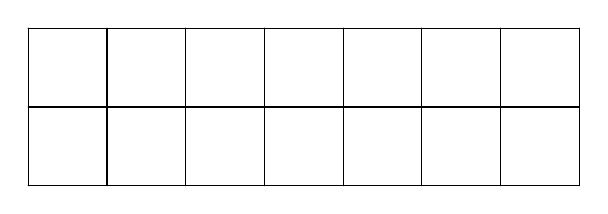
\begin{tikzpicture}[scale=1, font=\footnotesize, line join=round, line cap=round, >=stealth]
    \draw[] (0,0) grid (7,2);			
    \end{tikzpicture}
	\end{center}
	Hai ô vuông gọi là kề nhau nếu có chung một cạnh. Người ta tô màu các ô vuông bởi hai màu đen và đỏ sao cho mỗi ô chỉ được tô đúng một màu. Gọi $P$ là xác suất để có đúng $3$ ô được tô màu đỏ và không có hai ô đỏ nào kề nhau. Giá trị $8\,192P$ bằng bao nhiêu?
	\par\shortans{85}
	\loigiai{
		Số phần tử của không gian mẫu là $n\left(\Omega\right)=2^{14}$.\\
		Gọi $A$ là biến cố \lq\lq có đúng $3$ ô được tô màu đỏ và không có hai ô đỏ nào kề nhau\rq\rq.\\
		Xét các trường hợp sau:
		\begin{enumerate}[\it TH 1:]
			\item $3$ ô đỏ trên 1 hàng và không đứng cạnh nhau.
			\begin{itemize}
				\item Bước 1: Chọn hàng có $2$ cách;
				\item Bước 2: Tô màu $4$ ô đen thành hàng có $1$ cách;
				\item Bước 3: Tô màu $3$ ô đỏ vào $3$ trong $5$ vách ngăn được phân chia bởi $4$ ô đen có $\mathrm{C}_5^3$ cách;
				\item Bước 4: Tô màu các ô còn lại bằng màu đen có $1$ cách.
			\end{itemize}
			Theo quy tắc nhân, trường hợp này có $2\cdot 1\cdot \mathrm{C}_5^3\cdot 1=20$ cách.
			\item $3$ ô đỏ có $2$ ô cùng $1$ hàng, $1$ ô ở hàng còn lại.
			\begin{itemize}
				\item Bước 1: Chọn hàng chứa $2$ ô đỏ có $2$ cách;
				\item Bước 2: Tô màu $2$ ô đỏ ở hàng đó không đứng cạnh nhau có $\mathrm{C}_6^2$ cách;
				\item Bước 3: Tô màu ô đỏ còn lại ở hàng còn lại có $5$ cách;
				\item Bước 4: Tô màu các ô còn lại bằng màu đen có $1$ cách.
			\end{itemize}
			Theo quy tắc nhân, trường hợp này có $2\cdot \mathrm{C}_6^2\cdot 5=150$ cách.
		\end{enumerate}
		Số kết quả thuận lợi cho biến cố $A$ là $n(A)=20+150=170$.\\
		Xác suất $P=\mathrm{P}(A)=\dfrac{170}{2^{14}}=\dfrac{85}{8\,192}$.\\
		Suy ra $8\,192P=85$.
	}
\end{ex}

\begin{ex}%[0D0C2-5]
	\immini[thm]{
		Cho hình vẽ bên gồm $4$ tam giác nhỏ. Người ta chọn $3$ số phân biệt từ tập hợp $S=\{1; 2; \ldots; 26\}$ để xếp vào $3$ tam giác ở $3$ góc. Sau đó, tính tổng bình phương của $3$ số đó rồi ghi kết quả vào tam giác còn lại ở giữa. Hỏi có bao nhiêu cách xếp sao cho số ghi ở tam giác giữa là một số chia hết cho $5$?
	}{
		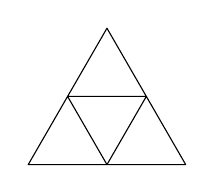
\begin{tikzpicture}[scale=1, line join=round, line cap=round, font=\footnotesize, >=stealth]
    \draw (0,0)--++(0:2)--++(120:2)--cycle
			(1,0)--++(60:1)--++(180:1)--cycle;
    \end{tikzpicture}
	}
	\noindent 	\par\shortans[oly]{3360}
	\loigiai{
		Gọi $3$ số được chọn xếp vào $3$ góc là $a$, $b$, $c \in S$ ($a$, $b$, $c$ phân biệt). \\
		Theo đề bài, ta có số ghi ở tam giác giữa là $a^2+b^2+c^2$. \\
		Để số ghi ở tam giác giữa chia hết cho $5$ thì tổng $a^2+b^2+c^2$ phải chia hết cho $5$. \\
		Xét số dư của bình phương một số nguyên $x$ khi chia cho $5$, ta có
		\begin{itemize}
			\item Nếu $x$ chia hết cho $5$ thì $x^2$ chia hết cho $5$;
			\item Nếu $x$ chia $5$ dư $1$ hoặc $4$ thì $x^2$ chia $5$ dư $1$;
			\item Nếu $x$ chia $5$ dư $2$ hoặc $3$ thì $x^2$ chia $5$ dư $4$.
		\end{itemize}
		Chia tập hợp $S=\{1; 2; \ldots; 26\}$ thành $3$ tập hợp con.
		\begin{itemize}
			\item Tập $A$ gồm các số chia hết cho $5$ là
			\[A=\{5; 10; 15; 20; 25\} \Rightarrow n(A)=5.\]
			\item Tập $B$ gồm các số chia $5$ dư $1$ hoặc $4$ là
			\[B=\{1; 4; 6; 9; 11; 14; 16; 19; 21; 24; 26\} \Rightarrow n(B)=11.\]
			\item Tập $C$ gồm các số chia $5$ dư $2$ hoặc $3$ là
			\[C=\{2; 3; 7; 8; 12; 13; 17; 18; 22; 23\} \Rightarrow n(C)=10.\]
		\end{itemize}
		Do $a^2$, $b^2$, $c^2$ khi chia cho $5$ chỉ có thể nhận các số dư là $0$; $ 1$; $ 4$ nên để tổng $a^2+b^2+c^2$ chia hết cho $5$, ta có các trường hợp sau:
		\begin{enumerate}[\it TH1:]
			\item  Cả ba số $a^2$, $b^2$, $c^2$ đều chia hết cho $5$, tức là $a$, $b$, $c \in A$. \\
			Số cách chọn và xếp $3$ số từ tập $A$ vào $3$ tam giác ở góc (có phân biệt thứ tự) là $\mathrm{A}_5^3=60$ (cách).
			\item Ba số $a^2$, $b^2$, $c^2$ chia cho $5$ có các số dư lần lượt là $0$; $1$; $4$ (vì $0+1+4=5$ chia hết cho $5$). Tức là trong $3$ số $a$, $b$, $c$ có một số thuộc tập $A$, một số thuộc tập $B$, một số thuộc tập $C$. \\
			Số cách chọn và xếp là $3! \cdot \mathrm{C}_5^1 \cdot \mathrm{C}_{11}^1 \cdot \mathrm{C}_{10}^1=6 \cdot 5 \cdot 11 \cdot 10=3\,300$ (cách).
		\end{enumerate}
		Vậy tổng số cách xếp thỏa mãn yêu cầu là $60+3\,300=3\,360$ (cách).
	}
\end{ex}

\begin{ex}%[0D0H2-5]
	Biểu đồ dưới đây thể hiện chi phí hoạt động của $4$ công ty A, B, C, D cho ba hạng mục: Nhân sự, đầu tư và vận hành trong năm $2024$ (đơn vị: tỉ đồng).
	\begin{center}
		\resizebox{!}{6cm}{
			\newcommand{\chuthichbieudo}[2][]{
				\begin{tikzpicture}
					\fill[#1] (0,0) rectangle (\canhhv,\canhhv);
					\path (\canhhv,0)--(\canhhv,\canhhv) node[midway,right]{#2};
				\end{tikzpicture}
			}
			\begin{tikzpicture}[line join = round, line cap = round,>=stealth,font=\footnotesize]
				\def \canhhv{0.4}
				\def \rong{0.7}
				\def \kc{2.5}
				\def \note{{"Công ty A","Công ty B","Công ty C","Công ty D"}}
				\def \cao{{"140","150","125","155"}}
				\def \caohai{{"160","170","165","175"}}
				\def \caoba{{"155","145","160","150"}}
				\def \tongsolieu{4}
				\def\giatrilonnhat{200}
				\pgfmathsetmacro{\tam}{int(\tongsolieu-1)}
				\def \dothuphong{0.019}

				\foreach \i in {0,50,...,\giatrilonnhat}{
					\pgfmathsetmacro{\j}{int(\i*1)}
					\draw[gray!60]
					({\kc-0.5},{\i*\dothuphong}) node[left]{\color{black}$\j$}
					--({(\tam+1)*\kc+(\tam)*\rong+3*\rong+0.5},{\i*\dothuphong});
				}

				\foreach \i in {0,...,\tam}{
					\pgfmathsetmacro{\vb}{\note[\i]}
					\pgfmathsetmacro{\so}{\cao[\i]}
					\pgfmathsetmacro{\sohai}{\caohai[\i]}
					\pgfmathsetmacro{\soba}{\caoba[\i]}

					\draw[pattern=north east lines]
					({(\i+1)*\kc+(\i)*\rong},0)
					rectangle
					({(\i+1)*\kc+(\i+1)*\rong},{\cao[\i]*\dothuphong});

					\draw[pattern=dots]
					($({(\i+1)*\kc+(\i)*\rong},0)+({\rong},0)$)
					rectangle
					({(\i+1)*\kc+(\i+1)*\rong+\rong},{\caohai[\i]*\dothuphong});

					\draw[pattern=north west lines]
					($({(\i+1)*\kc+(\i)*\rong},0)+({2*\rong},0)$)
					rectangle
					({(\i+1)*\kc+(\i+1)*\rong+2*\rong},{\caoba[\i]*\dothuphong});

					\path ({(\i+1)*\kc+(\i)*\rong},0)
					--({(\i+1)*\kc+(\i+1)*\rong+2*\rong+0.2},0)
					node[midway,below]{\vb};

					\path ({(\i+1)*\kc+(\i)*\rong},{\cao[\i]*\dothuphong})
					--({(\i+1)*\kc+(\i+1)*\rong},{\cao[\i]*\dothuphong})
					node[midway,above]{\pgfmathprintnumber[fixed,precision=0,use comma]{\so}};

					\path ({(\i+1)*\kc+(\i)*\rong},0) + ({\rong},{\caohai[\i]*\dothuphong})
					-- ({(\i+1)*\kc+(\i+1)*\rong+\rong},{\caohai[\i]*\dothuphong})
					node[midway,above]{\pgfmathprintnumber[fixed,precision=0,use comma]{\sohai}};

					\path ({(\i+1)*\kc+(\i)*\rong},0) + ({2*\rong},{\caoba[\i]*\dothuphong})
					-- ({(\i+1)*\kc+(\i+1)*\rong+2*\rong},{\caoba[\i]*\dothuphong})
					node[midway,above]{\pgfmathprintnumber[fixed,precision=0,use comma]{\soba}};
				}

				\def \caochuthich{1}
				\path (0,-\caochuthich)
				--({(\tam+1)*\kc+(\tam)*\rong+3*\rong},-\caochuthich)
				node[pos=0.20]{\chuthichbieudo[pattern=north east lines]{Nhân sự}}
				node[pos=0.55]{\chuthichbieudo[pattern=dots]{Đầu tư}}
				node[pos=0.90]{\chuthichbieudo[pattern=north west lines]{Vận hành}};

				\path[xshift=0.8cm] (0,0)--++(0,{\giatrilonnhat*\dothuphong}) node[midway,sloped]{\bf Tỉ đồng};
			\end{tikzpicture}}
	\end{center}
	Chọn ngẫu nhiên một công ty trong các công ty đó. Xác suất để công ty được chọn ra có chi phí trung bình của ba hạng mục lớn hơn $154$ tỉ đồng là
	\choice
		{$\dfrac{1}{4}$}
		{\True $\dfrac{1}{2}$}
		{$\dfrac{2}{3}$}
		{$\dfrac{3}{4}$}
	\loigiai{
		Số lượng các công ty thỏa mãn yêu cầu đề bài:\\
		Công ty A: $\dfrac{140+160+155}{3}=\dfrac{455}{3}\approx 151{,}67<154$ tỉ đồng. (\textbf{Không} thoả mãn)\\\\
		Công ty B: $\dfrac{150+170+145}{3}=\dfrac{465}{3}=155>154$ tỉ đồng. (Thỏa mãn)\\\\
		Công ty C: $\dfrac{125+165+160}{3}=\dfrac{450}{3}=150<154$ tỉ đồng. (\textbf{Không} thoả mãn)\\\\
		Công ty D: $\dfrac{155+175+150}{3}=\dfrac{480}{3}=160>154$ tỉ đồng. (Thoả mãn)\\
		Xác suất để chọn được công ty thỏa mãn yêu cầu đề bài là
		\[ \mathrm{P}=\dfrac{2}{4}=\dfrac{1}{2}. \]
	}
\end{ex}

\begin{ex}%[0D0C2-6]
	\immini[thm]{Trong một trò chơi, có $22$ chiếc đèn được bố trí cách đều nhau trên một vòng tròn lớn (hình vẽ). Khi người chơi bấm nút, hệ thống máy tính sẽ chọn ngẫu nhiên $3$ chiếc đèn để thắp sáng đồng thời. Nếu tâm của vòng tròn nằm hoàn toàn bên trong tam giác tạo bởi $3$ bóng đèn được thắp sáng đó thì người chơi được nhận một phần quà. Mỗi người chơi thực hiện $5$ lần bấm nút. Tính xác suất để một người chơi may mắn giành được ít nhất $2$ phần quà (\textit{không làm tròn kết quả ở các phép tính trung gian, chỉ làm tròn kết quả cuối cùng đến hàng phần trăm}).}
			{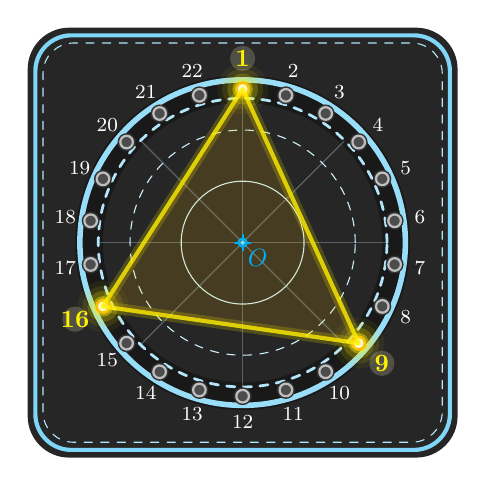
\begin{tikzpicture}[scale=0.65,line cap=round, line join=round, >=stealth, font=\footnotesize]
    \def\R{3} 
				\fill[black!85, rounded corners=15pt] (-4.2, -4.2) rectangle (4.2, 4.2);
				\draw[cyan!50, line width=1.5pt, rounded corners=13pt] (-4.05, -4.05) rectangle (4.05, 4.05);
				\draw[cyan!30, thin, dashed, rounded corners=11pt] (-3.9, -3.9) rectangle (3.9, 3.9);
				\draw[line width=10pt, gray!20!black] (0,0) circle (\R);
				\draw[line width=2pt, cyan!40] (0,0) circle (\R+0.18);
				\draw[line width=1pt, cyan!30, dashed] (0,0) circle (\R-0.18);
				\draw[cyan!20, thin] (0,0) circle (1.2);
				\draw[cyan!20, dashed, thin] (0,0) circle (2.2);
				\foreach \a in {0, 45, ..., 315} {
				\draw[cyan!20, thin, opacity=0.3] (0,0) -- (\a:\R-0.2);
				}
				\foreach \i in {1,...,22} {
				\pgfmathsetmacro{\angle}{90 - (\i-1)*(360/22)}
				\coordinate (L\i) at (\angle:\R);
				}
				\foreach \i in {2,...,8,10,11,12,13,14,15,17,18,19,20,21,22} {
				\pgfmathsetmacro{\angle}{90 - (\i-1)*(360/22)}
				\fill[gray!40!black] (L\i) circle (5pt);
				\fill[black!70, draw=gray!50, thick] (L\i) circle (3.5pt);
				\node[white] at (\angle:\R+0.5) {\i};
				}
				\foreach \i in {1, 9, 16} {
				\pgfmathsetmacro{\angle}{90 - (\i-1)*(360/22)}
				\foreach \r/\op in {0.5/0.05, 0.4/0.1, 0.3/0.2, 0.2/0.4} {
				\fill[yellow, opacity=\op] (L\i) circle (\r);
				}
				\fill[white, draw=yellow!50!orange, line width=1pt] (L\i) circle (3.5pt);
				\fill[yellow!20, opacity=0.2] (\angle:\R+0.6) circle (7pt);
				\node[yellow, font=\bfseries] at (\angle:\R+0.6) {\i};
				}
				\draw[yellow, line width=4pt, opacity=0.2] (L1) -- (L9) -- (L16) -- cycle;
				\draw[yellow, line width=1.5pt, opacity=0.8] (L1) -- (L9) -- (L16) -- cycle;
				\fill[yellow!50!orange, opacity=0.15] (L1) -- (L9) -- (L16) -- cycle;
				\draw[cyan, thick] (-0.15,0) -- (0.15,0);
				\draw[cyan, thick] (0,-0.15) -- (0,0.15);
				\draw[cyan, thick] (0,0) circle (0.08);
				\fill[cyan!50] (0,0) circle (0.04);
				\node[cyan, shift={(-45:0.3)}, inner sep=4pt, font=\bfseries] at (0,0) {$O$};
    \end{tikzpicture}}
			\par
			\shortans{0,29}
	\loigiai{
		Ta có $n(\Omega) = \mathrm{C}_{22}^3 = 1\,540$.\\
		Gọi $A$ là biến cố: \lq\lq Tâm của vòng tròn nằm hoàn toàn bên trong tam giác tạo bởi $3$ bóng đèn\rq\rq.\\
		Vì tâm của vòng tròn nằm hoàn toàn bên trong tam giác khi và chỉ khi tam giác tạo thành là tam giác nhọn nên ta đếm số tam giác nhọn tạo thành từ $22$ đỉnh của đa giác đều nội tiếp đường tròn.\\
		Để tạo ra tam giác vuông từ $3$ trong $22$ đỉnh của đa giác đều, ta cần chọn như sau:
		\begin{itemize}
			\item Chọn $1$ đường chéo trong $11$ đường chéo đi qua tâm của đa giác đều có $11$ cách.
			\item Chọn $1$ đỉnh trong $20$ đỉnh còn lại của đa giác đều có $20$ cách.
		\end{itemize}
		Theo quy tắc nhân, có $11\cdot 20=220$ tam giác vuông có thể tạo thành.\\
		Để tạo ra tam giác tù từ $3$ trong $22$ đỉnh của đa giác đều, ta cần
		\begin{itemize}
			\item Chọn $1$ đỉnh từ $22$ đỉnh của đa giác đều có $22$ cách.
			\item Từ điểm đã chọn, vẽ đường chéo đi qua tâm của đa giác đều, chọn $2$ trong $10$ đỉnh cùng nằm về một phía của đường chéo có $\mathrm{C}_{10}^2$ cách.
		\end{itemize}
		Theo quy tắc nhân, có $22\cdot \mathrm{C}_{10}^2 =990$ tam giác tù được tạo thành.\\
		Vì một tam giác tùy ý chỉ có thể nhọn, vuông hoặc tù nên có $1\,540 - 220 - 990 = 330$ tam giác nhọn có thể tạo thành từ $22$ đỉnh của đa giác.\\
		Suy ra $n(A)=330$.\\
		Xác suất để người chơi nhận được phần quà trong $1$ lần bấm là \[\mathrm{P}(A)=\dfrac{n(A)}{n(\Omega)}=\dfrac{330}{1\,540}=\dfrac{3}{14}.\]
		Khi đó, xác suất để người chơi không nhận được phần quà trong $1$ lần bấm là
		\[\mathrm{P}\left(\overline{A}\right) = 1-\mathrm{P}(A) = 1 - \dfrac{3}{14} = \dfrac{11}{14}. \]
		Gọi $B_i$ là biến cố: \lq\lq Người chơi nhận được đúng $i$ phần quà trong $5$ lần bấm\rq\rq\ $\left( i\in \big\{0;1;2;3;4;5 \big\} \right)$.\\
		Xác suất người chơi không nhận được phần quà nào trong $5$ lần bấm là
		\[\mathrm{P}(B_0) = \mathrm{C}_5^0\cdot \left(\dfrac{3}{14} \right)^0 \cdot \left(\dfrac{11}{14}\right)^5 = \left(\dfrac{11}{14} \right)^5. \]
		Xác suất người chơi nhận được đúng $1$ phần quà trong $5$ lần bấm là
		\[\mathrm{P}(B_1) = \mathrm{C}_5^1\cdot \left(\dfrac{3}{14}\right)^1 \cdot \left(\dfrac{11}{14} \right)^4 = \dfrac{15}{14}\cdot \left(\dfrac{11}{14}\right)^4. \]
		Khi đó, xác suất người chơi nhận được ít nhất $2$ phần quà trong $5$ lần bấm là
		\[1-\big[\mathrm{P}(B_0) + \mathrm{P}(B_1) \big] = 1- \left[\left(\dfrac{11}{14} \right)^5 + \dfrac{15}{14}\cdot \left(\dfrac{11}{14}\right)^4 \right] \approx 0{,}29. \]
	}
\end{ex}

\begin{ex}%[0D0C2-6]
	Cho một bảng ô vuông kích thước $2\times7$ như hình vẽ dưới đây. Hai ô vuông gọi là kề nhau nếu có chung một cạnh. Người ta tô màu các ô vuông bởi hai màu đen và đỏ sao cho mỗi ô chỉ được tô đúng một màu. Gọi $\mathrm{P}$ là xác suất để có đúng 3 ô được tô màu đỏ và không có hai ô đỏ nào kề nhau. Giá trị $8\,192\mathrm{P}$ bằng bao nhiêu?

	\begin{center}
		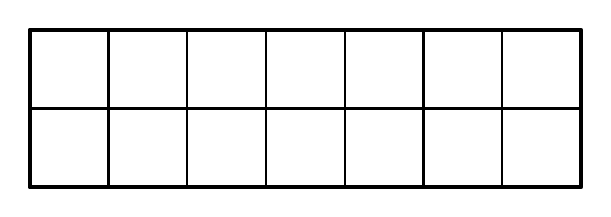
\begin{tikzpicture}[scale=1, font=\footnotesize,line join=round, line cap=round, >=stealth]
			\draw[thick] (0,0) grid (7,2);
			\draw[line width=1.5pt] (0,0) rectangle (7,2);
		\end{tikzpicture}
	\end{center}
	\shortans{$85$}
	\loigiai{
		Mỗi ô vuông có $2$ cách tô màu (đen hoặc đỏ). Tổng số ô vuông là $2 \times 7=14$ ô.\\
		Số phần tử của không gian mẫu là $n(\Omega)=2^{14}=16\,384$.\\
		Gọi biến cố $A\colon $ \lq \lq Có đúng $3$ ô tô màu đỏ và không có hai ô đỏ nào kề nhau\rq \rq.\\
		Do không có hai ô đỏ nào kề nhau nên $3$ ô đỏ không thể nằm chung một cột (nếu chung cột sẽ kề nhau). \\
		Suy ra $3$ ô đỏ phải nằm ở $3$ cột khác nhau trong $7$ cột.\\
		Tổng số cách chọn $3$ cột là $\mathrm{C}_7^3=35$ cách.
		\begin{itemize}
			\item \textbf{Trường hợp 1:} $3$ cột chứa ô đỏ hoàn toàn tách rời nhau (không có $2$ cột nào kề nhau).\\
			Xét $4$ cột còn lại sẽ tạo ra $5$ khoảng trống khi xếp $3$ cột vào $3$ trong $5$ khoảng trống đó sẽ thỏa mãn yêu cầu.\\
			Số cách là $\mathrm{C}_{5}^3=10$ cách.\\
			Với mỗi cách chọn $3$ cột, mỗi cột ta có $2$ cách chọn ô để tô màu đỏ (ô trên hoặc ô dưới).\\
			Số cách tô màu trong trường hợp này là $10 \times 2^3=80$ cách.
			\item \textbf{Trường hợp 2:} Trong $3$ cột chứa ô đỏ, có đúng $2$ cột kề nhau và $1$ cột tách rời.\\
			Ta lấy tổng số trường hợp trừ đi trường hợp $1$ và trường hợp $3$ cột liền nhau thì số cách chọn $2$ cột kề nhau và $1$ cột tách rời là $35-10-5=20$ cách (với $5$ là số cách chọn $3$ cột liên tiếp).\\
			Tại $2$ cột kề nhau: Để $2$ ô đỏ không kề nhau, chúng phải nằm so le ($1$ ô trên, $1$ ô dưới), có $2$ cách tô.\\
			Tại cột tách rời: Ô đỏ có thể nằm ở ô trên hoặc ô dưới, có $2$ cách tô.\\
			Số cách tô màu trong trường hợp này là $20 \cdot  2 \cdot  2=80$ cách.
			\item  \textbf{Trường hợp 3:} $3$ cột chứa ô đỏ kề nhau liên tiếp. Có $5$ cách chọn $3$ cột kề nhau.\\
			Để không có $2$ ô đỏ nào kề nhau, các ô đỏ phải nằm xen kẽ (trên-dưới-trên hoặc dưới-trên-dưới), do đó có $2$ cách tô cho mỗi bộ $3$ cột.\\
			Số cách tô màu trong trường hợp này là $5 \cdot  2=10$ cách.\\

		\end{itemize}
		Tổng số cách tô màu thỏa mãn là $n(A)=80+80+10=170$ cách.\\
		Xác suất của biến cố $A$ là $\mathrm{P}=\dfrac{n(A)}{n(\Omega)}=\dfrac{170}{16\,384}$.\\
		Vậy giá trị cần tìm là: $8\,192P=8\,192\times \dfrac{170}{16\,384}=\dfrac{170}{2}=85$.
	}
\end{ex}

\begin{ex}%[0D0C2-6]
	\immini{Cho một hình bát giác đều có tám đỉnh $A$, $B$, $C$, $D$, $E$, $F$, $G$, $H$. Người ta gắn ngẫu nhiên vào $8$ đỉnh này $8$ số tự nhiên $1$; $2$; $3$; $4$; $5$; $6$; $7$; $8$ (mỗi đỉnh gắn một số). Chọn ngẫu nhiên một tam giác có $3$ đỉnh lấy từ $8$ đỉnh của bát giác đã cho. Gọi $\mathrm{P}$ là xác suất để thu được một tam giác vuông với $3$ số trên $3$ đỉnh của tam giác đó lập thành một cấp số cộng. Biết $P=\dfrac{m}{n}$ (phân số tối giản). Tính $m+3n$}
	{
		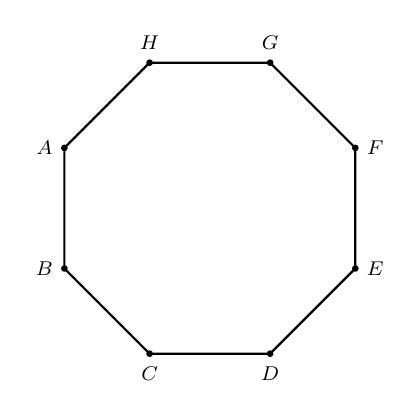
\begin{tikzpicture}[scale=1,>=stealth, line join=round, line cap=round, declare function={R=2;}]
			\path
			(157.5:R) coordinate (A)
			(202.5:R) coordinate (B)
			(247.5:R) coordinate (C)
			(292.5:R) coordinate (D)
			(337.5:R) coordinate (E)
			(22.5:R) coordinate (F)
			(67.5:R) coordinate (G)
			(112.5:R) coordinate (H);
			\draw[thick] (A)--(B)--(C)--(D)--(E)--(F)--(G)--(H)--cycle;
			\foreach \p/\pos in {A/180, B/180, C/-90, D/-90, E/0, F/0, G/90, H/90} {
				\draw[fill=black](\p) circle (1pt) node[shift={(\pos:8pt)}, font=\footnotesize] {$\p$};
			}
		\end{tikzpicture}
	}
	\shortans{303}
	\loigiai{
		Goi $A$ là biến cố \lq\lq Chọn được tam giác vuông\rq\rq.\\
		Tổng số tam giác chọn từ $8$ đỉnh là $\mathrm{C}_8^3$.\\
		Vì bát giác đều nội tiếp đường tròn, tam giác nội tiếp đường tròn đó vuông khi và chỉ khi có một cạnh là đường kính.\\
		Trong bát giác đều có $4$ cặp đỉnh đối diện nên có $4$ đường kính.\\
		Số tam giác vuông là $4\cdot 6=24$.\\
		Do đó, xác suất chọn được một tam giác vuông là $\mathrm{P}(A)=\dfrac{24}{\mathrm{C}_8^3}$.\\ (Vì chọn $1$ đường kính có $4$ cách chọn; chọn đỉnh thứ ba (khác hai đầu đường kính) có $6$ cách chọn).
		\immini{Gọi $B$ là biến cố \lq\lq Tam giác chọn được có các số lập thành cấp số cộng\rq\rq.\\
			Ba số phân biệt lập thành cấp số cộng có dạng: $a$, $a+d$, $a+2d$ với $d \ge 1$.\\
			Trong $\left\lbrace 1;2;..;8\right\rbrace $, ta xét các trường hợp:
			\begin{itemize}
				\item $d=1\colon a=1 \to 6$ nên có $6$ bộ.
				\item $d=2\colon a=1 \to 4$ nên có $4$ bộ.
				\item $d=3\colon a=1 \to 2$ nên có $2$ bộ.
			\end{itemize}
			Tổng cộng có $6+4+2=12$ bộ ba số lập thành cấp số cộng.\\
			Tổng số bộ ba số chọn từ $\left\lbrace 1;2;..;8\right\rbrace $ là $\mathrm{C}_8^3$.
		}
		{
			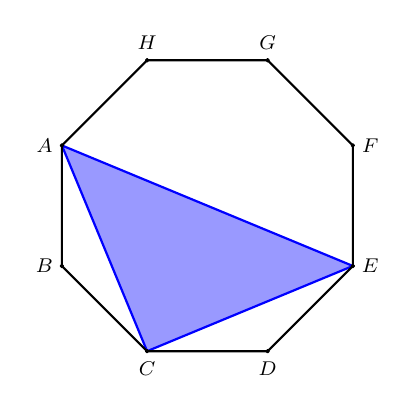
\begin{tikzpicture}[scale=1,>=stealth, line join=round, line cap=round, declare function={R=2;}]
				\path
				(157.5:R) coordinate (A)
				(202.5:R) coordinate (B)
				(247.5:R) coordinate (C)
				(292.5:R) coordinate (D)
				(337.5:R) coordinate (E)
				(22.5:R) coordinate (F)
				(67.5:R) coordinate (G)
				(112.5:R) coordinate (H);
				\fill[blue!40] (A) -- (C) -- (E) -- cycle;
				\draw[blue, thick] (A) -- (C) -- (E) -- cycle;
				\draw[thick] (A)--(B)--(C)--(D)--(E)--(F)--(G)--(H)--cycle;
				\foreach \p/\pos in {A/180, B/180, C/-90, D/-90, E/0, F/0, G/90, H/90} {
					\draw[fill=black] (\p) circle (0.6pt) node[shift={(\pos:7pt)}, font=\footnotesize] {$\p$};
				}
			\end{tikzpicture}
		}
		\noindent Vậy xác suất chọn được bộ ba số lập thành cấp số cộng là $\mathrm{P}(B)=\dfrac{12}{\mathrm{C}_8^3}$.\\
		Việc \lq\lq chọn được tam giác vuông\rq\rq\  phụ thuộc vào hình học chọn đỉnh, còn \lq\lq chọn được cấp số cộng\rq\rq\  phụ thuộc vào các số gắn tại ba đỉnh; do gắn số là ngẫu nhiên nên hai sự kiện độc lập.\\
		Suy ra $\mathrm{P}=\mathrm{P}(A)\cdot\mathrm{P}(B)=\dfrac{24}{\mathrm{C}_8^3} \cdot \dfrac{12}{\mathrm{C}_8^3}=\dfrac{9}{98}=\dfrac{m}{n}$.\\
		Do đó $m=9$, $n=98\Rightarrow m+3n=9+3\cdot98=303$.\\
		Vậy $m+3n=303$.
	}
\end{ex}

\begin{ex}%[0D0V2-6]
	\immini[thm]{Thực hiện chương trình giáo dục phổ thông mới, hàng năm tổ Toán Tin trường THPT Huỳnh Thúc Kháng đều tổ chức chuyên đề ngoại khoá cho học sinh. Trong đó, năm học 2024-2025, tổ đã tổ chức cuộc thi \lq\lq Rung chuông vàng lĩnh vực Toán, Tin\rq\rq cho học sinh cả $3$ khối. Tham gia cuộc thi có $64$ học sinh, trong đó có bạn An và bạn Bình. Sân thi đấu đặt $64$ chiếc ghế đơn xếp thành hình vuông $8\times 8$, mỗi thí sinh tham gia ngồi ngẫu nhiên vào một ghế. Tính xác suất để $2$ bạn An và Bình ngồi cạnh nhau theo hàng dọc hoặc hàng ngang.
	}
	{\resizebox{!}{5cm}{
			
\begin{tikzpicture}[semithick]
				\draw (0,0) rectangle (8,8);
				\foreach \x in{0,2,4,6}{
					\foreach \y in{0,2,4,6}{
						\draw (\x,\y) rectangle (\x+1,\y+1);
					}
				}
				\foreach \x in {1,3,5,7}{
					\foreach \y in {1,3,5,7}{
						\draw (\x,\y) rectangle (\x+1,\y+1);
					}
				}
			\end{tikzpicture}
		}}
	\loigiai{
		\immini{
			Xếp ngẫu nhiên $64$ học sinh vào $64$ chiếc ghế nên không gian mẫu là $n(\Omega)=64!$.\\
			Gọi $A$ là biến cố \lq\lq Hai bạn An và Bình ngồi cạnh nhau theo một hàng ngang hoặc một hàng dọc\rq\rq.\\
			Chọn một hàng ngang hoặc một hàng dọc để xếp An và Bình có $16$ cách.\\
			Trên mỗi hàng hoặc trên mỗi cột, xếp hai bạn an và Bình ngồi gần nhau có $7\cdot 2!=14$ cách.\\
			Sắp xếp $62$ bạn còn lại vào $62$ ghế có $62!$ cách.\\
			Số phần tử của biến cố $A$ là $n(A)=16\cdot 14\cdot 62!$.
		}
		{
			\resizebox{!}{5cm}{
\begin{tikzpicture}
				\draw (0,0) rectangle (8,8);
				\foreach \x/\y in {1/1,1/2,4/5,3/5}
				{
					\fill (\x,\y) rectangle (\x+1,\y+1);
				}
				\foreach \x in{0,2,4,6}{
					\foreach \y in{0,2,4,6}{
						\draw (\x,\y) rectangle (\x+1,\y+1);
					}
				}
				\foreach \x in {1,3,5,7}{
					\foreach \y in {1,3,5,7}{
						\draw (\x,\y) rectangle (\x+1,\y+1);
					}
				}
			\end{tikzpicture}}
	}
	\noindent
	Vậy xác xuất của biến cố $A$ là $\mathrm{P}(A)=\dfrac{n(A)}{n(\Omega)}=\dfrac{16\cdot 14\cdot 62!}{64!}=\dfrac{16\cdot 14}{64\cdot 63}=\dfrac{1}{18}$.
}
\end{ex}

\begin{ex}%[0D0V2-6]
	\immini{
		Một bảng hình vuông kích thước $12 \times 12$ gồm $144$ hình vuông đơn vị, mỗi hình vuông đơn vị có diện tích bằng $1$ (tham khảo hình vẽ).
		Chọn ngẫu nhiên một hình chữ nhật tạo thành từ các hình vuông đơn vị của bảng. Xác suất để hình chữ nhật chọn được có diện tích là một số chẵn bằng $\dfrac{a}{b}$ với $\dfrac{a}{b}$ là phân số tối giản. Khi đó giá trị của $R=a-b$ bằng bao nhiêu?
	}{
		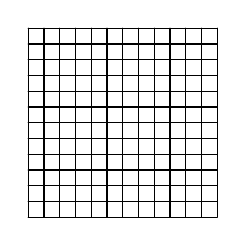
\begin{tikzpicture}[font=\footnotesize, line join=round, line cap=round,>=stealth,scale=.2]
			\draw [black] (0,0) grid (12,12);
		\end{tikzpicture}
	}
	\shortans{$-49$}
	\loigiai{
		Số hình chữ nhật tạo thành từ các hình vuông đơn vị của bảng là $\mathrm C_{13}^2\cdot \mathrm C_{13}^2=78^2=6\,084$.\\
		Diện tích hình chữ nhật là số lẻ khi và chỉ khi chiều dài và chiều rộng đều là số lẻ.\\
		Trên một hàng có $12$ ô, số đoạn có độ dài lẻ là $12+10+8+6+4+2=42$.\\
		Vậy số hình chữ nhật có diện tích lẻ là $42^2=1\,764$.\\
		Số hình chữ nhật có diện tích chẵn là $6\,084-1\,764=4\,320$.\\
		Do đó xác suất cần tìm là $\dfrac{4\,320}{6\,084}=\dfrac{120}{169}$.\\
		Suy ra $a=120,b=169$.\\
		Vậy $R=a-b=120-169=-49$.
	}
\end{ex}

\begin{ex}%[0D0V2-6]
	Trên mặt phẳng tọa độ như hình vẽ, hai điểm $A$ và $B$ cùng lúc bắt đầu di chuyển, mỗi bước đi đúng một đơn~vị theo lưới.
	\begin{center}
		\begin{tikzpicture}[line join=round, line cap=round, >=stealth]
			\draw[->] (-1,0)--(6,0) node[below]{$x$};
			\draw[->] (0,-1)--(0,8) node[right]{$y$};
			\node at (0,0) [below left]{$O$};
			\draw[dashed,thin] (0,0)node[below right]{$A$} grid (5,7)node[above]{$B(5;7)$};
			\fill (0,0) circle (1pt) (5,7) circle (1pt) ;
		\end{tikzpicture}
	\end{center}
	\begin{enumerate}
		\item Điểm $A$ xuất phát từ $O(0;0)$, mỗi bước có thể đi một ô sang phải hoặc một ô lên trên.
		\item Điểm $B$ xuất phát từ $B(5;7)$, mỗi bước có thể đi một ô sang trái hoặc một ô xuống dưới.
	\end{enumerate}
	Giả sử mỗi điểm đều đi đúng $6$ bước và trong số tất cả các đường đi ngắn nhất (đều gồm $6$ bước) thì mỗi đường được chọn với xác suất như nhau.\\
	Hỏi xác suất để hai điểm gặp nhau trên mặt phẳng tọa độ bằng bao nhiêu (làm tròn kết quả đến hàng phần mười).
	\shortans{$0{,}2$}
	\loigiai{
		Hình vẽ
		\begin{center}
			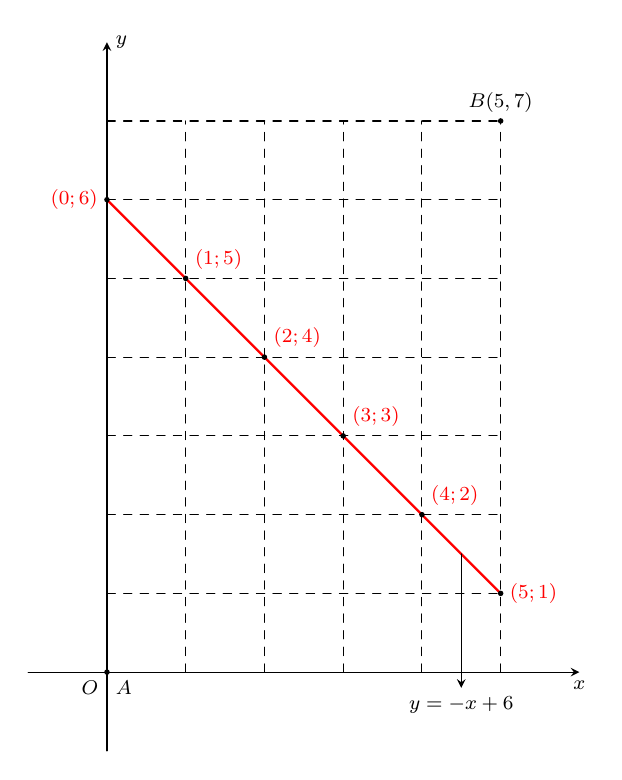
\begin{tikzpicture}[font=\footnotesize, line join=round, line cap=round, >=stealth]
				\draw[->] (-1,0)--(6,0) node[below]{$x$};
				\draw[->] (0,-1)--(0,8) node[right]{$y$};
				\node at (0,0) [below left]{$O$};
				\draw[thick,red] (0,6)node[left]{$(0;6)$}--(1,5)node[above right]{$(1;5)$}--(2,4)node[above right]{$(2;4)$}--(3,3)node[above right]{$(3;3)$}--(4,2)node[above right]{$(4;2)$}--(5,1)node[right]{$(5;1)$};
				\draw[dashed,thin] (0,0)node[below right]{$A$} grid (5,7)node[above]{$B(5,7)$};
				\fill (0,0) circle (1pt) (5,7) circle (1pt) (0,6) circle (1pt) (1,5) circle (1pt) (2,4) circle (1pt) (3,3) circle (1pt) (4,2) circle (1pt) (5,1) circle (1pt) ;
				\draw[->] (4.5,1.5)--(4.5,-0.2)node[below]{$y=-x+6$};
			\end{tikzpicture}
		\end{center}
		Tổng số đường đi hợp lệ của mỗi điểm đều là $\mathrm{C}^0_6+\mathrm{C}^1_6+\mathrm{C}^2_6+\mathrm{C}^3_6+\mathrm{C}^4_6+\mathrm{C}^5_6=63$.\\
		Gọi $M(x;y)$ là điểm gặp nhau sau $6$ bước đi của $A$ và $B$.\\
		Khi đó $x+y=6$ hay $M$ nằm trên đường thẳng $y=-x+6$ và chúng gặp nhau tại các điểm có toạ độ là $(0;6)$, $(1;5)$, $(2;4)$, $(3;3)$, $(4;2)$, $(5;1)$.\\
		Ta có $3$ trường hợp sau
		\begin{itemize}
			\item \textbf{Trường hợp $1$:} Gặp nhau tại $(0;6);(5;1)$ có $1\cdot\dfrac{6!}{5!}\cdot2=12$ cách.
			\item \textbf{Trường hợp $2$:} Gặp nhau tại $(1;5);(4;2)$ có $\dfrac{6!}{5!}\cdot \dfrac{6!}{4!\cdot2!}\cdot 2=6\cdot 15\cdot 2=180$ cách.
			\item \textbf{Trường hợp $3$:} Gặp nhau tại $(2;4);(3;3)$ có $\dfrac{6!}{2!\cdot4!}\cdot \dfrac{6!}{3!\cdot3!}\cdot 2=15\cdot20\cdot2=600$ cách.
		\end{itemize}
		Vậy xác suất để hai điểm gặp nhau trên mặt phẳng tọa độ là $$\dfrac{12+180+600}{63\cdot 63}=\dfrac{88}{441}\approx 0{,}2.$$
	}
\end{ex}

\begin{ex}%[0D0V2-6]
	\immini{
		Cho hàm số $ y=f(x) $ có đạo hàm trên $\mathbb{R}$ và có đồ thị là đường cong $(C)$ như hình bên. Biết rằng đường thẳng $d$ là tiếp tuyến của đồ thị $(C)$ tại điểm $A(2;-1)$. Tiếp tuyến của đồ thị hàm số $y=f^2(1-x)$ tại điểm có hoành độ $x=-1$ có hệ số góc bằng bao nhiêu?
	}
	{
		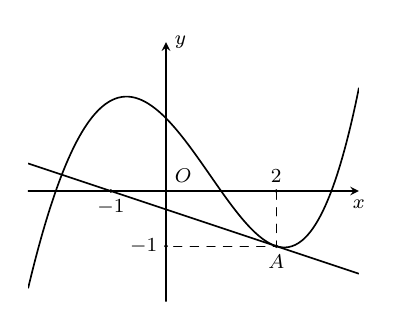
\begin{tikzpicture}[line join=round, line cap=round, >=stealth, font=\footnotesize, scale=.7]
			\pgfmathsetmacro{\xmin}{-2.5}
			\pgfmathsetmacro{\xmax}{3.5}
			\pgfmathsetmacro{\ymin}{-2}
			\pgfmathsetmacro{\ymax}{2.7}

			\draw[->] (\xmin,0)--(\xmax,0) node[below]{$x$};
			\draw[->] (0,\ymin)--(0,\ymax) node[right]{$y$};

			\begin{scope}
				\clip (\xmin,\ymin) rectangle (\xmax,\ymax);
				\draw[thin, semithick] plot[domain=\xmin:\xmax,samples=100,smooth] (\x, { 3/200*(\x)^4+19/100*(\x)^3-103/200*(\x)^2-101/100*\x+33/25});
				\draw[thin, semithick] plot[domain=\xmin:\xmax,samples=100,smooth] (\x, {-1/3*\x-1/3});
			\end{scope}

			\draw[dashed, thin]
			(2,0)--(2,-1)--(0,-1);

			\fill
			(0,0) circle (1pt) node [above right]{$O$}
			(2,-1) circle (1pt) node[below]{$A$}
			(-1,0) circle (1pt) node[below]{$-1$}
			(2,0) circle (1pt) node[above]{$2$}
			(0,-1) circle (1pt) node[left]{$-1$};
		\end{tikzpicture}
	}
	\loigiai{
		Đặt $g(x)=[f(1-x)]^2$. Khi đó
		$$g'(x)=2f(1-x) \cdot f'(1-x) \cdot (-1)=-2f(1-x)\cdot f'(1-x).$$
		Tại $x=-1$, ta có
		$$g'(-1)=-2\cdot f(2)\cdot f'(2).$$\\
		Theo giả thiết, điểm $A(2;-1)$ thuộc đồ thị $(C)$ nên $f(2)=-1$. \\
		Từ đồ thị, tiếp tuyến $d$ tại $A(2;-1)$ có hệ số góc $f'(2)=-\dfrac{1}{3}$. \\
		Do đó
		$$g'(-1)=-2 \cdot (-1) \cdot \left(-\dfrac{1}{3}\right)=-\dfrac{2}{3}.$$
		Vậy hệ số góc cần tìm là $k=-\dfrac{2}{3}$.
	}
\end{ex}

\begin{ex}%[0D0V2-6]
	\immini{Một quân vua được đặt trên một ô giữa bàn cờ vua. Mỗi bước di chuyển, quân vua được chuyển sang một ô khác chung cạnh hoặc chung đỉnh với ô đang đứng (xem hình minh họa). Bạn An di chuyển quân vua ngẫu nhiên $3$ bước. Tính xác suất để sau $3$ bước đi quân
		vua trở về ô xuất phát? Làm tròn kết quả đến hàng phần trăm.
	}{
		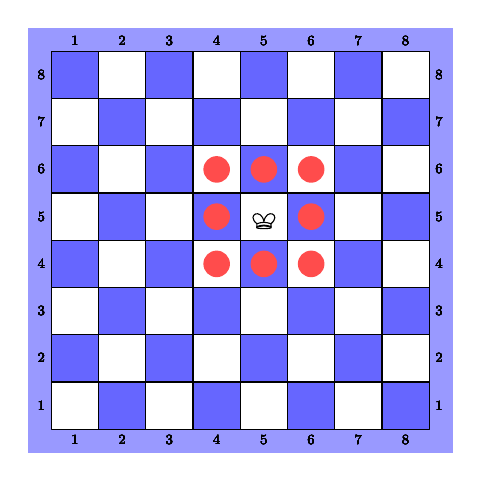
\begin{tikzpicture}[font=\footnotesize,line join=round,line cap=round,>=stealth]
			\begin{scope}[scale=.6]
				\tikzset{vua/.pic={
						\def\a{1}
						\draw ([shift={(0,-\a/4)}]-\a/2,0)--(-\a/2,0)..controls ++ (140:1) and ++(100:1)..(0,0.15)..controls ++(80:1) and ++(40:1)..(\a/2,0)--++(-90:\a/4)..controls++(-30:0.25) and++(-150:0.25)..(-\a/2,-\a/4);
						\foreach \d in {0,\a/5,\a/4}{
							\draw[shift={(0,-\d)}](-\a/2,0)--(-\a/2,0)..controls++(20:0.15) and++(180:0.15)..(0,0.1)..controls++(0:0.15) and++(160:0.15)..(\a/2,0);
						}}}
				\tikzset{vitri/.pic={
						\def\a{0.75}
						\draw[fill=red!70,draw=none,scale=.5](0,0) circle (\a/2);
					}}
				\fill[blue!40](-0.5,-0.5) rectangle (8.5,8.5);
				\foreach \i in{0,1,...,7}
				\foreach \j in{0,1,...,7}
				{
					\pgfmathparse{mod (\i+\j,2)? "blue!60": "white"}
					\fill[\pgfmathresult,draw=black](\i,\j) rectangle (\i+1,\j+1);
					\pgfmathsetmacro{\k}{int (\j+1)}
					\path (0,\j+0.5) node[scale=.7,left]{\k}
					(8,\j+0.5) node[scale=.7,right]{\k}
					(\j+0.5,0) node[scale=.7,below]{\k}
					(\j+0.5,8) node[scale=.7,above]{\k};
				}
				\path (4.5,4.35) pic[scale=0.2]{vua};
				\foreach \x/\y in{5/5,4/5,3/5,3/4,3/3,4/3,5/3,5/4}
				\path[shift={(0.5,0.5)}](\x,\y) pic{vitri};
			\end{scope}
		\end{tikzpicture}
	}
	\shortans{0,05}
	\loigiai{
		Gọi $\Omega$ là không gian mẫu. Từ vị trí của quân vua, cứ mỗi bước sẽ có $8$ vị trí mà quân vua có thể đi. Do đó $|\Omega|=8^3=512$.\\
		Gọi $A$ là biến cố: \lq\lq sau $3$ bước quân vua về ô xuất phát\rq\rq.
		\begin{itemize}
			\item TH1: đi theo hình tam giác vuông cân tại đỉnh vua ban đầu $4\cdot 2=8$ cách.
			\begin{center}
				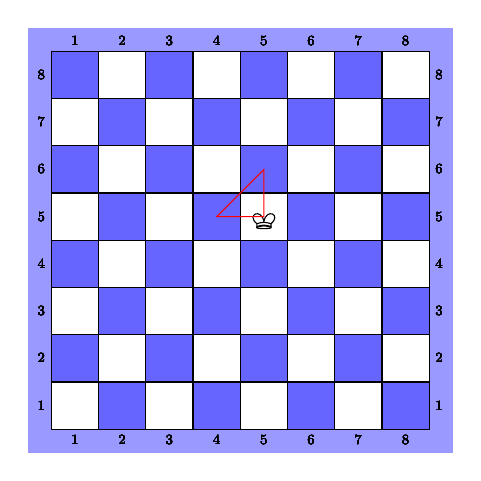
\begin{tikzpicture}[font=\footnotesize,line join=round,line cap=round,>=stealth]
					\begin{scope}[scale=.6]
						\tikzset{vua/.pic={
								\def\a{1}
								\draw ([shift={(0,-\a/4)}]-\a/2,0)--(-\a/2,0)..controls ++ (140:1) and ++(100:1)..(0,0.15)..controls ++(80:1) and ++(40:1)..(\a/2,0)--++(-90:\a/4)..controls++(-30:0.25) and++(-150:0.25)..(-\a/2,-\a/4);
								\foreach \d in {0,\a/5,\a/4}{
									\draw[shift={(0,-\d)}](-\a/2,0)--(-\a/2,0)..controls++(20:0.15) and++(180:0.15)..(0,0.1)..controls++(0:0.15) and++(160:0.15)..(\a/2,0);
								}}}
						\tikzset{vitri/.pic={
								\def\a{0.75}
								\draw[fill=red!70,draw=none,scale=.5](0,0) circle (\a/2);
							}}
						\fill[blue!40](-0.5,-0.5) rectangle (8.5,8.5);
						\foreach \i in{0,1,...,7}
						\foreach \j in{0,1,...,7}
						{
							\pgfmathparse{mod (\i+\j,2)? "blue!60": "white"}
							\fill[\pgfmathresult,draw=black](\i,\j) rectangle (\i+1,\j+1);
							\pgfmathsetmacro{\k}{int (\j+1)}
							\path (0,\j+0.5) node[scale=.7,left]{\k}
							(8,\j+0.5) node[scale=.7,right]{\k}
							(\j+0.5,0) node[scale=.7,below]{\k}
							(\j+0.5,8) node[scale=.7,above]{\k};
						}
						\path (4.5,4.35) pic[scale=0.2]{vua};
						\draw[color=red] (4.5,4.5)--(4.5,5.5)--(3.5,4.5)--(4.5,4.5);
					\end{scope}
				\end{tikzpicture}
			\end{center}
			\item TH2: đi theo hình tam giác vuông cân tại đỉnh khác vua có $8\cdot 2=16$ cách
			\begin{center}
				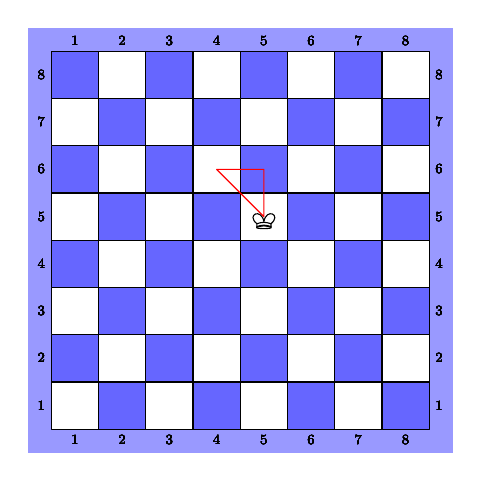
\begin{tikzpicture}[font=\footnotesize,line join=round,line cap=round,>=stealth]
					\begin{scope}[scale=.6]
						\tikzset{vua/.pic={
								\def\a{1}
								\draw ([shift={(0,-\a/4)}]-\a/2,0)--(-\a/2,0)..controls ++ (140:1) and ++(100:1)..(0,0.15)..controls ++(80:1) and ++(40:1)..(\a/2,0)--++(-90:\a/4)..controls++(-30:0.25) and++(-150:0.25)..(-\a/2,-\a/4);
								\foreach \d in {0,\a/5,\a/4}{
									\draw[shift={(0,-\d)}](-\a/2,0)--(-\a/2,0)..controls++(20:0.15) and++(180:0.15)..(0,0.1)..controls++(0:0.15) and++(160:0.15)..(\a/2,0);
								}}}
						\tikzset{vitri/.pic={
								\def\a{0.75}
								\draw[fill=red!70,draw=none,scale=.5](0,0) circle (\a/2);
							}}
						\fill[blue!40](-0.5,-0.5) rectangle (8.5,8.5);
						\foreach \i in{0,1,...,7}
						\foreach \j in{0,1,...,7}
						{
							\pgfmathparse{mod (\i+\j,2)? "blue!60": "white"}
							\fill[\pgfmathresult,draw=black](\i,\j) rectangle (\i+1,\j+1);
							\pgfmathsetmacro{\k}{int (\j+1)}
							\path (0,\j+0.5) node[scale=.7,left]{\k}
							(8,\j+0.5) node[scale=.7,right]{\k}
							(\j+0.5,0) node[scale=.7,below]{\k}
							(\j+0.5,8) node[scale=.7,above]{\k};
						}
						\path (4.5,4.35) pic[scale=0.2]{vua};
						\draw[color=red] (4.5,4.5)--(4.5,5.5)--(3.5,5.5)--(4.5,4.5);
					\end{scope}
				\end{tikzpicture}
			\end{center}
		\end{itemize}
		Do đó $|A|=8+16=24$ cách.\\
		Xác suất để sau $3$ bước đi quân vua về ô xuất phát là $$P(A)=\dfrac{|A|}{|\Omega|}=\dfrac{24}{512}=\dfrac{3}{64}.$$
	}
\end{ex}

\begin{ex}%[0D0C2-9]
	\immini{Một chất điểm chuyển động trên một hình vuông $ABCD$ kích thước $8$ cm $\times$ $8$ cm. Chất điểm di chuyển 
	từ $A$ đến $C$ theo nguyên tắc: mỗi lần di chuyển là một bước nhảy $1$ cm sang phải hoặc lên trên theo các đường 
	kẻ ngang hoặc thẳng đứng trong hình vẽ bên. Tính xác suất để chất điểm đi qua vị trí $M$ được đánh dấu trong hình vẽ bên. 
	\textit{(Làm tròn kết quả đến hàng phần 
		trăm)}. 
	}{\begin{tikzpicture}[scale=0.6, font=\footnotesize]
				\draw[gray!50,thin,opacity=.5]
				(0,0) grid (8,8);
				\path
				(0:0) coordinate (A)
				(4,3) coordinate (M)
				(8,0) coordinate (B)
				(8,8) coordinate (C)
				(0,8) coordinate (D)
				;
				\foreach \x/\g in
				{A/-90,B/-90,C/90,D/90, M/30}
				\fill[black](\x) circle (1.5pt)
				($(\x)+(\g:3mm)$) node{\x};
			\end{tikzpicture}
	} 
		 \shortans{0{,}34} 
	\loigiai{
		 Để di chuyển từ $A$ đến $C$ chất điểm cần thực $8$ bước sang phải và $8$ bước lên trên.\\
		 Do đó có $8+8=16$ bước di chuyển.\\
		Số cách di chuyển từ $A$ đến $C$ là $\mathrm{C}_{16}^8=12\,870$.\\
		Để di chuyển từ $A$ đến $M$ ta thực hiện $4$ bước sang phải và $3$ bước lên trên. \\
		Do đó có $4+3=7$ bước di chuyển.\\
		Số cách di chuyển từ $A$ dến $M$ là $\mathrm{C}_7^3=35$.\\
		Để di chuyển từ $M$ đến $C$ cần thực hiện $4$ bước sang phải và $5$ bước lên trên. \\
		Do đó có $4+5=9$ bước di chuyển.
		Số cách di chuyển từ $M$ dến $C$ là $\mathrm{C}_9^5=126$.\\
		Số cách di chuyển từ $A$ đến $C$ mà đi qua $M$ là
		$35\cdot 126=4\,410$.\\
		Xác suất chất điểm di chuyển từ $A$ đến $C$ mà đi qua $M$ là 
		\[\dfrac{4\,410}{12\,870}=\dfrac{49}{143}\approx 0{,}34.\]
			}
	
\end{ex}

\begin{ex}%[0D0C2-9]
	Trong một trò chơi thám hiểm, anh Sơn phải vượt qua một mê cung gồm các phòng thông nhau như sơ đồ dưới đây. Tại mỗi phòng, anh Sơn sẽ chọn ngẫu nhiên một trong các cửa thông với phòng hiện tại (với xác suất như nhau) để đi tiếp. Quá trình di chuyển diễn ra liên tục và trò chơi sẽ kết thúc ngay khi anh bước vào phòng chứa Kho báu hoặc phòng có Bẫy. Biết anh Sơn bắt đầu từ Phòng 1, xác suất để anh tìm được kho báu bằng bao nhiêu (kết quả làm tròn đến hàng phần trăm)?
	\begin{center}
		\begin{tikzpicture}[scale=1, line join=round, line cap=round, transform shape]
    % --- ĐỊNH NGHĨA MÀU ---
			\definecolor{wood}{HTML}{5D2906}
			\definecolor{gold}{HTML}{FFD700}
			\definecolor{sand}{HTML}{C2B280}
			\def\w{3}
			\def\h{2.5}
			\tikzset{ruong/.pic = {
			\def\g{-130}
			\path (0,0) coordinate (A)
				(\g:2) coordinate (B)
				++(0:4) coordinate (C)
				($(A)+(C)-(B)$) coordinate(D);
			\foreach \i in {A,B,C,D} \path ($(\i)+(90:2.3)$) coordinate(\i');
			\path (D')--++(120:2) coordinate(E) --++(-4,0) coordinate(F);
			\fill[draw, wood!70] (A)--(B)--(B')--(A') (A)--(D)--(D')--(A');
			\draw[wood] (A)--(A');
			\fill[line width=2pt,draw=wood, fill=wood!50] (A')--(B')--(B)--(C)--(D)--(D')--(C')--(B') (A')--(D') (C)--(C');
			\def\NP{(E) .. controls ++(25:0.7) and ++(80:1.5) .. (D') coordinate[pos=0.19](e)}
			\def\NT{(F) .. controls ++(25:0.7) and ++(80:1.5) .. (A')coordinate[pos=0.19](f)};
			\fill[draw, top color=wood!90, middle color=wood!80, bottom color=wood!50] (E)--(F)--\NT -- (D') ..controls ++(80:1.5) and ++(25:0.7) .. (E);
			\fill[draw=wood, fill=gold] (D')--\NP;
			\fill[draw=wood, fill=wood!95] (D')++(105:0.3) coordinate(d') --++(120:1.55) .. controls ++ (25:0.5) and ++(80:1) .. (d');
			\fill[draw=wood, fill=wood!95] (A')--\NT;	
			\fill[draw=wood,wood] ($(A')+(180:1pt)$) -- ++(120:2)--++(0:2pt)--++(-60:2)--cycle ($(D')+(180:2pt)$) -- ++(120:2)--++(0:2pt)--(D')--cycle
				($(E)+(180:2pt)$)--++(180:3.9)--++(-60:2pt)--++(0:3.9)--cycle
				($(D')+(180:2pt)$)--++(180:3.97)--++(-60:2pt)--++(0:3.97)--cycle;
			\fill[draw=gold, gold] (E) .. controls ++(25:0.15)..(e)--(f)..controls ++(170:0.2) and +(70:0.05)..($(F)+(180:1pt)$)--(E);
			\shade[left color=gold!60!brown, right color=gold, middle color=gold!70!white] ($(B)+(-1pt,-1pt)$)--($(C)+(1pt,-1pt)$)--($(C')+(1pt,-1pt)$)--($(B')+(-1pt,-1pt)$)--cycle;
			\shade[left color=gold!40!brown, right color=gold, middle color=gold!70!white] ($(C)+(1pt,-1pt)$)--($(C')+(1pt,-1pt)$)--($(D')+(1pt,-1pt)$)--($(D)+(1pt,-1pt)$)--cycle;
			\fill[wood, rounded corners] ($(B)+(0.24,0.24)$) coordinate(l1) rectangle ++(0.76,1.8) ($(B)+(1.25,0.24)$) coordinate(l2) rectangle ++(1.5,1.8) ($(C)+(-0.24,0.24)$) coordinate(l3) rectangle ++(-0.76,1.8)
				($(C)+(50:0.28)$)++(90:0.24) coordinate(r) --++(50:1.5)--++(90:1.8)--++(\g:1.5)--cycle;
			\begin{scope}
				\clip[rounded corners] (l1) rectangle ++(0.76,1.8);
				\foreach \i in {1,2,3} {\draw[thick, wood!50!black] ($(l1)+(90:0.45*\i)$) --++(0:0.75);}
				\draw[wood!50!black, thick, rounded corners] (l1)--++(90:1.8)--++(0:0.74);
			\end{scope}
			\begin{scope}
				\clip[rounded corners] (l2) rectangle ++(1.5,1.8);
				\foreach \i in {1,2,3} {\draw[thick, wood!50!black] ($(l2)+(90:0.45*\i)$) --++(0:2);}
				\draw[wood!50!black, thick, rounded corners] (l2)--++(90:1.8)--++(0:2);
			\end{scope}
			\begin{scope}
				\clip[rounded corners] (l3) rectangle ++(-0.76,1.8);
				\foreach \i in {1,2,3} {\draw[thick, wood!50!black] ($(l3)+(90:0.45*\i)$) --++(180:1);}
				\draw[wood!50!black, thick, rounded corners] (l3)++(180:0.76)--++(90:1.8)--++(0:1);
			\end{scope}
			\begin{scope}
				\clip[rounded corners] (r) --++(50:1.5)--++(90:1.8)--++(\g:1.5)--cycle;
				\foreach \i in {1,2,3} {\draw[thick, wood!50!black] ($(r)+(90:0.45*\i)$) --++(50:2);}
				\draw[wood!50!black, thick, rounded corners] (r)--++(50:1.5)--++(90:1.8);
			\end{scope}
			\begin{scope}
				\clip (A')--(B')--(C')--(D')--(A');
				\foreach \i in {1,...,500} {
				\shade[ball color=gold] ({random(-10,45)/10}, {random(9,21)/10}) ellipse (0.2 and 0.14);
				}
			\end{scope}
			\fill[draw=gold!80!black, fill=gold, rounded corners] ($(B')!0.43!(C')$)++(-90:0.15) coordinate(k1) rectangle ++(0.6,-0.6);
			\fill (k1)++(0.25,-0.3) arc(-120:300:{0.1}) --++(-90:0.22)--++(180:0.1)--cycle;
			\fill[draw=gold!80!black, fill=gold, rounded corners=0.01] ($(F)!0.43!(E)$) coordinate(k2)--++(\g:0.5)--++(0:0.5)--++(50:0.5)--cycle;
			\fill[black,rotate=-50] (k2)++(0.2,-0.1) ellipse(0.08 and 0.12);}}
			% --- 1. VẼ TƯỜNG MÊ CUNG ---
			% Hàng 1
			\draw (0,\h) -- (0,2*\h) -- (3*\w,2*\h) -- (3*\w,\h);
			% Hàng 2
			\draw (1*\w,0) -- (3*\w,0);
			\draw (3*\w,0) rectangle (4*\w,\h);
			% Các vách ngăn dọc
			\draw (0, \h) -- (1.5*\w, \h); 
			\draw (1.7*\w, \h) -- (3*\w, \h);
			\draw (1*\w, 0) -- (1*\w, 2*\h);
			\draw (2*\w, 0) -- (2*\w, 2*\h); 
			% --- 2. VẼ CỬA THÔNG (Đè đường trắng) ---
			\begin{scope}[white, line width=4pt]
				\draw (\w, 1.3*\h) -- (\w, 1.7*\h); 
				\draw (2*\w, 1.3*\h) -- (2*\w, 1.7*\h); 
				\draw (1.3*\w, \h) -- (1.7*\w, \h); 
				\draw (2.3*\w, \h) -- (2.7*\w, \h); 
				\draw (2*\w, 0.3*\h) -- (2*\w, 0.7*\h); 
				\draw (3*\w, 0.3*\h) -- (3*\w, 0.7*\h); 
			\end{scope}
			% --- 3. CHÈN HÌNH MINH HỌA CHI TIẾT ---	
			% A. CHÈN RƯƠNG KHO BÁU (Tại tọa độ Kho báu)
			\begin{scope}[shift={(0.4*\w, 1.6*\h)}]
				\path (0,0) pic[scale=0.2]{ruong};
			\end{scope}
			% B. CHÈN CẠM BẪY (Tại tọa độ Bẫy)
			\begin{scope}[shift={(3.5*\w, 0.5*\h)}, scale=0.5]
				% Hố chông
				\fill[black!80] (-1,-0.5) rectangle (1,0.5);
				% Chông nhọn
				\foreach \x in {-0.8,-0.4,0,0.4,0.8}
				\fill[gray!60, draw=black, line width=0.2pt] (\x,-0.3) -- (\x-0.15,-0.8) -- (\x+0.15,-0.8) -- cycle;
				\foreach \x in {-0.6,-0.2,0.2,0.6}
				\fill[gray!40, draw=black, line width=0.2pt] (\x,0.1) -- (\x-0.15,-0.4) -- (\x+0.15,-0.4) -- cycle;
				% Biển cảnh báo
				\draw[red, line width=1pt] (0,0.8) -- (-0.6,0) -- (0.6,0) -- cycle;
				\node[red, scale=0.8, font=\boldmath] at (0,0.3) {!};
			\end{scope}
			% --- 4. THÊM VĂN BẢN NHÃN ---
			\node[below] at (0.5*\w, 1.4*\h) {\textbf{Kho báu}};
			\node at (1.5*\w, 1.5*\h) {Phòng 1};
			\node at (2.5*\w, 1.5*\h) {Phòng 2};
			\node at (1.5*\w, 0.5*\h) {Phòng 3};
			\node at (2.5*\w, 0.5*\h) {Phòng 4};
			\node[below] at (3.5*\w, 0.35*\h) {\textbf{Bẫy}};
    \end{tikzpicture}
	\end{center}
	\par
	\shortans{0,67}
	\loigiai{
		Gọi $P_i$ là xác suất để anh Sơn tìm được kho báu nếu đang đứng ở Phòng $i$ ($i=1, 2, 3, 4$). 
		Dựa vào sơ đồ kết nối và quy tắc chọn cửa ngẫu nhiên, ta có hệ phương trình sau:
		\begin{itemize}
			\item Tại Phòng 1 có $3$ cửa (Kho báu, Phòng 2, Phòng 3):
			\[ P_1 = \dfrac{1}{3} \cdot 1 + \dfrac{1}{3} P_2 + \dfrac{1}{3} P_3. \tag*{$(1)$} \]
			\item Tại Phòng 2 có $2$ cửa (Phòng 1, Phòng 4):
			\[ P_2 = \dfrac{1}{2} P_1 + \dfrac{1}{2} P_4. \tag*{$(2)$} \]
			\item Tại Phòng 3 có $2$ cửa (Phòng 1, Phòng 4):
			\[ P_3 = \dfrac{1}{2} P_1 + \dfrac{1}{2} P_4. \quad \tag*{$(3)$} \]
			\item Tại Phòng 4 có $3$ cửa (Phòng 2, Phòng 3, Bẫy):
			\[ P_4 = \dfrac{1}{3} P_2 + \dfrac{1}{3} P_3 + \dfrac{1}{3} \cdot 0. \tag*{$(4)$} \]
		\end{itemize}
		Từ $(2)$ và $(3)$ ta thấy $P_2 = P_3$. Thay vào $(4)$ ta được
		$P_4 = \dfrac{2}{3} P_2$.\\
		Ta được hệ phương trình
		\[ \heva{& P_1 = \dfrac{1}{3} + \dfrac{2}{3} P_2 \\ & P_2 = \dfrac{1}{2} P_1 + \dfrac{1}{2} \left( \dfrac{2}{3} P_2 \right)} 
		\Leftrightarrow \heva{& 3P_1 - 2P_2 = 1 \\ & \dfrac{2}{3} P_2 = \dfrac{1}{2} P_1} 
		\Leftrightarrow \heva{& 3P_1 - 2P_2 = 1 \\ & P_2 = \dfrac{3}{4} P_1}\Rightarrow P_1 = \dfrac{2}{3}. \]
		Làm tròn đến hàng phần trăm, xác suất để anh Sơn tìm được kho báu là $0{,}67$.
	}
\end{ex}

\begin{ex}%[0D0C2-9]
	\immini{
		Một bàn cờ vua gồm $8\times 8$ ô vuông, mỗi ô có cạnh bằng 1 đơn vị. Chọn ngẫu nhiên một hình chữ nhật trên bàn cờ. Xác suất để hình được chọn là một hình vuông có cạnh lớn hơn 4 đơn vị bằng $\dfrac{a}{b}$ với $\dfrac{a}{b}$ là phân số tối giản và $a,b\in \mathbb{N}^*$. Tính giá trị biểu thức $T=a+2b$.
		\shortans{437}
	}{
		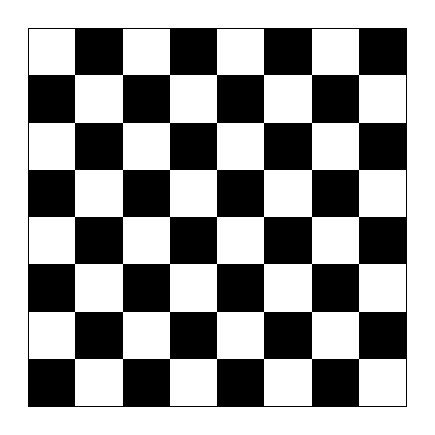
\begin{tikzpicture}[x=1cm,scale=0.6]
			\foreach \x in {0,...,7} \foreach \y in {0,...,7}
			{
				\pgfmathparse{mod(\x+\y,2) ? "white" : "black"}
				\edef\colour{\pgfmathresult}
				\path[fill=\colour] (\x,\y) rectangle ++ (1,1);
			}
			\draw (0,0)--(0,8)--(8,8)--(8,0)--cycle;
		\end{tikzpicture}
	}
	\loigiai{
		Bàn cờ $8\times 8$ cần 9 đoạn thẳng nằm ngang và 9 đoạn thẳng dọc. \\
		Ta coi bàn cờ vua được xác định bởi các đường thẳng $x=0,x=1,\ldots,x=8$ và $y=0,y=1,\ldots,y=8$.\\
		Mỗi hình chữ nhật được tạo thành từ hai đường thẳng nằm ngang $x$ và hai đường thẳng nằm dọc $y$ nên có $\mathrm{C}_9^2\cdot\mathrm{C}_9^2$ hình chữ nhật hay không gian mẫu là $n(\Omega)=\mathrm{C}_9^2\cdot\mathrm{C}_9^2=1296$.\\
		Gọi $A$ là biến cố: \lq\lq  Hình được chọn là hình vuông có cạnh $a$ lớn hơn 4\rq\rq.\\
		\textbf{Trường hợp 1:} $a=5$. Khi đó mỗi ô được tạo thành do 2 đường thẳng $x$ cách nhau 5 đơn vị và hai đường thẳng $y$ cách nhau 5 đơn vị có $4\cdot 4=16$ cách chọn.\\
		\textbf{Trường hợp 2:} $a=6$. Khi đó mỗi ô được tạo thành do 2 đường thẳng $x$ cách nhau 6 đơn vị và hai đường thẳng $y$ cách nhau 6 đơn vị có $3\cdot 3=9$ cách chọn.\\
		\textbf{Trường hợp 3:} $a=7$. Khi đó mỗi ô được tạo thành do 2 đường thẳng $x$ cách nhau 7 đơn vị và hai đường thẳng $y$ cách nhau 7 đơn vị có $2\cdot 2=4$ cách chọn.\\
		\textbf{Trường hợp 4:} $a=8$. Khi đó mỗi ô được tạo thành do 2 đường thẳng $x$ cách nhau 8 đơn vị và hai đường thẳng $y$ cách nhau 8 đơn vị có $1\cdot 1=1$ cách chọn.\\
		Do đó $n(A)=16+9+4+1=30$.\\
		Xác suất để hình được chọn là một hình vuông có cạnh lớn hơn 4 đơn vị là $\mathrm{P}(A)=\dfrac{n(A)}{n(\Omega)}=\dfrac{30}{1296}=\dfrac{5}{321}$. \\
		Suy ra $a=5$, $b=216$. Do đó, $T=a+2b=5+2\cdot 216=437$.
	}
\end{ex}

\begin{ex}%[0D0C2-9]
	\immini[thm]{
		Trong một cuộc thi đấu Robotics, sân đấu được thiết kế dạng lưới ô vuông $4 \times 6$ như hình vẽ. Các robot xuất phát từ vị trí điểm $A$, di chuyển ngẫu nhiên theo cạnh của các ô vuông theo hướng xuống dưới hoặc sang phải đến vị trí điểm $B$. Tính xác suất robot đi từ $A$ đến $B$ mà không đi qua cả $M$ và $N$ (kết quả làm tròn đến hàng phần trăm).
	}{
		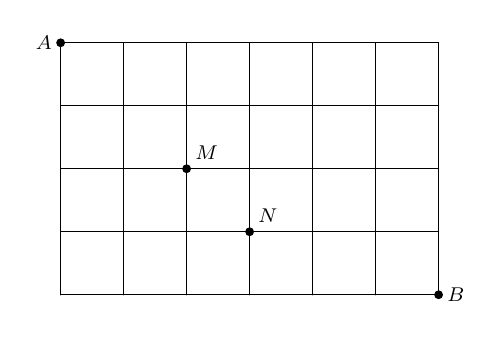
\begin{tikzpicture}[scale=0.8,line join=round, line cap=round, >=stealth, font=\footnotesize]
    % Vẽ lưới 6x4
			\draw (0,0) grid (6,4);			
			\fill (0,4) circle(2pt);
			\fill (6,0) circle(2pt);
			\fill (2,2) circle(2pt);
			\fill (3,1) circle(2pt);
			% Gắn nhãn các điểm
			\node[left] at (0,4) {$A$};
			\node[above right] at (2,2) {$M$};
			\node[above right] at (3,1) {$N$};
			\node[right] at (6,0) {$B$};
    \end{tikzpicture}
	}
	\par
	\shortans[]{0,42}
	\loigiai{
		Để đi từ $A$ đến $B$, robot cần di chuyển $10$ bước gồm $6$ bước sang phải và $4$ bước xuống dưới.\\
		Tổng số đường đi có thể có từ $A$ đến $B$ là $n(\Omega) = \mathrm{C}_{10}^4 = 210$ (đường).\\
		Gọi biến cố $X\colon$\lq\lq Robot đi từ $A$ đến $B$ mà không đi qua cả $M$ và $N$\rq\rq.\\
		Khi đó, biến cố đối $\overline{X}\colon $\lq\lq Robot đi từ $A$ đến $B$ có đi qua $M$ hoặc đi qua $N$\rq\rq.\\
		Ta tính số phần tử của biến cố $\overline{X}$, xét các phương án
		\begin{itemize}
			\item Số đường đi từ $A$ đến $B$ đi qua $M$ (gồm $2$ giai đoạn: $A \to M$ và $M \to B$) là
			\[
			n(M) = \mathrm{C}_4^2 \cdot \mathrm{C}_6^2 = 6 \cdot 15 = 90 \text{ (đường)}.
			\]
			\item Số đường đi từ $A$ đến $B$ đi qua $N$ (gồm $2$ giai đoạn: $A \to N$ và $N \to B$) là
			\[
			n(N) = \mathrm{C}_6^3 \cdot \mathrm{C}_4^1 = 20 \cdot 4 = 80 \text{ (đường)}.
			\]
			\item Số đường đi từ $A$ đến $B$ đi qua cả $M$ và $N$ (gồm $3$ giai đoạn: $A \to M$, $M \to N$ và $N \to B$) là
			\[
			n(M \cap N) = \mathrm{C}_4^2 \cdot \mathrm{C}_2^1 \cdot \mathrm{C}_4^1 = 6 \cdot 2 \cdot 4 = 48 \text{ (đường)}.
			\]
			
		\end{itemize}
		Suy ra số đường đi qua $M$ hoặc $N$ là 
		\[
		n\left(\overline{X}\right) = n(M) + n(N) - n\left(M \cap N\right) = 90 + 80 - 48 = 122 \text{ (đường).} 
		\]
		Vậy xác suất
		\[
		\mathrm{P}(X)=1-\mathrm{P}\left(\overline{X}\right)=1-\dfrac{122}{210}=\dfrac{44}{105}\approx0{,}42.
		\]
	}
\end{ex}

\begin{ex}%[0D0C2-9]
	\immini[thm]{Một con mã đang được đặt ở vị trí chính giữa tâm ô vuông $d4$ trong bàn cờ vua. Thầy Khoa di chuyển con mã $4$ bước để sau $4$ bước đó quân mã quay trở lại vị trí ban đầu với điều kiện $4$ bước đi không trùng nhau. Mỗi bước di chuyển Thầy Khoa đều đặt con mã ở các điểm chính giữa tâm ô vuông đó ($4$ điểm đặt mã sau $4$ bước được xem là $4$ điểm ở tâm ô vuông con mã đi đến). Xác suất để đường đi của con mã có $4$ điểm đặt đó là $4$ đỉnh của một hình vuông có dạng $\dfrac{a}{b}$ (là phân số tối giản, $a$, $b\in\mathbb{N}^*$). Tính $a+2b$.\\
		\textbf{Cách di chuyển của quân Mã} là Mã di chuyển theo đường chéo của hình chữ nhật $2 \times 3$ ô vuông (hoặc $3 \times 2$ ô vuông).}{\begin{tikzpicture}[scale=0.6,  line join=round, line cap=round,  >=stealth, line cap=round, declare function={f(\x)=0;}]
		\draw[thick] (0,0) rectangle (8,8);
		\foreach \x in {0,1,...,7}
		\foreach \y in {0,1,...,7}
		{
			\pgfmathtruncatemacro{\check}{mod(\x+\y,2)}
			\ifnum\check=1
			\fill[gray!70] (\x,\y) rectangle (\x+1,\y+1);
			\fi
		}
		\draw[step=1,black,very thin] (0,0) grid (8,8);
		\foreach \x/\label in {0.5/a, 1.5/b, 2.5/c, 3.5/d, 4.5/e, 5.5/f, 6.5/g, 7.5/h}
		\node at (\x,-0.3) {\footnotesize \label};
		\foreach \y/\label in {0.5/1, 1.5/2, 2.5/3, 3.5/4, 4.5/5, 5.5/6, 6.5/7, 7.5/8}
		\node at (-0.3,\y) {\footnotesize \label};
		\node at (3.5,3.5) {\textbf{M}};
	\end{tikzpicture}}
\par\shortans[0]{26}
\loigiai{
	\underline{\textbf{Cách $1$.}}
	\begin{center}
	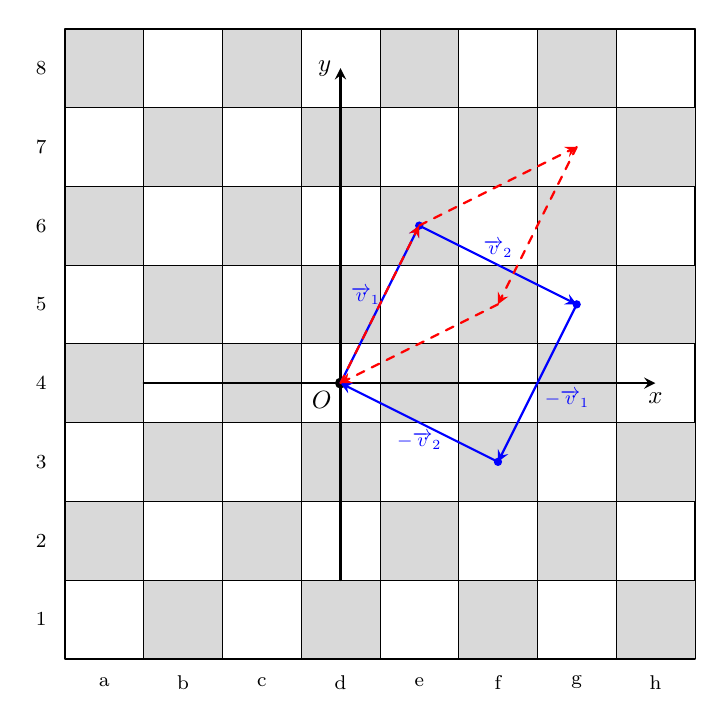
\begin{tikzpicture}[
		scale=1,
		line join=round,
		line cap=round,
		>=stealth
		]
		
		\draw[thick] (0,0) rectangle (8,8);
		
		\foreach \x in {0,1,...,7}
		\foreach \y in {0,1,...,7}
		{
			\pgfmathtruncatemacro{\check}{mod(\x+\y,2)}
			\ifnum\check=1
			\fill[gray!30] (\x,\y) rectangle (\x+1,\y+1);
			\fi
		}
		
		\draw[step=1,black,very thin] (0,0) grid (8,8);
		
		\coordinate (O) at (3.5,3.5);
		
		\draw[->, thick] (1,3.5) --(O)-- ++(4,0)
		node[below] {$x$};
		
		\draw[->, thick] (3.5,1)--(O) -- ++(0,4)
		node[left] {$y$};
		
		\fill (O) circle (2pt) node[below left] {$O$};
		
		\coordinate (A) at (4.5,5.5);
		\coordinate (B) at (6.5,4.5);
		\coordinate (C) at (5.5,2.5);
		
		\draw[blue, thick, ->] (O) -- (A)
		node[midway, above left=-3pt, scale=0.8]
		{$\overrightarrow{v}_1$};
		
		\draw[blue, thick, ->] (A) -- (B)
		node[midway, above, scale=0.8]
		{$\overrightarrow{v}_2$};
		
		\draw[blue, thick, ->] (B) -- (C)
		node[midway, below right, scale=0.8]
		{$-\overrightarrow{v}_1$};
		
		\draw[blue, thick, ->] (C) -- (O)
		node[midway, below=1pt, scale=0.8]
		{$-\overrightarrow{v}_2$};
		
		\fill[blue] (A) circle (1.5pt);
		\fill[blue] (B) circle (1.5pt);
		\fill[blue] (C) circle (1.5pt);
		
		\coordinate (A1) at (4.5,5.5);
		\coordinate (B1) at (6.5,6.5);
		\coordinate (C1) at (5.5,4.5);
		
		\draw[red, dashed, thick, ->] (O) -- (A1);
		\draw[red, dashed, thick, ->] (A1) -- (B1);
		\draw[red, dashed, thick, ->] (B1) -- (C1);
		\draw[red, dashed, thick, ->] (C1) -- (O);
		
		\foreach \x/\label in {
			0.5/a,1.5/b,2.5/c,3.5/d,
			4.5/e,5.5/f,6.5/g,7.5/h
		}
		\node at (\x,-0.3) {\footnotesize \label};
		
		\foreach \y/\label in {
			0.5/1,1.5/2,2.5/3,3.5/4,
			4.5/5,5.5/6,6.5/7,7.5/8
		}
		\node at (-0.3,\y) {\footnotesize \label};
		
	\end{tikzpicture}
\end{center}
	Đặt hệ trục tọa độ có gốc là tâm ô $d4$, ký hiệu là $O(0;0)$.\\
	Mỗi bước đi của quân mã tương ứng với một vectơ $\overrightarrow{v}=(x;y)$ với $x$, $y\in\{\pm 1; \pm 2\}$ và $x^2+y^2=5$ (vì quân mã di chuyển đường chéo của hình chữ nhật kích thước $2\times3$ hoặc $3\times2$).\\
	Suy ra có tất cả $8$ vectơ như vậy, đó là $\overrightarrow{v}_1=(1;2), \overrightarrow{v}_2=(2;1), \overrightarrow{v}_3=(2;-1), \overrightarrow{v}_4=(1;-2), \overrightarrow{v}_5=(-1;-2), \overrightarrow{v}_6=(-2;-1), \overrightarrow{v}_7=(-2;1), \overrightarrow{v}_8=(-1;2).$
	\begin{itemize}
		\item \textbf{Không gian mẫu.} Để quay về $O$ sau $4$ bước không trùng nhau thì các bước đi có dạng vectơ lần lượt là $\overrightarrow{v}_1$; $\overrightarrow{v}_2$; $-\overrightarrow{v}_1$; $-\overrightarrow{v}_2$.
		\begin{itemize}
			\item Chọn $\overrightarrow{v}_1$ có $8$ cách.
			\item Chọn $\overrightarrow{v}_2$ có $6$ cách (loại $\pm \overrightarrow{v}_1$).
		\end{itemize}
		Suy ra $8 \cdot 6=48$ cách.
		\begin{center}
			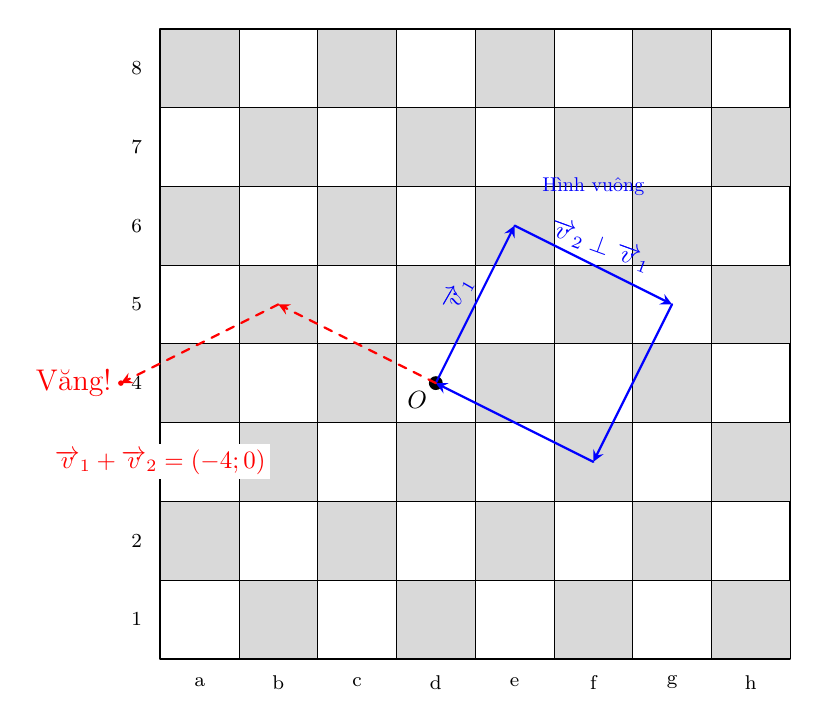
\begin{tikzpicture}[line join=round,line cap=round,>=stealth,scale=1]
				% Vẽ bàn cờ
				\draw[thick] (0,0) rectangle (8,8);
				\foreach \x in {0,1,...,7}{
					\foreach \y in {0,1,...,7}{
						\pgfmathtruncatemacro{\check}{mod (\x+\y,2)}
						\ifnum\check=1
						\fill[gray!30] (\x,\y) rectangle (\x+1,\y+1);
						\fi}}
				\draw[step=1,black,very thin] (0,0) grid (8,8);
				\foreach \x/\l in {0.5/a,1.5/b,2.5/c,3.5/d,4.5/e,5.5/f,6.5/g,7.5/h} \node at (\x,-0.3) {\footnotesize \l};
				\foreach \y/\l in {0.5/1,1.5/2,2.5/3,3.5/4,4.5/5,5.5/6,6.5/7,7.5/8} \node at (-0.3,\y) {\footnotesize \l};
				\coordinate (O) at (3.5,3.5); % Tâm ô d4
				\fill (O) circle (2.5pt) node[below left] {$O$};
				\coordinate (A_v) at (4.5,5.5);
				\coordinate (B_v) at (6.5,4.5);
				\coordinate (C_v) at (5.5,2.5);
				\draw[blue,thick,->] (O) -- (A_v) node[midway,above,rotate=60] {$\overrightarrow{v}_1$};
				\draw[blue,thick,->] (A_v) -- (B_v) node[midway,above,rotate=-20] {$\overrightarrow{v}_2\perp\overrightarrow{v}_1$};
				\draw[blue,thick,->] (B_v) -- (C_v);
				\draw[blue,thick,->] (C_v) -- (O);
				\node[blue,scale=0.8] at (5.5,6) {Hình vuông};
				\coordinate (A_err) at (1.5,4.5); % O + (-2,1)
				\coordinate (B_err) at (-0.5,3.5); % văng khỏi bàn
				\draw[red,dashed,thick,->] (O) -- (A_err);
				\draw[red,dashed,thick,->] (A_err) -- (B_err)
				node[left,scale=1,fill=white] {\large Văng!};
				\fill[red] (B_err) circle (1pt);
				\node[red,scale=1,fill=white,inner sep=2pt] at (0,2.5) {$\overrightarrow{v}_1+\overrightarrow{v}_2=(-4; 0)$};
			\end{tikzpicture}
		\end{center}
		Loại $4$ trường hợp đi chệch khỏi bàn cờ (khi $|x_1+x_2|=4$ hoặc $|y_1+y_2|=4$), ta có $n(\Omega)=48-4=44$.
		\item Gọi $V$ là biến cố \lq\lq đường đi của con mã có $4$ điểm đặt đó là $4$ đỉnh của một hình vuông\rq\rq\ nên $\overrightarrow{v}_1 \perp \overrightarrow{v}_2$. \\
		Với mỗi $\overrightarrow{v}_1$, có $2$ vectơ $\overrightarrow{v}_2$ vuông góc với nó. \\
		Số trường hợp thuận lợi là $8\cdot2=16$ (các hình vuông này đều nằm trong bàn cờ).
	\end{itemize}
	Vì thế $\mathrm{P}(V)=\dfrac{16}{44}=\dfrac{4}{11}$.
	Suy ra $a=4$, $b=11$.\\
	Vậy $a+2b=4+2\cdot11=26$.\\
	\underline{\textbf{Cách 2.}}\\
	Theo giả thiết đề bài (Thầy Khoa di chuyển con mã $4$ bước để sau $4$ bước đó quân mã quay trở lại vị trí ban đầu với điều kiện $4$ bước đi không trùng nhau) thì $4$ bước đi sẽ tạo thành một hình thoi với cạnh là $1$ lần đi.\\
	Khi đấy bước $1$ và bước $3$ và bước $2$ và bước $4$ là những bước phụ thuộc nhau (bước $3$ song song và ngược hướng bước $1$ và ước $4$ song song và ngược hướng bước $2$).\\
	Vì thế ta chỉ quan tâm bước $1$ và $2$.
	\begin{itemize}
		\item Từ vị trí con Mã ($d4$) ta có $8$ cách đi khác nhau cho bước $1$ là các ô vị trí $b3$; $b5$; $c2$; $c6$; $e2$; $e6$; $f3$; $f5$.\\
		Xét các vị trí của bước $1$ ta phân làm $2$ nhóm với tính chất là vị trí cách cạnh bàn cờ với số ô ít nhất là $1$ và $2$. Khi đó
		\begin{itemize}
			\item Nhóm $1$ là cách cạnh bàn cờ ít nhất $2$ ô gồm $c6$; $e6$; $f5$; $f3$. Khi đó bước $1$ có $4$ cách.\\
			Chọn $c6$ làm đại diện của nhóm (vì cùng tính chất) để đi được $4$ bước là cạnh hình thoi thì $c6$ có thể có $6$ cách đi (bước $2$) bao gồm $a5$; $a7$; $b4$; $d8$; $e5$; $e7$.\\
			Vậy ở nhóm $1$ có $4\cdot6=24$ cách.
			\item Nhóm $2$ là cách cạnh bàn cờ ít nhất $1$ ô gồm $b3$; $b5$; $c2$; $e2$. Khi đó bước $1$ có $4$ cách.\\
			Chọn $b3$ làm đại diện của nhóm (vì cùng tính chất) để đi được $4$ bước là cạnh hình thoi thì $b3$ có thể có $5$ cách đi (bước $2$) bao gồm $a1$; $a5$; $c1$; $c5$; $d2$.\\
			Vậy ở nhóm $1$ có $4\cdot5=20$ cách.
		\end{itemize}
		Suy ra $ n(\Omega)=20+24=44$.
		\item Gọi $V$ là biến cố \lq\lq đường đi của con mã có $4$ điểm đặt đó là $4$ đỉnh của một hình vuông\rq\rq.\\
		Chọn bước $1$ đại diện tại ô $c6$ (không mất tính tổng quát), khi đó để đi $4$ bước thành $1$ hình vuông có $2$ cách cho bước $2$ là $a5$ và $e7$.\\
		Suy ra $n(V)=8\cdot2$ cách (bước $1$ có $8$ cách, bước $2$ có $2$ cách và đi theo đường ngược lại vẫn hợp lệ).
	\end{itemize}
	Vì thế $\mathrm{P}(V)=\dfrac{16}{44}=\dfrac{4}{11}$.
	Suy ra $a=4$, $b=11$.\\
	Vậy $a+2b=4+2\cdot11=26$.
}
\end{ex}

\begin{ex}%[0D0H2-9]
	Cho tập $X=\{1;2;3;\ldots;12\}$. Chọn ngẫu nhiên $4$ số phân biệt từ tập $X$ rồi đặt $1$ số vào vòng tròn lớn ở chính giữa, đặt $3$ số còn lại vào ba vòng tròn nhỏ xung quanh (ba vòng tròn nhỏ không phân biệt vị trí). Gọi $\mathrm{P}$ là xác suất để tổng các số tự nhiên trên hai vòng tròn nhỏ bất kì luôn nhỏ hơn số ở vòng tròn lớn chính giữa đồng thời tổng của cả ba số trên ba vòng tròn nhỏ luôn lớn hơn số ở vòng tròn lớn. Tính giá trị của $1\,980\mathrm{P}$.
	\begin{center}
		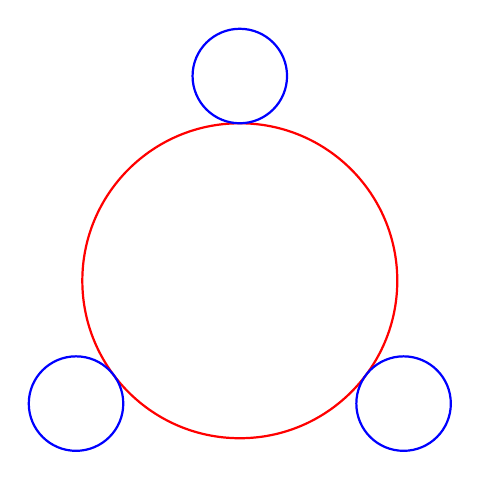
\begin{tikzpicture}[
			scale=1,
			font=\footnotesize,
			line join=round,
			line cap=round,
			>=stealth
			]
			\def\R{2}      % bán kính đường tròn lớn
			\def\r{0.6}    % bán kính đường tròn nhỏ

			% Đường tròn lớn
			\draw[red,thick] (0,0) circle (\R);

			% Đường tròn nhỏ phía trên
			\draw[blue,thick] (0,\R+\r) circle (\r);

			% Đường tròn nhỏ bên trái
			\draw[blue,thick] (-\R*0.8-\r*0.8,-\R*0.6-\r*0.6) circle (\r);

			% Đường tròn nhỏ bên phải
			\draw[blue,thick] (\R*0.8+\r*0.8,-\R*0.6-\r*0.6) circle (\r);
		\end{tikzpicture}
	\end{center}
	\shortans{$16$}
	\loigiai{
		Không gian mẫu của biến cố là $\mathrm{C}_{12}^{4}\cdot \mathrm{C}_{4}^{1}=1\,980$.\\
		Giả sử $4$ số lấy ra bao gồm $a$, $b$, $c$, $M$ trong đó $M$ là số chính giữa và
		$a$, $b$, $c$ $(a<b<c)$ là $3$ số ở ba vòng tròn xung quanh. \\
		Vì $a$, $b$, $c$ không phân biệt thứ tự nên theo yêu cầu bài toán ta có
		$
		\heva{
			&c+b<M<a+b+c\\
			&3<c+b<12.}$\\
		Ta xét các trường hợp có thể xảy ra của số $M$.
		\begin{enumerate}[TH1:]
			\item  $M\in\{1;2;3;4;5;6;7\}$ thì không tồn tại các số $a$, $b$, $c$ thỏa mãn.
			\item $M=8$. Ta có các bộ $(a;b;c)$ thỏa mãn là $(2;3;4)$. Có $1$ bộ.
			\item $M=9$. Ta có các bộ $(a;b;c)$ thỏa mãn là $(2;3;5)$. Có $1$ bộ.
			\item $M=10$. Ta có các bộ $(a;b;c)$ thỏa mãn là
			$(2;3;6)$, $(3;4;5)$, $(2;4;5)$. Có $3$ bộ.
			\item $M=11$. Ta có các bộ $(a;b;c)$ thỏa mãn là $(2;3;7)$, $(2;4;6)$, $(3;4;5)$, $(3;4;6)$. Có $4$ bộ.
			\item $M=12$. Ta có các bộ $(a;b;c)$ thỏa mãn là $(2;3;8)$, $(2;4;7)$, $(3;4;7)$, $(3;4;6)$, $(3;5;6)$, $(4;5;6)$, $(2;5;6)$. Có $7$ bộ.
		\end{enumerate}
		Vậy xác suất của biến cố trên là $\mathrm{P}=\dfrac{16}{1\,980}$.
		Suy ra $1\,980\mathrm{P}=16$.
	}
\end{ex}

\begin{ex} %[0D1N2-1]
	Cho các tập hợp $A$, $B$ được minh họa bằng biểu đồ Ven như hình sau. Phần in đậm trong hình là biểu diễn của tập hợp nào sau đây?
		\begin{center}
		\begin{tikzpicture}
			\def\firstcircle{(0:0) circle (1.2cm)}
			\def\secondcircle{(0:1.8) circle (1.2cm)}
			\begin{scope}
				\clip \firstcircle;
				\fill[pattern=north east lines, gray] \firstcircle;
				\fill[pattern=north east lines, white] \secondcircle;
			\end{scope}
			\draw \firstcircle node[left]{$A$};
			\draw \secondcircle node [right]{$B$};
			%\node[below] () at (0.9,-1.5){$A\cap B$ là phần tô màu vàng};
		\end{tikzpicture}
	\end{center}
	\choice
	{ $A \cap B$}
	{\True $A \setminus B$}
	{ $(A \cup B) \setminus (A \cap B)$}
	{ $B \setminus A$}
	\loigiai{
		Biểu diễn $A \setminus B$.
	}
\end{ex}

\begin{ex}%[0D1N2-1]
	\immini{Cho $A$, $B$ là hai tập hợp được minh họa như hình vẽ. Phần tô bằng các nét gạch trong hình vẽ là tập hợp nào sau đây?
		\choice
		{$B\setminus A$}
		{$A\cup B$}
		{$A\setminus B$}
		{\True $A\cap B$}}
	{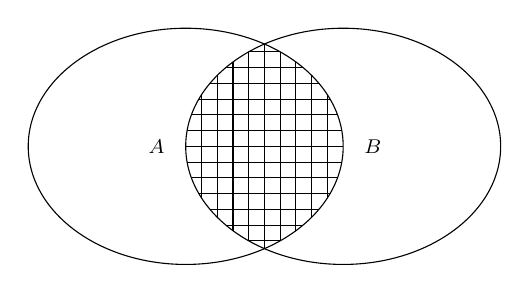
\begin{tikzpicture}[scale=1, font=\footnotesize, line join=round, line cap=round, >=stealth]
			% Vẽ elip A
			\draw (0,0) ellipse (2cm and 1.5cm) node[left=5pt] {$A$}; % Thay circle bằng ellipse
			
			% Vẽ elip B
			\draw (2cm,0) ellipse (2cm and 1.5cm) node[right=5pt] {$B$}; % Thay circle bằng ellipse
			
			% Tô phần giao bằng nét gạch chéo
			\begin{scope}
				\clip (0,0) ellipse (2cm and 1.5cm); % Clip theo elip A
				\clip (2cm,0) ellipse (2cm and 1.5cm); % Clip theo elip B
				
				% Vẽ gạch chéo dọc. Cần điều chỉnh để khớp với hình elip
				\foreach \x in {0.2,0.4,...,1.8} {
					\pgfmathsetmacro\y{1.5*sqrt(1-(\x-1)^2/4)}; % Tính y dựa trên pt elip
					\draw (\x,-\y) -- (\x,\y);
				}
				%Vẽ gạch chéo ngang (tùy chọn để tạo hiệu ứng đậm hơn)
				\foreach \y in {-1.4,-1.2,...,1.4} {
					\pgfmathsetmacro\x{sqrt(4*(1-\y*\y/2.25))+1};
					\draw (2-\x,\y) -- (\x,\y);
				}
			\end{scope}
	\end{tikzpicture}}
	\loigiai{
		Dựa vào hình vẽ ta thấy phần tô bằng nét gạch là tập $A\cap B$.
	}
\end{ex}

\begin{ex}%[0D1N2-1]
	\immini{Viết tập hợp $B$ trong hình dưới bằng cách liệt kê các phần tử của tập hợp đó.
		\choice
		{$B=\left\{a,b,c,d,e\right\}$}
		{$B=\left\{a,b,c\right\}$}
		{$B=\left\{a,b,c,d\right\}$}
		{\True $B=\left\{a,c,d,e\right\}$}}{\begin{tikzpicture}[scale=0.5,line join=round, line cap=round, >=stealth]
			\coordinate (A) at (0,-1);
			\coordinate (B) at (-1,-3);
			\draw[rotate=180] (A) ellipse (4cm and 3cm);
			\begin{scope}[yshift =2]
				%	\draw[rotate=-20](B) ellipse (3cm and 2cm);
			\end{scope}
			\draw(-1,-3.2) node[above ]{$a$};
			\draw(5.5,-2) node[above ]{$b$};
			\draw(.5,-3) node[above ]{$c$};
			\draw(.5,0.6) node[above ]{$d$};
			\draw(-2,-1.4) node[above ]{$e$};
			\draw(1.7,-4)  (-2.7, 2.5)node[right ]{$B$};
			%	\draw(1.5,1)  --(2.5, 1)node[right ]{$C$};
			\fill[black](-1,-3.2)  circle (2pt);
			\fill[black](5.5,-2)  circle (2pt);
			\fill[black](.5,0.5)  circle (2pt);
			\fill[black](.5,-3)   circle (2pt);
			\fill[black](-2,-1.4)  circle (2pt);
	\end{tikzpicture}}
	\loigiai{Tập $B=\left\{a,c,d,e\right\}$.
	}
\end{ex}

\begin{ex}%[0D1H2-2]
	Cho hai tập hợp $A$ và $B$. Hình nào sau đây minh họa $A$ là tập con của $B$?
	\begin{center}
		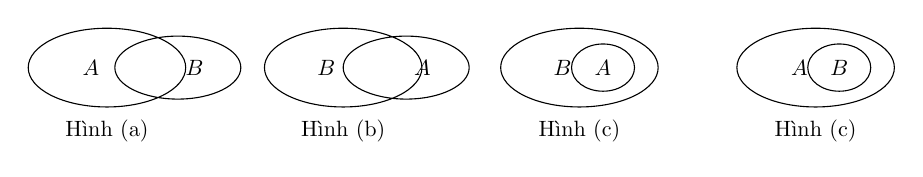
\begin{tikzpicture}[scale = 1,line join=round,line cap=round,>=stealth]
			\tikzset{every node/.style={scale=0.8}}
			\draw (0,0) node[left]{$A$}circle (1 and 0.5) node[yshift=-1.3cm,above]{Hình (a)}
			(0.9,0) node[right]{$B$}circle (0.8 and 0.4);
			\draw [shift={(3,0)}](0,0) node[left]{$B$}circle (1 and 0.5) node[yshift=-1.3cm,above]{Hình (b)}
			(0.8,0) node[right]{$A$}circle (0.8 and 0.4);
			\draw [shift={(6,0)}](0,0) node[left]{$B$}circle (1 and 0.5) node[yshift=-1.3cm,above]{Hình (c)}
			(0.3,0) node{$A$}circle (0.4 and 0.3);
			\draw [shift={(9,0)}](0,0) node[left]{$A$}circle (1 and 0.5) node[yshift=-1.3cm,above]{Hình (c)}
			(0.3,0) node{$B$}circle (0.4 and 0.3);
		\end{tikzpicture}
	\end{center}
	\choice
		{Hình (a)}
		{Hình (b)}
		{\True Hình (c)}
		{Hình (d)}
	\loigiai{Hình (c) là biểu đồ ven, minh họa cho $A\subset B$ vì mọi phần tử của $A$ đều là của $B$.
	}
\end{ex}

\begin{ex}%[0D1N2-2]
Hình vẽ nào sau đây minh họa tập hợp $A$ là tập hợp con của tập hợp $B$?
\begin{center}
\begin{tikzpicture}[line join=round, line cap = round, >=stealth, scale=.8,font=\footnotesize,transform shape]
\draw (1.5,1.5) circle(1.5) (3,1.5) circle(1);
\path (1,1.5) node{$A$}
(3.5,1.5) node{$B$}
(2,-0.3) node{$\text{Hình }1$}
;
\begin{scope}[shift={(5,0)}]
\draw (1.5,1.5) circle(1.5) (3,1.5) circle(1);
\path (1,1.5) node{$B$}
(3.5,1.5) node{$A$}
(2,-0.3) node{$\text{Hình }2$}
;
\end{scope}

\begin{scope}[shift={(10,0)}]
\draw (2,2) circle(2) (2.5,2) circle(1);
\path (1,1.5) node{$B$}
(2.5,1.5) node{$A$}
(2,-0.3) node{$\text{Hình }3$}
;
\end{scope}

\begin{scope}[shift={(15,0)}]
\draw (2,2) circle(2) (2.5,2) circle(1);
\path (1,1.5) node{$A$}
(2.5,1.5) node{$B$}
(2,-0.3) node{$\text{Hình }4$}
;
\end{scope}

\end{tikzpicture}
\end{center}
\choice
{Hình $1$}
{Hình $2$}
{\True Hình $3$}
{Hình $4$}
\loigiai
{
$A\subset B$ khi mọi phần tử của $A$ đều thuộc $B$, tức là miền $A$ nằm hoàn toàn trong miền $B$.\\		
Trong các hình đã cho, chỉ hình $3$ thỏa mãn.
}
\end{ex}

\begin{ex}%[0D1N2-2]
\immini{Cho hai tập hợp $A$ và $B$. Được biểu diễn bằng biểu đồ như hình bên. Khẳng định nào sau đây đúng?
\choice
{$B\subset A$}
{$A=B$}
{$A\cap B=\varnothing $}
{\True $A\subset B$}}{
\begin{tikzpicture}[scale=.6,thick,rotate=-99]
\colorlet{MauNet}{black}
\def\ElipA{(0,0) ellipse (2cm and 3cm)}
\def\ElipB{(0.7,0.7) ellipse (0.7cm and 1.4cm)}
\draw[MauNet,pattern=vertical lines,pattern color=white] \ElipA;
\draw[MauNet,fill=white] \ElipB node[black]{$A$};
\path[MauNet]\ElipA node[above left]{$B$};
\draw[MauNet] (current bounding box.north) node[black,anchor=south] {};
\end{tikzpicture}
}
\loigiai{
}
\end{ex}

\begin{ex}%[0D1N2-2]
	Cho các tập $\mathbb{N}$, $\mathbb{Z}$, $\mathbb{Q}$, $\mathbb{R}$ được minh họa bằng biểu đồ Ven như hình vẽ
	\begin{center}
		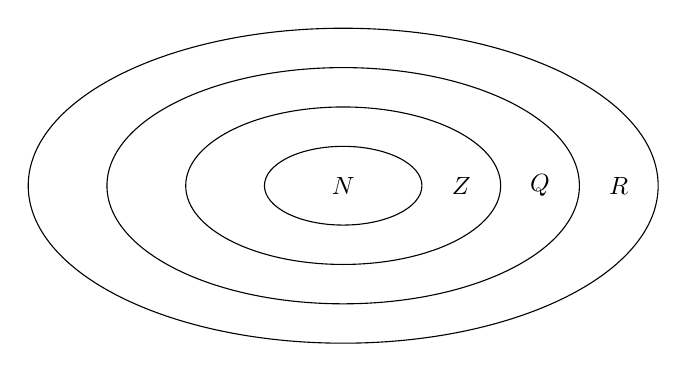
\begin{tikzpicture}
			\draw (0,0) ellipse (4cm and 2cm);
			\node at (3.5,0) {$\mathbb{R}$};
			\draw (0,0) ellipse (3cm and 1.5cm);
			\node at (2.5,0) {$\mathbb{Q}$};
			\draw (0,0) ellipse (2cm and 1cm);
			\node at (1.5,0) {$\mathbb{Z}$};
			\draw (0,0) ellipse (1cm and 0.5cm);
			\node at (0,0) {$\mathbb{N}$};
		\end{tikzpicture}
	\end{center}
	Khẳng định nào dưới đây \textbf{sai}?
	\choice
	{$\mathbb{Z}\subset\mathbb{R}$}
	{$\mathbb{N}\subset\mathbb{R}$}
	{\True $\mathbb{R}\subset\mathbb{Q}$}
	{$\mathbb{N}\subset\mathbb{Q}$}
	\loigiai{
		Khẳng định $\mathbb{R}\subset\mathbb{Q}$ là khẳng định sai.
	}
\end{ex}

\begin{ex}%[0D1H2-3]
Hình vẽ nào sau đây (phần không bị gạch) là hình biểu diễn của $(1;4]$ trên trục số?
\begin{center}

\begin{tikzpicture}[scale=.6, >=stealth, font=\footnotesize]
	\draw[thick, ->] (-2,0)--(7,0);
	\draw 
		(1,0) node {(} node[above] {$1$}
		(4,0) node {)} node[above] {$4$}
		(2.5,-.5) node[below] {Hình 1}
		;
	
	\foreach \x in {-2,-1.8,...,0.8}
		\draw (\x,-0.1)--++(.2,.2);
	\foreach \x in {4.2,4.4,...,6.8}
		\draw (\x,-0.1)--++(.2,.2);
\end{tikzpicture}
\hspace*{3cm}

\begin{tikzpicture}[scale=.6, >=stealth, font=\footnotesize]
	\draw[thick, ->] (-2,0)--(7,0);
	\draw 
		(1,0) node {(} node[above] {$1$}
		(4,0) node {]} node[above] {$4$}
		(2.5,-.5) node[below] {Hình 2}
		;
	
	\foreach \x in {-2,-1.8,...,0.8}
		\draw (\x,-0.1)--++(.2,.2);
	\foreach \x in {4.2,4.4,...,6.8}
		\draw (\x,-0.1)--++(.2,.2);
\end{tikzpicture}
\\

\begin{tikzpicture}[scale=.6, >=stealth, font=\footnotesize]
	\draw[thick, ->] (-2,0)--(7,0);
	\draw 
		(1,0) node {[} node[above] {$1$}
		(4,0) node {]} node[above] {$4$}
		(2.5,-.5) node[below] {Hình 3}
		;
	
	\foreach \x in {-2,-1.8,...,0.8}
		\draw (\x,-0.1)--++(.2,.2);
	\foreach \x in {4.2,4.4,...,6.8}
		\draw (\x,-0.1)--++(.2,.2);
\end{tikzpicture}
\hspace{3cm}

\begin{tikzpicture}[scale=.6, >=stealth, font=\footnotesize]
	\draw[thick, ->] (-2,0)--(7,0);
	\draw 
		(1,0) node {[} node[above] {$1$}
		(4,0) node {)} node[above] {$4$}
		(2.5,-.5) node[below] {Hình 4}
		;
	
	\foreach \x in {-2,-1.8,...,0.8}
		\draw (\x,-0.1)--++(.2,.2);
	\foreach \x in {4.2,4.4,...,6.8}
		\draw (\x,-0.1)--++(.2,.2);
\end{tikzpicture}
\end{center}
\choice
	{Hình 1}
	{\True Hình 2}
	{Hình 3}
	{Hình 4}
\loigiai{
Hình biểu diễn của $(1;4]$ trên trục số là
\begin{center}
	
\begin{tikzpicture}[scale=.6, >=stealth, font=\footnotesize]
	\draw[thick, ->] (-2,0)--(7,0);
	\draw 
		(1,0) node {(} node[above] {$1$}
		(4,0) node {]} node[above] {$4$}
		(2.5,-.5) node[below] {Hình 2}
		;
	
	\foreach \x in {-2,-1.8,...,0.8}
		\draw (\x,-0.1)--++(.2,.2);
	\foreach \x in {4.2,4.4,...,6.8}
		\draw (\x,-0.1)--++(.2,.2);
\end{tikzpicture}
\end{center}
}
\end{ex}

\begin{ex}%[0D1N2-3]
	Phần \textbf{không bị gạch} trong hình vẽ sau đây là biểu diễn của tập hợp nào?
	\begin{center}
		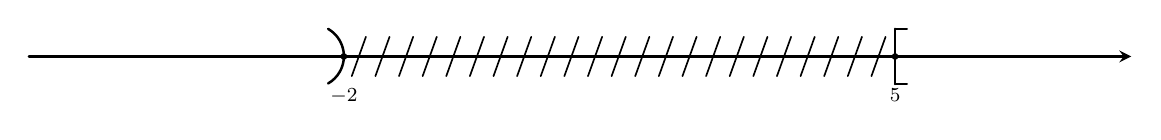
\begin{tikzpicture}[scale=1,font=\footnotesize,line join=round,line cap=round,>=stealth]
			\def\xmin{-6}
			\def\xmax{8}
			\draw[->,line width=0.9pt] (\xmin,0)--(\xmax,0);
			\draw[line width=0.9pt] (-2,0)--(5,0);
			\foreach \x in {-1.9,-1.6,...,4.9}{
				\draw[line width=0.6pt] (\x,-0.25)--(\x+0.18,0.25);
			}
			\draw[line width=0.9pt] (-2.2,0.35) arc(60:-60:0.4);
			\draw[line width=0.9pt] (5,0.35)--(5,-0.35);
			\draw[line width=0.9pt] (5,0.35)--(5.15,0.35);
			\draw[line width=0.9pt] (5,-0.35)--(5.15,-0.35);
			\draw[fill=black] (-2,0) circle (1pt);
			\draw[fill=black] (5,0) circle (1pt);
			\node[below] at (-2,-0.3) {$-2$};
			\node[below] at (5,-0.3) {$5$};
		\end{tikzpicture}
	\end{center}
	\choice
	{$(-\infty;2] \cup (5;+\infty)$}
	{$(-\infty;2] \cup [5;+\infty)$}
	{$(-\infty;2) \cup (5;+\infty)$}
	{\True $(-\infty;2) \cup [5;+\infty)$}
	\loigiai{Dựa vào hình vẽ, ta thấy phần \textbf{không bị gạch} biểu diễn tập hợp $\left(-\infty;2\right)\cup\left[5;+\infty\right)$.}
\end{ex}

\begin{ex}%[0D1N2-3]
	Phần không bị gạch trên trục số dưới đây biểu diễn tập hợp $X$ là một tập con của tập số thực.
	\begin{center}
		\begin{tikzpicture}[line join=round, line cap=round,>=stealth,thick]
			\fill[pattern=north east lines](-6,-0.15)rectangle(-3,0.15);
			\fill[pattern=north east lines](2,-0.15)rectangle(5,0.15);
			\draw[->] (-6,0)--(5,0);
			\draw (-3,0) node {$\big($} (-3,0) node[below=6pt]{$-3$};
			\draw (2,0) node {$\big]$} (2,0) node[below=6pt]{$2$};
		\end{tikzpicture}
	\end{center}
	Mệnh đề nào dưới đây là đúng?
	\choice
	{$X = (-3; 2)$}
	{$X = [-3; 2]$}
	{\True $X = (-3; 2]$}
	{$X = [-3; 2)$}
	\loigiai{
		Ta có $X = (-3; 2]$.
	}
\end{ex}

\begin{ex}%[0D1N2-3]
	Tập hơp $A$ có hình biểu diễn trên trục số như sau
	\begin{center}
		
\begin{tikzpicture}[>=stealth,line join=round,line cap=round,font=\footnotesize,scale=1]
			\draw[->] (2,0)--(8,0);
			\path (6,0) node{$]$} node[below]{$6$};
			\foreach \x in {6.1,6.2,...,7.9} \draw (\x-0.05,-0.1)--(\x+0.05,0.1);
		\end{tikzpicture}
	\end{center}
	$A$ là tập hợp nào sau đây
	\choice
	{$(0;6]$}
	{\True $(-\infty;6]$}
	{$(-\infty;6)$}
	{$(6;+\infty)$}
	\loigiai{
		Tập hơp $A$ có hình biểu diễn trên trục số như trên là tập hợp $(-\infty;6]$.
	}
\end{ex}

\begin{ex}%[0D1N2-3]
	Tập hợp nào dưới đây là tập hợp được biểu diễn trên trục số đã cho?\\
	\begin{center}
		\begin{tikzpicture}[line join=round,line cap=round,>=stealth,font=\footnotesize,scale=1.5]
			\def\a{1}
			\def\b{4}
			\draw[-stealth] (\a-2,0)--(\b+2,0);
			\fill[pattern=north east lines]	(\a-2,-0.1) rectangle (\a,0.1)
			(\b,-0.1) rectangle (\b+2,0.1);
			\path (\a,0) node{$\big($}
			(\b,0) node{$\big)$}
			(\a,-0.4) node{$-2$}
			(\b,-0.4) node{$5$};
		\end{tikzpicture}
	\end{center}
	\choice
	{\True $A=\{x\in \mathbb{R}|-2<x<5\}$}
	{$B=\{x\in \mathbb{R}|-2<x\leq 5\}$}
	{$C=\{x\in \mathbb{R}|-2\leq x\leq 5\}$}
	{$D=\{x\in \mathbb{R}|x\in \mathbb{R} \setminus (-2;5)\}$}
	\loigiai{Trên trục số biểu diễn là khoảng từ $-2$ đến $5$, vì vậy sẽ không chứa hai số $-2$ và $5$.\\
	Vì vậy đáp án là $A=\{x\in \mathbb{R}|-2<x<5\}$.}
\end{ex}

\begin{ex}%[0D1N2-3]
	Hình vẽ dưới là biểu diễn của tập hợp nào sau đây?
	\begin{center}
		\begin{tikzpicture}
			\def\a{-6}
			\def\b{5}
			\draw[-stealth] (\a-2,0)--(\b+2,0);
			\fill[pattern=north east lines]
			(\a,-.1) rectangle (\b,.1);
			%# (\a-2,-.1) rectangle (\a,.1)
			%# (\b,-.1) rectangle (\b+2,.1);
			\path
			(0,0) node{$|$} node[label=-90:$0$]{}
			(\a,0) node{$)$} node[label=-90:${-6}$]{}
			(\b,0) node{$[$} node[label=-90:${5}$]{};
	\end{tikzpicture}\end{center}
	\choice
	{$[-6;5)$}
	{\True $(-\infty;-6)\cup [5;+\infty)$}
	{$(-\infty;-6)\cup (5;+\infty)$}
	{$(-6;5]$}
	\loigiai{
		Hình vẽ biểu diễn tập hợp trục số trên là tập hợp $(-\infty;-6)\cup [5; +\infty)$.
	}
\end{ex}

\begin{ex}%[0D1N2-3]
	Hình vẽ sau đây là biểu diễn của tập hợp nào?
	\begin{center}
		\begin{tikzpicture}[scale=1,>=stealth, font=\footnotesize,line join=round,line cap=round]
			\def\xmin{-5}\def\xmax{5}
			\draw[->] (\xmin,0)--(\xmax,0);
			\path (-2,0)node[shift={(90:5mm)}]{$-2$}(-2,0)node{$\big)$}
			(3,0)node[shift={(90:5mm)}]{$5$}(3,0)node{$\big[$};
			\fill[pattern=north west lines]
			(-2,-0.1) rectangle (3,0.1);
		\end{tikzpicture}
	\end{center}
	\choice
	{$(-\infty;-2] \cup[5;+\infty)$}
	{$(-\infty;-2) \cup(5;+\infty)$}
	{$(-\infty;-2] \cup(5;+\infty)$}
	{\True $(-\infty;-2) \cup[5;+\infty)$}
	\loigiai{
	Ta có $x<-2$ hoặc $x \geq 5$ hay $x \in (-\infty;-2) \cup[5;+\infty)$
	}
\end{ex}

\begin{ex}%[0D1N2-3]
	Cho tập hợp $A$ được biểu diễn trên trục số như sau (phần không bị gạch). Chọn khẳng định đúng trong các khẳng định sau:
	\begin{center}
		\begin{tikzpicture}[scale=1, font=\footnotesize, line join=round, line cap=round, >=stealth]
			\def\xmin{-1};\def\xmax{4};
			(\xmin,0)--(\xmax,0);
			\node (a0) at (1,{0}){[};
			\node (b0) at (2,0){)};
			\draw (a0.-90)node[below]{$1$} (b0.-90)node[below]{$2$};
			\draw[draw=none, pattern=north west lines] ($(a0)+(90:0.1)$)--(\xmin,0.1)--(\xmin,-0.1)--($(a0)+(-90:0.1)$) ($(b0)+(90:0.1)$)--(\xmax,0.1)--(\xmax,-0.1)--($(b0)+(-90:0.1)$);
		\end{tikzpicture}
	\end{center}
	\choice
		{$A=(1;2)$}
		{\True $A=[1;2)$}
		{$A=(1;2]$}
		{$A=(-\infty;1]\cup(2;+\infty)$}
	\loigiai{
		Dựa vào biểu diễn trên trục số, phần không bị gạch biểu diễn tập hợp $A=[1;2)$.
	}
\end{ex}

\begin{ex}%[0D1N2-3]
	Cho tập hợp $A$ được biểu diễn trên trục số như sau (phần không bị gạch). Chọn khẳng định đúng.
	\begin{center}
		\begin{tikzpicture}[scale=1, font=\footnotesize, line join=round, line cap=round, >=stealth]
			\def\xmin{-1};\def\xmax{4};
			(\xmin,0)--(\xmax,0);
			\node (a0) at (1,{0}){[};
			\node (b0) at (2,0){)};
			\draw (a0.-90)node[below]{$1$} (b0.-90)node[below]{$2$};
			\draw[draw=none, pattern=north west lines] ($(a0)+(90:0.1)$)--(\xmin,0.1)--(\xmin,-0.1)--($(a0)+(-90:0.1)$) ($(b0)+(90:0.1)$)--(\xmax,0.1)--(\xmax,-0.1)--($(b0)+(-90:0.1)$);
		\end{tikzpicture}
	\end{center}
	\choice
		{$A=(1;2)$}
		{\True $A=[1;2)$}
		{$A=(1;2]$}
		{$A=(-\infty;1]\cup(2;+\infty)$}
	\loigiai{
		Dựa vào biểu diễn trên trục số, phần không bị gạch biểu diễn tập hợp $A=[1;2)$.
	}
\end{ex}

\begin{ex}%[0D1N2-3]
	Hình vẽ sau đây biểu diễn tập hợp nào?
	\begin{center}
		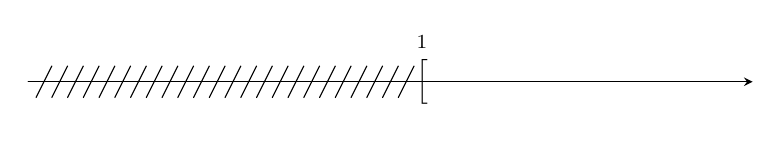
\begin{tikzpicture}[scale=1, font=\footnotesize, line join=round, line cap=round, >=stealth] 
			\draw[->](-4,0) --(5.2,0) node at (1,0.5){$1$}  node at (1,0) {$\Big [$};
			\foreach \b in {-3.8,-3.6,...,0.8} {\draw (\b-0.1,-0.2)--(\b+0.1,0.2);}
		\end{tikzpicture}
	\end{center}
	\choice
	{ $A=\left( 1;+\infty\right) $}
	{ $A=\left( -\infty;1\right] $}
	{$A=\left\lbrace x\in \mathbb{R} \,|\, 1<x\right\rbrace $}
	{\True $A=\left[ 1;+\infty\right) $}
	\loigiai{}
\end{ex}

\begin{ex}%[0D1N2-3]
	Hình vẽ dưới đây biểu diễn tập hợp nào?
	\begin{center}
			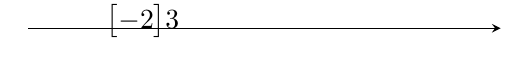
\begin{tikzpicture}[>=stealth]
				\draw[->](-1,0)->(5,0);
				\IntervalLR{-1}{1/2}
				\def\skipInterval{0.5cm}%Khoảng cách đặt nhãn
				\IntervalGRF{}{}{\big[}{$-2$}%Gạch xọc phải qua trái
				\IntervalLR{4}{4.8}
				\def\skipInterval{0.5cm}%Khoảng cách đặt nhãn
				\IntervalGRF{\big]}{$3$}{}{}%Gạch xọc phải qua trái
			\end{tikzpicture}
	\end{center}
	\choice
	{$[-2; 3)$}
	{$(-2; 3]$}
	{\True $[-2; 3]$}
	{$(-2; 3)$}
	\loigiai{
		Hình biểu diễn trục số trên là biểu diễn của đoạn $[-2; 3]$.
	}
\end{ex}

\begin{ex}%[0D1N2-3]%
	Hình vẽ bên dưới biểu diễn tập hợp nào trong các tập sau?
	\begin{center}
		\begin{tikzpicture}[font=\footnotesize, line join=round, line cap=round, >=stealth, scale=1]
			\draw[->] (-1,0) -- (6.2,0);
			\draw (1,0) node {$\big($} node[below=2mm]{$1$}
			(4,0) node {$\big]$} node[below=2mm]{$4$};
			\foreach \x in {-1,-0.8,...,1}{\draw (\x,0) node {$/$};}
			\foreach \x in {4.2,4.4,...,6}{\draw (\x,0) node {$/$};}
		\end{tikzpicture}
	\end{center}
	\choice
	{$(1;4)$}
	{$[1;4)$}
	{$[1;4]$}
	{\True $(1;4]$}
	\loigiai{
		Tập hợp được biểu diễn trên trục số là $(1;4]$.
	}
\end{ex}

\begin{ex}%[0D1H3-1]
	Cho hai tập hợp $A$ và $B$ được mô tả bởi biểu đồ VEN sau đây.
	\begin{center}
		\begin{tikzpicture}[scale=1, font=\footnotesize, line join=round, line cap=round, >=stealth]
			\draw 
			(-1,0) circle (2cm)
			(1,0) circle (2cm)
			;
			\path
			(0,1) node{$1$}
			(0,-1) node{$2$}
			(1.4,1) node{$7$}
			(2,0.6) node{$9$}
			(1.4,-1) node{$11$}
			(-1.4,1) node{$3$}
			(-2,0.6) node{$4$}
			(-1.4,-1) node{$5$}
			(-3.75,0)--++(-45:2) node[below left]{$A$}
			(1.5,0)--++(-45:2) node[below left]{$B$}
			;
		\end{tikzpicture}
	\end{center}
	Khẳng định nào sau đây là \textbf{sai}?
	\choice
	{$A \setminus B=\{3 ; 4 ; 5\}$}
	{$A \cap B=\{1 ; 2\}$}
	{\True$A \cup B=\{3 ; 4 ; 5 ; 7 ; 9 ; 11\}$}
	{$B \setminus A=\{7 ; 9 ; 11\}$}
	\loigiai
	{
		Theo biểu đồ VEN thì $A\cap B=\{1;2\}$.
	}
\end{ex}

\begin{ex}%[0D1H3-1]
	Cho hai tập hợp $A$ và $B$ được mô tả bởi biểu đồ VEN sau đây.
	\begin{center}
		\begin{tikzpicture}[scale=1, font=\footnotesize, line join=round, line cap=round, >=stealth]
			\draw
			(-1,0) circle (2cm)
			(1,0) circle (2cm)
			;
			\path
			(0,1) node{$1$}
			(0,-1) node{$2$}
			(1.4,1) node{$7$}
			(2,0.6) node{$9$}
			(1.4,-1) node{$11$}
			(-1.4,1) node{$3$}
			(-2,0.6) node{$4$}
			(-1.4,-1) node{$5$}
			(-3.75,0)--++(-45:2) node[below left]{$A$}
			(1.5,0)--++(-45:2) node[below left]{$B$}
			;
		\end{tikzpicture}
	\end{center}
	Khẳng định nào sau đây là \textbf{đúng}?
	\choice
		{\True$A \cup B=\{3 ; 4 ; 5 ; 7 ; 9 ; 11\}$}
		{$A \cap B=\{1 ; 2\}$}
		{$B \setminus A=\{7 ; 9 ; 11\}$}
		{$A \setminus B=\{3 ; 4 ; 5\}$}
	\loigiai
	{
		Theo biểu đồ VEN thì $A\cap B=\{1;2\}$.
	}
\end{ex}

\begin{ex}%[0D1N3-1]
	\immini
	{
		Cho $A$, $B$ là hai tập hợp được minh họa như hình vẽ. Phần gạch sọc trong hình vẽ là tập hợp nào sau đây?
		\choice
		{$A\cap B$}
		{$B\setminus A$}
		{$A\cup B$}
		{\True $A\setminus B$}
	}
	{
		\begin{tikzpicture}[scale=0.5, line join=round, line cap=round]
			\coordinate (A) at (0,0);
			\coordinate (B) at (2,0);
			\draw[rotate=45,pattern=north west lines] (A) ellipse (2cm and 1cm) node[above]{$A$}; %cat theo elip A
			\draw[rotate=40,draw=none,fill=white] (B) ellipse (2.2cm and 1.2cm) node[fill=white,above]{$B$};
			\draw[rotate=45] (A) ellipse (2cm and 1cm);
			\draw[rotate=40] (B) ellipse (2.2cm and 1.2cm);
		\end{tikzpicture}	
	}
	
	\loigiai{
		Biểu đồ Ven $A\setminus B$ là tập hợp gồm các phần tử thuộc $A$ nhưng không thuộc $B$.
	}
\end{ex}

\begin{ex}%[0D1N3-1]
	\immini[thm]{Biểu đồ Ven như hình bên phần tô màu thể hiện cho phép toán nào?
		\choice[2]
			{$S\setminus T$}
			{\True $S\cap T$}
			{$S\cup T$}
			{$C_S T$}
	}
	{
		\begin{tikzpicture}[scale=.6, font=\footnotesize, line join=round, line cap=round, >=stealth]
			% 1. Khai báo các tham số bán trục của elip bằng \def
			\def\aI{3.2}
			\def\bI{2.3}
			\def\aII{2.6}
			\def\bII{2.1}
			\def\c{3.8}
			% Khai báo tọa độ tâm của 2 elip
			\path
			(0,0) coordinate (O1)
			(\c,0) coordinate (O2)
			;
			% 2. Tô màu phần giao nhau bằng scope và clip (Dùng màu trắng đen black!15)
			\begin{scope}
				\clip (O1) ellipse ({\aI} and {\bI});
				\fill[black!15] (O2) ellipse ({\aII} and {\bII});
			\end{scope}
			% 3. Vẽ hai đường elip biên biểu đồ Ven (Nét mặc định, màu trắng đen)
			\draw (O1) ellipse ({\aI} and {\bI});
			\draw (O2) ellipse ({\aII} and {\bII});
			% 4. Đặt nhãn S và T vào chính giữa các miền của elip (đã trừ đi phần giao nhau)
			\node at (-1.2,0) {$S$};
			\node at ({\c+1.1},0) {$T$};
		\end{tikzpicture}
	}
	\loigiai{
		Biểu đồ Ven thể hiện cho phép toán lấy giao của hai tập hợp $S$ và $T$.
	}
\end{ex}

\begin{ex}%[0D1N3-1]
	\immini[thm]{Cho $A$, $B$ là hai tập hợp được minh họa như hình vẽ. Phần được gạch trong hình vẽ là tập hợp nào sau đây?
		\choice[2]
			{\True $A\cap B$}
			{$A\cup B$}
			{$A\setminus B$}
			{$B\setminus A$}
	}{
		\begin{tikzpicture}[scale=1.2,font=\footnotesize,line join=round,line cap=round,>=stealth]
			\begin{scope}
				\clip (-0.42,0) ellipse (0.88 and 1.14);
				\fill[pattern=north east lines] (0.45,0) ellipse (0.74 and 0.86);
			\end{scope}
			\draw (-0.42,0) ellipse (0.88 and 1.14);
			\draw (0.45,0) ellipse (0.74 and 0.86);
			\node at (-0.52,0.17) {$A$};
			\node at (0.6,0.15) {$B$};
		\end{tikzpicture}
	}\loigiai{
		Phần được gạch gồm các phần tử vừa thuộc $A$ vừa thuộc $B$. \\
		Do đó, phần này biểu diễn tập hợp $A\cap B$.
	}
\end{ex}

\begin{ex}%[0D1N3-1]
	Cho hai tập hợp $C$ và $G$ có biểu đồ Ven như hình vẽ.
	\immini{
		Hãy xác định tập hợp $C \cap G$.
		\choice
		{\True $C \cap G=\big\{1;2\big\}$}
		{$C \cap G=\big\{3;4;5\big\}$}
		{$C \cap G=\big\{1;2;3;4;5;7;9;11\big\}$}
		{$C \cap G=\big\{7;9;11\big\}$}
	}
	{	\begin{tikzpicture}[scale=0.4]
			\def\firstven{(0,0) ellipse (3cm and 2cm)}
			\def\secondven{(2.5,1) ellipse (2.8cm and 2cm)}
			\draw \firstven \secondven;
			\node at (-2.2,2) {$C$};
			\node at (5.6,2.2){$G$};
			\node at (1,1){$1$};
			\node at (2,-0.1){$2$};
			\node at (-1,0.8){$3$};
			\node at (-2,-0.5){$4$};
			\node at (0,-1){$5$};
			\node at (2.5,2.2){$11$};
			\node at (4,1.5){$7$};
			\node at (3.7,0){$9$};
	\end{tikzpicture}}
	\loigiai{
		Theo biểu đồ Ven ta có $C \cap G=\big\{1;2\big\}$.
	}
\end{ex}

\begin{ex}%[0D1N3-1]
	\immini{
		Cho tập hợp $A$, $B$ được biểu diễn bằng biểu đồ Ven như hình vẽ. Số phần tử của tập $A\cap B$ là
	\choice
	{\True $3$}
	{$8$}
	{$6$}
	{$5$}
}
{
\begin{tikzpicture}		
		\def\ElipA{(0,0) ellipse (3cm and 2cm)}
		\def\ElipB{(1,2) ellipse (2cm and 3cm)}
		\draw\ElipA node[black,below left=1cm] {$A$};
		\draw \ElipB node[black,above right=1cm] {$B$};
		\draw (1,1)node{3} (0.5,0.5)node{4} (1.5,1.5)node{6}
		(-1,0)node{1} (-2,0)node{-2}
		(1,2.5)node{-7} (0.5,3)node{-1} (1.5,3.5)node{5}
		;
	\end{tikzpicture}
}
\loigiai 
{
Ta có $A\cap B=\{3;4;6\}$; nên số phần tử của $A\cap B$ là $3$.
}
\end{ex}

\begin{ex}%[0D1N3-1]
	\immini{Cho $A,B$ là hai tập hợp bất kì. Phần tô đậm trong hình bên là tập hợp nào sau đây?
		\choice
		{\True $A\cap B$}
		{$B \setminus A$}
		{$A\cup B$}
		{$A\setminus B$}
	}{
		\begin{tikzpicture}[scale=0.8, font=\footnotesize, line join=round, line cap=round, >=stealth]
			\def\firstcircle{(0,0) circle (1.5cm)}
			\def\secondcircle{(2,0) circle (1.5cm)}
			\draw \firstcircle node[left] {$A$};
			\draw \secondcircle node [right] {$B$};
			\begin{scope}
				\clip \firstcircle;
				\fill[red] \secondcircle;
			\end{scope}
		\end{tikzpicture}
	}
	\loigiai{
		Hình vẽ trên thể hiện tập  $A\cap B$.
	}
\end{ex}

\begin{ex}%[0D1N3-1]
	\immini{Cho biểu đồ Ven sau đây. Phần được gạch sọc biểu diễn tập hợp nào?
	\choice
	{$B\setminus A$}
	{$A\cap B$}
	{$A\setminus B$}
	{\True $A\cup B$}}
	{\begin{tikzpicture}[thick,rotate=-70,scale=0.4]
			\colorlet{MauNet}{black}
			\def\ElipA{(0,0) ellipse (2cm and 3cm)}
			\def\ElipB{(1,3) ellipse (2cm and 3cm)}
			\draw[MauNet,pattern=north west lines,pattern color=black] \ElipA node[black,below left=1cm] {$A$} \ElipB node[black,above right=1cm]{$B$};
			\draw[MauNet] (current bounding box.north);
	\end{tikzpicture}}
	\loigiai{Phần được gạch sọc biểu diễn tập hợp $A\cup B$.}
\end{ex}

\begin{ex}%[0D1N3-1]
	\immini[thm]{Cho biểu đồ Ven như hình bên, phần tô đậm thể hiện cho phép toán nào?
		\choice[2]
			{$A\cap T$}
			{$A\setminus T$}
			{\True $A\cup T$}
			{$C_A T$}
	}
	{
		\begin{tikzpicture}[scale=.6, font=\footnotesize, line join=round, line cap=round, >=stealth]
			% 1. Khai báo các tham số bán trục của elip bằng \def để tránh lỗi gói book
			\def\xA{0} \def\yA{0} \def\aA{3.5} \def\bA{2.2}
			\def\xT{5.2} \def\yT{0.2} \def\aT{2.5} \def\bT{2.0}
			% Khai báo tọa độ tâm của 2 elip
			\path
			(\xA,\yA) coordinate (OA)
			(\xT,\yT) coordinate (OT)
			;
			% 2. Tô màu nền các miền tập hợp (Sử dụng màu trắng đen chuẩn black!15 cho tài liệu in ấn)
			\fill[black!50] (OA) ellipse ({\aA} and {\bA});
			\fill[black!50] (OT) ellipse ({\aT} and {\bT});
			% 3. Vẽ biên hai elip (Độ dày nét mặc định, màu trắng đen)
			\draw (OA) ellipse ({\aA} and {\bA});
			\draw (OT) ellipse ({\aT} and {\bT});
			% 4. Hiển thị kí hiệu nhãn A và T nằm cân đối bên trong các miền (Môi trường toán $...$)
			\node at (\xA-0.6, \yA-1.0) {$A$};
			\node at (\xT+0.6, \yT-1.0) {$T$};
		\end{tikzpicture}
	}
	\loigiai{
		Biểu đồ Ven thể hiện cho phép toán lấy hợp của hai tập hợp $A$ và $T$.
	}
\end{ex}

\begin{ex}%Câu 2%%[0D1N3-1]
\immini{Cho $A$, $B$ là hai tập hợp được minh họa như hình vẽ. Phần tô đậm trong hình bên dưới là tập hợp nào sau đây?
\choice
{ $A \cup B$}
{\True $A \cap B$}
{$B \setminus A$}
{$A \setminus B$}}
{\begin{tikzpicture}
\def\miena{(0,0)to [bend left=90] (2,2) to[bend left=90] (0,0) }
\def\mienb{(1,0)to [bend left=90] (3,2) to[bend left=90] (1,0) }
\begin{scope}
\clip \miena;
\draw[pattern=north east lines] \mienb;
\end{scope}
\draw \miena \mienb;
\draw (0.2,0.5)node[above]{$A$} (2.6,1.3)node[above]{$B$};
\end{tikzpicture}}
\loigiai{ Phần tô đậm là $A\cap B$.
}
\end{ex}

\begin{ex}%[0D1N3-1]
	\immini{
		Cho tập hợp $A$, $B$ được biểu diễn bằng biểu đồ Ven như hình vẽ. Số phần tử của tập $A\cap B$ là
		\choice
			{$8$}
			{$5$}
			{$6$}
			{\True $3$}
	}
	{
		\begin{tikzpicture}
			\def\ElipA{(0,0) ellipse (3cm and 2cm)}
			\def\ElipB{(1,2) ellipse (2cm and 3cm)}
			\draw\ElipA node[black,below left=1cm] {$A$};
			\draw \ElipB node[black,above right=1cm] {$B$};
			\draw (1,1)node{3} (0.5,0.5)node{4} (1.5,1.5)node{6}
			(-1,0)node{1} (-2,0)node{-2}
			(1,2.5)node{-7} (0.5,3)node{-1} (1.5,3.5)node{5}
			;
		\end{tikzpicture}
	}
	\loigiai
	{
		Ta có $A\cap B=\{3;4;6\}$; nên số phần tử của $A\cap B$ là $3$.
	}
\end{ex}

\begin{ex}%[0D1N3-1]
	Phần tô màu trong hình bên là biểu diễn của tập hợp nào dưới đây?
	\begin{center}
		\begin{tikzpicture}[>=stealth,line join=round,line cap=round,font=\footnotesize,scale=1]
			\def\firstellipse{(0.5,0) ellipse (1.5 and 1)}
			\def\secondellipse{(2.5,0) ellipse (2 and 1)}
			\draw[fill=blue!30] \firstellipse \secondellipse;
			%\path (current bounding box.south) node[below=2mm]{$A\cup B$};
			\node at (-0.5,0){$A$};
			\node at (3.5,0){$B$};
		\end{tikzpicture}
	\end{center}
	\choice
	{$B\setminus A$}
	{$A\setminus B$}
	{$A\cap B$}
	{\True $A\cup B$}
	\loigiai{
		Phần tô màu trong hình vẽ là hình biểu diễn của tập $A\cup B$.
	}
\end{ex}

\begin{ex}%[0D1N3-1]
	\immini{Hình vẽ bên biểu diễn phép toán nào của hai tập hợp $A$ và $B$}
	{
	\begin{tikzpicture}[scale=1, font=\footnotesize, line join=round, line cap=round, >=stealth]
		% Tập hợp thứ nhất (bôi màu)
		\draw [pattern=north east lines] (0,0) to[bend left=90] (2,2);
		\draw [pattern=north east lines] (2,2) to[bend left=90] (0,0);
		% Tập hợp thứ hai (bôi màu)
		\draw [pattern=north east lines] (1,0) to[bend left=90] (3,2);
		\draw [pattern=north east lines] (3,2) to[bend left=90] (1,0);
	%	\draw (1.5,-1) node{$A \cup B$};
	\end{tikzpicture}
	}
	\choice
	{$A\in B$}
	{\True $A\cup B$}
	{$A \le B$}
	{$A\cap B$}
	\loigiai{
	$A \cup B$
	}
\end{ex}

\begin{ex}%[0D1N3-1]	
	\immini{
		Cho $A$, $B$ là hai tập hợp bất kì khác tập rỗng, được biểu diễn theo biểu đồ Ven sau. Phần gạch sọc trong hình vẽ là tập hợp nào sau đây?
		\choice
		{$B \setminus A$}
		{\True $A \cap B$}
		{$A \cup B$}
		{$A \setminus B$}
	}{
		\begin{tikzpicture}[line join = round, line cap=round,>=stealth,font=\footnotesize,scale=0.8]
			\def\firstcircle{(0,0) circle (1.5cm)}
			\def\secondcircle{(2,0) circle (1.5cm)}
			\begin{scope}
				\clip \firstcircle;
				\fill[pattern=north east lines, pattern color=green!50!black] \secondcircle;
			\end{scope}
			\draw[thick, blue] \firstcircle;
			\draw[thick, blue] \secondcircle;
			\node at (-0.5,0) {$A$};
			\node at (2.5,0) {$B$};
		\end{tikzpicture}
	}
	\loigiai{
		Quan sát biểu đồ Ven, ta thấy phần gạch sọc là phần chung của hai tập hợp $A$ và $B$. \\
		Do đó, phần gạch sọc biểu diễn cho tập hợp giao $A \cap B$.
	}
\end{ex}

\begin{ex}%[0D1N3-1]
	Cho biểu đồ Ven sau đây. Phần được gạch sọc biểu diễn tập hợp nào?
	\begin{center}
	\begin{tikzpicture}[>=stealth,line join=round,line cap=round,font=\footnotesize,scale=1]
	\def\firstellipse{(0.5,0) ellipse (1.5 and 1)}
	\def\secondellipse{(2.5,0) ellipse (2 and 1.5)}
	\begin{scope}
	\clip \firstellipse ;
	\fill[pattern=north east lines] \secondellipse;
	\end{scope}
	\draw \firstellipse \secondellipse;
	\node at (-0.5,0){$A$};
	\node at (3.5,0){$B$};
	\end{tikzpicture}
	\end{center}
	\choice
	{$B \setminus A$}
	{$A \setminus B$}
	{$A \cup B$}
	{\True $A \cap B$}
	\loigiai{
	Phần được gạch sọc trong biểu đồ Ven phép giao của hai tập hợp, ký hiệu là $A \cap B$.
	}
\end{ex}

\begin{ex}%[0D1N3-1]
	\immini{Cho các tập hợp $A,B$ được minh hoạ bằng biểu đồ Ven như hình vẽ. Phần gạch sọc trong hình là biểu diễn của tập hợp nào sau đây?
		\choice
		{$A\cap B$}
		{$A\setminus B$}
		{$\mathrm{C}_BA$}
		{\True $A\cup B$}}{\begin{tikzpicture}[thick, scale=.8]
			\def\a{1.3}\def\r{2}
			\path (0:\a) coordinate (A) (180:\a) coordinate (B);
			\fill[pattern=north west lines]
			(B) circle (\r cm) 
			(A) circle (\r cm);
			\foreach \x in {A,B} \draw (\x) circle (\r cm);
			\node[] at (A) {$ B $};
			\node[] at (B) {$ A $};
	\end{tikzpicture}}
	\loigiai{Phần gạch sọc trong hình là biểu diễn của tập hợp $A\cup B$.
	}
\end{ex}

\begin{ex}%Câu 8%[0D1H3-2]
\immini{Cho hai tập hợp $A$ và $B$ được minh hoạ bằng biểu đồ hình Ven như hình vẽ. Phần tô đậm trong hình là biểu diễn của tập hợp nào sau đây?
\choice 
{ $A \cap B$}
{$A \cup B$}
{$B \setminus A$}
{\True $A \setminus B$}}	
{	\begin{tikzpicture}[scale=1, font=\footnotesize, line join=round, line cap=round, >=stealth]
		\def\miena{(0,0) to [bend left=90] (2,2) to [bend left=90] (0,0)}
		\def\mienb{(1,0) to [bend left=90] (3,2) to [bend left=90] (1,0)}
		\fill[pattern=north east lines] \miena;
		\draw[fill=white]\mienb (0.3,1) node{$A$} (2.55,1.5) node{$B$};
		\draw \miena;
\end{tikzpicture}}



\loigiai{%
}
\end{ex}

\begin{ex}%[0D1H3-2]
	Cho $A,B,C$ là các tập hợp được biểu diễn minh họa bên dưới. Cho tập $D$ là phần giao được tô đậm. Khi đó tập $D$ sẽ tương đương phép tính tập hợp nào dưới đây?
	\begin{center}
		\begin{tikzpicture}[line join=round,line cap=round,>=stealth,font=\footnotesize,scale=1]
			\begin{scope}
				\clip  	(0,0) circle (1.5cm);
				\fill[pattern=north west lines] (2,0) circle (1.5cm);
				\clip 	(0,0) circle (1.5cm);
				\fill[white] (1,-2) circle (1.5cm);
			\end{scope}
			\draw (0,0) circle (1.5cm)
			(2,0) circle (1.5cm)
			(1,-2) circle (1.5cm);
			\draw (0,1) node {$A$}
			(2,1) node {$C$}
			(1,-1.5) node {$B$};
		\end{tikzpicture}
	\end{center}
	\choice
	{$D=A\cap C\cup B$}
	{\True $D=(A\cap C)\setminus B$}
	{$D=A\cup (C\setminus B)$}
	{$D=A\cap C\cap B$}
	\loigiai{
		\begin{center}
			$(A\cap C)$\\
			\begin{tikzpicture}[line join=round,line cap=round,>=stealth,font=\footnotesize,scale=1]
				\begin{scope}
					\clip  	(0,0) circle (1.5cm);
					\fill[pattern=north west lines] (2,0) circle (1.5cm);
				\end{scope}
				\draw (0,0) circle (1.5cm)
				(2,0) circle (1.5cm);
				\draw (0,1) node {$A$}
				(2,1) node {$C$};
			\end{tikzpicture}\\
			$(A\cap C)\setminus B$\\
			\begin{tikzpicture}[line join=round,line cap=round,>=stealth,font=\footnotesize,scale=1]
			\begin{scope}
				\clip  	(0,0) circle (1.5cm);
				\fill[pattern=north west lines] (2,0) circle (1.5cm);
				\clip 	(0,0) circle (1.5cm);
				\fill[white] (1,-2) circle (1.5cm);
			\end{scope}
			\draw (0,0) circle (1.5cm)
			(2,0) circle (1.5cm)
			(1,-2) circle (1.5cm);
			\draw (0,1) node {$A$}
			(2,1) node {$C$}
			(1,-1.5) node {$B$};
			\end{tikzpicture}
		\end{center}
	}
\end{ex}

\begin{ex}%[0D1H3-2]
	\immini[thm]{Cho các tập hợp $A$, $B$, $C$ được minh họa bằng biểu đồ Ven như hình vẽ. Phần được gạch trong hình là biểu diễn của tập hợp nào sau đây?
		\choice[2]
			{\True $(A\cap B)\setminus C$}
			{$(A\setminus C)\cup(A\setminus B)$}
			{$(A\cup B)\setminus C$}
			{$A\cap B\cap C$}
	}{
		\begin{tikzpicture}[scale=1.2,font=\footnotesize,line join=round,line cap=round,>=stealth]
			\begin{scope}
				\clip (-0.55,0.35) circle (0.85);
				\clip (0.55,0.35) circle (0.85);
				\fill[pattern=north east lines] (0,0.35) circle (1.1);
			\end{scope}
			\begin{scope}
				\clip (-0.55,0.35) circle (0.85);
				\clip (0.55,0.35) circle (0.85);
				\fill[white] (0,-0.52) circle (0.85);
			\end{scope}
			\draw (-0.55,0.35) circle (0.85);
			\draw (0.55,0.35) circle (0.85);
			\draw (0,-0.52) circle (0.85);
			\node at (-0.55,0.95) {$A$};
			\node at (0.55,0.95) {$B$};
			\node at (0,-1) {$C$};
		\end{tikzpicture}
	}\loigiai{
		Phần được gạch gồm các phần tử thuộc đồng thời hai tập hợp $A$, $B$ và không thuộc tập hợp $C$. \\
		Do đó, phần này biểu diễn tập hợp $(A\cap B)\setminus C$.
	}
\end{ex}

\begin{ex}%[0D1H3-2]
	\immini{ Cho các tập hợp $A$, $B$, $X$ được biểu diễn trong biểu đồ Ven như sau. Khẳng định nào sau đây \textbf{sai}?
		\choice
			{$B \subset C_X A$}
			{$A \cap B=\varnothing$}
			{$A \subset C_X B$}
			{\True $A \cup B=X$}
	}{
		\begin{tikzpicture}[scale=0.5,thick,rotate=-90]
			\colorlet{MauNet}{black}
			\def\ElipA{(0,0) ellipse (0.8cm and 1.3cm)}
			\def\ElipB{(2,3) ellipse (0.8cm and 1.4cm)}
			\def\ElipC{(1,2) ellipse (3cm and 5cm)}
			\draw[MauNet] \ElipA node[black] {$A$};
			\draw[MauNet] \ElipB node[black] {$B$};
			\draw[MauNet] \ElipC node[black,above right=1cm] {$X$};
		\end{tikzpicture}
	}
	\loigiai{
		Nhìn biểu đồ, ta thấy $A \cup B \neq X$.
	}
\end{ex}

\begin{ex} %[0D1H3-3]
\immini{	Cho hai tập hợp $A=(-\infty ;-1]$ và $B=(-2 ;+\infty)$. Ta có thế nối mỗi tập hợp ở cột 1 với một tập  hợp ở cột 2 để được hai tâp hợp bằng nhau. Kết quả của một học sinh được cho như sau.
\begin{listEX}[2]
\item $(1) \leftrightarrow(b)$;
\item $(2) \leftrightarrow(a)$;
\item $(3) \leftrightarrow(d)$;
\item $(4) \leftrightarrow(c)$
\end{listEX}
Nếu mỗi ý đúng được $0{,}25$ điểm thì số điểm đạt được của câu này (đối với học sinh trên) là bao nhiêu?
\choice
{$0{,}25$ }
{\True $0{,}75 $}
{$0{,}50$ }
{$1{,}00 $}}
{	\begin{tabular}{|c|c|c|c|}
		\hline & Cột $ 1$ & Cột $2$& \\
		\hline $(1)$ & $A \cap B$ & $\mathbb{R}$&$(a)$ \\
		\hline $(2)$&$A \cup B$ & $(-2 ;-1]$ & $(b)$\\
		\hline $(3)$&$A \setminus B$ & $(-1,+\infty)$&$(c)$ \\
		\hline $(4)$&$B \setminus A$ & $(-\infty ;-2)$&$(d)$ \\
		\hline & & $(-\infty ;-2]$ & $(e)$ \\
		\hline
	\end{tabular}}


\loigiai{ Ta có $A\cap B=(-2;-1]$.\\
	$A\cup B=\mathbb{R}$.\\
	$A\setminus B=(-\infty;-2]$.\\
	$B\setminus A=(-1;+\infty)$.\\
	Như vậy bạn học sinh nối được $3$ câu đúng. Do đó số điểm bạn đạt được là $0{,}75$ điểm.
}
\end{ex}

\begin{ex}%[0D1N3-4]
Phần không bị gạch của hình dưới, minh họa cho một tập con của tập số thực $\mathbb{R}$. Hỏi tập đó là tập nào?
\begin{center}
\begin{tikzpicture}[line join=round, line cap=round,>=stealth,thick,font=\footnotesize,x=0.6cm]
	\fill[pattern=north east lines](-3,-0.15)rectangle(3,0.15);
	\draw[->] (-6,0)--(6,0);
	\draw (3,0) node {$\big[$} (3,0) node[below=6pt]{$3$};
	\draw (-3,0) node {$\big)$} (-3,0) node[below=6pt]{$-3$};
\end{tikzpicture}
\end{center}
\choice
{\True $\mathbb{R}\setminus [-3;3)$}
{$\mathbb{R} \setminus(-3;3)$}
{$\mathbb{R} \setminus(-\infty;3)$}
{ $\mathbb{R} \setminus[-3 ;+\infty)$}
\loigiai{
Phần \textbf{không} bị gạch trong hình trên minh họa tập $\mathbb{R}\setminus [-3;3)$.
}
\end{ex}

\begin{ex}%[0D1N3-4]
	Cho $A$ và $B$ là hai tập hợp bất kì. Phần gạch sọc trong hình vẽ dưới đây là tập hợp nào sau đây
	\begin{center}
		\begin{tikzpicture}[line join=round, line cap=round,>=stealth,thick, scale=.5,rotate=30]

			\path (0,0) coordinate (O)
			;
			\draw[pattern=north west lines] (O) ellipse (5 cm and 3 cm);
			\draw[fill=white] (O) ellipse (3 cm and 2 cm);
			\path (-1,.5) node {$B$}
			(-4,-.5) node [fill=white] {$A$}
			;

		\end{tikzpicture}
	\end{center}
	\choice
		{$\mathrm{C}_B A$}
		{\True$\mathrm{C}_A B $}
		{$A\cup B$}
		{$A\cap B$}
	\loigiai{
		Phần gạch sọc là phần bù của $B$ trong $A$, kí hiệu $\mathrm{C}_A B$.
	}
\end{ex}

\begin{ex}%[0D1H3-5]
	Câu lạc bộ Toán học có $18$ thành viên (không có hai bạn nào trùng tên), tổ chức hai chuyên đề trên một phần mềm họp trực tuyến. Tên các thành viên tham gia mỗi chuyên đề được hiển thị như hình vẽ:
	\begin{center}
		\begin{tikzpicture}[scale=1, font=\footnotesize, line join=round, line cap=round, >=stealth]
			\shade[right color=transparent!30,left color=transparent!60] (-0.07,-0.7) rectangle (5.07,0);
			\draw [line width=5pt, rounded corners] (0,0) rectangle (5,3.5);
			\draw [above] (1,0.5) node {\normalsize \bf Bình} (1,1.5)node {\normalsize \bf Đào} (1,2.5)node {\normalsize \bf Mai};
			\draw [above] (2.5,0.5) node {\normalsize \bf Đức} (2.5,1.5)node {\normalsize \bf Tuấn} (2.5,2.5)node {\normalsize \bf Lan};
			\draw [above] (4,1.5)node {\normalsize \bf Anh} (4,2.5)node {\normalsize \bf Cúc};
			\draw [line width =5pt] (0,0) rectangle (5,0) (0,0) rectangle (0,1) (5,0) rectangle (5,1);
			\draw [fill=gray!60,color=gray!60] (2,-0.7)--(1.9,-1.3)--(3.1,-1.3)--(3,-0.7)--cycle;
			\draw [fill=gray!80,color=gray!80] (2,-0.7)--(3,-0.7);
			\draw [fill=gray!60,color=gray!60] (1.9,-1.3)--(1.7,-1.7)--(3.3,-1.7)--(3.1,-1.3)--cycle;
			\draw [fill=gray!80,color=gray!80] (1.9,-1.3)--(1.87,-1.35)--(3.13,-1.35)--(3.1,-1.3)--cycle;
			\draw [fill=white!80,color=white!80] (1.9,-1.3)--(1.91,-1.25)--(3.09,-1.25)--(3.1,-1.3)--cycle;
			\draw (2.5,3.7) node [above] {\normalsize \bf CHUYÊN ĐỀ 1};
			\begin{scope}[xshift=7cm]
				\shade[right color=transparent!30,left color=transparent!60] (-0.07,-0.7) rectangle (5.07,0);
				\draw [line width=5pt, rounded corners] (0,0) rectangle (5,3.5);
				\draw [above] (1,0.5) node {\normalsize \bf Linh} (1,1.5)node {\normalsize \bf Mận} (1,2.5)node {\normalsize \bf Tuấn};
				\draw [above] (2.5,0.5) node {\normalsize \bf Thái} (2.5,1.5)node {\normalsize \bf Đức} (2.5,2.5)node {\normalsize \bf Lan};
				\draw [above] (4,1.5)node {\normalsize \bf Mai} (4,2.5)node {\normalsize \bf Hoa};
				\draw [line width =5pt] (0,0) rectangle (5,0) (0,0) rectangle (0,1) (5,0) rectangle (5,1);
				\draw [fill=gray!60,color=gray!60] (2,-0.7)--(1.9,-1.3)--(3.1,-1.3)--(3,-0.7)--cycle;
				\draw [fill=gray!80,color=gray!80] (2,-0.7)--(3,-0.7);
				\draw [fill=gray!60,color=gray!60] (1.9,-1.3)--(1.7,-1.7)--(3.3,-1.7)--(3.1,-1.3)--cycle;
				\draw [fill=gray!80,color=gray!80] (1.9,-1.3)--(1.87,-1.35)--(3.13,-1.35)--(3.1,-1.3)--cycle;
				\draw [fill=white!80,color=white!80] (1.9,-1.3)--(1.91,-1.25)--(3.09,-1.25)--(3.1,-1.3)--cycle;
				\draw (2.5,3.7) node [above] {\normalsize \bf CHUYÊN ĐỀ 2};
			\end{scope}
		\end{tikzpicture}
	\end{center}
	Hỏi có bao nhiêu thành viên vắng mặt trong cả hai chuyên đề?
	\loigiai{
		Gọi $A$ là tập hợp các thành viên có mặt trong chuyên đề $1$ và $B$ là tập hợp các thành viên có mặt trong chuyên đề $2$. Theo giả thiết ta có
		\begin{itemize}
			\item Số thành viên có mặt trong chuyên đề $1$ là $n(A)=8$.
			\item Số thành viên có mặt trong chuyên đề $2$ là $n(B)=8$.
			\item Số thành viên có mặt trong cả hai chuyên đề là là $n(A\cap B)=4$.
		\end{itemize}
		Do đó, số thành viên có mặt trong ít nhất một chuyên đề là $$n(A\cup B)=n(A)+n(B)-n(A\cap B)=8+8-4=12.$$
		Vậy số thành viên vắng mặt cả hai chuyên đề là $18-12=6$.
	}
\end{ex}

\begin{ex}%[0D2H1-2]
	\immini{Nửa mặt phẳng không bị gạch (không kể $d$) ở hình bên là miền nghiệm của bất phương trình có dạng $ax+by-2>0$. Giá trị của $a+b$ bằng bao nhiêu?}
	{
		\begin{tikzpicture}[scale=1,line join=round,line cap=round,>=stealth]
			\tikzset{every node/.style={scale=0.9}}
			\begin{scope}
				\clip (-1,-2.5) rectangle (3.5,1.5);
				\fill[pattern=north west lines] (-2,-4)--(-2,2.5)--(4.5,2.5)--cycle;
				\draw (3.5,1.5)--(-0.5,-2.5);
			\end{scope}
			\draw[->] (-1,0)--(3.5,0) node[below]{$x$};
			\draw[->] (0,-2.5)--(0,1.7) node[left]{$y$};
			\draw (0,0) node[below left]{$O$};
			\foreach \x in {2,3}
			\draw[thin] (\x,1pt)--(\x,-1pt) node [above] {$\x$};
			\foreach \y in {-2,-1}
			\draw[thin] (1pt,\y)--(-1pt,\y) node [left] {$\y$};
		\end{tikzpicture}
	}
	\shortans{0}
	\loigiai{
		Dựa vào hình ta thấy đường thẳng $d$ có hệ số góc khác $0$ nên gọi $(d)\colon y=ax+b$ .\\
		Ta có : $(2;0)\in (d)\Rightarrow 2a+b=0$ và $(0;-2)\in (d)\Rightarrow b=-2$,\\
		Vậy $(d)\colon y=x-2$ hay $x-y-2=0$.\\
		Mà $(0;0)$ không thuộc miền nghiệm $\Rightarrow x-y-2>0$.\\
		Do đó $a=1; b=-1\Rightarrow a+b=0$.
	}
\end{ex}

\begin{ex}%[0D2H1-2]
	\immini{Miền không bị gạch (kể cả bờ) trong hình vẽ dưới là miền nghiệm của bất phương trình
		\choice
			{$3x-2y\leq-12$}
			{$2x-3y\leq-12$}
			{$2x-3y<-12$}
			{\True $2x-3y\geq-12$}}{\begin{tikzpicture}[scale=0.8,>=stealth, font=\footnotesize, line join=round, line cap=round]
		\tikzset{label style/.style={font=\footnotesize}}
		\def \xmin{-7.5}\def \xmax{1}\def \ymin{-1}\def \ymax{5}
		\draw[->] (\xmin,0)--(2,0) node[shift=(-90:0.25)] {$x$};
		\draw[->] (0,\ymin)--(0,\ymax) node[shift=(0:0.25)] {$y$};
		\foreach \x in {}
		\fill[black] (\x,0) node[above]{$\x$}circle(1pt);
		\foreach \y in {}
		\fill[black] (0,\y) node[left]{$\y$}circle(1pt);
		\fill[black] (0,0)node [below left]{$O$} circle(1pt)
		;
		\fill[black] (0,4) circle (1pt) node[above left]{$4$};
		\fill[black] (-6,0) circle (1pt) node[above left]{$-6$};
		\begin{scope}
			\clip (\xmin,\ymin) rectangle (\xmax,\ymax);
			\draw[samples=200,domain=\xmin:\xmax,smooth,variable=\x] plot
			(\x,{(2/3)*((\x))+4});
		\end{scope}
		\fill[pattern=north west lines] (1,14/3)--(1.5,14/3) --(1.5,-1)--(-7.5,-1) --cycle;
	\end{tikzpicture}}
\loigiai{Vì miền nghiệm có chứa cả bờ nên loại phương án $2x-3y<-12$.\\
	Gọi $A(-6;0)$.\\
	Ta thấy
	\begin{itemize}
		\item $3\cdot(-6)-2\cdot 0=-18\ne-12$ nên điểm $A\notin d\colon 3x-2y=-12$. Do đó loại phương án $3x-2y\leq-12$.
		\item $2\cdot(-6)-3\cdot 0=-12 $ nên điểm $A\in d'\colon 2x-3y=-12$.\\
		Mặt khác $2\cdot 0-3\cdot 0=0<-12$ và điểm $O$ không thuộc miền nghiệm của bất phương trình nên loại phương án $2x-3y\leq-12$.
	\end{itemize}
}
\end{ex}

\begin{ex}%[0D2H1-2]
	\immini
	{Nửa mặt phẳng không bị gạch (không kể $d$) ở hình bên là miền nghiệm của bất phương trình nào sau đây?
		\choice
			{$3x+y<3$}
			{$x+3y>3$}
			{$x+3y<3$}
			{\True $3x+y>3$}}
	{\begin{tikzpicture}[line cap=round,line join=round,font=\footnotesize,>=stealth,scale=0.75]
		\draw[->] (-2,0)--(2,0) node[below] {$x$};
		\draw[->] (0,-1)--(0,4) node[right] {$y$};
		\fill (0,0) circle (1pt) node [below left] {$O$};
		\draw [samples=100, domain=-1/3:4/3] plot (\x, {-3*(\x)+3});
		\fill [pattern=north west lines] (-2,4)--plot[domain=-1/3:4/3] (\x, {-3*(\x)+3})--(-2,-1)--(-2,4);
		\fill (1,0) node[shift={(80:1.5ex)}]{$1$} circle(1pt)
		(0,3) node[shift={(0:1ex)}]{$3$} circle(1pt)
		(-1/3,4) node[shift={(90:1ex)}]{$d$} circle(0pt)
		;
	\end{tikzpicture}}
\loigiai{
	Ta có đường thẳng $d$ qua $(1;0)$ và $(0;3)$ nên $d$ có phương trình $d\colon 3x+y=3$.\\
	Mặt khác, $3\cdot0+0=0<3$ nên miền nghiệm trong hình vẽ là nghiệm của bất phương trình $3x+y<3$ (chứa điểm $(0;0)$.).
}
\end{ex}

\begin{ex}%[0D2H1-2]
	Bất phương trình nào sau đây có miền nghiệm (phần \textbf{không} gạch sọc, không kể đường thẳng $d$) như hình vẽ dưới?
	\begin{center}
		\begin{tikzpicture}[scale=1, font=\footnotesize, line join=round, line cap=round, >=stealth]
			\draw[->] (-3,0) -- (4,0) node[below right] {$x$};
			\draw[->] (0,-2) -- (0,5.25) node[left] {$y$};
			\fill (0,0) node[below left]{$O$} circle(1pt);
			\fill (0,3) circle (1.5pt) node[left] {$3$};
			\fill (-2,0) circle (1.5pt) node[above left] {$-2$};
			\draw (-3,-1.5) -- (1.5,5.25);
			\fill[pattern=north east lines, opacity=0.6] (-3,-1.5) -- (1.5,5.25) -- (4,5.25) -- (4,-2) -- (-3,-2) -- cycle;
		\end{tikzpicture}
	\end{center}
	\choice
		{$3x-2y>-6$}
		{$x-2y+2<0$}
		{\True $3x-2y<-6$}
		{$x-2y+2>0$}
	\loigiai{
		Từ đồ thị ta thấy đường thẳng bờ $(d)$ đi qua $2$ điểm $A(-2;0)$ và $B(0;3)$.\\
		Xét đường thẳng có phương trình $3x-2y=-6$ ta thấy đi qua $2$ điểm $A(-2;0)$ và $B(0;3)$ nên đường thẳng bờ $(d)\colon 3x-2y=-6$.\\
		Từ đồ thị ta thấy miền nghiệm của bất phương trình không chứa gốc tọa độ $O(0;0)$ nên bất phương trình có miền nghiệm như hình vẽ là $3x-2y<-6$.
	}
\end{ex}

\begin{ex}%[0D2H1-2]
	\immini{Phần tô đậm (không kể bờ) ở hình vẽ dưới đây biểu diễn tập nghiệm của bất phương trình nào?  
		\choice
		{$x-y-1>0$}
		{$x+y-1<0$}
		{$x-y-1<0$}
		{\True $x+y-1>0$}}
	{\begin{tikzpicture}[scale=0.8,font=\footnotesize, line join=round, line cap=round,>=stealth]
			\begin{scope}
				\clip (-1.5,-1.5) rectangle (3,3);
				\fill[black!35] (-3.5,4.5)--(4.5,4.5)--(4.5,-3.5)--cycle;
				\draw[dashed] (-3,4)--(3.5,-2.5);
			\end{scope}
			\draw[->] (-1.5,0)--(3,0) node[below]{$x$};
			\draw[->] (0,-1.5)--(0,3) node[left]{$y$};
			\draw (0,0) node[below left]{$O$};
			\foreach \x in {-1,1,2}
			\draw[thin] (\x,1pt)--(\x,-1pt) node [below] {$\x$};
			\foreach \y in {-1,1,2}
			\draw[thin] (1pt,\y)--(-1pt,\y) node [left] {$\y$};
	\end{tikzpicture}}
	\loigiai{
		Đường thẳng vẽ bằng nét đứt là đường thẳng $x+y-1=0$.\\
		Ta có $0+0-1=-1<0$ nên miền tô đậm là miền nghiệm của bất phương trình $x+y-1>0$.	
	}
\end{ex}

\begin{ex}%[0D2H1-2]
	\immini{Nửa mặt phẳng không bị gạch (không kể bờ $d$) ở hình bên là miền nghiệm của bất phương trình nào đây?
		\choice
			{$3x+y<3$}
			{\True $3x+y>3$}
			{$x+3y<3$}
			{$x+3y>3$}}
	{	\begin{tikzpicture}[scale=1,line join=round,line cap=round,>=stealth,thick]
		\tikzset{every node/.style={scale=0.9}}
		\begin{scope}
			\clip (-2,-1) rectangle (3,4);
			\fill[pattern=north east lines] (-2,9)--(-2,-6)--(3,-6)--cycle;
			\draw (-0.33,4)--(1.33,-1) node [pos=0.45,above,sloped] {$d$};
		\end{scope}
		\draw[->] (-2,0)--(3,0) node[below]{$x$};
		\draw[->] (0,-1)--(0,4) node[left]{$y$};
		\draw (0,0) node[below left]{$O$};
		\foreach \x in {1}
		\draw[thin] (\x,1pt)--(\x,-1pt) node [above] {$\x$};
		\foreach \y in {3}
		\draw[thin] (1pt,\y)--(-1pt,\y) node [right] {$\y$};
	\end{tikzpicture}
}
\loigiai{
	Gọi đường thẳng $d\colon y=ax+b$ đi qua hai điểm $(1;0)$ và $(0;3)$.\\
	Suy ra $\heva{&a+b=0\\&b=3}\Rightarrow \heva{&a=-3\\&b=3}\Rightarrow d\colon y=-3x+3\Leftrightarrow 3x+y=3$. \\
	Xét điểm $O(0;0)\notin d$, ta có $3\cdot0+0=0<3$.\\
	Ta thấy điểm $(0;0)$ không thuộc miền nghiệm (phần không bị gạch).\\
	Do đó $O(0;0)$ không thuộc miền nghiệm của bất phương trình $3x+y>3$.\\
	Vậy nửa mặt phẳng phần không gạch sọc (không chứa điểm $O(0; 0)$) là miền nghiệm của bất phương trình $3x+y>3$.
}
\end{ex}

\begin{ex}%[0D2H1-2]
	Đường thẳng $d\colon 2x-y=2$ chia mặt phẳng tọa độ thành hai miền I, II có bờ là đường thẳng $d$. Xác định miền nghiệm của bất phương trình $2x-y\ge 2$.
	\begin{center}
		\begin{tikzpicture}[line join=round,line cap=round,>=stealth]
			\tikzset{every node/.style={scale=0.9}}
			\draw[->] (-1.1,0)--(3.1,0) node[below left] {$x$};
			\draw[->] (0,-2.5)--(0,3.1) node[below left] {$y$};
			\draw (0,0) node [below left] {$O$};
			\foreach \x/\nx in {1/1,2/2}
			\draw[thin] (\x,1pt)--(\x,-1pt) node [below] {$\nx$};
			\foreach \y/\ny in {-2/-2,-1/-1,1/1,2/2}
			\draw[thin] (1pt,\y)--(-1pt,\y) node [left] {$\ny$};
			\begin{scope}
				\clip (-1,-2.5) rectangle (3,3);
				\draw[samples=200,domain=-1:3,smooth,variable=\x] plot (\x,{2*(\x)+-2});
			\end{scope}
			\node [right,rotate=65] at (1,.5){$2x-y=2$};
			\path (0.5,1.5) node [above]{II};
			\path (2,0.5) node [above]{I};
		\end{tikzpicture}
	\end{center}
	\choice
		{Nửa mặt phẳng I không kể đường thẳng $d$}
		{\True Nửa mặt phẳng I kể cả đường thẳng $d$}
		{Nửa mặt phẳng II kể cả đường thẳng $d$}
		{Nửa mặt phẳng II không kể đường thẳng $d$}
	\loigiai{
		Thay tọa độ điểm $O(0;0)$ vào bất phương trình đã cho $2x-y\ge 2$, ta có $2\cdot0-0\ge 2$ là mệnh đề sai. Do vậy miền nghiệm của bất phương trình đã cho là miền I không chứa điểm $O$, kể cả bờ $d$.
	}
\end{ex}

\begin{ex}%[0D2H1-2]
	\immini{Phần tô đậm trong hình vẽ sau (không kể bờ), biểu diễn tập nghiệm của bất phương trình nào trong các bất phương trình sau?
	\choice
	{$x-2y > 3$}
	{$2x-y < 3$}
	{\True $2x-y > 3$}
	{$x-2y < 3$}}
	{\begin{tikzpicture}[line join=round, line cap=round,>=stealth,thick,scale=0.6]
			\tikzset{every node/.style={scale=0.9}}
			\begin{scope}
				\clip (-4,-5) rectangle (4,5);
				\fill[black!35] (-5,-13)--(5,-13)--(5,7)--cycle;
				\draw (4,5)--(-1,-5);
			\end{scope}
			\draw[->] (-4,0)--(4,0) node[below]{$x$};
			\draw[->] (0,-5)--(0,5) node[left]{$y$};
			\draw (0,0) node[below left]{$O$};
			\foreach \x in {1.5}
			\draw[thin] (\x,1pt)--(\x,-1pt) node [below] {$\dfrac{3}{2}$};
			\foreach \y in {-3}
			\draw[thin] (1pt,\y)--(-1pt,\y) node [left] {$\y$};
	\end{tikzpicture}}
	\loigiai{
	Đường thẳng đi qua điểm $(0;-3)$ và $(\dfrac{3}{2};0)$ nên đường thẳng cần xét lúc này là $2x-y = 3$.
	Chọn $M(\dfrac{3}{2};-3)$ thế vào $2x-y > 3$ ta được $6>2$. Nên $M$ thuộc vào miền nghiệm của BPT đang xét.\\
	Suy ra bất phương trình cần tìm là $2x-y > 3$.
	}
\end{ex}

\begin{ex}%[0D2H1-2]
	\immini[thm]{Phần không gạch bỏ trong hình vẽ dưới đây biểu diễn miền nghiệm của bất phương trình bậc nhất hai ẩn có dạng $ax+by-6>0$. Kết quả của $a+b$ bằng bao nhiêu?}
	{\begin{tikzpicture}[scale=0.8, font=\footnotesize, line join=round, line cap=round, >=stealth]
		\clip (-1,-1) rectangle (3,4);
		\begin{scope}[opacity=0.5]
			\fill[pattern=north east lines] (-{2/3},4)--(-2,4)--(-2,-1.5)--(3,-1.5)--cycle;
		\end{scope}
		\draw[->] (-2,0)--(3,0) node[shift={(-135:3mm)}] {$x$};
		\draw[->] (0,-2)--(0,4) node[shift={(-135:2.5mm)}] {$y$};
		\fill (0,0) circle (1pt) node[shift={(-135:3mm)}] {$O$};
		\fill (2,0) circle (1pt) node[shift={(60:3mm)}] {$2$};
		\fill (0,3) circle (1pt) node[shift={(30:3mm)}] {$3$};
		\draw[domain=-3:3, smooth] plot (\x,{-1.5*(\x)+3});
	\end{tikzpicture}}
\par
\shortans{5}
\loigiai{
	Gọi đường thẳng bờ là $(d)$ có dạng $(d)\colon y=mx+n$.\\
	Dựa vào hình vẽ ta thấy	các điểm $(2;0)$, $(0;3)\in(d)$. Suy ra \[\heva{
		& 2m+n=0\\
		& 0\cdot m+n=3\\
	}\Rightarrow \heva{
		& m=-\dfrac{3}{2}\\
		& n=3.\\
	}\]
	Vậy $(d)\colon y=-\dfrac{3}{2}x+3$ hay $3x+2y-6=0$.\\
	Theo hình vẽ, điểm $O(0;0)$ không là nghiệm của bất phương trình cần tìm.\\
	Ta có $3\cdot 0+2\cdot 0-6=-6<0$.\\
	Do đó bất phương trình cần tìm là $3x+2y-6>0$.\\
	Vậy $a=3$; $b=2\Rightarrow a+b=5$.}
\end{ex}

\begin{ex}%[0D2H1-2]
	Hình dưới đây biểu diễn hình học miền nghiệm của bất phương trình nào? (Miền nghiệm là miền không gạch chéo và miền nghiệm không chứa đường thẳng)
	\begin{center}
		\begin{tikzpicture}[line join=round,line cap=round,>=stealth,thick]
			\tikzset{every node/.style={scale=0.9}}
			\begin{scope}
				\clip (-2,-2) rectangle (4,4);
				\fill[pattern=north east lines,,opacity=0.5] (-2,-2)--(2,-2)--(2,4)--cycle;
				\draw (-2,-2)--(2,4) node [pos=0.9,left] {$(d)$};
			\end{scope}
			\draw[->] (-2,0)--(2,0) node[below]{$x$};
			\draw[->] (0,-2)--(0,4) node[left]{$y$};
			\draw (0,0) node[below left]{$O$};
			\foreach \x in {-1,1}
			\draw[thin] (\x,1pt)--(\x,-1pt) node [above] {$\x$};
			\foreach \y in {1}
			\draw[thin] (1pt,\y)--(-1pt,\y) node [left] {$\y$};
			\draw[dashed,thin] (0,0)--(0,2)--(0,2);
			\draw[dashed,thin] (1,0)--(1,0)--(0,0);
		\end{tikzpicture}
	\end{center}
	\choice
		{$3x+2y>2$}
		{$3x+2y<2$}
		{\True $-3x+2y>2$}
		{$-3x+2y<2$}
	\loigiai{
		Đường thẳng trong hình vẽ là $-3x+2y=2$.\\
		Gốc tọa độ $O(0;0)$ không thuộc miền nghiệm nên ta chọn đáp án$-3x+2y>2$.
	}
\end{ex}

\begin{ex}%[0D2H1-2]
	\immini[thm]{Bất phương trình nào sau đây có miền nghiệm là phần \textbf{không} gạch chéo (không kể đường thẳng $d$) như hình vẽ bên?
		\choice
			{$3x-2y \leq-6$}
			{$3x-2y>-6$}
			{$3x-2y \geq-6$}
			{\True $3x-2y<-6$}
	}
	{\begin{tikzpicture}[scale=0.8, font=\footnotesize, line join=round, line cap=round, >=stealth]
		\begin{scope}
			\clip (-3,-3/2) rectangle (3,5);
			\draw[domain=-4:5] plot (\x,{3/2*\x+3});
			\fill[opacity=.4,pattern=north east lines] (-3,-3/2)--(5,-3/2)--(5,5)--(4/3,5)--cycle;
		\end{scope}
		\draw[->] (-3,0)--(3.1,0) node[right]{$x$};
		\draw[->] (0,-1.5)--(0,5.1) node[above]{$y$};
		\fill (0,0)circle (1pt) node [below left] {$O$};
		\draw (1,4.4) node[left]{$d$};
		\foreach \x in {-2}
		\fill[thin] (\x,0)circle (1pt) node [above left] {$\x$};
		\foreach \y in {3}
		\fill[thin] (0,\y)circle (1pt) node [left] {$\y$};
	\end{tikzpicture}}
\loigiai{
	Đường thẳng đi qua hai điểm $(-2;0)$ và $(0;3)$ là $d\colon 3x-2y=-6$.\\
	Ta thấy $O(0;0)$ không phải là nghiệm của bất phương trình đã cho.\\
	Vậy bất phương trình $3x-2y<-6$ có miền nghiệm thoả mãn bài.
}
\end{ex}

\begin{ex}%[0D2H1-2]
	Cho bốn hình vẽ dưới đây:
	\begin{center}
		\begin{tikzpicture}[scale=0.8, font=\footnotesize, line join=round, line cap=round, >=stealth, x=0.8cm, y=0.8cm]
			\begin{scope}[shift={(0,3)}]
				\clip (-1.5,-4) rectangle (4,1.5);
				\begin{scope}[opacity=0.5]
					\fill[pattern=north east lines]	(-1.5,-3)--(4.5,-3)--(4.5,1)--cycle;
				\end{scope}
				\draw[->] (-1.5,0)--(4,0) node[shift={(-135:3mm)}]{$x$};
				\draw[->] (0,-3)--(0,1.5) node[shift={(-135:3mm)}]{$y$};
				\fill (0,0) circle (1pt) node[shift={(-135:3mm)}] {$O$};
				\fill (3,0)  circle (1pt) node[shift={(90:3mm)}]{$3$};
				\fill (0,-2)circle (1pt) node[shift={(150:3mm)}]{$-2$};
				\draw[domain=-2:4.5, smooth] plot (\x,{2/3*(\x)-2});
				\node[shift={(-90:3mm)}] at (0,-3.1){Hình 1};
			\end{scope}
			\begin{scope}[shift={(7,1.5)}]
				\clip (-1.5,-2.5) rectangle (4,3.5);
				\begin{scope}[opacity=0.5]
					\fill[pattern=north east lines]	(-1.5,3)--(5.5,3)--(5.5,-1.5)--cycle;
				\end{scope}
				\draw[->] (-1.5,0)--(4,0) node[shift={(135:3mm)}]{$x$};
				\draw[->] (0,-1.5)--(0,3) node[shift={(-135:3mm)}]{$y$};
				\fill (0,0) circle (1pt) node[shift={(-135:3mm)}] {$O$};
				\fill (3,0)circle (1pt) node[shift={(-90:3mm)}]{$3$};
				\fill (0,2)circle (1pt) node[shift={(-150:3mm)}]{$2$};
				\draw[domain=-2:5.5, smooth] plot (\x,{-2/3*(\x)+2});
				\node[shift={(-90:3mm)}] at (0,-1.6){Hình 2};
			\end{scope}
			\begin{scope}[shift={(14,3)}]
				\clip (-1.5,-4) rectangle (4,1.5);
				\begin{scope}[opacity=0.5]
					\fill[pattern=north east lines]	(-1.5,-3)--(-1.5,3)--(4.5,3)--(4.5,1)--cycle;
				\end{scope}
				\draw[->] (-1.5,0)--(4,0) node[shift={(-120:3mm)}]{$x$};
				\draw[->] (0,-3)--(0,1.5) node[shift={(-135:3mm)}]{$y$};
				\fill (0,0) circle (1pt) node[shift={(-135:3mm)}] {$O$};
				\fill (3,0)circle (1pt) node[shift={(-90:3mm)}]{$3$};
				\fill (0,-2)circle (1pt) node[shift={(-30:3mm)}]{$-2$};
				\draw[domain=-2:4.5, smooth] plot (\x,{2/3*(\x)-2});
				\node[shift={(-90:3mm)}] at (0,-3.1){Hình 3};
			\end{scope}
			\qquad
			\begin{scope}[shift={(21,1.5)}]
				\clip (-1.5,-2.5) rectangle (4,3.5);
				\begin{scope}[opacity=0.5]
					\fill[pattern=north east lines]	(-1.5,3)--(-1.5,-1.5)--(4.5,-1.5)--(4.5,-1)--cycle;
				\end{scope}
				\draw[->] (-1.5,0)--(4,0) node[shift={(135:3mm)}]{$x$};
				\draw[->] (0,-1.5)--(0,3) node[shift={(-150:3mm)}]{$y$};
				\fill (0,0) circle (1pt) node[shift={(-135:3mm)}] {$O$};
				\fill (3,0)circle (1pt) node[shift={(90:3mm)}]{$3$};
				\fill (0,2)circle (1pt) node[shift={(30:3mm)}]{$2$};
				\draw[domain=-2:4.5, smooth] plot(\x,{-2/3*(\x)+2});
				\node[shift={(-90:3mm)}] at (0,-1.6){Hình 4};
			\end{scope}
		\end{tikzpicture}
	\end{center}
	Hình vẽ biểu diễn miền nghiệm của bất phương trình $2x-3y-6\le 0$ (phần \textbf{không} bị gạch chéo) là
	\choice
		{\True Hình 1}
		{Hình 2}
		{Hình 3}
		{Hình 4}
	\loigiai{
		Đường thẳng $2x-3y-6=0$ đi qua hai điểm $(0;-2)$, $(3;0)$ nên loại hình 2 và hình 4.\\
		Vì $2\cdot 0-3\cdot 0-6=-6<0$ nên tọa độ điểm $O(0;0)$ thỏa mãn $2x-3y-6\le 0$  hay điểm $O$ thuộc miền nghiệm.\\
		Vậy hình 1 là hình biểu diễn miền nghiệm của bất phương trình đã cho.}
\end{ex}

\begin{ex}%[0D2H1-2]
	\immini{
	Chọn bất phương trình mà miền nghiệm của nó là nửa mặt phẳng không bị gạch có bờ là đường thẳng $\Delta$ kể cả bờ $\Delta$ như hình bên.
	\choice
	{$2x-y+4>0$}
	{$2x-y+4<0$}
	{$x-2y+4\le 0$}
	{\True $2x-y+4\le 0$}}
	{	\begin{tikzpicture}[>=stealth,x=1cm,y=1cm,scale=1]
			\draw[->] (-4,0)--(3,0)node[below right]{$x$};
			\draw[->] (0,-1)--(0,5) node[left]{$y$};
			\draw (0,0)node[below left]{$O$};
			\node at (-2,0) [above left]{$-2$};
			\node at (0,4) [above left]{$4$};
			\node at (-1.25,2) [above]{$\Delta$};
			\path[pattern=north east lines] (-2.5,-1)-|(3,5)--(0.5,5)--cycle;
			\draw (-2.5,-1)--(0.5,5);
	\end{tikzpicture}}
	\loigiai{
		Đường thẳng  $\Delta\colon 2x-y+4=0$ đi qua hai điểm $A(-2;0)$ và $B(0;4)$ nên hình vẽ đã cho xác định miền nghiệm của bất phương trình $2x-y+4\le 0$.}
\end{ex}

\begin{ex}%[0D2H1-2]
	\immini
	{
		Cho bất phương trình $x + y - 2 \geq 0$.\quad $(1)$
	\choiceTF
	{\True Bất phương trình $(1)$ là bất phương trình bậc nhất hai ẩn}
	{\True Đường thẳng $d\colon x + y - 2 = 0$ đi qua hai điểm $A(0;2)$ và $B(2;0)$}
	{Điểm $M(1;4)$ không thuộc miền nghiệm của bất phương trình $(1)$}
	{Miền nghiệm của bất phương trình (1) là nửa mặt phẳng \textbf{bị gạch} trong hình bên dưới (kể cả bờ $d: x + y - 2 = 0$)}
	}
	{
		\begin{tikzpicture}[>=stealth]
			% Vẽ hệ trục tọa độ
			\draw[->] (-1,0) -- (4,0) node[right] {$x$};
			\draw[->] (0,-1) -- (0,4) node[above] {$y$};
			\draw[samples=350,domain=-1+0.01:3,smooth,variable=\x] plot (\x,{-(\x)+2})node[below right] {$d$};
			% Tô màu miền nghiệm
			\fill[pattern=north east lines, pattern color=blue!30] (-1,3) -- (3,-1)-- (-1,-1) -- cycle;
			\filldraw (0,0) circle (1pt) node[below left] {$O$};
			\filldraw (0,2) circle (1pt) node[above right]{$2$};
			\filldraw (2,0) circle (1pt) node[above right]{$2$};
		\end{tikzpicture}
	}
	\loigiai{
		\begin{itemchoice}
			\itemch Bất phương trình $(1)$ là bất phương trình bậc nhất hai ẩn
			\itemch Thay $x=0$ vào $d$ suy ra $y=2$ và thay $y=0$ vào $d$ suy ra $x=2$ nên đường thẳng $d\colon x + y - 2 = 0$ đi qua hai điểm $A(0;2)$ và $B(2;0)$.
			\itemch Thay $x=1$, $y=4$ vào $(1)$ được $3\ge 0$ (đúng) nên điểm $M(1;4)$ thuộc miền nghiệm của $(1)$.
			\itemch Điểm $O(0;0)$ không thuộc miền nghiệm nên phần bị gạch không phải miền nghiệm của $(1)$.
		\end{itemchoice}
	}	
\end{ex}

\begin{ex}%[0D2H1-2]
	\immini{
	Phần không gạch chéo trong hình dưới đây là biểu diễn miền nghiệm của bất phương trình nào?
	\choice
	{$x+y < 3$}
	{\True $x+y > 2$}
	{$x+y < 2$}
	{$x+y < 0$}
}
{
\begin{tikzpicture}[line join=round, line cap=round,>=stealth,thick]
	\tikzset{every node/.style={scale=0.9}}
	\begin{scope}
		\clip (-1,-1) rectangle (3,3);
		\fill[pattern=north east lines] (-2,4)--(-2,-2)--(4,-2)--cycle;
		\draw (-1,3)--(3,-1);
	\end{scope}
	\draw[->] (-1,0)--(3,0) node[below]{$x$};
	\draw[->] (0,-1)--(0,3) node[left]{$y$};
	\draw (0,0) node[below left]{$O$};
	\foreach \x in {2}
	\draw[thin] (\x,1pt)--(\x,-1pt) node [above] {$\x$};
	\foreach \y in {2}
	\draw[thin] (1pt,\y)--(-1pt,\y) node [right] {$\y$};
\end{tikzpicture}
}
\loigiai 
{
Đường thẳng $d$ đi qua hai điểm $(0;2)$ và $(2;0)$ là $x+y-2=0$.\\
Do gốc tọa độ $(0;0)$ không thỏa mãn bất phương trình nên bất phương trình cần tìm là $x+y>2$.
}
\end{ex}

\begin{ex}%[0D2H1-2]
	Trong mặt phẳng $Oxy$, phần không tô đậm (kể cả bờ là đường thẳng $\Delta$) trong hình vẽ dưới đây biểu diễn tập nghiệm của bất phương trình nào sau đây?
\begin{center}
	\begin{tikzpicture}[>=stealth,line join=round,line cap=round,font=\footnotesize,scale=.7]
		\draw[->] (-2,0)--(5.1,0) node[below left] {$x$};
		\draw[->] (0,-1.6)--(0,5.1) node[below left] {$y$};
		\draw (0,0) node [below left] {$O$};
		\foreach \x/\nx in {3/3}
		\draw[thin] (\x,1pt)--(\x,-1pt) node [below] {$\nx$};
		\foreach \y/\ny in {3/3}
		\draw[thin] (1pt,\y)--(-1pt,\y) node [left] {$\ny$};
		\begin{scope}
			\clip (-2,-1.5) rectangle (5,5);
			\draw[samples=200,domain=-3:5,smooth,variable=\x] plot (\x,{-1*(\x)+3});
			\fill[opacity=0.5,pattern=north east lines]plot[samples=200,domain=-3:5,smooth,variable=\x] (\x,{5})--plot[samples=200,domain=5:-3,smooth,variable=\x] (\x,{-(\x)+3})--cycle;
			\draw[draw=none](-3,0) node[below] {$-3$}--plot[samples=200,domain=-3:5,smooth,variable=\x] (\x,{5})--(5,0) ;
			\draw[draw=none] plot[samples=200,domain=-3.1:5.1,smooth,variable=\x] (\x,{5}) node[above]{$f(x)$};
			\draw plot[samples=200,domain=-3.1:5.1,smooth,variable=\x] (\x,{-(\x)+3}) node[below]{$g(x)$};
		\end{scope}
	\end{tikzpicture}
\end{center}
	\choice
	{\True $x+y\le 3$}
	{$x+y<3$}
	{$x+y\ge 3$}
	{$x+y>3$}
	\loigiai{
		Phần không tô đậm (kể cả bờ là đường thẳng $\Delta$) chứa đường thẳng $x+y=3$ và chứa điểm $O(0;0)$ nên miền nghiệm đã cho là bất phương trình $x+y\le 3$.
	}
\end{ex}

\begin{ex}%[0D2H1-2]
	\immini{
		Miền không gạch chéo ở hình vẽ dưới đây là miền nghiệm của bất phương trình nào?
		\choice
		{$2x+y+4\le 0$}
		{$2x-y+4\le 0$}
		{$2x+y+4\ge 0$}
		{\True $2x-y+4\ge 0$}
	}{
		\begin{tikzpicture}[scale=.6, font=\footnotesize, line join=round, line cap=round, >=stealth]
			\draw[->] (-3,0)--(2,0) node [below]{$x$};
			\draw[->] (0,-1)--(0,5) node [left]{$y$};
			\draw[fill=black] (0,0) circle(1pt) node[below right]{$O$};
			\begin{scope}
				\clip (-3+0.01,-1+0.01) rectangle (2-0.01,5-0.01);
				\draw[samples=350,domain=-3+0.01:5-0.01,smooth,variable=\x] plot (\x,{2*(\x)+4});
				\fill[draw, pattern=north west lines] (-3,-2)--(2,8)--(-3,8)--cycle;
			\end{scope}
			\draw[fill=black] (-2,0) circle(1pt) node[below right]{$-2$};
			\draw[fill=black] (0,4) circle(1pt) node[below right]{$4$};
		\end{tikzpicture}
	}
	\loigiai{
		Đường thẳng đi qua hai điểm $(-2;0)$  và $(0;4)$ là $2x-y+4=0$.\\
		Ta có $2\cdot 0-0+4>0$ nên miền chứa điểm $O$ là miền nghiệm của bất phương trình $2x-y+4\ge 0$.
	}
\end{ex}

\begin{ex}%[0D2H1-2]
	\immini{Phần không gạch chéo (kể cả bờ) ở hình sau đây là biểu diễn miền nghiệm của hệ bất phương trình nào trong bốn hệ A, B, C, D?
		\choice
		{\True $\heva{& y \geq 0 \\& 3x+2y \leq 6}$}
		{$\heva{& y>0 \\& 3x+2y<-6}$}
		{$\heva{& x>0 \\& 3x+2y<6}$}
		{$\heva{& x>0 \\& 3x+2y>6}$}}
	{\begin{tikzpicture}[scale=.6, font=\footnotesize, line join=round, line cap=round, >=stealth]
			\draw[->] (-1,0) -- (3.5,0)node[above]{$x$};
			\foreach \x in {1,2,3}
			\draw[shift={(\x,0)},color=black] (0pt,2pt) -- (0pt,-2pt) node[below] {\footnotesize $\x$};
			\draw[->,color=black] (0,-1) -- (0,4.5)node[right]{$y$};
			\foreach \y in {1,2,3,4}
			\draw[shift={(0,\y)},color=black] (2pt,0pt) -- (-2pt,0pt) node[left] {\footnotesize $\y$};
			\node[below left] at (0,0) {$O$};
			\clip(-1,-1) rectangle (3.5,4.5);
			\fill[pattern=north east lines] (-1,4.5) -- (3.5,4.5) -- (3.5,-2.25) -- cycle;
			\draw[line width=1.2pt,smooth,samples=100,domain=-1:4] plot(\x,{3-1.5*(\x)});
			\fill[pattern=north east lines] (-1,0)--(-1,-1) --(3.5,-1)--(3.5,0)-- cycle;
	\end{tikzpicture}}
	\loigiai{
		Phần không bị gạch nằm phía trên trục hoành nên nó là miền nghiệm của bất phương trình $y \geq 0$ $(1)$. \\ 
		Điểm $A (0; 1)$ thỏa mãn bất phương trình $3x+2y\leq6$ nên miền không bị gạch chính là miền nghiệm của bất phương trình $3x +2y \leq 6$ $(2)$. \\
		Từ $(1)$ và $(2)$ suy ra phần mặt phẳng không bị gạch, kể cả phần biên của nó trên đường thẳng $y=0$ trong hình vẽ bên là miền nghiệm của hệ bất phương trình $ \heva{& y\geq0\\& 3x+2y\leq6.}$ 
	}
\end{ex}

\begin{ex}%[0D2H1-2]
	\immini
	{	Cho bất phương trình $2(x+1)+2(y+3)\le 12$ (1).
		\choiceTF
			{ Điểm $A(-1;1)$ không thuộc miền nghiệm của (1)}
			{ Điểm $B(0;3)$ thuộc miền nghiệm của (1)}
			{ \True Điểm $C\left(\dfrac{5}{2};0\right)$ thuộc miền nghiệm của (1)}
			{Phần không bị gạch (kể cả bờ) trong hình vẽ bên dưới biểu diễn miền nghiệm của (1)}
	}
	{\begin{tikzpicture}[scale=0.5, font=\footnotesize, line join=round, line cap=round, >=stealth]
		\draw (-2,4)--(4,-2);
		\begin{scope}
			\clip (-2,-2) rectangle (4,4) ;
			\fill[pattern=north east lines] (-2.1,4.1)--(-2.1,-2.1)--(4.1,-2.1)--cycle;
		\end{scope}
		\draw[->] (-2,0)--(4,0) node[right]{$x$} ;
		\draw[->] (0,-2)--(0,4) node[above]{$y$};
		\draw[fill=black] (0,0) circle(1pt) node[above left=-2pt] {$O$} ;
		\draw[fill=black]  (0,2) circle (1pt) node[right]{$2$} (2,0) circle (1.1pt) node[above]{$2$} ;
		\clip (-2,-1) rectangle (2.5,4.5) ;
	\end{tikzpicture}
}

\loigiai{Ta có $2(x+1)+2(y+3)\le 12\Leftrightarrow x+y\le 2$.
	\begin{itemchoice}
		\itemch Điểm $A(-1;1)$ thuộc miền nghiệm của (1).
		\itemch    Điểm $B(0;3)$ không thuộc miền nghiệm của (1).
		\itemch Điểm $C\left(\dfrac{5}{2};0\right)$ thuộc miền nghiệm của (1).
		\itemch Miền nghiệm trong hình vẽ không chứa điểm $O$ nên không phải là miền nghiệm của (1).
	\end{itemchoice}
}
\end{ex}

\begin{ex}%[0D2H1-2]
	\immini{
		Miền nghiệm (phần tô đậm) sau đây của bất phương trình nào?
	\choice
	{\True $x+y\le 2$} 
	{$x+y\ge 2$}
	{$x+2y\le 1$}
	{$x+2y\ge 1$}}
	{
		\begin{tikzpicture}[scale=0.65, font=\footnotesize, line join=round, line cap=round, >=stealth]
			\draw[->] (-2,0)--(4,0) node[below] {$x$};
			\draw[->] (0,-2)--(0,4) node[left] {$y$};
			\draw[thick] (-2,4)--(4,-2);
			\draw (0,0) node[below left] {$O$};
			\fill[black] (2,0) circle (1pt) node[below] {$2$};
			\fill[black] (0,2) circle (1pt) node[left] {$2$};
			\fill[gray,opacity=0.25] (-2,-2)--(-2,4)--(4,-2);
		\end{tikzpicture}}
			\loigiai{
			Đường thẳng đi qua hai điểm $(2;0)$ và $(0;2)$ có phương trình $x+y=2$.\\
			Lấy điểm $O(0;0)$ thuộc miền nghiệm. Ta có: $0+0=0\le 2$.\\
			Vậy \lq\lq$x+y\le 2$\rq\rq~là bất phương trình có miền nghiệm như hình.
			}
\end{ex}

\begin{ex}%[0D2H1-2]
	\immini{Nửa mặt phẳng không bị tô đậm như hình vẽ dưới đây là biểu diễn miền nghiệm của bất phương trình nào sau đây? 
		\choice
		{$x-y<1$}
		{\True $x-y>1$}
		{$x-y \le 1$}
		{$x-y \ge 1$}}
	{\begin{tikzpicture}[scale=1,font=\footnotesize , line join=round, line cap=round, >=stealth,x=1cm,y=1cm]
			\def\xmin{-2}\def\xmax{3}\def\ymin{-2.5}\def\ymax{3}
			\clip (\xmin+0.1,\ymin+0.1) rectangle (\xmax-0.1,\ymax-0.1);
			\fill[pattern=north east lines,pattern color =black,opacity=0.3] (5,5)--(-5,5)--plot[domain=\xmin:\xmax](\x,{\x-1})--cycle;
			%%%%-----
			\draw[dashed,blue,domain=\xmin:\xmax] plot (\x,{(\x)-1}) ;
			\draw[->] (\xmin-0.1,0)--(\xmax-0.1,0) node[below left] {$x$};
			\draw[->] (0,\ymin-0.1)--(0,\ymax-0.1) node[below left] {$y$};
			\draw (0,0) node [below left] {$O$};
			\foreach \x in {-1,1,2}\draw (\x,0.05)--(\x,-0.05) node [below] {$\x$};
			\foreach \y in {-2,-1,1,2}\draw (0.05,\y)--(-0.05,\y) node [left] {$\y$}; 
			\draw[step=1,gray, very thin,opacity=0.2] (\xmin+0.1,\ymin+0.1) grid (\xmax-0.1,\ymax-0.1);
	\end{tikzpicture}}
	\loigiai{
		Đường thẳng $d$ chia mặt phẳng tọa độ $Oxy$ thành hai miền là $x-y=1$.\\
		Xét điểm $O(0;0)$, ta thấy $0-0=0<1$. Suy ra $O(0;0)$ không thuộc miền nghiệm của bất phương trình cần tìm. \\
		Vậy bất phương trình cần tìm là $x-y>1$.
	}
\end{ex}

\begin{ex}%[0D2H1-2][THPT Thanh Miện 2]
	Bất phương trình nào sau đây có miền nghiệm là phần không bị gạch bỏ (kể cả bờ là đường thẳng $d$ trong hình vẽ)
	\begin{center}
		\begin{tikzpicture}[line join=round, line cap=round, >=stealth,font=\footnotesize, scale=0.8]
			\fill [pattern=north east lines,pattern color=gray] (-2,-2)--(1.5,-2)--(-0.5,2) -- (-2,2)--cycle;
			\draw[samples=100,smooth,domain=-0.5:1.5,red] plot(\x,{-2*(\x)+1})node[right] {$\Delta$};
			\draw[->](-2,0)--(2,0) node[below] {$x$};
			\draw[->](0,-2)--(0,2) node[right] {$y$};
			\node (0,0) [below left]{$ O $};
			%	 			\foreach \x in {-1,...,2}
			%	 			\draw[shift={(\x,0)},color=black] (0pt,2pt) -- (0pt,-2pt);
			%	 			\foreach \y in {1,...,3}
			%	 			\draw[shift={(0,\y)},color=black] (2pt,0pt) -- (-2pt,0pt);
			\draw[fill=black] (0,1) circle(1pt) node[right]{$1$};
			\draw[fill=black] (0.5,0)circle(1pt) node[above right]{\tiny $\dfrac{1}{2}$};
		\end{tikzpicture}
		
	\end{center}
	\choice
	{ $-2 x+y \leq 1$}
	{$2 x+y<0$}
	{\True $2 x+y \geq 1$}
	{$2 x-y>1$}
	\loigiai{Đường thẳng $d$ đi qua 2 điểm $(0;1)$ và $\left(\dfrac{1}{2};0\right)$ nên $d \colon 2x+y = 1$.\\
		Vì $O$ không thuộc miền nghiệm và $2\cdot 0 +\ 0 =0 < 1$ nên bất phương trình có dạng $2x+y \geq 1$ (vì miền nghiệm bao gồm cả bờ $d$).
	}
\end{ex}

\begin{ex}%[0D2H1-2]
	\immini{Miền không gạch chéo (không kể bờ $d)$ trong hình bên là miền nghiệm của bất phương trình nào trong các bất phương trình dưới đây?
		\choice
			{$2x+3y<6$}
			{\True $2x+3y>6$}
			{$\dfrac{x}{2}+\dfrac{y}{3}>0$}
			{$\dfrac{x}{2}+\dfrac{y}{3}<1$}
	}{\begin{tikzpicture}[line join=round, line cap=round,>=stealth,thick]
		\begin{scope}
			\clip (-1,-1) rectangle (4,3);
			\fill[pattern=north east lines,opacity=.3] (-2,3.33)--(-2,-1.33)--(5,-1.33)--cycle;
			\draw (-1.5,3)--(4.5,-1) node [pos=0.45, above, sloped] {$d$};
		\end{scope}
		\draw[->] (-1,0)--(4,0) node[below]{$x$};
		\draw[->] (0,-1)--(0,3) node[left]{$y$};
		\draw (0,0) node[below left]{$O$};
		\foreach \x in {1,2,3}
		\draw[thin] (\x,1pt)--(\x,-1pt) node [below] {$\x$};
		\foreach \y in {1,2}
		\draw[thin] (1pt,\y)--(-1pt,\y) node [left] {$\y$};
	\end{tikzpicture}}
\loigiai{
	Ta có $d$ qua 2 điểm $(0;2)$ và $(3;0)$ nên loại C. và D.\\
	Với $2\cdot 0+3\cdot 0-6=-6<0$ nên loại A.
}
\end{ex}

\begin{ex}%[0D2H1-2]
	\immini{Miền nghiệm của bất phương trình nào sau đây được biểu diễn bởi nửa mặt phẳng không bị gạch (kể cả bờ) trong hình vẽ bên?
	\choice
	{$2x+3y\le6$}
	{\True $3x+2y\le6$}
	{$2x+3y\ge6$}
	{$3x+2y\ge6$}}
	{\begin{tikzpicture}[>=stealth,line join=round,line cap=round,font=\footnotesize,scale=0.75]
		\tikzset{every node/.style={scale=0.9}}
		\begin{scope}
			\clip (-1,-1) rectangle (3,4);
			\fill[pattern=north west lines] (-2,6)--(-2,-3)--(4,-3)--cycle;
			\draw (-0.67,4)--(2.67,-1);
		\end{scope}
		\draw[->] (-1,0)--(3,0) node[below]{$x$};
		\draw[->] (0,-1)--(0,4) node[left]{$y$};
		\draw (0,0) node[below left]{$O$} (2,0) node[below]{$2$} (0,3) node[left]{$3$};
	\end{tikzpicture}}
	\loigiai{Dựa vào hình vẽ ta thấy
	\begin{itemize}
		\item Bờ của miền nghiệm là đường thẳng $3x+2y-6=0$.
		\item Do điểm $O(0;0)$ thuộc vào miền nghiệm nên suy ra $3x+2y-6\le0$.
\end{itemize}}
\end{ex}

\begin{ex}%[0D2H1-2]%Vân Giang
	\immini{
		Nửa mặt phẳng \textbf{không} bị gạch bỏ (bao gồm cả đường thẳng) ở hình vẽ bên là miến nghiệm của bất phương trình nào trong các bất phương trình sau?
		\choice
		{$-x+2y \geq-2$}
		{\True $-x+2y \leq-2$}
		{$-x+2y < -2$}
		{$x-2y \geq-2$}
	}
	{
		\begin{tikzpicture}[font=\footnotesize, line join=round, line cap=round, >=stealth, scale=1]
			\tikzset{every node/.style={scale=0.9}}
			\begin{scope}
				\clip (-1,-1.7) rectangle (3,1);
				\fill[pattern=north east lines] (-5,-3.5)--(-5,2.5)--(7,2.5)--cycle;
				\draw (6,2)--(-4,-3);
			\end{scope}
			\draw[->] (-1,0)--(3,0) node[below]{$x$};
			\draw[->] (0,-1.7)--(0,1) node[left]{$y$};
			\draw (0,0) node[below left]{$O$};
			\foreach \x in {2}
			\draw[thin] (\x,1pt)--(\x,-1pt) node [below] {$\x$};
			\foreach \y in {-1}
			\draw[thin] (1pt,\y)--(-1pt,\y) node [below right] {$\y$};
		\end{tikzpicture}	
	}
	\loigiai{
		Đường thẳng đi qua $(0;-1)$ và $(2;0)$ có phương trình $-x+2y = -2$.\\
		Điểm $O(0;0)$ nằm trong miền gạch bỏ (không là nghiệm).\\
		Thay $O(0;0)$ vào $-x+2y \le -2 \Rightarrow 0 \le -2$ (Sai).\\
		Vậy miền nghiệm (không chứa $O$) là $-x+2y \le -2$.
	}
\end{ex}

\begin{ex}%[0D2H1-2]
\immini
{
Miền không bị gạch và chứa đường thẳng trong hình vẽ bên biểu diễn miền nghiệm của bất phương trình nào dưới đây?
\choice
{$x - y \ge 2$}
{\True $x + y \le 4$}
{$x - 4y \ge 4$}
{$x + y \ge 2$}
}
{
\begin{tikzpicture}[line join=round, line cap=round,>=stealth,thick]
\tikzset{every node/.style={scale=0.9}}
\begin{scope}
\clip (-1,-2) rectangle (5,5);
\fill[pattern=north east lines] (-2,6)--(7,6)--(7,-3)--cycle;
\draw (-1,5)--(6,-2);
\end{scope}
\draw[->] (-1,0)--(5,0) node[below]{$x$};
\draw[->] (0,-2)--(0,5) node[left]{$y$};
\draw (0,0) node[below left]{$O$};
\foreach \x in {1,2,3,4}
\draw[thin] (\x,1pt)--(\x,-1pt) node [below] {$\x$};
\foreach \y in {-1,1,2,3,4}
\draw[thin] (1pt,\y)--(-1pt,\y) node [left] {$\y$};
\end{tikzpicture}
}
\loigiai
{
Gọi đường thẳng bờ là $d\colon y = ax + b$.\\
Dựa vào hình vẽ, ta thấy $d$ đi qua hai điểm $(0; 4)$ và $(4; 0)$.
\begin{itemize}
\item $d$ qua $(0; 4) \Rightarrow b = 4$.
\item $d$ qua $(4; 0) \Rightarrow 0 = 4a + 4 \Leftrightarrow a = -1$.
\end{itemize}
Suy ra phương trình $d\colon y = -x + 4 \Leftrightarrow x + y = 4$.\\
Miền nghiệm chứa gốc tọa độ $O(0;0)$. Thay $x=0$, $y=0$ vào biểu thức $x+y$ ta được $0 < 4$.\\
Vậy bất phương trình cần tìm là $x + y \le 4$.
}
\end{ex}

\begin{ex}%[0D2H1-2]
\immini[thm]{Miền nghiệm của bất phương trình nào sau đây được biểu diễn bởi nửa mặt phẳng không bị gạch trong hình vẽ?
\choice
{$2x+y>1$}
{\True $-3x+y > -2$}
{$2x+y \le 1$}
{$-3x+y \le -2$}}
{\begin{tikzpicture}[scale=1,>=stealth, font=\footnotesize, line join=round, line cap=round]
		\draw[->] (-1.5,0) -- (3,0) node[below] {$x$};
		\draw[->] (0,-3.5) -- (0,1.5) node[left] {$y$};
		\node[below left] at (0,0) {$O$};
		\fill[pattern=north west lines,pattern color=gray] (-1.2,1.5) -- (1.166,1.5) -- (-0.5,-3.5) -- (-1.2,-3.5) -- cycle;
		\draw[samples=100,domain=-0.5:1.166] plot (\x,{3*\x-2});
		\fill (2/3,0) circle (1pt) node[below right] {$\dfrac{2}{3}$};
		\fill (0,-2) circle (1pt) node[right] {$-2$};
\end{tikzpicture}}
\loigiai{
	Đường thẳng đi qua hai điểm $(0;-2)$ và $\left(\dfrac{2}{3};0\right)$ có phương trình $-3x+y=-2$.\\
	Vì nửa mặt phẳng bị gạch chứa điểm $O(0;0)$, thay $x=0$, $y=0$ vào biểu thức ta được\\ 
	$-3\cdot 0+0=0 > -2$. \\
	Vậy bất phương trình tương ứng là $-3x+y \leq -2$.
}
\end{ex}

\begin{ex}%[0D2H1-2]
	\immini[thm]{Phần không tô đậm (không kể đường thẳng $d$) là miền nghiệm của bất phương trình nào sau đây?
	\choice
	{$x-2y+4<0$}
	{$x-2y+4 \geq 0$}
	{$2x+y-4>0$}
	{\True $x-2y+4>0$}
	}
	{
	\begin{tikzpicture}[scale=0.7,line join=round, line cap=round,>=stealth,thick]
    \tikzset{every node/.style={scale=0.9}}
		\begin{scope}
			\clip (-5,-1) rectangle (2,3);
			\fill[black!10] (-7,-1.5)--(-7,3.5)--(3,3.5)--cycle;
			\draw (2,3)--(-6,-1) node [pos=0.1, below, sloped] {$d$};
		\end{scope}
		\draw[->] (-5,0)--(2,0) node[below]{$x$};
		\draw[->] (0,-1)--(0,3) node[left]{$y$};
		\draw (0,0) node[below left]{$O$};
		\foreach \x in {-4}
		\fill (\x,0) circle (1pt) node [below] {$\x$};
		\foreach \y in {2}
		\fill (0,\y) circle (1pt) node [above left] {$\y$};
    \end{tikzpicture}
	}
	\loigiai{
	Đường thẳng $d \colon y=ax+b$ đi qua hai điểm $(0;2)$ và $(-4;0)$, ta có hệ \[\heva{&b=2\\&-4a+b=0} \Leftrightarrow \heva{&b=2\\&a=\dfrac{1}{2}.}\]
	Suy ra $d \colon y=\dfrac{1}{2}x+2 \Leftrightarrow x-2y+4=0$.\\
	Điểm $O(0;0)$ thuộc miền nghiệm của bất phương trình và $0 -2\cdot 0+4=4>0$ nên phần chứa $O(0;0)$, tức là phần không tô đậm (không kể đường thẳng $d$) là miền nghiệm của bất phương trình $x-2y+4>0$.
	}
\end{ex}

\begin{ex}%[0D2H1-2]
	\immini{Miền không bị gạch chéo (kể cả bờ) dưới đây biểu diễn miền nghiệm của bất phương trình nào sau đây?
	\choice
	{\True $x+y-3 \ge 0$}
	{$x+y-3 \le 0$}
	{$x+2y-5 \ge 0$}
	{$x-2y-3 \ge 0$}}
	{\begin{tikzpicture}[>=stealth, scale=1]
			% Trục tọa độ
			\draw[->] (-1,0)--(5,0) node[below]{$x$};
			\draw[->] (0,-1)--(0,5) node[right]{$y$};
			
			% Đường thẳng biên
			\draw[thick] (4,-1)--(-1,4);
			
			% Miền bị loại (bị gạch)
			\fill[pattern=north east lines, opacity=0.6]
			(-1,-1)--(4,-1)--(3,0)--(0,3)--(-1,4)--cycle;
			\draw (3,0)circle(1pt)node[above]{$3$};
			\draw (0,3)circle(1pt)node[right]{$3$};
			\draw (0,0)circle(1pt)node[below right]{$O$};
			% Ghi chú miền nghiệm
			\node at (3,4) {$x+y\ge 3$};
		\end{tikzpicture}
		
	}
\loigiai{
	\begin{itemize}
		\item Đường thẳng đi qua hai điểm $(3;0)$ và $(0;3)$ nên có phương trình $x+y-3=0$.
		\item Điểm $(3;1)$ thỏa mãn $3+1-0\ge 0$ nên thuộc miền nghiệm của bất phương trình $x+y-3\ge 0$.
	\end{itemize}
	}
\end{ex}

\begin{ex}%[0D2H1-2]
	\immini{Phần \textbf{không} bị gạch trong hình vẽ bên (kể cả đường thẳng $d$) là miền nghiệm của bất phương trình nào?
	\choice
	{\True $x - 2y \ge 4$}
	{$4x - 2y \le 1$}
	{$x - 2y \le 4$}
	{$x - 2y > 4$}}{
	\begin{tikzpicture}[line cap=round,line join=round,font=\footnotesize,>=stealth,scale=0.75]
		\draw[->] (-1,0)--(5,0) node[below] {$x$};
		\draw[->] (0,-2.5)--(0,1) node[left] {$y$};
		\fill (0,0) circle (1pt) node [below left] {$O$}; 
		\draw [samples=100, domain=-1:5] plot (\x, {(\x)/2-2});
		\fill [pattern=north west lines] (-1,1)-- plot[domain=-1:5] (\x, {(\x)/2-2})--(5,1)--(-1,1);
		\fill (4,0) node[shift={(-90:2ex)}]{$4$} circle(1pt)
		(0,-2) node[shift={(-40:2ex)}]{$-2$} circle(1pt)
		(5,0.5) node[shift={(0:1ex)}]{$d$} circle(0pt)
		;
	\end{tikzpicture}
	}
	\loigiai{
		Gọi $d$ là đường thẳng đi qua hai điểm thuộc trục tọa độ là $(4; 0)$ và $(0; -2)$. \\
		Suy ra $d \colon x - 2y = 4$.\\
		Thay điểm $O(0;0)$ vào bất phương trình $x-2y \ge 4$, ta được $0 - 2 \cdot 0 = 0 \ge 4$ (sai).
	}
\end{ex}

\begin{ex}%[0D2H1-2]
	\immini{
		Miền không bị tô đậm trong hình vẽ bên (tính cả bờ) là miền nghiệm của bất phương trình nào sau đây?
		\choice
		{$x+2 y \leq 1$}
		{$x+2 y \geq 1$}
		{$x+y \geq 2$}
		{\True $x+y \leq 2$}
	}
	{
		\begin{tikzpicture}[line join=round, line cap=round,>=stealth,thick,scale=.7]
			\begin{scope}
				\clip (-3,-3) rectangle (5,5);
				\fill[black!35] (-3,5)--(5,5)--(5,-3)--cycle;
			\end{scope}
			\draw[->] (-3,0)--(5,0) node[right]{$x$};
			\draw[->] (0,-3)--(0,5) node[above]{$y$};
			\draw (0,0) node[below left]{$O$};
			\foreach \x in {2}
			\draw[thin] (\x,1pt)--(\x,-1pt) node [below] {$\x$};
			\foreach \y in {2,3,4}
			\draw[thin] (1pt,\y)--(-1pt,\y) node [left] {$\y$};
			\draw (-3,5)--(5,-3);
		\end{tikzpicture}
	}
	\loigiai{
		Miền nghiệm có bờ là đường thẳng $d$ đi qua hai điểm $(0;2)$ và $(2;0)$ nên suy ra $d\colon x+y=2$.\\
		Điểm $O(0;0)$ thuộc miền nghiệm nên bất phương trình cần tìm là $x+y \leq 2$.	
	}
\end{ex}

\begin{ex}%[0D2H1-2]
	\immini{
		Hình bên biểu diễn miền nghiệm của bất phương trình nào sau đây? (Miền nghiệm là phần không bị gạch bỏ, có kể bờ)
	}	
	{
		\begin{tikzpicture}[line join=round, line cap=round,>=stealth,thick]
			\tikzset{every node/.style={scale=0.9}}
			\begin{scope}
				\clip (-2,-2) rectangle (4,2);
				\fill[pattern=north west lines] (-3,-2.5)--(-3,2.5)--(7,2.5)--cycle;
				\draw (6,2)--(-2,-2) node [pos=0.45, above, sloped] {$-x+2y+2=0$};
			\end{scope}
			\draw[->] (-2,0)--(4,0) node[below]{$x$};
			\draw[->] (0,-2)--(0,2) node[left]{$y$};
			\draw (0,0) node[below left]{$O$};
			\foreach \x in {2}
			\draw[thin] (\x,1pt)--(\x,-1pt) node [below] {$\x$};
			\foreach \y in {-1}
			\draw[thin] (1pt,\y)--(-1pt,\y) node [left] {$\y$};
		\end{tikzpicture}
	}
	\choice
	{$-x+2y\geq -2$}
	{$x-2y\geq -2$}
	{$-x+2y< -2$}
	{\True $-x+2y\leq -2$}
	\loigiai{
		Theo hình vẽ, bờ của miền nghiệm đi qua $(2;0)$ và $(0;-1)$ nên bờ có phương trình\break $\dfrac{x}{2}+\dfrac{y}{-1}=1\Leftrightarrow x-2y=2$. $\qquad (1)$\\
		Miền nghiệm là phần không bị gạch bỏ nên miền nghiệm không chứa $O(0;0)$.\\
		Thay tọa độ của $O(0;0)$ vào  vế trái $(1)$, được $0- 2\cdot 0= 0< 2$  nên bất phương trình là $x-2y>2$.\\
		Nhưng vì miền nghiệm có kể bờ nên bất phương trình cần tìm là $x-2y\geq 2$, hay $$-x+2y\leq -2.$$	
	}
\end{ex}

\begin{ex}%[0D2H1-2]
	\immini{Miền hình phẳng \textbf{không} được tô đậm ở hình dưới đây là miền nghiệm của bất phương trình nào sau đây? (Miền nghiệm không kể đường thẳng).
	\choice
	{$x-2y-2\ge 0$}
	{\True $\dfrac{x-2y}{2} > \dfrac{2x-y+1}{3}$}
	{$x+4y+2> 0$}
	{Đáp số khác}}
	{\begin{tikzpicture}[line cap=butt,line join=miter,>=stealth,scale=0.86]
			\tikzset{declare function={xmin=-4.0;xmax=3.0;
					ymin=-2.0;ymax=2.0;
					f(\x)=-1/4*(\x)-1/2;
					g(\x)=0*(\x)+2.5;
				},
				smooth,samples=50
			}
			\begin{scope}
				\clip (xmin-0.25,ymin) rectangle (xmax+0.5,ymax+0.5);
				\path[pattern = north east lines,pattern color=gray!45] plot[domain=-4.25:3.5] (\x, {f(\x)})--plot[domain=3.5:-4.25] (\x, {g(\x)})--cycle;
				\draw[blue!85!black,semithick] plot[domain=xmin-0.25:xmax+0.5] (\x, {f(\x)});
				%				\draw[cyan!85!blue,semithick] plot[domain=xmin:xmax] (\x, {g(\x)});
			\end{scope}
			\draw[->] (xmin-0.25,0)--(xmax+0.5,0)
			node[shift={(-100:7pt)},font=\normalsize]{$ x $};
			\draw[->] (0,ymin-0.25)--(0,ymax+0.5)
			node[shift={(-5:7pt)},font=\normalsize]{$ y $};
			\fill (0,0) node[shift={(-45:9pt)},font=\normalsize]{$ O $};
			\pgfmathsetmacro{\xmin}{int(xmin)}
			\pgfmathsetmacro{\xmax}{int(xmax)}
			\foreach \x [parse=true] in {-4,-3,-2,1,2,3}{
				\unless\ifnum\x=0
				\draw (\x,2pt)--(\x,-2pt) +(0,-9pt) node[font=\scriptsize,fill=white,inner sep=1pt]{$\x$};
				\fi
			}
			\draw (-1,-2pt)--(-1,2pt) +(0,9pt) node[font=\scriptsize,fill=white,inner sep=1pt]{$-1$};
			\pgfmathsetmacro{\ymin}{int(ymin)}
			\pgfmathsetmacro{\ymax}{int(ymax)}
			\foreach \x in {\ymin,...,\ymax}{
				\unless\ifnum\x=0
				\draw (2pt,\x)--(-2pt,\x) +(-3pt,0) node[font=\scriptsize,anchor=east,fill=white,inner sep=1pt]{$\x$};
				\fi
			}	
			
	\end{tikzpicture}}
	\loigiai{
	Gọi $d\colon y=ax+b$ là phương trình đường thẳng đi qua $2$ điểm $(-2;0)$ và $(2;-1)$.\\
	Suy ra $d\colon x+4y+2=0$.\\
	Với điểm $O(0;0)$ thì $0+4\cdot 0+2=2$.\\
	Vì mền nghiệm \textbf{không} chứa điểm $O(0;0)$ nên ta suy ra bất phương trình biểu diễn miền nghiệm cần tìm là $x+4y+2<0$ (không kể đường thẳng).\\
	Ta có $\dfrac{x-2y}{2} > \dfrac{2x-y+1}{3}\Leftrightarrow x+4y+2<0$.\\
	Vậy $\dfrac{x-2y}{2} > \dfrac{2x-y+1}{3}$ là bất phương trình cần tìm.
	}
\end{ex}

\begin{ex}%[0D2H1-2]
	\immini[thm]{
		Nửa mặt phẳng kể cả bờ (phần không bị gạch) trong hình vẽ dưới đây là miền nghiệm của bất phương trình nào?
		\choice
			{\True $2x+y\ge 2$}
			{$2x+y\le 2$}
			{$2x-y\ge 2$}
			{$2x-y\le 2$}}
	{	\begin{tikzpicture}[>=stealth,x=1cm,y=1cm,scale=.7]
		\draw[->] (0,-4)--(0,4) node[left]{$y$};
		\draw (0,0) node[below left]{$O$};
		\path[pattern=horizontal lines] (-1,4)-|(-4,-4)--(3,-4)--cycle;
		\draw (-1,4)--(3,-4);
		\fill (0,2) circle (1pt) node[right]{$2$}
		(1,0) circle (1pt) node[above]{$1$}
		(0,0) circle (1pt);
		\draw[->] (-4,0)--(4,0) node[below right]{$x$};
	\end{tikzpicture}
}
\loigiai{
	\begin{itemize}
		\item Cách 1:\\
		Ta thấy bờ của nửa mặt phẳng đã cho là đường thẳng $d$ cắt các trục tọa độ tại $A\left(0;2\right), B\left(1;0\right)$ nên $d$ có phương trình $y=-2x+2$ $\Leftrightarrow 2x+y=2$.\\
		Vì điểm $O\left(0;0\right)$ không thuộc miền nghiệm của bất phương trình nên bất phương trình cần tìm là $2x+y\ge 2$.
		\item Cách 2:\\
		Xét điểm $O$ không thuộc miền nghiệm $\Rightarrow $ loại $2x+y\le 2$, $2x-y\le 2$.\\
		Xét điểm $A\left(0;2\right)$ thuộc miền nghiệm $\Rightarrow $ loại $2x-y\ge 2$.
	\end{itemize}}
\end{ex}

\begin{ex}%[0D2H1-2]
	Miền nghiệm của bất phương trình $2x-y \le a$ được biểu diễn bởi nửa mặt phẳng {\bf không} bị gạch trong hình bên. Giá trị của $a$ là
	\begin{center}
		\begin{tikzpicture}[scale=1, font=\footnotesize, line join=round, line cap=round, >=stealth]
			\draw[->] (-2,0) -- (3,0) node[below right] {$x$};
			\draw[->] (0,-4) -- (0,2) node[right] {$y$};
			\fill (0,0) node[below left]{$O$} circle(1pt);
			\fill (0,-3) node[left]{$-3$} circle(1pt);
			\fill (1.5,0) node[above left]{$\dfrac{3}{2}$} circle(1pt);
			\draw (0,-3) -- (1.5,0);
			\clip (-1,-4) rectangle (3,2);
			\fill[pattern=north east lines,opacity=.5] (0,-3) -- (1.5,0) -- (2.5,2) -- (3,2) -- (3,-4)--(-0.5,-4) -- cycle;
			\draw (-0.5,-4) -- (2.5,2);
		\end{tikzpicture}
	\end{center}
	\par\shortans{3}
	\loigiai{
		Đường thẳng $d \colon 2x-y=3$ đi qua điểm $(0;-3)$, $\left(\dfrac{3}{2};0\right)$.\\
		Thay tọa độ điểm $O(0;0)$ vào vế trái của $d$ ta thấy $2 \cdot 0-0=0<3$.\\
		Nên miền nghiệm của bất phương trình $2x-y \le 3$ được biểu diễn bởi nửa mặt phẳng không bị gạch trong hình bên.\\
		Vậy $a=3$.
	}
\end{ex}

\begin{ex}%[0D2H1-2]
	Trong mặt phẳng tọa độ, phần nửa mặt phẳng không tô đậm (\textit{kể cả bờ}) trong hình vẽ dưới đây là biểu diễn hình học tập nghiệm của bất phương trình $ax + by \le 3$. Giá trị của $10a - \dfrac{b}{5}$ bằng bao nhiêu?
	\begin{center}
\begin{tikzpicture}[line join=round, line cap=round,>=stealth,thick]
	\def\xmin{-1}\def\xmax{3}\def\ymin{-2}\def\ymax{4}
	\fill[pattern=north west lines,pattern color =gray,opacity=0.4]
	(-0.5,\ymax) -- (\xmax,\ymax) -- (\xmax,\ymin) -- (2.5,\ymin) -- cycle;
\draw[->] (\xmin,0) -- (\xmax,0) node[right] {$x$};
\draw[->] (0,\ymin) -- (0,\ymax) node[above] {$y$};
\clip (\xmin,\ymin) rectangle (\xmax,\ymax);
\fill (0,3) circle (1pt);
\fill (0,0) circle (1pt);
\fill (1.5,0) circle (1pt);
\node[left] at (0,3) {$3$};
\node[below left] at (0,0) {$O$};
\node[below] at (1.5,0) {$\dfrac{3}{2}$};
\node at (\xmin+0.3,\ymax-0.3) {$\Delta$};
\draw[thick,smooth,samples=200,domain=\xmin:\xmax] plot (\x,{-2*(\x)+3});
\end{tikzpicture}
	\end{center}
	\loigiai{
	Đường thẳng $\Delta \colon ax+by=c$.\\
	$\Delta$ đi qua $(0;3)$ nên $a\cdot 0 + b \cdot 3 = 3 \Rightarrow b = 1$.\\
	$\Delta$ đi qua $\left(\dfrac{3}{2};0\right)$ nên $a\cdot \dfrac{3}{2} + b \cdot 0 = 3 \Rightarrow a = 2$.\\
	Vậy $10a-\dfrac{b}{5} = 10 \cdot 2 - \dfrac{1}{5} = 19{,}8$.
	}
\end{ex}

\begin{ex}%[0D2H1-2]
	\immini{
		Miền\textbf{ không} tô đậm là miền nghiệm của bất phương trình nào sau đây?
		\choice
			{\True $x+y-4>0$}
			{$x-y+4<0$}
			{$x-y-4>0$}
			{$x+y-4<0$}
	}
	{
		\begin{tikzpicture}[line join=round, line cap=round,>=stealth,thick,scale=0.5]
			\tikzset{every node/.style={scale=0.9}}
			\begin{scope}
				\clip (-1,-1) rectangle (5,5);
				\fill[pattern=north east lines] (-2,6)--(-2,-2)--(6,-2)--cycle;
				\draw (-1,5)--(5,-1);
			\end{scope}
			\draw[->] (-1,0)--(5,0) node[below]{$x$};
			\draw[->] (0,-1)--(0,5) node[left]{$y$};
			\draw (0,0) node[below left]{$O$};
			\foreach \x in {4}
			\draw[thin] (\x,1pt)--(\x,-1pt) node [above] {$\x$};
			\foreach \y in {4}
			\draw[thin] (1pt,\y)--(-1pt,\y) node [right] {$\y$};
		\end{tikzpicture}
	}
	\loigiai
	{
		Đường thẳng $d$ đi qua điểm $(4;0)$ và $(0;4)$ có phương trình $x+y-4=0$.\\
		Gốc tọa độ không là nghiệm của bất phương trình nên miền không tô đậm là miền nghiệm của bất phương trình $x+y-4>0$.
	}
\end{ex}

\begin{ex}%[0D2H1-2]
	\immini[thm]{Miền nghiệm của bất phương trình nào sau đây được biểu diễn bởi nửa mặt phẳng {\bf không} bị gạch trong hình vẽ bên (kể cả bờ là đường thẳng)?
		\choice
			{\True $3x+2y \geq-6$}
			{$2x+3y \geq-6$}
			{$3x-2y \leq-6$}
			{$x-y \geq 3$}}
	{\begin{tikzpicture}[scale=0.9, font=\footnotesize, line join=round, line cap=round, >=stealth]
		\begin{scope}
			\clip (-3,-4) rectangle (2,2);
			\draw[domain=-4:5] plot (\x,{-3/2*\x-3});
			\fill[opacity=.4,pattern=north east lines] (-3,3/2)--(-3,-4)--(2/3,-4)--cycle;
		\end{scope}
		\draw[->] (-3,0)--(2,0) node[right]{$x$};
		\draw[->] (0,-4)--(0,2.1) node[above]{$y$};
		\fill (0,0)circle (1pt) node [below left] {$O$};
		\foreach \x in {-2}
		\fill[thin] (\x,0)circle (1pt) node [above] {$\x$};
		\foreach \y in {-3}
		\fill[thin] (0,\y)circle (1pt) node [left] {$\y$};
	\end{tikzpicture}}
\loigiai{
	Đường thẳng đi qua hai điểm $(-2;0)$ và $(0;-3)$ là $3x+2y=-6$.\\
	Ta thấy điểm $O(0;0)$ thuộc miền nghiệm của bất phương trình đã cho.\\
	Vậy miền nghiệm biểu diễn bởi nửa mặt phẳng không bị gạch trong hình vẽ (kể cả bờ là đường thẳng) là của bất phương trình $3x+2y \geq-6$.
}
\end{ex}

\begin{ex}%[0D2H1-2]
	\immini
	{
		Phần không bị gạch (không kể bờ) trong hình vẽ bên biểu diễn miền nghiệm của một bất phương trình bậc nhất hai ẩn.
	}
	{
		\begin{tikzpicture}[>=stealth,line join=round,line cap=round,font=\footnotesize,scale=1]
			\begin{scope}[yscale=.5]
				\draw[->](-1,0)--(4,0)node[below]{$x$};
				\draw[->](0,-4)--(0,2)node[right]{$y$};
				\draw[domain=-.5:2.5] plot (\x,{2*\x-3});
				\fill (0,-3)circle (0.04) node[left]{$-3$}
				(0,0)circle (0.04) node[below left]{$O$}
				(1.5,0)circle (0.04) node[above left]{$\dfrac{3}{2}$};
				\fill[pattern=north east lines](-.5,-4)--(2.5,2)--(4,2)--(4,-4)--cycle
				;
			\end{scope}
		\end{tikzpicture}
	}

	\choiceTF
		{\True Điểm $A(-1;3)$ thuộc miền nghiệm của bất phương trình đã cho}
		{\True Điểm $B(0;-3)$ không thuộc miền nghiệm của bất phương trình đã cho}
		{ Điểm $O(0;0)$ không thuộc miền nghiệm của bất phương trình đã cho}
		{Miền nghiệm trong hình vẽ là miền nghiệm của bất phương trình $2x-y\le 3$ }
	\loigiai{
		\begin{itemchoice}
			\itemch Điểm $A(-1;3)$ thuộc miền nghiệm của bất phương trình đã cho.
			\itemch    Điểm $B(0;-3)$ không thuộc miền nghiệm của bất phương trình đã cho.
			\itemch Điểm $O(0;0)$ thuộc miền nghiệm của bất phương trình đã cho.
			\itemch Miền nghiệm trong hình vẽ là miền miền nghiệm của bất phương trình $2x-y<3$.
		\end{itemchoice}
	}
\end{ex}

\begin{ex}%[0D2H1-2]
	Miền nghiệm được cho bởi hình bên dưới (phần không bị gạch), kể cả đường thẳng $d$, là miền nghiệm của bất phương trình nào sau đây?
	\begin{center}
		\begin{tikzpicture}[scale=0.7, font=\footnotesize, line join=round, line cap=round, >=stealth]
			\draw[->](-9,0)--(1,0) node[below right] {$x$};
			\draw[->](0,-1)--(0,5) node[right] {$y$};
			\fill (0,0) circle (1pt) node[below left]{$O$};
			\begin{scope}
				\clip (-9,-1) rectangle (2,5);
				\draw[samples=100,smooth,domain=-9:1] plot(\x,{(1/2)*(\x)+4});
				\fill[pattern=north east lines] plot[domain=-9:1](\x,{(1/2)*(\x)+4}) node[right]{$d$}--(1,-1)--(-9,-1)--cycle;
			\end{scope}
			\foreach \x/\g in {-8/120}
			\fill (\x,0) circle (1pt)+(\g:3mm) node{$\x$};
			\foreach \y/\g in {4/150}
			\fill (0,\y) circle (1pt)+(\g:3mm) node{$\y$};
		\end{tikzpicture}
	\end{center}
	\choice
	{$-x+2y-8>0$}
	{$x-2y-8\le 0$}
	{$x-2y+8<0$}
	{\True $-x+2y-8\ge 0$}
	\loigiai{
	Gọi $d\colon y = ax + b$. \\
	Ta có $d$ đi qua $(0;4)$ và $(-8;0)$ nên $\heva{&0a + b = 4\\&-8a+b=0}\Leftrightarrow \heva{&a=\dfrac{1}{2}\\&b=4.}$ \\
	Do đó $d\colon y = \dfrac{1}{2}x + 4$ hay $d\colon -x + 2y - 8 = 0$. \\
	Thay $O(0; 0)$ vào vế trái $-0 + 2 \cdot 0 - 8 = -8 < 0$.
	Vì miền nghiệm không chứa gốc tọa độ $O$ và kể cả $d$ nên bất phương trình là $-x + 2y - 8 \ge 0$.
	}
\end{ex}

\begin{ex}%[0D2H1-2]
\immini{Nửa mặt phẳng không bị gạch chéo ở hình dưới đây là miền nghiệm của bất phương trình nào sau đây?
\choice
{$x-2y-2>0$}
{\True $\dfrac{x-2y}{2}>\dfrac{2x-y+1}{3}$}
{$x+4y+2>0$}
{$x-2y-2<0$}
}{
\begin{tikzpicture}[scale=1, font=\footnotesize, line join=round, line cap=round, >=stealth]
\draw[->] (-3,0) -- (1.5,0) node[below] {$x$};
\draw[->] (0,-1.5) -- (0,1.5) node[left] {$y$};
\begin{scope}
\clip (-3,-1.5) rectangle (1.5,1.5);
\fill[pattern=north west lines, pattern color=gray!60]
(-6, 1) -- (6, -2) -- (6, 5) -- (-6, 5) -- cycle;
\end{scope}
\draw($(0,-0.5)!-0.75!(-2,0)$) -- ($(0,-0.5)!1.5!(-2,0)$);
\foreach \x/\y/\name/\g in {0/0/O/-135, -2/0/-2/-90}{
\fill (\x,\y) circle (1pt);
\node at ($(\x,\y)+(\g:3mm)$) {$\name$};
}
\fill (0,-0.5) circle (1pt);
\node at ($(0,-0.5) + (-135:4mm)$) {$-\dfrac{1}{2}$};
\end{tikzpicture}
}
\loigiai{
Ta có
\begin{itemize}
\item Đường thẳng biên $d$ đi qua hai điểm $A(-2; 0)$ và $B\left(0; -\dfrac{1}{2}\right)$ có phương trình là
\[\dfrac{x}{-2} + \dfrac{y}{-\dfrac{1}{2}} = 1 \Leftrightarrow x + 4y + 2 = 0.
\]
\item Thay $x=0$, $y=0$ vào biểu thức $x+4y+2$ ta được $0 + 4\cdot0 + 2 = 2 > 0$.
\item Vì miền nghiệm không kể đường biên (phần không bị gạch) không chứa điểm $O$, nên bất phương trình tương ứng là $x+4y+2<0$.
\end{itemize}
Xét bất phương trình
\begin{eqnarray*}
&&\dfrac{x-2y}{2}>\dfrac{2x-y+1}{3}\\
&\Leftrightarrow&2(2x-y+1)>3(x-2y) \\
&\Leftrightarrow& x + 4y + 2 < 0.
\end{eqnarray*}
Vậy bất phương trình thỏa mãn là $\dfrac{x-2y}{2}>\dfrac{2x-y+1}{3}$.
}
\end{ex}

\begin{ex}%[0D2H1-2]
	Nửa mặt phẳng không bị gạch (không kể $d$) trong hình vẽ bên dưới là miền nghiệm của bất phương trình nào sau đây?
	\begin{center}
		\begin{tikzpicture}[line join=round, line cap=round,>=stealth,thick]
			\tikzset{every node/.style={scale=0.9}}
			\begin{scope}
				\clip (-3.5,-1.5) rectangle (1.75,3.5);
				\fill[pattern=north west lines] (-4.5,16.5)--(-4.5,-4.5)--(2.5,-4.5)--cycle;
				\draw (-0.17,3.5)--(1.5,-1.5) node[right,pos=0.85]{$d$};
			\end{scope}
			\draw[->] (-3.5,0)--(1.5,0) node[below]{$x$};
			\draw[->] (0,-1.5)--(0,3.5) node[above left]{$y$};
			\draw (0,0) node[below left]{$O$};
			\foreach \x in {1}
			\draw[thin] (\x,1pt)--(\x,-1pt) node [above right] {$\x$};
			\foreach \y in {3}
			\draw[thin] (1pt,\y)--(-1pt,\y) node [right] {$\y$};
		\end{tikzpicture}
	\end{center}
	\choice
	{\True $3x+y>3$}
	{$x+3y>3$}
	{$x+3y<3$}
	{$3x+y<3$}
	\loigiai{
		Đường thẳng $d$ đi qua $(0;3)$ và $(1;0)$ nên có phương trình $3x+y=3$.\\
		Chọn điểm thuộc miền không gạch, chẳng hạn $(2;0)$, ta có $3\cdot 2+0=6>3$. Vậy miền nghiệm là $3x+y>3$ (không kể $d$).
	}
\end{ex}

\begin{ex}%[0D2H1-2]
	Cho bất phương trình bậc nhất hai ẩn $3x+5y \le 6$. Miền nghiện của bất phương trình biểu diễn như hình vẽ. Khi đó các mệnh đề sau đúng hay sai?
	\choiceTF
		{Cặp $(3;3)$ là một nghiệm của bất phương trình}
		{\True Điểm $B(-2;2)$ thuộc miền nghiệm của bất phương trình đã cho}
		{Với $x=0$ thì chỉ có $2$ giá trị của $y$ thỏa mãn bất phương trình}
		{\True Miền nghiệm của bất phương trình đã cho là miền tô đậm trong hình vẽ bao gồm cả bờ là đường thẳng $3x+5y=6$
		\begin{center}
			\begin{tikzpicture}[scale=1, font=\footnotesize, line join=round, line cap=round, >=stealth]
				\draw[->] (-1.5,0) -- (3.5,0) node[above] {$x$};
				\draw[->] (0,-1.5) -- (0,3) node[right] {$y$};
				\fill (0,0) circle (1pt) node[below left] {$O$};
				\fill (2,0) circle (1pt) node[above right] {$2$};
				\fill (0,1.2) circle (1pt) node[above right] {$1{,}2$};
				\clip (-1.5,-1.5) rectangle (3.5,3.1);
				\coordinate (A) at (0,1.2);
				\coordinate (B) at (2,0);
				\coordinate (M) at ($(A)!1.8!(B)$);
				\coordinate (N) at ($(B)!1.8!(A)$);
				\draw (M) -- (N);
				\fill[pattern=north west lines] (M)--(-1.5,-1.5)--(N) -- cycle;
				\fill[pattern=north west lines] (-1.5,-1.5)--(4.5,-1.5)--(N)-- cycle;
			\end{tikzpicture}
		\end{center}
	}
	\loigiai{
		\begin{itemchoice}
			\itemch Thay $x=3$; $y=3$ vào bất phương trình ta thấy không thỏa mãn.
			\itemch Thay $x=-2$; $y=2$ vào bất phương trình ta thấy thỏa mãn.
			\itemch Thay $x=0$ vào bất phương trình ta được $5y \le 6$, bất phương trình này có nhiều hơn $2$ giá trị của $y$ thỏa mãn.
			\itemch Ta thấy $(0;0)$ là nghiệm của bất phương trình đã cho. Vậy miền nghiệm cần tìm là nửa mặt phẳng chứa điểm $(0;0)$ nên miền nghiệm là miền tô đậm trong hình vẽ bao gồm cả bờ là đường thẳng $3x+5y=6$.
		\end{itemchoice}
	}
\end{ex}

\begin{ex}%[0D2H1-2]
	\immini{Phần không bị gạch chéo (gồm cả bờ) trong hình vẽ là miền nghiệm của bất phương trình nào dưới đây?
		\choice
		{$2x-4y \leq 8$}
		{\True $2x-4y \geq 8$}
		{$2x-4y >-5$}
		{$2x-4y > 8$}}
	{\begin{tikzpicture}[line join=round, line cap=round,>=stealth,thick]
			\tikzset{every node/.style={scale=0.9}}
			\begin{scope}
				\clip (-2,-3) rectangle (5,2);
				\fill[pattern=north east lines] (5,0.5)--(5,2)--(-3,2)--(-3,-3.5)--cycle;
				\draw (5,0.5)--(-3,-3.5) node [pos=0.9, right] { };
			\end{scope}
			\draw[->] (-2,0)--(5,0) node[right]{$x$};
			\draw[->] (0,-3)--(0,2) node[above]{$y$};
			\draw (0,0) node[below left]{$O$};
			\foreach \x in {4}
			\draw[thin] (\x,1pt)--(\x,-1pt) node [below] {$\x$};
			\foreach \y in {-2}
			\draw[thin] (1pt,\y)--(-1pt,\y) node [right] {$\y$};
	\end{tikzpicture}}
	\loigiai{
		Từ hình vẽ ta thấy đường thẳng đi qua $(4;0)$ và $(0;-2)$ là đường thẳng $2x-4y=8$ và điểm $O(0;0)$ không thuộc $2x-4y \geq 8$ nên phần không bị gạch chéo là miền nghiệm của bất phương trình $2x-4y \geq 8$.
	}
\end{ex}

\begin{ex}%[0D2H1-2][Dự án đề kiểm tra Toán 10 GHK2 NH23-24- Đình Trí]
	\immini{	Phần không gạch chéo ở hình sau đây là biểu diễn miền nghiệm của hệ bất phương trình nào trong bốn hệ A,B,C,D?}{	\begin{tikzpicture}[line join=round, line cap=round, >=stealth,font=\footnotesize, scale=0.8]
			\fill [pattern=north east lines,pattern color=gray] (-2/3,4)--(4,4)--(4,-2) -- (10/3,-2)--cycle;
			\fill [pattern=north west lines,pattern color=gray] (-2,0) rectangle (4,-2);
			\draw[samples=100,smooth,domain=-2/3:10/3,red,thick] plot(\x,{-1.5*(\x)+3});
			\draw[->](-2,0)--(4,0) node[right] {$x$};
			\draw[->](0,-2)--(0,4) node[above] {$y$};
			\node (0,0) [below left]{$ O $};
			\foreach \x in {-1,...,2}
			\draw[shift={(\x,0)},color=black] (0pt,2pt) -- (0pt,-2pt);
			\foreach \y in {1,...,3}
			\draw[shift={(0,\y)},color=black] (2pt,0pt) -- (-2pt,0pt);
			\draw[fill=black] (0,3) circle(1pt) node[left]{$3$};
			\draw[fill=black] (2,0)circle(1pt) node[above left]{\tiny $2$};
	\end{tikzpicture}}
	\choice
	{\True$\heva{&y>0 \\ &3 x+2 y<6}$}
	{$\heva{&y>0 \\& 3 x+2 y<-6}$}
	{$\heva{&x>0 \\& 3 x+2 y<6}$}
	{$\heva{&x>0 \\& 3 x+2 y>-6}$}
	\loigiai{Miền nghiệm của hệ bất phương trình nằm phía trên trục hoành nên $y>0$. Loại phương án $\heva{&x>0 \\& 3 x+2 y<6}$ và $\heva{&x>0 \\& 3 x+2 y>-6}$
		\\ Miền nghiệm của hệ bất phương trình chứa điểm có tọa độ $(1;1)$ nên loại phương án$\heva{&y>0 \\& 3 x+2 y<-6}$}
\end{ex}

\begin{ex}%[0D2H1-2] 
	\immini{	Phần không bị gạch kể cả bờ trong hình là miền nghiệm của bất phương trình nào sau đây?
		\choice
		{$x+y>1 $}
		{$ x-y<1$}
		{$ x+y\le 1$}
		{\True $ x-y\le 1$}}
	{\begin{tikzpicture}[scale=.7,>=stealth, font=\footnotesize, line join=round, line cap=round]	
			\tikzset{label style/.style={font=\footnotesize}}
			\def \xmin{-2.5}\def \xmax{2.5}\def \ymin{-3}\def \ymax{2.5} 
			\draw[->] (\xmin,0)--(\xmax,0) node[shift=(-90:0.25)] {$x$};
			\draw[->] (0,\ymin)--(0,\ymax) node[shift=(0:0.25)] {$y$};
			\foreach \x in {1}
			\fill[black] (\x,0) node[above]{$\x$}circle(1pt);
			\foreach \y in {-1}
			\fill[black] (0,\y) node[left]{$\y$}circle(1pt);
			\fill[black] 
			(0,0)node [below left]{$O$} circle(1pt) 
			; 
			\begin{scope}
				\clip (\xmin,\ymin) rectangle (\xmax,\ymax); 
				\draw[thick,samples=200,domain=\xmin:\xmax,smooth,variable=\x] plot
				(\x,{1*((\x))-1});
			\end{scope}
			\fill[pattern=north east lines] (-2,-3)--(2.5,-3) --(2.5,1.5)-- cycle;
	\end{tikzpicture}}
	\loigiai{
		Đường thẳng đi qua $(1;0)$ và $(0;-1)$ có phương trình $x-y-1=0$.\\
		Thay $O(0;0)$ nằm trên phần không bị gạch vào $(d)$, ta được $-1\le 0$.\\
		Do đó $x-y-1\le 0\Rightarrow x-y\le 1$.
	}
\end{ex}

\begin{ex}%[0D2H1-2] %Câu 16
	Miền nghiệm của bất phương trình $ax-y<b$ được biểu diễn bởi nửa mặt phẳng không bị gạch (không kể bờ $d$) được minh hoạ bằng hình vẽ sau. Khi đó $a+b$ bằng bao nhiêu?
	\begin{center}
		\begin{tikzpicture}[scale=1,font=\footnotesize,line join=round,line cap=round,>=stealth]
			\path[pattern=north east lines]
			(2.6,2.2)--(3.6,2.2)--(3.6,-4.2)--(-0.6,-4.2)--cycle;
			
			\draw[->] (-2.2,0)--(3.6,0) node[right]{$x$};
			\draw[->] (0,-4.2)--(0,2.2) node[left]{$y$};
			\node[below left] at (0,0) {$O$};
			
			\foreach \x in {-1,1}{
				\draw (\x,0.06)--(\x,-0.06);
			}
			\foreach \y in {-3,-2,-1,1}{
				\draw (0.06,\y)--(-0.06,\y);
			}
			
			\draw[fill=black] (1.5,0) circle(1pt);
			\node[above] at (1.5,0) {$\dfrac{3}{2}$};
			
			\draw[fill=black] (0,-3) circle(1pt);
			\node[left] at (0,-3) {$-3$};
			\draw (-0.6,-4.2)--(2.6,2.2);
			\draw[dashed] (1.5,0)--(3.6,0);
		\end{tikzpicture}
		
	\end{center}
	\shortans{5}
	\loigiai{Từ đề bài, ta có phương trình đường thẳng bờ $d$ có dạng $ax-y=b$. \\
		Ta thấy $d$ đi qua hai điểm $\left(\dfrac{3}{2};0\right)$ và $(0;-3)$. \\
		Vì $d$ đi qua $\left(\dfrac{3}{2};0\right)$ nên $\dfrac{3}{2}a=b$ hay $a=\dfrac{2}{3}b$. \\
		Vì $d$ đi qua $(0;-3)$ nên $-(-3)=b$ hay $b=3$. \\
		Do đó, $a=\dfrac{2}{3}b=2$. \\
		Như vậy, ta có $a+b=2+3=5$.	
	}
\end{ex}

\begin{ex}%[0D2H1-2]
	\immini{Bất phương trình nào sau đây có miền nghiệm được biểu diễn trên mặt phẳng toạ độ như hình vẽ (phần không bị gạch sọc) không kể đường thẳng $d$?
		\choice
		{$2 x-y>3$}
		{$x-2 y>3$}
		{$x-2 y<3$}
		{\True $2 x-y<3$}}
	{\begin{tikzpicture}[line join=round, line cap=round, >=stealth,font=\footnotesize, scale=0.7]
			\draw[->](-1,0)--(4,0) node[below] {$x$};
			\draw[->](0,-4)--(0,2) node[right] {$y$};
			\node (0,0) [below right]{$ O $};
			\draw[samples=100,smooth,domain=-0.5:2.5,red] plot(\x,{2*(\x)-3});
			\fill[pattern=north east lines,pattern color=blue] (2.5,2)--(4,2)-- (4,-4)--(-0.5,-4)--cycle;
			\draw[dashed](1.5,0)node[above] {$\dfrac{3}{2}$}(0,-3)node[left]{$-3$};
	\end{tikzpicture}}
	\loigiai{
		Ta thấy $(0,-3)$ và $\left(\dfrac{3}{2};0\right)$ thuộc đồ thị hàm số $y=2x-3$. Do đó $x-2 y>3$, 
		$x-2 y<3$ sai.\\
		Thay $O(0,0)$ vào $2 x-y>3$ ta được $2\cdot 0-0>3$ sai nên $2 x-y>3$ sai.\\ Do đó miền nghiệm được biểu diễn là của bất phương trình $2 x-y<3$.
	}
\end{ex}

\begin{ex}%[0D2H1-2]
	\immini[thm]{Phần không bị gạch chéo trong hình vẽ sau, biểu diễn miền nghiệm của bất phương trình nào trong các bất phương trình sau?
		\choice[2]
			{\True $2x-y<3$}
			{$2x-y>3$}
			{$x-2y<3$}
			{$x-2y>3$}}
	{\begin{tikzpicture}[scale=0.8, font=\footnotesize, line join=round, line cap=round, >=stealth]
		\clip (-1.5,-3.5) rectangle (2.5,1.5);
		\begin{scope}[opacity=0.5]
			\fill[pattern=north east lines] (-0.5,-4)--(2.5,-4)--(3,-4)--(3,2)--(2.5,2)--cycle;
		\end{scope}
		\draw (-0.5,-4)--(2.5,2);
		\draw[->] (-1,0)--(2.5,0) node[shift={(-135:3mm)}] {$x$};
		\draw[->] (0,-3.5)--(0,1.5) node[shift={(-135:3mm)}] {$y$};
		\fill (0,0) circle (1pt) node[shift={(-135:3mm)}] {$O$};
		\fill (1.5,0) circle (1pt) node[shift={(110:4.5mm)}] {$\dfrac{3}{2}$};
		\fill (0,-3) circle (1pt) node[shift={(180:3mm)}] {$-3$};
	\end{tikzpicture}}
\loigiai{
	Dựa vào hình vẽ ta thấy bờ của miền nghiệm là đường thẳng đi qua hai điểm $ A\left(\dfrac{3}{2};0\right)$ và $ B(0;-3)$ nên có phương trình $2x-y=3$.\\
	Lại có  $2\cdot 0-3\cdot 0=0<3$ nên toạ độ điểm $O(0;0)$ thỏa mãn bất phương trình $2x-y<3$.\\
	Vậy phần không bị gạch chéo  biểu diễn miền nghiệm của bất phương trình $2x-y<3$. }
\end{ex}

\begin{ex}%[0D2H1-2]
	Phần không bị gạch chéo trong hình vẽ dưới đây (bao gồm cả đường thẳng $d$) là miền nghiệm của bất phương trình bậc nhất hai ẩn nào dưới đây?
	\begin{center}
		\begin{tikzpicture}[scale=0.8,font=\footnotesize,line join=round,line cap=round,>=stealth]
			\path[pattern=north east lines]
			(-2.25,4.5)--(4.5,4.5)--(4.5,-3)--(1.5,-3)--(-2.25,4.5)--cycle;
			\draw[->] (-2.5,0)--(4.5,0) node[below right]{$x$};
			\draw[->] (0,-3)--(0,4.5) node[above left,fill=white,inner sep=1pt]{$y$};
			\node[below left] at (0,0) {$O$};
			\foreach \x in {-2,-1,1,2,3,4}{
				\draw (\x,0.06)--(\x,-0.06) node[fill=white,inner sep=1pt,below]{$\x$};
			}
			\foreach \y in {-2,-1,1,2,3,4}{
				\draw (0.06,\y)--(-0.06,\y) node[fill=white,inner sep=1pt, left]{$\y$};
			}
			\draw (-2.25,4.5)--(1.5,-3);
			\draw[dashed] (1,0)--(1,-2);
			\draw[dashed] (0,-2)--(1,-2);
		\end{tikzpicture}
	\end{center}
	\choice
	{$2x-y\le 0$}
	{$x+2y\le 0$}
	{\True $2x+y\le 0$}
	{$2x+y<0$}
	\loigiai{Từ hình vẽ, đường thẳng $d$ đi qua $O\left(0;0\right)$ và điểm $\left(1;-2\right)$. \\		
		Suy ra $d$ có hệ số góc $k=\dfrac{-2-0}{1-0}=-2$, nên phương trình $d$ là $y=-2x$, hay $2x+y=0$.\\		
		Vì miền nghiệm là phần không bị gạch chéo và có kể cả đường thẳng $d$, ta xét điểm $N\left(-1;1\right)$ thuộc phần không bị gạch chéo. Khi đó $2\cdot \left(-1\right)+1=-1<0$.\\		
		Vậy bất phương trình cần tìm có miền nghiệm như hình vẽ (bao gồm cả đường thẳng $d$) là $2x+y\le 0$.}
\end{ex}

\begin{ex}%[0D2H1-2]
	\immini{Phần không bị gạch (kể cả bờ) trong hình vẽ là miền nghiệm của bất phương trình nào sau đây?
		\choice
		{\True $x-y\le1$}
		{$x-y<1$}
		{$x+y>1$}
		{$x+y\le1$}}
	{\begin{tikzpicture}[line join=round, line cap=round,>=stealth,thick,scale=0.8]
			\tikzset{every node/.style={scale=0.9}}
			\begin{scope}
				\clip (-1.5,-2.5) rectangle (2.5,1.5);
				\fill[pattern=north east lines] (-2.5,-3.5)--(3.5,-3.5)--(3.5,2.5)--cycle;
				\draw (2.5,1.5)--(-1.5,-2.5);
			\end{scope}
			\draw[->] (-1.5,0)--(2.5,0) node[below]{$x$};
			\draw[->] (0,-2.5)--(0,1.5) node[left]{$y$};
			\fill (0,0)node[above left]{\footnotesize{$O$}}circle(1.2pt) (1,0)node[above]{\footnotesize{$1$}}circle(1.2pt) (0,-1)node[left]{\footnotesize{$-1$}}circle(1.2pt);
	\end{tikzpicture}}
	\loigiai{Bờ của miền nghiệm đi qua hai điểm $(1;0)$ và $(0;-1)$, đó là đường thẳng $\Delta\colon x-y-1=0$.\\
		Từ đó suy ra bất phương trình có miền nghiệm như ảnh là $x-y\le1$.}
\end{ex}

\begin{ex}%[0D2H1-2][THPT Thanh Miện 2]
	Phần tô đậm trong hình vẽ sau, biểu diễn tập nghiệm của bất phương trình nào trong các bất phương trình sau?
	\begin{center}
		\begin{tikzpicture}[line join=round, line cap=round, >=stealth,font=\footnotesize, scale=0.8]
			\fill [color=gray,opacity=.3] (3,-4)--(-0.5,-4)--(2.5,2) -- (3,2)--cycle;
			\draw[samples=100,smooth,domain=-0.5:2.5,red] plot(\x,{2*(\x)-3})node[left] {$\Delta$};
			\draw[->](-2,0)--(3,0) node[below] {$x$};
			\draw[->](0,-4)--(0,2) node[right] {$y$};
			\node (0,0) [below left]{$ O $};
			%	 			\foreach \x in {-1,...,2}
			%	 			\draw[shift={(\x,0)},color=black] (0pt,2pt) -- (0pt,-2pt);
			%	 			\foreach \y in {1,...,3}
			%	 			\draw[shift={(0,\y)},color=black] (2pt,0pt) -- (-2pt,0pt);
			\draw[fill=black] (0,-3) circle(1pt) node[left]{$-3$};
			\draw[fill=black] (0,0) circle(1pt);
			\draw[fill=black] (1.5,0)circle(1pt) node[above left]{ $\dfrac{3}{2}$};
		\end{tikzpicture}
		
	\end{center}
	\choice
	{$2 x-y<3$}
	{\True $2 x-y>3$}
	{$x-2 y>3$}
	{$x-2 y<3$}
	\loigiai{Đường thẳng $d$ đi qua 2 điểm $(0;-3)$ và $\left(\dfrac{3}{2};0\right)$ nên $d \colon 2x-y = 3$.\\
		Vì $O$ không thuộc miền nghiệm và $2\cdot 0 -\ 0 =0 < 3$ nên bất phương trình có dạng $2x-y > 3$.
	}
\end{ex}

\begin{ex}%[0D2H1-2]
	\immini{Phần gạch sọc (không tính bờ) trong hình vẽ sau, biểu diễn miền nghiệm của bất phương trình nào trong các bất phương trình sau?
	\choice
	{$x-2y>3$}
	{$x-2y<3$}
	{$2x-y<3$}
	{\True $2x-y>3$}}
	{\begin{tikzpicture}[line join=round, line cap=round,>=stealth,thick,scale=0.7]
				\tikzset{every node/.style={scale=0.9}}
				\begin{scope}
					\clip (-1,-4) rectangle (4,3);
					\fill[pattern=north west lines] (4,5)--(4,-7)--(-2,-7)--cycle;
					\draw (3,3)--(-0.5,-4);
				\end{scope}
				\draw[->] (-1,0)--(4,0) node[below]{$x$};
				\draw[->] (0,-4)--(0,3) node[left]{$y$};
				\draw (0,0) node[below left]{$O$};
				\draw (1.5,0) node[above]{$\dfrac{3}{2}$};
				\draw (0,-3) node[left]{$-3$};
		\end{tikzpicture}}
	\loigiai{Dựa vào hình vẽ ta có
	\begin{itemize}
		\item Đường thẳng đi qua hai điểm $(0;-3)$ và $\left(\dfrac{3}{2};0\right)$ nên có phương trình $2x-y-3=0$.
		\item Điểm $O(0;0)$ làm cho $2x-y-3=-3<0$.
\end{itemize}
Vậy miền gạch sọc (không chứa $O$) là biểu diễn cho bất phương trình $2x-y>3$.}
\end{ex}

\begin{ex}%[0D2H1-2]
	\immini{
		Miền không gạch chéo (không kể bờ $\Delta $) trong hình vẽ là miền nghiệm bất phương trình nào?
		\choice
		{$x-y-3\ge 0$}
		{$x+y-3<0$}
		{$x-y-3>0$}
		{\True $x+y-3>0$}
	}{
		\begin{tikzpicture}[scale=0.6, font=\footnotesize,line join=round, line cap=round, >=stealth]
			%			\tikzset{every node/.style={scale=0.6}}
			\begin{scope}
				\clip (-2,-2) rectangle (5,5);
				\fill[pattern=north east lines] (-3,6)--(-3,-3)--(6,-3)--cycle;
				\draw (-2,5)--(5,-2) node [pos=0.45, above, sloped] {$x+y-3=0$};
			\end{scope}
			\draw[->] (-2,0)--(5,0) node[below]{$x$};
			\draw[->] (0,-2)--(0,5) node[left]{$y$};
			\draw (0,0) node[below left]{$O$};
			\foreach \x in {1,2,3,4}
			\draw[thin] (\x,1pt)--(\x,-1pt) node [below] {$\x$};
			\foreach \y in {1,2,3,4}
			\draw[thin] (1pt,\y)--(-1pt,\y) node [left] {$\y$};
	\end{tikzpicture}}
	
	\loigiai{
		Đường thẳng $\Delta \colon x+y-3=0$ đi qua điểm $(3;0)$ và $(0;3)$.\\
		Ta thấy điểm $O(0;0)$ không thuộc miền nghiệm nên $(0;0)$ không thỏa bất phương trình $x+y-3>0$.\\
		Vậy miền không gạch chéo (không kể bờ $\Delta $) trong hình vẽ là miền nghiệm của bất phương trình $x+y-3>0$.}
\end{ex}

\begin{ex}%[0D2H1-2]
	\immini{Nửa mặt phẳng phần không gạch sọc được cho bởi hình bên là miền nghiệm của bất phương trình nào dưới đây?
		\choice
			{$2x+y-6>0$}
			{\True $2x+y-6<0$}
			{$x+2y-6<0$}
			{$x+2y-6>0$}
	}
	{
		\begin{tikzpicture}[line join=round,line cap=round,>=stealth,scale=.7]
			\tikzset{every node/.style={scale=0.9}}
			\begin{scope}
				\clip (-2,-1) rectangle (5,7);
				\fill[pattern=north east lines] (-3,12)--(6,12)--(6,-6)--cycle;
				\draw[samples=200,smooth,variable=\x] plot (\x,{-2*(\x)+6});
			\end{scope}
			\draw[->] (-2,0)--(5.2,0) node[below]{$x$};
			\draw[->] (0,-1)--(0,7.2) node[left]{$y$};
			\draw (0,0) node[below left]{$O$};
			\foreach \x in {3}
			\draw[thin] (\x,1pt)--(\x,-1pt) node [below] {$\x$};
			\foreach \y in {6}
			\draw[thin] (1pt,\y)--(-1pt,\y) node [left] {$\y$};
		\end{tikzpicture}
	}
	\loigiai{
		Gọi đường thẳng $d\colon y=ax+b$ đi qua hai điểm $(3;0)$ và $(0;6)$.\\
		Suy ra $\heva{&3a+b=0\\&b=6}\Rightarrow \heva{&a=-2\\&b=6}\Rightarrow d\colon y=-2x+6\Leftrightarrow 2x+y-6=0.$\\
		Xét điểm $O(0;0)\notin d$, ta có $2\cdot0+0-6=-6<0$.\\
		Ta thấy điểm $O(0; 0)$ thuộc miền nghiệm (phần phông gạch sọc).\\
		Do đó $O(0;0)$ thuộc miền nghiệm của bất phương trình $2x+y-6<0$.\\
		Vậy nửa mặt phẳng phần không gạch sọc (chứa điểm $O$) là miền nghiệm của bất phương trình $2x+y-6<0$.
	}
\end{ex}

\begin{ex}%[0D2H1-2]
	\immini
	{
		Phần không gạch chéo ở hình bên là biểu diễn miền nghiệm của bất phương trình nào?
		\choice
		{$x+2 y \leq 3$}
		{$2 x+y < 3$}
		{$x-2 y >-3$}
		{\True $x+2 y < 3$}
	}
	{
			\begin{tikzpicture}[line join=round, line cap=round,>=stealth,thick]
			%				\tikzset{every node/.style={scale=0.6}}
			\begin{scope}
				\clip (-3,-2) rectangle (5,4);
				\fill[pattern=vertical lines] (-6,4.5)--(10,4.5)--(10,-3.5)--cycle;
				\draw[dashed] (-5,4)--(9,-3) node [pos=0.45, above, sloped] {};
			\end{scope}
			\draw[->] (-3,0)--(5,0) node[below]{$x$};
			\draw[->] (0,-2)--(0,4) node[left]{$y$};
			\draw (0,0) node[below left]{$O$};
			\foreach \x in {-1,-2,1,2,3}
			\draw[thin] (\x,1pt)--(\x,-1pt) node [below] {$\x$};
			\foreach \y in {-1,-2,1,2,3}
			\draw[thin] (1pt,\y)--(-1pt,\y) node [left] {$\y$};
		\end{tikzpicture}
	}
	\loigiai{
		\immini
		{
			Dựa vào hình biểu diễn ta suy ra phần không gạch chéo ở hình bên là biểu diễn miền nghiệm của bất phương trình $x+2 y < 3$.
		}
		{
				\begin{tikzpicture}[line join=round, line cap=round,>=stealth,thick]
				%				\tikzset{every node/.style={scale=0.6}}
				\begin{scope}
					\clip (-3,-2) rectangle (5,4);
					\fill[pattern=vertical lines] (-6,4.5)--(10,4.5)--(10,-3.5)--cycle;
					\draw[dashed] (-5,4)--(9,-3) node [pos=0.45, above, sloped] {};
				\end{scope}
				\draw[->] (-3,0)--(5,0) node[below]{$x$};
				\draw[->] (0,-2)--(0,4) node[left]{$y$};
				\draw (0,0) node[below left]{$O$};
				\foreach \x in {-1,-2,1,2,3}
				\draw[thin] (\x,1pt)--(\x,-1pt) node [below] {$\x$};
				\foreach \y in {-1,-2,1,2,3}
				\draw[thin] (1pt,\y)--(-1pt,\y) node [left] {$\y$};
			\end{tikzpicture}
	}}
\end{ex}

\begin{ex}%[0D2H1-2]
	\immini[thm]{Miền {\bf không} gạch chéo (không kể bờ $d$) trong hình dưới đây là miền nghiệm của bất phương trình $ax+by-2>0$. Tính $S=a+b$.
		\par\shortans{0}
	}
	{\begin{tikzpicture}[scale=1, font=\footnotesize, line join=round, line cap=round, >=stealth]
		\begin{scope}
			\clip (-1,-3) rectangle (3,1);
			\draw[domain=-5:3] plot (\x,{1*\x-2});
			\fill[opacity=.4,pattern=north east lines] (-1,-3)--(-1,1)--(3,1)--cycle;
		\end{scope}
		\draw[->] (-1,0)--(3.1,0) node[right]{$x$};
		\draw[->] (0,-3)--(0,1.1) node[above]{$y$};
		\fill (0,0)circle (1pt) node [below left] {$O$} circle(1pt);
		\foreach \x in {2}
		\fill[thin] (\x,0)circle (1pt) node [below] {$\x$};
		\foreach \y in {-2}
		\fill[thin] (0,\y)circle (1pt) node [right] {$\y$};
	\end{tikzpicture}}
\loigiai{
	Gọi bờ $d$ là đường thẳng có dạng $y=mx+n$.\\
	Vì $d$ đi qua $(2;0)$ và $(0;-2)$ nên ta có hệ phương trình $\heva{&0=2m+n \\ &-2=0 m+n}\Leftrightarrow \heva{&m=1 \\ &n=-2.}$\\
	Suy ra $d\colon y=x-2\Rightarrow d\colon x-y-2=0$.\\
	Thay toạ độ điểm $O(0;0)$ vào $x-y-2$, ta được $1\cdot 0-1\cdot 0-2=-2<0$.\\
	Vậy miền {\bf không} gạch chéo trong hình là miền nghiệm của bất phương trình $x-y-2>0$.\\
	Vậy $S=1-1=0$.
}
\end{ex}

\begin{ex}%[0D2H1-2]
	Cho bất phương trình $ax+by+4\ge 0$ có miền nghiệm là phần không tô đậm (kể cả biên là đường thẳng $d$) như hình sau
	\begin{center}
		\begin{tikzpicture}[scale=0.65, font=\footnotesize, line join=round, line cap=round, >=stealth]
			\draw[->] (-6,0)--(4,0) node[below] {$x$};
			\draw[->] (0,-1.5)--(0,5) node[left] {$y$};
			\draw(-6,-1)--(4,4);
			\draw (0,0) node[below left] {$O$};
			\fill[black] (-4,0) circle (1pt) node[below] {$-4$};
			\fill[black] (0,2) circle (1pt) node[left] {$2$};
			\fill[pattern=north east lines] (-6,-1)--(-6,5)--(4,5)--(4,4);
		\end{tikzpicture}
	\end{center}
	\choiceTF
		{ \True Điểm $O\left(0;0\right)$ thuộc miền nghiệm của bất phương trình $ax+by+4\ge 0$}
		{Đường thẳng $d: x+2y+4=0 $ }
		{ \True $a+b=-1$}
		{Miền nghiệm của bất phương trình là nửa mặt phẳng có bờ là đường thẳng $d$ (kể cả $d$) và không chứa điểm $A\left(1;2\right)$}
	\loigiai{
		\begin{itemchoice}
			\itemch {\bf Đúng}.\\
			Điểm $O$ thuộc miền nghiệm bất phương trình là đúng.
			\itemch {\bf Sai}.\\
			Đường thẳng $ax+by+4=0 $ đi qua hai điểm $(-4;0)$ và $(0;2)$ nên  $\heva{& a=1\\&  b=-2}$. Do đó $d: x-2y+4=0 $.
			\itemch {\bf Đúng}.\\
			Đường thẳng $d: x-2y+4=0 $ nên  $\heva{& a=1\\&  b=-2}$. Suy ra $a+b=-1$.
			\itemch {\bf Sai}.\\
			Với $a=1$ và $b=-2$ thì bất phương trình là $x-2y+4 \ge 0$. \\
			Khi đó $1-2 \cdot 2+4\ge 0$ là đúng. Do đó, miền nghiệm của bất phương trình là nửa mặt phẳng có bờ là đường thẳng $d$ (kể cả $d$) và chứa điểm $A\left(1;2\right)$.
		\end{itemchoice}
	}
\end{ex}

\begin{ex}%[0D2N1-2]
	\immini{
		Cho miền nghiệm (phần không gạch chéo) của bất phương trình bậc nhất hai ẩn như hình vẽ. Tọa độ điểm nào \textbf{không} là nghiệm của bất phương trình?
		\choice
		{$O(0;0)$}
		{$A(1;1)$}
		{$B(3;0)$}
		{\True $C(3;3)$}
	}
	{
		\begin{tikzpicture}[
			join=round, cap=round, >=stealth, thick, font=\footnotesize,
			declare function={xmin=-1; xmax=5; ymin=-1; ymax=4;},scale=0.7
			]
			\clip (xmin,ymin) rectangle (xmax,ymax);
			%BPT ax+by+c<0, a>0, b>0
			\begin{scope}[declare function={a=2; b=3; c=-8; m=(-b/a)*ymin-(c/a); n=(-b/a)*ymax-(c/a);}]
				\draw[blue] (n,ymax)--(m,ymin) node[below, pos=.5, sloped]{$ (d_1) $};
				\fill[pattern=north east lines, opacity=.5] (n,ymax)--(m,ymin)--(xmax,ymin)--(xmax,ymax)--cycle;
			\end{scope}
			%Vẽ hệ trục
			\draw[->] (xmin,0)--(0,0) node[below right]{$O$}--(xmax,0) node[above left]{$x$};
			\draw[->] (0,ymin)--(0,ymax) node[below right]{$y$};
			%Vẽ các điểm trên trục Ox
			\foreach \x/\g in {1/-90,2/-90,3/-90,4/-90}
			\draw[thin] (\x,2pt)--(\x,-2pt) + (\g:3mm) node{$\x$};
			%Vẽ các điểm trên trục Oy
			\foreach \y/\g in {1/180,2/180,3/180}
			\draw[thin] (2pt,\y)--(-2pt,\y) + (\g:3mm) node{$\y$};
		\end{tikzpicture}
		
	}
	\loigiai{
	Tọa độ $(3;3)$ không thuộc vào miền nghiệm (không gạch chéo) của bất phương trình.
	}
\end{ex}

\begin{ex}%[0D2N1-2]
	Bất phương trình bậc nhất hai ẩn nào có miền nghiệm như hình vẽ dưới đây (phần không tô đậm, kể cả đường thẳng)?
	\begin{center}
		\begin{tikzpicture}[>=stealth,line join=round,line cap=round,font=\footnotesize,scale=0.8]
			\draw[->,line width = 1pt] (-1.5,0)--(0,0) node[below left]{$O$}--(4.5,0) node[below]{$x$};
			\draw[->,line width = 1pt] (0,-1.8) --(0,5.4) node[right]{$y$};
			\fill (-1.2,0) node[below]{$-50$};
			\fill (-1,0) circle (1pt);
			\fill (1,0) node[below]{$50$} circle (1pt);
			\fill (2,0) node[above right]{$100$} circle (1pt);
			\fill (0,-1) node[left]{$-50$} circle (1pt);
			\fill (0,1) node[left]{$50$} circle (1pt);
			\fill (0,3) node[left]{$150$} circle (1pt);
			\draw [thick, domain=-1.5:3.2, samples=100] %d1
			plot (\x, {-1.5*(\x) + 3});
			\fill[opacity=.2,pattern= north east lines] (-1.5,5.25)--(4.5,5.25)--(4.5,-1.8)--(3.2,-1.8)--cycle;
		\end{tikzpicture}
	\end{center}
	\choice
	{$3x + 2y < 300$}
	{\True $3x + 2y \geq 300$}
	{$3x + 2y > 300$}
	{$3x + 2y \leq 300$}
	\loigiai{
		Xét $O(0;0) \notin (d)\colon 3x + 2y = 300$.\\
		Ta có $3\cdot 0 + 2\cdot 0 = 0 < 300$ nên bất phương trình bậc nhất hai ẩn $3x + 2y \geq 300$ có miền nghiệm như hình vẽ trên.
	}
\end{ex}

\begin{ex}%Câu 16%[0D2N1-2]
	Miền tô đậm (không kể đường thẳng $\triangle$) trong hình vẽ sau là miền nghiệm của bất phương trình nào sau đây?
	\begin{center}
		\begin{tikzpicture}[line join=round, line cap=round, >=stealth,font=\footnotesize, scale=0.7]
			\draw[->](-2,0)--(4,0) node[below] {$x$};
			\draw[->](0,-5)--(0,1) node[right] {$y$};
			\node (0,0) [below right]{$ O $};
			\draw[samples=100,smooth,domain=-2:1,red] plot(\x,{-2*(\x)-3});
			\fill[pattern=north east lines,pattern color=blue] (-2,1)--(4,1)-- (4,-5)--(1,-5)--cycle;
			\draw[dashed](0,1)circle (1pt)node[left] {$1$}(-1,0)circle (1pt)node[below] {$-1$}(-2,0)circle (1pt)node[below] {$-2$} (0,-1)circle (1pt)node[left ]{$-1$} (0,-2)circle (1pt)node[ left] {$-2$}(0,-3)circle (1pt)node[left] {$-3$}(1,0)circle (1pt)node[below] {$1$}(2,0)circle (1pt)node[below] {$2$}(3,0)circle (1pt)node[below] {$3$};
		\end{tikzpicture}
	\end{center}
	\choice
	{$2 x+y+3 \geq 0$}
	{$2 x-y<3$}
	{$2 x+y+3<0$}
	{\True $2 x+y>-3$}
	\loigiai{ Vì không kể đường thẳng nên loại $2 x+y+3 \geq 0$.\\
		Vì đồ thị đi qua điểm $\left(-\dfrac{3}{2};0\right)$ nên loại $2 x-y<3$.\\
		Lấy điểm $O(0;0)$ thay vào $2 x+y>-3$ ta được $0>-3$ (thoả mãn).\\ Do đó miền nghiệm được cho là miền nghiệm của bất phương trình $2 x+y>-3$.
	}
\end{ex}

\begin{ex}%[0D2N1-2]
		Phần không bị gạch chéo trong hình vẽ dưới đây (không bao gồm đường thẳng $d$) là miền nghiệm của bất phương trình bậc nhất hai ẩn nào dưới đây?
		\begin{center}
			\begin{tikzpicture}[scale=0.8, >=stealth]
				\draw[->] (-3,0) -- (4,0) node[below] {$x$};
				\draw[->] (0,-2) -- (0,2) node[left] {$y$};
				\draw (0,0) node[below left] {$O$};
				\clip (-3,-2) rectangle (4,3);
				\draw[thick] (-2,-2) -- (4,1) node[pos=0.1, above left] {$d$};
				\fill[pattern=north east lines, pattern color=black] (-2,-2) -- (4,1) -- (4,-3) -- cycle;
				\draw (2,0) node[below] {$2$} circle (1pt);
				\draw (0,-1) node[left] {$-1$} circle (1pt);
			\end{tikzpicture}
		\end{center}
		\choice
		{ $x-2y>1$}
		{$2x-y<0$}
		{$x-2y\le3$}
		{\True $x-2y<2$}
		\loigiai{
			Đường thẳng đi qua $(2;0)$ và $(0;-1)$ có phương trình $x - 2y = 2$.\\
			Miền nghiệm không chứa gốc tọa độ $O(0;0)$.\\
			Thay $(0;0)$ vào $x-2y<2$ ta được $0-0=0 < 2$.\\
			 Vì $O$ thuộc miền nghiệm nên bất phương trình là $x-2y <2$.
		}
	\end{ex}

\begin{ex}%[0D2N1-2]
	\immini{Cho hình vẽ bên dưới, miền nghiệm được biểu diễn bởi phần không bị tô màu (không có đường thẳng) là miền nghiệm của bất phương trình nào sau đây?
		\choice
		{\True $x+y > 2$}
		{$x+y\ge 2$}
		{$x+y\le 2$}
		{$x+y < 2$}}
	{\begin{tikzpicture}[>=stealth,smooth,samples=100,scale=.6]
			\draw[->] (-2,0)--(0,0)node[below left]{$O$}--(5,0)node[below right]{$x$};
			\draw[->] (0,-3)--(0,4)node[above left]{$y$};
			\draw (0,2) circle (1.2pt)node[above right]{$2$};
			\draw (2,0)circle (1.2pt)node[above right]{$2$};
			\begin{scope}
				\clip (-2,-3) rectangle (5,4);
				%% Hàm thứ 1-----------------
				\pgfmathsetmacro{\goc}{abs(atan(1))+120}
				\foreach \i in {-10,-9.85,...,10}{
					\draw[gray!65,thin]({\i},{(-1*\i--2)/1})--+(\goc:15);}
				\draw plot[domain=-2:5]({\x},{(-1*\x--2)/1});
			\end{scope}
	\end{tikzpicture}}
	\loigiai{
		Ta thấy đường thẳng đi qua hai điểm $A(0;2)$ và $B(2;0)$ nên đường thẳng có phương trình $\Delta\colon x+y-2=0$.\\
		Lấy điểm $O(0;0)\notin \Delta$, không thuộc miền nghiệm của bất phương trình và ta có $0+0< 2$ nên hình trên biểu diễn miền nghiệm của bất phương trình $x+y > 2$.
	}
\end{ex}

\begin{ex}%[0D2N1-2]
	\immini
	{
		Một bất phương trình có miền nghiệm là nửa mặt phẳng (miền không gạch chéo) kể cả bờ $\Delta$ (hình vẽ bên). Cặp số nào là nghiệm của bất phương trình trên?
		\choice
		{$(-1;-1) $}
		{$(1;2)$}
		{\True $(2;-1)$}
		{$(-1;2)$}
	}
	{
		\begin{tikzpicture}[>=stealth',scale=0.7]
			\def\xmin{-2} \def\xmax{3}
			\def\ymin{-3} \def\ymax{3}
			\def\fx{2*(\x)-2};
			\tkzDefPoints{\xmin/\ymin/A,\xmin/\ymax/B,\xmax/\ymax/C,\xmax/\ymin/D}
			\draw[->] (\xmin,0) -- (\xmax,0)node[below]{\footnotesize  $x$};
			\draw[->] (0,\ymin) -- (0,\ymax) node[left] {\footnotesize  $y$};
			\draw (0,0)node[below left]{\footnotesize  $O$};\fill (0,0)circle(1.5pt);
			\foreach \x in{1}
			\draw[shift={(\x,0)}] (0,-2pt)--(0,2pt)node[below]{\footnotesize $\x$};
			\foreach \y in{-2}
			\draw[shift={(0,\y)}] (-2pt,0)--(2pt,0)node[right]{\footnotesize $\y$};
			\clip(\xmin,\ymin) rectangle (\xmax,\ymax);
			\draw[domain=\xmin:\xmax] plot(\x,{\fx});
			\fill[pattern=north west lines,opacity=0.7] (A) 
			-- plot[domain=\xmin:\xmax](\x,{\fx})--(B)--cycle;
			\draw 
			(2,2) node[below right]{\footnotesize $\Delta$};
		\end{tikzpicture}
	}
	\loigiai{
		Điểm $M(2;-1)$ thuộc miền nghiệm nên là nghiệm của bất phương trình trên.
	}
\end{ex}

\begin{ex}%[0D2N1-2]
	Hình vẽ nào sau đây biểu diễn miền nghiệm (\textit{nửa mặt phẳng không được gạch, kể cả bờ}) là của bất phương trình nào sau đây? 
	\begin{center}
		\begin{tikzpicture}[scale=1, font=\footnotesize, line join=round, line cap=round, >=stealth]
			\fill[black!20] (3,-2)--(-2,3)--(3,3)--cycle;
			\draw[->] (-2.5,0) -- (3,0) node[right] {$x$};
			\draw[->] (0,-2.5) -- (0,3) node[above] {$y$};
			\foreach \x/\xtext in {-2/-4,-1/-2,1/2,2/4}
			\draw (\x,1pt) -- (\x,-1pt) node[anchor=north] {$\xtext$};
			\foreach \y/\ytext in {-2/-4,-1/-2,1/2,2/4}
			\draw (1pt,\y) -- (-1pt,\y) node[anchor=east] {$\ytext$};
			\fill (0,0) circle (1pt) node[below left]{$O$};
		\end{tikzpicture}
	\end{center}
	\choice
	{$x+2y \geq 1$}
	{\True $x+y \leq 2$}
	{$x+y \geq 2$}
	{$x+2y \leq 1$}
	\loigiai{
		Dựa vào hình vẽ ta thấy miền nghiệm là của bất phương trình $x+y \leq 2$.
	}
\end{ex}

\begin{ex}%[0D2N1-2]
	Phần không bị gạch sọc trong hình vẽ bên dưới là miền nghiệm của bất phương trình nào?
	\begin{center}
		\begin{tikzpicture}[scale=.8,>=stealth,font=\footnotesize,line join=round,line cap=round]
			\def\a{1/2} \def\b{-2}
			\def\xmin{-2} \def\xmax{5}
			\def\ymin{-3} \def\ymax{2}
			\draw[->] (\xmin,0)--(\xmax+.2,0) node [below]{$x$};
			\draw[->] (0,\ymin)--(0,\ymax+.2) node [left]{$y$};
			\fill (0,0) circle (1pt) node[below left]{$O$};
			\clip (\xmin,\ymin) rectangle (\xmax,\ymax);
			\fill[pattern=north west lines] (\xmax,\ymax)--(\xmin,\ymax)--plot (\x,{\a*(\x)+\b})--(5,.5)--cycle;
			\draw[smooth,samples=300] plot (\x,{\a*(\x)+\b});
			\draw[fill=black] (0,-2) circle (1pt) node [below right]{$-2$};
			\draw[fill=black] (4,0) circle (1pt) node [below]{$4$};
		\end{tikzpicture}
	\end{center}
	\choice
		{$2x-4y<8$}
		{\True $2x-4y>8$}
		{$2x-4y>-5$}
		{$2x-4y>-3$}
	\loigiai{
		Đường thẳng $\Delta\colon ax+by=c$ đi qua hai điểm $\left(4;0\right)$, $\left(0;-2\right)$.\\
		Suy ra $\heva{&a\cdot4+b\cdot0=c\\&a\cdot0+b\cdot(-2)=c}\Rightarrow 4a=-2b$.\\
		Chọn $\heva{&a=2\\&b=-4}\Rightarrow c=8\Rightarrow \Delta\colon 2x-8y=8$.\\
		Ta thấy điểm $\left(0;0\right)$ không thuộc miền nghiệm của bất phương trình (phần gạch sọc).\\
		Do đó không phần gạch sọc là miền nghiệm của bất phương trình $2x-8y>8$.
	}
\end{ex}

\begin{ex}%[0D2N1-2]\immini{
	\immini{Nửa mặt phẳng không bị gạch, kể cả bờ ở hình vẽ sau là miền nghiệm của bất phương trình nào?
	\choice
	{$ -x+ y \ge 2$}
	{\True $-x+ y \le 2$}
	{$x- y \ge 2$}
	{$x- y \le 2$}
	}
	{\begin{tikzpicture}[line join = round, line cap = round,>=stealth,font=\footnotesize,scale=0.5]
	\draw[->] (-5.2,0)--(2.5,0) node[above]{$x$};
	\draw[->] (0,-3)--(0,5.5) node[left]{$y$};
	\fill (0,0) circle (1.5pt) node[below left]{$O$};
	\draw (-5,-3)--(3,5);
	\draw[pattern=north east lines, draw=none](-5,-3)--(-5,5)--(3,5)--cycle;
	\fill (-2,0) node[below]{$-2$} circle (1.5pt) (0,2) node[below right]{$2$} circle (1pt);
	\draw (-4,-3) node[above]{$d$};
	\end{tikzpicture}
	}
	\loigiai{
	Ta có đường thẳng $d$ có phương trình $ x-y +2=0$.\\
	Miền nghiệm của bất phương trình chứa $O(0;0)$.\\
	Mà $0-0+2 =2 >0$ nên miền còn trống là miền còn trống (kể cả bờ) là miền nghiệm của bất phương trình $$x- y +2 \ge 0 \Leftrightarrow - x+ y \le 2.$$
	}
	\end{ex}

\begin{ex}%[0D2N1-2]%Câu 4
	\immini[thm]{Trong các bất phương trình bên dưới, bất phương trình nào có miền nghiệm là miền không bị gạch được biểu diễn trong mặt phẳng toạ độ $Oxy$ như hình vẽ bên?
		\choice[2]
		{\True $x+y\leq 2$}
		{$2x+2y\leq 0$}
		{$x-y\leq 2$}
		{$x+y\geq 2$}}
	{\begin{tikzpicture}[scale=0.9, font=\footnotesize, line join=round, line cap=round, >=stealth]
			\def\xt{-0.8}
			\def\xp{3.3}
			\def\yd{-0.8}
			\def\yt{3.3}
			\draw[->](\xt,0) -- (0,0)node[below left]{$O$} -- (\xp,0)node[below]{$x$};
			\draw[->](0,\yd)--(0,\yt)node[shift={(190:3mm)}]{$y$};
			\begin{scope}
				\clip (\xt+0.1,\yd+0.1) rectangle (\xp-0.2,\yt-0.2);
				\fill[draw, pattern = north east lines] plot[domain=\xt:\xp](\x,{-\x+2}) -- (\xp,\yd) -- (\xp,\yt) -- (\xt,\yt) --cycle;
			\end{scope}
			\foreach \i in {(0,0), (2,0), (0,2)} \fill \i circle(1pt);
			\path (2,0) node[shift={(-100:3mm)}]{$2$}
			(0,2) node[shift={(190:3mm)}]{$2$};
	\end{tikzpicture}}
	\loigiai{Từ hình vẽ ta thấy
		\begin{itemize}
			\item Bờ của miền nghiệm là đường thẳng $x+y=2$.
			\item Điểm $O(0;0)$ thuộc miền nghiệm.
		\end{itemize}
		Do đó miền không bị gạch chéo là miền nghiệm của bất phương trình $x+y\leq 2$.}
\end{ex}

\begin{ex}%[0D2N1-2]
	Miền không gạch chéo (không kể bờ $d$) trong hình dưới đây là miền nghiệm của bất phương trình nào?
	\begin{center}
		\begin{tikzpicture}[line join=round, line cap=round,>=stealth,font=\footnotesize]
%			\tikzset{every node/.style={scale=0.7}}
				\clip (-2,-.5) rectangle (5,4);
				\fill[pattern=north west lines] (-6,6)--(-6,-2.67)--(7,-2.67)--cycle;
				\draw (-3,4)--(6,-2) node [pos=0.20, above, sloped] {$d$};
			\draw[->] (-5,0)--(4.5,0) node[below]{$x$};
			\draw[->] (0,-2)--(0,3.8) node[left]{$y$};
			\draw (0,0) node[below left]{$O$};
			\foreach \x in {3}
			\draw[thin] (\x,1pt)--(\x,-1pt) node [below left] {$\x$};
			\foreach \y in {2}
			\draw[thin] (1pt,\y)--(-1pt,\y) node [below left] {$\y$};
		\end{tikzpicture}
	\end{center}
	\choice
	{$2x + 3y < 6$}
	{$2x + 3y \le 6$}
	{\True $2x + 3y > 6$}
	{$2x + 3y \ge 6$}
	\loigiai{
		Đường thẳng $d$ đi qua hai điểm $(3;0)$ và $(0;2)$ nên phương trình đường thẳng $d$ là $$\dfrac{x}{3} + \dfrac{y}{2} = 1 \Leftrightarrow 2x + 3y = 6.$$
		Xét gốc tọa độ $O(0;0)$ ta có $2\cdot 0+ 3\cdot 0 = 0 < 6$.\\ 
		Trên hình vẽ, miền chứa gốc tọa độ $O$ bị gạch chéo, do đó miền nghiệm là nửa mặt phẳng không chứa $O$ và miền nghiệm không kể bờ $d$ nên bất phương trình tương ứng là $2x + 3y > 6$.
	}
\end{ex}

\begin{ex}%[0D2N1-2]
	Phần bị gạch sọc trong hình vẽ bên dưới là miền nghiệm của bất phương trình nào?\\
	\begin{center}
		\begin{tikzpicture}[scale=.8,>=stealth,font=\footnotesize,line join=round,line cap=round]
			\def\a{2} \def\b{-3}
			\def\xmin{-2} \def\xmax{4}
			\def\ymin{-4} \def\ymax{2}
			\draw[->] (\xmin,0)--(\xmax+.2,0) node [below]{$x$};
			\draw[->] (0,\ymin)--(0,\ymax+.2) node [left]{$y$};
			\fill (0,0) circle (1pt) node[below left]{$O$};
			\clip (\xmin,\ymin) rectangle (\xmax,\ymax);
			\fill[pattern=north west lines]plot (\x,{\a*(\x)+\b})--(\xmax,\ymax)--(\xmax,\ymin)--cycle;
			\draw[smooth,samples=300] plot (\x,{\a*(\x)+\b});
			\draw[fill=black] (0,-3) circle (1pt) node [left]{$-3$};
			\draw[fill=black] (1.5,0) circle (1pt) node [above]{$\dfrac{3}{2}$};
		\end{tikzpicture}
	\end{center}
	\choice
		{\True $ 2x-y>3$}
		{$ 2x-y<3$}
		{$ x-2y<3$}
		{$ x-2y>3$}
	\loigiai{
		Đường thẳng $\Delta\colon ax+b=c$ đi qua hai điểm $\left(\dfrac{3}{2};0\right)$, $\left(0;-3\right)$.\\
		Suy ra $\heva{&a\cdot\dfrac{3}{2}+b\cdot0=c\\&a\cdot0+b\cdot(-3)=c}\Rightarrow \dfrac{3}{2}a=-3b$.\\
		Chọn $\heva{&a=2\\&b=-1}\Rightarrow c=3\Rightarrow \Delta\colon 2x-y=3$.\\
		Ta thấy điểm $\left(0;0\right)$ không thuộc miền nghiệm của bất phương trình (phần gạch sọc).\\
		Do đó phần gạch sọc trong hình vẽ là miền nghiệm của bất phương trình $2x-y>3$.
	}
\end{ex}

\begin{ex}%[0D2N1-2]
	Nửa mặt phẳng \textbf{không} bị gạch (kể cả $d$) là miền nghiệm của bất phương trình nào sau đây?
	\begin{center}
		\begin{tikzpicture}[scale=1.5, font=\footnotesize, line join=round, line cap=round, >=stealth]
			\draw[->]({-1},0)--({3},0)node[right]{$x$};
			\draw[->](0,{-1})--(0,{2})node[above]{$y$};
			\draw(0,0) node[below left]{$0$};
			\clip ({-1+0.1},{-1+0.1}) rectangle ({3-0.1},{2-0.1});
			\path [pattern=north east lines,pattern color = black,opacity=0.8] ({-1},{2})--plot[domain={-1}:{3}] (\x,{-1/2*\x+1})--({3},{2})--cycle;
			\draw plot[domain={-1}:{3}] (\x,{-1/2*\x+1});
			\draw[fill=black]
			(2,0) circle (0.04) node[below]{$2$}
			(0,1) circle (0.04) node[left]{$1$}
			;
		\end{tikzpicture}
	\end{center}
	\choice
	{\True $x+2 y \leq 2$}
	{$x+2 y>2$}
	{$x+2 y<2$}
	{$x+2 y \geq 2$}
	\loigiai
	{
		Đường thẳng đi qua điểm $(2;0)$ và $(0;1)$ có phương trình $x+2y=2$.\\
		Điểm $(0;0)$ thuộc miền nghiệm của bất phương trình nên bất phương trình có dạng $x+2y\le0$.
	}
\end{ex}

\begin{ex}%[0D2N1-2]
	Phần không bị gạch sọc trong hình vẽ bên dưới là miền nghiệm của bất phương trình nào?
	\begin{center}
		\begin{tikzpicture}[scale=.8,>=stealth,font=\footnotesize,line join=round,line cap=round]
			\def\a{3/2} \def\b{3}
			\def\xmin{-4} \def\xmax{2}
			\def\ymin{-1} \def\ymax{4}
			\draw[->] (\xmin,0)--(\xmax+.2,0) node [below]{$x$};
			\draw[->] (0,\ymin)--(0,\ymax+.2) node [left]{$y$};
			\fill (0,0) circle (1pt) node[below left]{$O$};
			\clip (\xmin,\ymin) rectangle (\xmax,\ymax);
			\fill[pattern=north west lines]plot (\x,{\a*(\x)+\b})--(\xmin,\ymax)--(\xmin,\ymin)--cycle;
			\draw[smooth,samples=300] plot (\x,{\a*(\x)+\b});
			\draw[fill=black] (0,3) circle (1pt) node [right]{$3$};
			\draw[fill=black] (-2,0) circle (1pt) node [below]{$-2$};
		\end{tikzpicture}
	\end{center}
	\choice
		{$ 3x-2y<-6$}
		{\True $ 3x-2y>-6$}
		{$ 3x-2y>0$}
		{$ 3x-2y<0$}
	\loigiai{
		Đường thẳng $\Delta\colon ax+by=c$ đi qua hai điểm $\left(-2;0\right)$, $\left(0;3\right)$.\\
		Suy ra $\heva{&a\cdot(-2)+b\cdot0=c\\&a\cdot0+b\cdot3=c}\Rightarrow -2a=3b$.\\
		Chọn $\heva{&a=3\\&b=-2}\Rightarrow c=-6\Rightarrow \Delta\colon 3x-2y=-6$.\\
		Ta thấy điểm $\left(0;0\right)$ thuộc miền nghiệm của bất phương trình (phần không gạch sọc).\\
		Do đó không phần gạch sọc là miền nghiệm của bất phương trình $3x-2y>-6$.
	}
\end{ex}

\begin{ex}%[0D2N1-2]
\immini{Miền mặt phẳng không gạch chéo (không kể bờ $d$) trong hình bên là miền nghiệm của bất phương trình nào sau đây?
\choice
{$x+2y-4<0$}
{$2x+y-4>0$}
{\True $x+2y-4>0$}
{$2x+y-4<0$}
}{	\begin{tikzpicture}[font=\footnotesize, line join=round, line cap=round, >=stealth,scale=.7]
	\tikzset{label style/.style={font=\footnotesize}}
	\begin{scope}
		\clip (-1.5,-1.5) rectangle (4,3);
		\fill[pattern=north west lines] (-9,5.5)--(-9,-3.5)--(9,-3.5)--cycle;
		\draw (-8,5)--(8,-3) node [pos=0.45, above, sloped] {$d$};
	\end{scope}
	\draw[->] (-1.5,0)--(4,0) node[below]{$x$};
	\draw[->] (0,-1.5)--(0,2) node[right]{$y$};
	\draw (0,0) node[below left]{$O$};
	\foreach \x in {2}
	\draw (\x,1pt)--(\x,-1pt) node [above] {$4$};
	\foreach \y in {1}
	\draw (1pt,\y)--(-1pt,\y) node [above right] {$2$};
	\end{tikzpicture}}
\loigiai{Nhìn vào đồ thị ta thấy đường thẳng $d$ đi qua hai điểm $(4;0)$ và $(0;2)$, suy ra $d\colon x+2y-4=0$.\\
Mặt khác điểm $(0;0)$ không thỏa miền nghiệm nên bất phương trình cần tìm là $x+2y-4>0$.
}
\end{ex}

\begin{ex}%[0D2N1-2]
	Bất phương trình bậc nhất hai ẩn nào có miền nghiệm như hình vẽ dưới đây (phần không tô đậm, kể cả đường thẳng)?
	\begin{center}
		\begin{tikzpicture}[>=stealth,line join=round,line cap=round,font=\footnotesize,scale=0.8]
			\draw[->,line width = 1pt] (-1.5,0)--(0,0) node[below left]{$O$}--(4.5,0) node[below]{$x$};
			\draw[->,line width = 1pt] (0,-1.8) --(0,5.4) node[right]{$y$};
			\fill (-1.2,0) node[below]{$-50$};
			\fill (-1,0) circle (1pt);
			\fill (1,0) node[below]{$50$} circle (1pt);
			\fill (2,0) node[above right]{$100$} circle (1pt);
			\fill (0,-1) node[left]{$-50$} circle (1pt);
			\fill (0,1) node[left]{$50$} circle (1pt);
			\fill (0,3) node[left]{$150$} circle (1pt);
			\draw [thick, domain=-1.5:3.2, samples=100] %d1
			plot (\x, {-1.5*(\x) + 3});
			\fill[opacity=.2,pattern= north east lines] (-1.5,5.25)--(4.5,5.25)--(4.5,-1.8)--(3.2,-1.8)--cycle;
		\end{tikzpicture}
	\end{center}
	\choice
		{$3x+2y<300$}
		{\True $3x+2y \geq 300$}
		{$3x+2y>300$}
		{$3x+2y \leq 300$}
	\loigiai{
		Xét $O(0;0) \notin (d)\colon 3x+2y=300$.\\
		Ta có $3\cdot 0+2\cdot 0=0<300$ nên bất phương trình bậc nhất hai ẩn $3x+2y \geq 300$ có miền nghiệm như hình vẽ trên.
	}
\end{ex}

\begin{ex}%[0D2N1-2]
	Miền nghiệm của bất phương trình $x+y\leq 2$ là phần \textbf{không} gạch chéo trong hình vẽ của hình vẽ nào trong các hình vẽ sau?
	\begin{center}
		\begin{tikzpicture}[xscale=0.7,yscale=0.7, font=\footnotesize, line join=round, line cap=round, >=stealth]
    \begin{scope}
				\clip (-1,-1) rectangle (3,3);
				\draw[domain=-1:3] plot (\x,{-1*\x+2});
				\fill[opacity=.7,pattern=north east lines] (-1,3)--(-1,-1)--(3,-1)--cycle;
			\end{scope}
			\draw[->] (-1,0)--(3.1,0) node[below]{$x$};
			\draw[->] (0,-1)--(0,3.1) node[left]{$y$};
			\fill (0,0) circle (1pt) node[below left]{$O$};
			\foreach \x in {2}
			\fill (\x,0)circle (1pt) node [above] {$\x$};
			\foreach \y in {2}
			\fill (0,\y)circle (1pt) node [right] {$\y$};
			\path (1,-1.4)node{Hình 1};
    \end{tikzpicture}\quad
		\begin{tikzpicture}[xscale=0.7,yscale=0.7, font=\footnotesize, line join=round, line cap=round, >=stealth]
    \begin{scope}
				\clip (-1,-1) rectangle (3,3);
				\draw[domain=-1:3] plot (\x,{-1*\x+2});
				\fill[opacity=.7,pattern=north east lines] (-1,3)--(3,3)--(3,-1)--cycle;
			\end{scope}
			\draw[->] (-1,0)--(3.1,0) node[below]{$x$};
			\draw[->] (0,-1)--(0,3.1) node[left]{$y$};
			\fill (0,0) circle (1pt) node[below left]{$O$};
			\foreach \x in {2}
			\fill (\x,0)circle (1pt) node [below] {$\x$};
			\foreach \y in {2}
			\fill (0,\y)circle (1pt) node [left] {$\y$};
			\path (1,-1.4)node{Hình 2};
    \end{tikzpicture}\quad
		\begin{tikzpicture}[xscale=0.7,yscale=0.7, font=\footnotesize, line join=round, line cap=round, >=stealth]
    \begin{scope}
				\clip (-3,-1) rectangle (2,3);
				\draw[domain=-3:3] plot (\x,{1*\x+2});
				\fill[opacity=.7,pattern=north west lines] (1,3)--(-3,3)--(-3,-1)--cycle;
			\end{scope}
			\draw[->] (-3,0)--(1.1,0) node[below]{$x$};
			\draw[->] (0,-1)--(0,3.1) node[left]{$y$};
			\fill (0,0) circle (1pt) node[below left]{$O$};
			\foreach \x in {-2}
			\fill (\x,0)circle (1pt) node [below] {$\x$};
			\foreach \y in {2}
			\fill (0,\y)circle (1pt) node [right] {$\y$};
			\path (-1,-1.4)node{Hình 3};
    \end{tikzpicture}\quad
		\begin{tikzpicture}[xscale=0.7,yscale=0.7, font=\footnotesize, line join=round, line cap=round, >=stealth]
    \begin{scope}
				\clip (-3,-1) rectangle (2,3);
				\draw[domain=-3:3] plot (\x,{1*\x+2});
				\fill[opacity=.7,pattern=north west lines] (1,3)--(1,-1)--(-3,-1)--cycle;
			\end{scope}
			\draw[->] (-3,0)--(1.1,0) node[below]{$x$};
			\draw[->] (0,-1)--(0,3.1) node[left]{$y$};
			\fill (0,0) circle (1pt) node[below left]{$O$};
			\foreach \x in {-2}
			\fill (\x,0)circle (1pt) node [above] {$\x$};
			\foreach \y in {2}
			\fill (0,\y)circle (1pt) node [left] {$\y$};
			\path (-1,-1.4)node{Hình 4};
    \end{tikzpicture}
	\end{center}
	\choice
	{Hình 1}
	{\True Hình 2}
	{Hình 3}
	{Hình 4}
	\loigiai{
		Vẽ đường thẳng $\Delta\colon x+y=2$ đi qua hai điểm $A(2;0)$ và $B(0;2)$.\\
		Xét gốc tọa độ $O(0;0)$. Ta thấy $O \notin \Delta$ và $0+0\leq 2$ (hiển nhiên đúng).\\
		Do đó, miền nghiệm của bất phương trình là nửa mặt phẳng có bờ là đường thẳng $\Delta$, chứa gốc tọa độ $O$ và kể bờ $\Delta$ (miền không gạch chéo ở hình sau).
		\begin{center}
			\begin{tikzpicture}[xscale=0.7,yscale=0.7, font=\footnotesize, line join=round, line cap=round, >=stealth]
    \begin{scope}
					\clip (-1,-1) rectangle (3,3);
					\draw[domain=-1:3] plot (\x,{-1*\x+2});
					\fill[opacity=.7,pattern=north east lines] (-1,3)--(3,3)--(3,-1)--cycle;
				\end{scope}
				\draw[->] (-1,0)--(3.1,0) node[below]{$x$};
				\draw[->] (0,-1)--(0,3.1) node[left]{$y$};
				\fill (0,0) circle (1pt) node[below left]{$O$};
				\foreach \x in {2}
				\fill (\x,0)circle (1pt) node [below] {$\x$};
				\foreach \y in {2}
				\fill (0,\y)circle (1pt) node [left] {$\y$};
    \end{tikzpicture}
		\end{center}
	}
\end{ex}

\begin{ex}%[0D2V1-2]
\immini{
Phần mặt phẳng \textbf{không} bị gạch chéo ở hình vẽ bên (tính cả các điểm nằm trên đường thẳng $(d)$) biểu diễn miền nghiệm của bất phương trình nào sau đây?
\choice 
{$2x-y\ge 2$} 
{\True $2x-y\le 2$}
{$x-2y\le 2$} 
{$x-2y\ge 2$}
}{
\begin{tikzpicture}[font=\footnotesize ,line cap=round,line join=round,scale=.7,>=stealth]
\begin{scope}
\clip (-1.5,-4) rectangle (4,2.5);
\fill[pattern=north east lines,pattern color=blue!50](2.25,2.5)--(4,2.25)--(2,-4)--(-1,-4)--cycle;
\draw[blue,smooth,domain=-1.5:2.5]plot(\x,2*\x-2);
\end{scope}
\draw (1.8,2) node [above] {$(d)$};
\draw[->] (-1.5,0)--(4,0) node[above right] {$x$};
\draw[->] (0,-4)--(0,2.5) node[above left] {$y$};
\draw (0,0) node [below left] {$O$};
\foreach \x in {2,3}
\draw[thin] (\x,1pt)--(\x,-1pt);
\draw[thin] (1,1pt)--(1,-1pt) node[above left] {$1$};
\foreach \y in {-3,-1,1,2}
\draw[thin] (1pt,\y)--(-1pt,\y);
\draw[thin] (1pt,-2)--(-1pt,-2) node[left] {$-2$};
\end{tikzpicture}
}
\loigiai
{
Giả sử $(d)\colon y=ax+b$.\\
Vì $(d)$ qua các điểm có tọa độ lần lượt là $(1;0)$ và $(0;-2)$ nên ta có $$\heva{& a+b=0\\&b=-2 }\Leftrightarrow\heva{& a=2\\&b=-2. }$$
Khi đó $(d)\colon y=2x-2$ hay $(d)\colon 2x-y=2$.\\
Mặt khác ta có $2\cdot 0-0\le 2$. \\Do đó phần mặt phẳng không bị gạch chéo trên hình vẽ biểu diễn miền nghiệm của bất phương trình $2x-y\le 2$.
}
\end{ex}

\begin{ex}%[0D2V1-2]
	\immini{
		Phần không bị gạch bỏ (kể cả bờ) trong hình vẽ dưới đây, biểu diễn miền nghiệm của bất phương trình nào sau đây?
		\choice
		{$2x+3y \leq 6$}
		{$2x+3y > 6$}
		{\True $2x+3y \geq 6$}
		{$2x+3y < 6$}
	}{
		\begin{tikzpicture}[line join=round, line cap=round,>=stealth,thick, scale=0.8]
			\tikzset{every node/.style={scale=0.9}}
			\begin{scope}
				\clip (-2,-1) rectangle (4,4);
				\fill[black!35] (-4,4.67)--(-4,-1.33)--(5,-1.33)--cycle;
				\draw (-3,4)--(4.5,-1); %node [pos=0.45, above, sloped] {$2x+3y-6=0$};
			\end{scope}
			\draw[->] (-2,0)--(4,0) node[below]{$x$};
			\draw[->] (0,-1)--(0,4) node[left]{$y$};
			\draw (0,0) node[below left]{$O$};
			\foreach \x in {3}
			\draw[thin] (\x,1pt)--(\x,-1pt) node [below] {$\x$};
			\foreach \y in {2}
			\draw[thin] (1pt,\y)--(-1pt,\y) node [left] {$\y$};
		\end{tikzpicture}
	}
	
	\loigiai{
		Theo hình vẽ, bờ của miền nghiệm đi qua $(3;0)$ và $(0;2)$ nên bờ có phương trình\break $\dfrac{x}{3}+\dfrac{y}{2}=1\Leftrightarrow 2x+3y=6$. $\qquad (1)$\\
		Miền nghiệm là phần không bị gạch bỏ nên miền nghiệm không chứa $O(0;0)$.\\
		Thay tọa độ của $O(0;0)$ vào vế trái $(1)$, được $2\cdot 0+3\cdot 0=0< 6$ nên bất phương trình là $2x+3y>6$.\\
		Nhưng vì miền nghiệm có kể bờ nên bất phương trình cần tìm là $2x+3y\geq 6$.
	}
\end{ex}

\begin{ex}%[0D2V1-2]
Miền nghiệm của bất phương trình $3x+y \geq 3$ là hình vẽ nào sau đây?
\begin{center}
\begin{tikzpicture}[scale=.8, >=stealth, font=\footnotesize, declare function={xmin=-3; xmax=3; ymin=-2; ymax=4; a(\x)=3*\x+3;}]
	\draw[->,thick] (xmin,0) -- (xmax,0) node[right] {$x$};
	\draw[->,thick] (0,ymin) -- (0,ymax) node[above] {$y$};
	\draw[fill=black] (0,0) circle (1pt) node[below right] {$O$};
	\draw[fill=black] (-1,0) circle (1pt) node[below right] {$-1$};
	\draw[fill=black] (0,3) circle (1pt) node[right] {$3$};
	\draw ({(xmin+xmax)/2},ymin) node[below] {Hình 1};
	
	\clip (xmin,ymin) rectangle (xmax,ymax);
	\draw[domain=xmin:xmax, variable=\x, samples=200, smooth, thick, name path=ax] plot ({\x},{a(\x)});
	\fill[pattern=north east lines, pattern color=black]
		(xmin,{a(xmin)})--(xmax,{a(xmax)})--(xmin,ymax)--cycle;
\end{tikzpicture}
\hspace*{4cm}
\begin{tikzpicture}[scale=.8, >=stealth, font=\footnotesize, declare function={xmin=-3; xmax=3; ymin=-4; ymax=2; a(\x)=-3*\x-3;}]
	\draw[->,thick] (xmin,0) -- (xmax,0) node[right] {$x$};
	\draw[->,thick] (0,ymin) -- (0,ymax) node[above] {$y$};
	\draw[fill=black] (0,0) circle (1pt) node[below right] {$O$};
	\draw[fill=black] (-1,0) circle (1pt) node[above] {$-1$};
	\draw[fill=black] (0,-3) circle (1pt) node[right] {$-3$};
	\draw ({(xmin+xmax)/2},ymin) node[below] {Hình 2};
	
	\clip (xmin,ymin) rectangle (xmax,ymax);
	\draw[domain=xmin:xmax, variable=\x, samples=200, smooth, thick, name path=ax] plot ({\x},{a(\x)});
	\fill[pattern=north east lines, pattern color=black]
		(xmin,{a(xmin)})--(xmax,{a(xmax)})--(xmin,ymin)--cycle;
\end{tikzpicture}
\\
\begin{tikzpicture}[scale=.8, >=stealth, font=\footnotesize, declare function={xmin=-3; xmax=3; ymin=-2; ymax=4; a(\x)=3*\x+3;}]
	\draw[->,thick] (xmin,0) -- (xmax,0) node[right] {$x$};
	\draw[->,thick] (0,ymin) -- (0,ymax) node[above] {$y$};
	\draw[fill=black] (0,0) circle (1pt) node[below right] {$O$};
	\draw[fill=black] (-1,0) circle (1pt) node[above left] {$-1$};
	\draw[fill=black] (0,3) circle (1pt) node[left] {$3$};
	\draw ({(xmin+xmax)/2},ymin) node[below] {Hình 3};
	
	\clip (xmin,ymin) rectangle (xmax,ymax);
	\draw[domain=xmin:xmax, variable=\x, samples=200, smooth, thick, name path=ax] plot ({\x},{a(\x)});
	\fill[pattern=north east lines, pattern color=black]
		(xmin,{a(xmin)})--(xmax,{a(xmax)})--(xmax,ymin)--cycle;
\end{tikzpicture}
\hspace*{4cm}
\begin{tikzpicture}[scale=.8, >=stealth, font=\footnotesize, declare function={xmin=-3; xmax=3; ymin=-2; ymax=4; a(\x)=-3*\x+3;}]
	\draw[->,thick] (xmin,0) -- (xmax,0) node[right] {$x$};
	\draw[->,thick] (0,ymin) -- (0,ymax) node[above] {$y$};
	\draw[fill=black] (0,0) circle (1pt) node[below right] {$O$};
	\draw[fill=black] (1,0) circle (1pt) node[above] {$1$};
	\draw[fill=black] (0,3) circle (1pt) node[right] {$3$};
	\draw ({(xmin+xmax)/2},ymin) node[below] {Hình 4};
	
	\clip (xmin,ymin) rectangle (xmax,ymax);
	\draw[domain=xmin:xmax, variable=\x, samples=200, smooth, thick, name path=ax] plot ({\x},{a(\x)});
	\fill[pattern=north east lines, pattern color=black]
		(xmin,{a(xmin)})--(xmax,{a(xmax)})--(xmin,ymin)--cycle;
\end{tikzpicture}
\end{center}
\choice
	{Hình 1}
	{Hình 2}
	{Hình 3}
	{\True Hình 4}
\loigiai{
Miền nghiệm của bất phương trình đã cho là nửa mặt phẳng có bờ là đương thẳng $3x+y=3$ và không chứa điểm $O$.
}
\end{ex}

\begin{ex}%[0D2C2-2]
	Trong mặt phẳng $O x y$, cho tứ giác $A B C D$ có $A(-2; 0)$; $B(0; 3)$; $C(3; 2)$ và $D(3;-2)$ (tham khào hình vẽ). Có bao nhiêu giá trị nguyên của tham số $m$ sao cho điểm $M(m; m+1)$ nằm trong hình tứ giác $A B C D$ tính cả bốn cạnh $A B$, $B C$, $C D$, $D A$.\begin{center}
	\begin{tikzpicture}[line join=round,line cap=round,>=stealth,scale=.7]
		\path
		(-2,0) coordinate (A)
		(0,3) coordinate (B)
		(3,2) coordinate (C)
		(3,-2) coordinate (D);
		\draw (A)--(B)--(C)--(D)--(A);
		\draw[->] (-3,0)--(4,0) node[below]{$x$};
		\draw[->] (0,-3)--(0,4) node[left]{$y$};
		\fill (0,0) circle (1pt) node[above right]{$O$};
		\foreach \x/\g in {A/-90,B/130,C/60,D/0}\fill[black] (\x) circle (1pt)+(\g:3mm) node{$ \x $};
	\end{tikzpicture}
\end{center}
\shortans{3}
\loigiai{Nhận thấy hình tứ giác $A B C D$ tính cả 4 cạnh của nó là miền nghiệm của hệ bất phương trình gồm 4 bất phương trình có miền nghiệm là nửa mặt phẳng chứa điểm $O(0; 0)$ và lần lượt có các bờ là các đường $A B$, $B C$, $C D$ và $D A$.\\
	Phương trình đường thẳng $A B\colon-3 x+2 y=6$. Bất phương trình có miền nghiệm là nửa mặt phẳng bờ $A B$ (tính cả bờ $A B$) và chứa điểm $O(0; 0)$ là $-3 x+2 y \leq 6$.\\
	Phương trình đường thẳng $B C\colon x+3 y=9$. Bất phương trình có miền nghiệm là nửa mặt phẳng bờ $B C$ (tính cả bờ $B C$) và chứa điểm $O(0; 0)$ là $x+3 y \leq 9$.\\
	Phương trình đường thẳng $C D\colon x=3$. Bất phương trình có miền nghiệm là nửa mặt phẳng bờ $C D$ (tính cả bờ $C D)$ và chứa điểm $O(0; 0)$ là $x \leq 3$.\\
	Phương trình đường thẳng $D A\colon 2 x+5 y=-4$. Bất phương trình có miền nghiệm là nửa mặt phẳng bờ $D A$ (tính cả bờ $D A$) và chứa điểm $O(0; 0)$ là $2 x+5 y \geq-4$.\\
	Như vậy tứ giác $A B C D$ tính cả 4 cạnh của nó là miền nghiệm của hệ bất phương trình \begin{center}
	$\heva{&-3 x+2 y \leq 6\\&x+3 y \leq 9\\&x \leq 3\\&2 x+5 y \geq-4}$ (*)
	\end{center}.\\ Điểm $M(m; m+1)$ nằm trên hình tứ giác $ABCD$ tính cả bốn cạnh của nó khi và chỉ khi $(m; m+1)$ là một nghiệm của hệ $(*)$, tức là
	$$
	\heva{
		&-3 m+2 ( m+1) \leq 6 \\
		& m+3 ( m+1) \leq 9 \\
		& m \leq 3 \\
		&2 m+5 ( m+1) \geq-4 }
	\Leftrightarrow \heva{
		&m \geq-4 \\
		&m \leq \dfrac{3}{2} \\
		&m \leq 3 \\
		&m \geq-\dfrac{9}{7}}
	\Leftrightarrow -\dfrac{9}{7} \leq m \leq \dfrac{3}{2} \xrightarrow{m \in \mathbb{Z}} m \in\{-1; 0; 1\}
	$$
}
\end{ex}

\begin{ex}%[0D2H2-2]
	\immini[thm]{
		Cho tam giác $ABC$ (kể cả biên) như hình bên. Tìm tổng của giá trị lớn nhất và giá trị nhỏ nhất của biểu thức $F(x; y) = 20x + 35y$.
		\choice
		{$165$}
		{$150$}
		{$180$}
		{\True $140$}
	}{
		\begin{tikzpicture}[line join=round, line cap=round,>=stealth,thick,scale=.6]
			\tikzset{every node/.style={scale=0.9},
				declare function={x1=-5.5;x2=4.5;y1=-1.5;y2=5.5;}
			}
			\tikzset{declare function={
					a=1;b=2;
					f(\x)=a*(\x)+b;
			}}
			\begin{scope}
				\clip (x1,y1)rectangle (x2-.1,y2-.1);
				\draw[smooth,samples=100,domain=x1:x2]plot(\x,{f(\x)});
				\fill[pattern=north west lines] plot[domain=x1:x2](\x,{f(\x)})--(x2,y2)--(x1,y2);
				
				\filldraw[pattern=north west lines] (x1-1,y1-.1)rectangle(x2,0);
				\filldraw[pattern=north west lines] (2,y1-.1)rectangle(x2,y2);
			\end{scope}
			\draw[->] (x1,0)--(x2,0)node[below left]{$x$};
			\draw[->](0,y1)--(0,y2)node[below left]{$y$};
			\filldraw[black] (0,0)circle(1.2pt)node[below left]{$O$};
			\path 
			(-2,0)coordinate (A) (2,0)coordinate (B) (2,4)coordinate (C)
			;
			\foreach \x/\goc in {-4/-130,-3/-90,-2/-110,-1/-110,1/-90,2/-120,3/-90}{
				\draw[fill=black] (\x,0)circle(1.2pt) node[shift={(\goc:2.8mm)},scale=.8]{$\x$};
			}
			\foreach \y/\goc in {-1/180,1/180,2/180,3/180,4/180}{
				\draw[fill=black] (0,\y)circle(1.2pt)node[shift={(\goc:2.8mm)},scale=.8]{$\y$};
			}
			\foreach \point/\goc in {A/130,B/45,C/-30}{
				\draw[fill=black](\point)circle(.8pt)+(\goc:4mm)node[scale=.8]{$\point$};
			}
		\end{tikzpicture}
	}
	\loigiai{
		Từ hình vẽ, xác định được $A(-2; 0)$, $B(2; 0)$, $C(2; 4)$.\\		
		Ta có $F(A) = -40$,  $F(B) = 40$, $F(C) = 180$.\\
		Vậy tổng giá trị lớn nhất và giá trị nhỏ nhất là $140$.
	}
\end{ex}

\begin{ex}%[0D2H2-2]
	Phần không gạch chéo trong hình vẽ dưới đây (không kể đường thẳng), biểu diễn miền nghiệm của hệ bất phương trình nào?
	\begin{center}
		\begin{tikzpicture}[font=\footnotesize, >=stealth,scale=1,
    declare function={
			a=.5;b=0;c=-1/3;d=-2/3;
			f(\x)=(a*\x+b);
			g(\x)=(c*\x+d);
			xmin=-3; xmax=3; ymin=-1; ymax=2;}]
		\draw[->] (xmin,0)--(xmax,0) node [right]{$x$}; 
		\draw[->] (0,ymin)--(0,ymax) node [right]{$y$};
		\fill (0,0) circle (1pt) node[shift={(145:3mm)}]{$O$};  
		\foreach \x/\g in{-2/90, 2/40}{
			\fill (\x,0) circle (1pt) node[shift={(\g:7pt)}]{$\x$};
		}
		\foreach \y/\g in{1/180}{
			\fill (0,\y) circle (1pt) node[shift={(\g:7pt)}]{$\y$};
		}
		\foreach \x in {2}{
			\draw[dashed] (\x,0) |- (0,{f(\x)});
			\fill (\x,{f(\x)}) circle (1pt) ;
		}
		\foreach \x in {-4/5}{
			\draw[dashed] (\x,0) |- (0,{g(\x)});
			\fill (\x,{g(\x)}) circle (1pt) ;
		}
		\clip (xmin,ymin) rectangle (xmax,ymax);
		\draw[smooth,samples=200,blue,domain=xmin:xmax] plot(\x,{f(\x)});
		\draw[smooth,samples=200, black,domain=xmin:xmax] plot(\x,{g(\x)});	
		\fill[pattern=north east lines] (-3,1/3) -- (-3,-1) -- (1,-1)--cycle;
		\fill[pattern=vertical lines] (-2,-1) -- (3,-1) -- (3,1.5)--cycle;
    \end{tikzpicture}
	\end{center}
	\choice
	{$\heva{&x-2y < 0\\&x+3y <-2.}$}
	{$\heva{&x-2y\leq 0\\&x+3y\ge-2.}$}
	{\True $\heva{&x-2y < 0\\&x+3y >-2.}$}
	{$\heva{&x-2y > 0\\&x+3y\le-2.}$}
	\loigiai{	
	\begin{itemize}
		\item Biểu diễn miền nghiệm trong hình vẽ (không kể đường thẳng) nên ta loại các đáp án $\heva{&x-2y\leq 0\\&x+3y\ge-2}$ và  $\heva{&x-2y > 0\\&x+3y\le-2.}$
		\item Từ hình vẽ, ta thấy điểm $(0;1)$ thuộc miền nghiệm của hệ bất phương trình.\\
		Thay tọa độ $(0;1)$ vào phương án $\heva{&x-2y < 0\\&x+3y <-2}$
		\[\heva{&x-2y=0-2\cdot 1 =-2< 0\\&x+3y=0+3\cdot 1 =3<-2\text{ (vô lý).}}\]
		Thay tọa độ $(0;1)$ vào phương án $\heva{&x-2y < 0\\&x+3y >-2}$
		\[\heva{&x-2y=0-2\cdot 1=-2 < 0\\&x+3y=0+3\cdot 1=3 >-2}\text{ (thoả mãn).}\]
	\end{itemize}
}
\end{ex}

\begin{ex}%[0D2H2-2]
	Phần không bị gạch là miền nghiệm của hệ bất phương trình nào sau đây?
	\begin{center}
		\begin{tikzpicture}
			[scale=0.75, font=\footnotesize, line join=round, line cap=round, >=stealth]
			\draw[->]({-2},0)--({6},0)node[right]{$x$};
			\draw[->](0,{-1})--(0,{7})node[above]{$y$};
			\draw(0,0) node[below right]{$O$};
			\clip ({-2+0.1},{-1+0.1}) rectangle ({6-0.1},{7-0.1});
			\path [pattern=north east lines,pattern color = black,opacity=0.8] ({-1},{-1})--({-2},{-1})--({-2},{7})--({-1},{7})--cycle;
			\draw ({-1},{-1})--({-1},{7});
			\path [pattern=north east lines,pattern color = black,opacity=0.8] ({-2},{7})--plot[domain={-2}:{6}] (\x,{-1*\x+5})--({6},{7})--cycle;
			\draw plot[domain={-2}:{6}] (\x,{-1*\x+5});
			\draw[fill=black]
			(5,0) circle (1pt) node[below]{$5$}
			(0,5) circle (1pt) node[left]{$5$}
			(-1,0) circle (1pt) node[above right]{$-1$}
			;
		\end{tikzpicture}
	\end{center}
	\choice
	{$\heva{&x-2 y<2 \\&x<-1}$}
	{$\heva{&x+y>5 \\ &x>-1}$}
	{\True $\heva{&x+y<5 \\ &x>-1}$}
	{$\heva{&x+2 y<2 \\&x>-1}$}
	\loigiai
	{
		Dễ thấy hệ bất phương trình có một bất phương trình là $x>-1$.\\
		Ta tìm bất phương trình còn lại. Bờ của nghiệm nghiệm bất phương trình này có dạng $\dfrac{x}{5}+\dfrac{y}{5}=1$. Mà $(0;0)$ thuộc miền nghiệm của bất phương trình này nên $\dfrac{x}{5}+\dfrac{y}{5}<1$ hay $x+y<5$.\\
		Vậy miền nghiệm của bài toán là của hệ bất phương trình $\heva{&x+y<5 \\ &x>-1}$.
	}
\end{ex}

\begin{ex}%[0D2H2-2]
	\immini{Trong hình vẽ, phần mặt phẳng không bị gạch sọc (kể cả bờ) là miền nghiệm của hệ bất phương trình
		\choice
		{$\heva{& x-2y<0 \\& x+3y>-2}$}
		{$\heva{& x-2y \leq 0 \\& x+3y \leq-2}$}
		{$\heva{& x-2y \geq 0 \\& x+3y \geq-2}$}
		{\True $\heva{& x-2y \leq 0 \\& x+3y \geq-2}$}}
	{\begin{tikzpicture}[font=\footnotesize,join=round,cap=round,scale=.7]
			\tikzset{label style/.style={font=\tiny},declare function={x1=-4;x2=4;y1=-3;y2=3;}}
			\fill [pattern=north east lines,pattern color=pink]plot[domain=x1:x2](\x,{-1/3*\x-2/3})--(x2,y1)--(x1,y1);
			\fill [pattern=north west lines,pattern color=blue!50]plot[domain=x1:x2](\x,{0.5*\x})--(x2,y2)--(x2,y1)--(x1,y1);
			\draw[red,name path=dt1] plot[domain=x1:x2](\x,{-1/3*\x-2/3})node[below,shift={(-45:0.15)},rotate=-18.4]{$x+3y=-2$};
			\draw[blue,name path=dt2] plot[domain=x1:x2](\x,{0.5*\x})node[above,shift={(45:-0.25)},rotate=26]{$x-2y=0$};
			\draw[-stealth] (x1,0)--(x2,0) node[below]{$x$}; %Truc x
			\draw[-stealth] (0,y1)--(0,0)node[shift={(-220:.3)}]{$O$}--(0,y2) node[right]{$y$}; %Truc y
			\foreach \p/\l/\g in {(-2,0)/-2/90, (0,1)/1/180, (2,0)/2/-90} \draw[fill=white]\p node[shift={(\g:.2)}]{$\l$};
			\draw[dashed] (0,1)--(2,1)--(2,0);
	\end{tikzpicture}}
	\loigiai{
		Phần mặt phẳng không bị gạch sọc (kể cả bờ) là miền nghiệm của hệ bất phương trình $\heva{& x-2y \leq 0 \\& x+3y \geq-2.}$
	}
\end{ex}

\begin{ex}%[0D2H2-2]
	Miền đa giác (kể cả biên) không bị gạch chéo trong hình sau là miền nghiệm của hệ bất phương trình bậc nhất hai ẩn nào dưới đây?
	\immini{
		\choice
		{\True $\heva{&x\ge 0\\&y\ge 0\\&x+y-4\le 0}$}
		{$\heva{&x\ge 0\\&y\ge 0\\&x+y\ge 4}$}
		{$\heva{&x\ge 0\\&x+2y\le 0}$}
		{$\heva{&x+y\ge 1\\&x-y\le 4}$}
	}{
		\vspace*{-0.9cm}
		\begin{tikzpicture}[scale=0.7, font=\footnotesize, line join=round, line cap=round,>=stealth]%<DTools>
			%Gán số liệu.
			\def\xmin{-1};\def\ymin{-2};\def\xmax{5};\def\ymax{5};
			%Gán tọa độ.
			\coordinate (O) at (0,0);
			%Trục Oxy.
			\draw[->] (\xmin,0)--(\xmax,0) node[below]{$x$};
			\draw[->] (0,-1)--(0,\ymax) node[left]{$y$};
			\fill (O) node[below left]{$O$} circle(1pt);
			%Giới hạn đồ thị.
			\clip (\xmin,-1) rectangle (\xmax,\ymax);
			\foreach \x in {1,2,3,4}{
				\fill (\x,0) node[below]{$\x$} circle(1pt);
			}
			\foreach \y in {1,2,3,4}{
				\fill (0,\y) node[left]{$\y$} circle(1pt);
			}
			%Định nghĩa màu.
			\definecolor{mau1}{HTML}{c0c0c0};
			%Tô miền nghiệm.
			\fill[draw = none, pattern = north west lines, pattern color = blue] (-1, 5)--(5,5)--(5,-1)--(-1,5);
			\fill[draw = none, pattern = north west lines, pattern color = green!50] (-1,5)--(-1,-2)--(0,-2)--(0,5)--(-1,5);
			\fill[draw = none, pattern = north west lines, pattern color = violet!40] (-1,0)--(-1,-2)--(5,-2)--(5,0)--(-1,0);
			\draw[red, thick, samples=100] plot[domain=-1:5](\x,4-\x);
	\end{tikzpicture}}
	\loigiai{
		Ta có miền nghiệm của các bất phương trình $x\ge 0$ và $y\ge 0$ thỏa mãn miền đa giác đã cho.\\
		Đường thẳng qua hai điểm $(4;0), (0;4)$ có phương trình $x+y-4=0$.\\
		Điểm $(0;0)$ thuộc miền nghiệm của bất phương trình $x+y-4\le 0$.\\
		Do đó, miền đa giác cho (kể cả biên) là miền nghiệm của hệ bất phương trình   $\heva{&x\ge 0\\&y\ge 0\\&x+y-4\le 0}$.
	}
\end{ex}

\begin{ex}%[0D2H2-2]
	Cho miền gạch chéo như hình vẽ dưới đây
	\begin{center}
		\begin{tikzpicture}[scale=0.7,line join=round,line cap=round,>=stealth]
			\tikzset{every node/.style={scale=1}}
			\def\xmin{-3}\def\xmax{2.5}\def\ymin{-2}\def\ymax{4}
			\draw[->] (\xmin-0.2,0)--(\xmax+0.2,0) node[below]{$x$};
			\draw[->] (0,\ymin-0.2)--(0,\ymax+0.2) node[right]{$y$};
			\draw (0,0) node[above left]{$O$};
			\foreach \x in {-1}\draw (\x,0.1)--(\x,-0.1) node[below]{$\x$};
			\foreach \y in {3}\draw (0.1,\y)--(-0.1,\y) node[right]{$\y$};
			\clip (\xmin,\ymin) rectangle (\xmax,\ymax);
			\draw[thick,smooth,samples=200,domain=\xmin:\xmax] plot (\x,{-2*(\x)+1});
			\clip (\xmin,\ymin) rectangle (\xmax,\ymax);
			\path
			(-1.5,3.3) node[above left]{$d_1$}
			(2,2) node[above left]{$d_2$}
			(-2,-1) node[below]{$d_3$};
			\draw[thick,smooth,samples=200,domain=\xmin:\xmax] plot (\x,{0.5*(\x)+1});
			\draw[thick,smooth,samples=200,domain=\xmin:\xmax] plot (\x,{3*(\x)+6});
			\draw[dashed] (0,3) -- (-1,3) -- (-1,0);
			\fill[pattern=north east lines,smooth]
			plot[domain=-2:-1] (\x,{3*(\x)+6})
			-- plot[domain=-1:-2] (\x,{0.5*(\x)+1})
			-- cycle;
			\fill[pattern=north east lines,smooth]
			plot[domain=-1:0] (\x,{-2*(\x)+1})
			-- plot[domain=0:-1] (\x,{0.5*(\x)+1})
			-- cycle;
		\end{tikzpicture}
	\end{center}
	Miền trên đây biểu diễn tập nghiệm của hệ bất phương trình nào?
	\choice{$\heva{&2x+y>1\\&-x+2y<2\\&3x-y>6}$}
	{$\heva{&2x+y<1\\&-x+2y<2\\&3x-y>-6}$}
	{\True$\heva{&2x+y<1\\&-x+2y>2\\&3x-y>-6}$}
	{$\heva{&2x+y>1\\&x-2y<2\\&3x-y>6}$}
	\loigiai{Lấy điểm $B\left(-1; 1\right)$ thuộc miền gạch chéo.
		\begin{itemize}
			\item Thay $(-1,1)$ vào hệ $\heva{&2x+y>1\\&-x+2y<2\\&3x-y>6}$ ta được $\heva{&-2+1<1\\&1+2>2\\&-3-1<6}$ không thoả mãn. Do đó $\heva{&2x+y>1\\&-x+2y<2\\&3x-y>6}$ không thoả mãn.
			\item Thay $(-1,1)$ vào hệ $\heva{&2x+y<1\\&-x+2y<2\\&3x-y>-6}$ ta được $\heva{&-2+1<1\\&1+2>2\\&-3-1<-6}$ không thoả mãn. Do đó $\heva{&2x+y<1\\&-x+2y<2\\&3x-y>-6}$ không thoả mãn.
			\item Thay $(-1,1)$ vào hệ $\heva{&2x+y<1\\&-x+2y<2\\&3x-y>-6}$ ta được $\heva{&-2+1<1\\&1+2>2\\&-3-1>-6}$ không thoả mãn. Do đó $\heva{&2x+y<1\\&-x+2y<2\\&3x-y>-6}$ không thoả mãn.
			\item Thay $(-1,1)$ vào hệ $\heva{&2x+y<1\\&-x+2y>2\\&3x-y>-6}$ ta được $\heva{&-2+1<1\\&1+2>2\\&-3-1>-6}$ thoả mãn. Do đó $\heva{&2x+y<1\\&-x+2y<2\\&3x-y>-6}$ thoả mãn.
			\item Thay $(-1,1)$ vào hệ $\heva{&2x+y>1\\&-x+2y<2\\&3x-y>6}$ ta được $\heva{&-2+1<1\\&1+2>2\\&-3-1<6}$ không thoả mãn. Do đó $\heva{&2x+y>1\\&-x+2y<2\\&3x-y>6}$ không thoả mãn.
		\end{itemize} }
\end{ex}

\begin{ex}%[0D2H2-2]
	Miền tam giác $ABC$ kể cả ba cạnh sau đây là miền nghiệm của hệ bất phương trình nào trong bốn hệ bất phương trình dưới đây?
	\begin{center}
		\begin{tikzpicture}[line join=round, line cap=round,>=stealth,thick, font=\footnotesize]
			\tikzset{every node/.style={scale=0.9}}
			\begin{scope}
				\clip (-1,-3) rectangle (3.5,3);
				\fill[pattern=north east lines] (0,-3)--(-1,-3)--(-1,3)--(0,3)--cycle;
				\fill[pattern=north east lines] (-2,-5)--(4.5,-5)--(4.5,3.12)--cycle;
				\fill[pattern=north east lines] (-2,3.6)--(6.5,3.6)--(6.5,-3.2)--cycle;
				\draw (4.4,3)--(-0.4,-3);
				\draw (-1.25,3)--(6.25,-3);
			\end{scope}
			\draw[->] (-1,0)--(3.5,0) node[below]{$x$};
			\draw[->] (0,-3)--(0,3) node[left]{$y$};
			\draw (0,0) node[below left]{$O$};
			\foreach \x in {2.5}
			\draw[thin] (\x,1pt)--(\x,-1pt) node [below] {$\dfrac{5}{2}$};
			\fill[black] (2.5,0) circle (3pt);
			\foreach \y in {2}
			\draw[thin] (1pt,\y)--(-1pt,\y) node [left] {$\y$};
			\draw[line width=2pt, blue] (0,2) coordinate (A) -- ({90/41},{10/41}) coordinate (B) -- (0,-2.5) coordinate (C) -- cycle;
			\foreach \i/\r in {A/25, B/0, C/-25}{
				\fill[black] (\i) circle (3pt) node[shift={(\r:5mm)},fill=white,,draw=black] {$\i$};
			}
		\end{tikzpicture}
	\end{center}
	\choice
	{$\heva{&x\ge 0\\&4x-5y\le 10\\&5x+4y\le 10}$}
	{\True $\heva{&x\ge 0\\&5x-4y\le 10\\&4x+5y\le 10}$}
	{$\heva{&x>0\\&5x-4y\le 10\\&4x+5y\le 10}$}
	{$\heva{&y\ge 0\\&5x-4y\ge 10\\&5x+4y\le 10}$}
	\loigiai{
		Từ hình vẽ, miền nghiệm là tam giác nằm \textbf{về phía phải} trục $Oy$ nên có $x\ge 0$ (lấy cả biên).\\
		Đường thẳng phía trên đi qua $(0;2)$ và cắt trục $Ox$ tại $\left(\dfrac{5}{2};0\right)$ nên có phương trình $4x+5y=10$, miền tam giác nằm phía \textbf{dưới} nên $4x+5y\le 10$.\\
		Đường thẳng còn lại là $5x-4y=10$, miền tam giác nằm phía \textbf{dưới} đường này nên $5x-4y\le 10$.
	}
\end{ex}

\begin{ex}%[0D2H2-2]
	Miền nghiệm (phần không tô màu) dưới đây biểu diễn tập nghiệm của hệ bất phương trình nào?
	\begin{center}
		\begin{tikzpicture}[scale=1,font=\footnotesize,line join=round,line cap=round,>=stealth]
			\def\xmin{-3}\def\xmax{4}\def\ymin{-3}\def\ymax{3}
			\draw[->] (\xmin,0)--(\xmax,0) node[above]{$x$};
			\draw[->] (0,\ymin)--(0,\ymax) node[right]{$y$};
			\clip (\xmin,\ymin) rectangle (\xmax,\ymax);
			\fill[pattern=north east lines] (\xmin,2) -- (\xmin,\ymin) -- (2,\ymin)-- cycle;
			\draw[smooth,samples=200,domain=\xmin:\xmax] plot (\x,{(-1)*(\x)-1});
			\fill[pattern=north east lines] (\xmin,-4/3) -- (\xmin,\ymin)-- (\xmax,\ymin) -- (\xmax,1)-- cycle;
			\draw[smooth,samples=200,domain=\xmin:\xmax] plot (\x,{(1/3)*(\x)-1/3});
			\foreach \x in {-1,1}\draw (\x,-0.05)--(\x,0.05) node[above]{$\x$};
			\foreach \y in {-1}\draw (-0.05,\y)--(0.05,\y) node[right]{$\y$};
			\fill (0,0) circle (1pt) node[below left]{$O$};
		\end{tikzpicture}
	\end{center}
	\choice
		{$\heva{&x-3y-1\ge 0\\&x+y+1>0.}$}
		{\True $\heva{&x-3y-1<0 \\&x+y+1>0.}$}
		{$\heva{&x-3y-1<0\\&x+y+1\le 0.}$}
		{$\heva{&4x+3y-3<0 \\&2x-y+2>0.}$}
	\loigiai{Trên đồ thị ta thấy $2$ đường thẳng trên là $x-3y-1=0$ và $x+y+1=0$.\\
		Lại có điểm có tọa độ $O(0; 0)$ là điểm thuộc miền nghiệm. Thay tọa độ điểm $O(0; 0)$ vào đáp án ta được $\heva{&0-3\cdot0-1<0 \\&0+0+1>0}$ nên miền nghiệm là của hệ bất phương trình $\heva{&x-3y-1<0 \\&x+y+1>0.}$}
\end{ex}

\begin{ex}%[0D2H2-2]
	Cho hệ bất phương trình $\heva{& x+y-3 \le 0 \\ &-2x+y+3 \ge 0.}$
	\choiceTF
		{Hệ đã cho không phải là hệ bất phương trình bậc nhất hai ẩn}
		{\True Đường thẳng $x+y-3=0$ đi qua hai điểm có tọa độ lần lượt là $(0; 3)$ và $(3; 0)$}
		{\True Gốc tọa độ $O(0; 0)$ thuộc miền nghiệm của hệ bất phương trình đã cho}
		{\True Miền nghiệm của hệ bất phương trình đã cho là phần không bị gạch bỏ trong hình vẽ dưới đây}
	\begin{center}
		\begin{tikzpicture}[scale=0.8, font=\footnotesize, line join=round, line cap=round,>=stealth]
			\clip (-1.5,-4) rectangle (4,4);
			\begin{scope}[opacity=0.5]
				\fill[pattern=vertical lines] (-5,8) -- (8,-5) -- (8,8) -- cycle;
				\fill[pattern=north west lines] (-5,-13) -- (8,13) -- (8,-13) -- cycle;
			\end{scope}
			\draw (-2, 5) -- (5, -2) node[fill=white, inner sep=1pt,left=8pt] {$d_1$};
			\draw (-1.5, -6) -- (4, 5) node[fill=white, inner sep=1pt,left=8pt] {$d_2$};
			\draw[->] (-1.5,0) -- (4,0) node[shift={(-135:3mm)}] {$x$};
			\draw[->] (0,-4) -- (0,4) node[shift={(-140:3mm)}] {$y$};
			\fill (0,0) circle (1pt) node[shift={(-135:3mm)}] {$O$};
			\fill (3,0) circle (1pt) node[shift={(-90:3mm)}] {$3$};
			\fill (0,3) circle (1pt) node[shift={(30:3mm)}] {$3$};
			\fill (0,-3) circle (1pt) node[shift={(0:3mm)}] {$-3$};
			\fill (1.5,0) circle (1pt) node[shift={(135:3mm)}] {$1{,}5$};
			\fill (2,1) circle (1pt) (2,0) circle (1pt) (0,1) circle (1pt) ;
			\draw[dashed] (2,0) node[below] {$2$} -- (2,1) -- (0,1) node[shift={(180:2.5mm)}] {$1$};
		\end{tikzpicture}
	\end{center}
	\loigiai{
		\begin{itemchoice}
			\itemch Hệ đã cho bao gồm các bất phương trình bậc nhất đối với hai ẩn $x$ và $y$.
			\itemch Thay $(0; 3)$ và $(3; 0)$ vào phương trình $x+y-3=0$, ta được $0+3-3=0$ và $3+0-3=0$ (đều thỏa mãn).
			\itemch Thay tọa độ $O(0; 0)$ vào hệ ta được $\heva{& 0+0-3=-3\le 0\text{ (đúng)}\\&-2 \cdot 0+0+3=3\ge 0\text{ (đúng).}}$
			\itemch
			Vẽ các đường thẳng trên mặt phẳng tọa độ $Oxy$
			\begin{itemize}
				\item Đường thẳng $d_1\colon x+y-3=0$ đi qua hai điểm $A(0; 3)$ và $B(3; 0)$.
				\item Đường thẳng $d_2\colon-2x+y+3=0$ đi qua hai điểm $C(0;-3)$ và $D(1{,}5; 0)$.
			\end{itemize}
			Lấy điểm $O(0; 0)$ làm điểm thử (do $O$ không thuộc $d_1$ và $d_2$).
			\begin{itemize}
				\item Thay tọa độ điểm $O$ vào bất phương trình thứ nhất, ta được $0+0-3=-3 \le 0$ (đúng). Do đó, miền nghiệm của bất phương trình thứ nhất là nửa mặt phẳng bờ $d_1$ chứa gốc tọa độ $O$ (tính cả bờ $d_1$). Ta gạch bỏ phần nửa mặt phẳng còn lại.
				\item Thay tọa độ điểm $O$ vào bất phương trình thứ hai, ta được $-2\cdot0+0+3=3\ge 0$ (đúng). Do đó, miền nghiệm của bất phương trình thứ hai là nửa mặt phẳng bờ $d_2$ chứa gốc tọa độ $O$ (tính cả bờ $d_2$). Ta gạch bỏ phần nửa mặt phẳng còn lại.
			\end{itemize}
			Vậy miền nghiệm của hệ bất phương trình là phần mặt phẳng không bị gạch chéo trong hình vẽ bên (bao gồm cả các bờ $d_1$ và $d_2$).
		\end{itemchoice}
	}
\end{ex}

\begin{ex}%[0D2H2-2]
	Cho hệ bất phương trình có miền nghiệm là miền tam giác không gạch chéo như hình.
	\begin{center}
		\begin{tikzpicture}[scale=1, font=\footnotesize, line join=round, line cap=round, >=stealth]
			\draw[->] (-1,0)--(0,0)node[below left]{$O$}--(6.05,0)node[right]{$x$};
			\draw[->] (0,-1)--(0,5.05)node[right]{$y$};
			\clip (-0.98,-0.98) rectangle (5.98,4.98);
			\filldraw[pattern = north east lines, pattern color = black,opacity=0.45] (-1,8/3)--(6,1/3)--(6,-1)--(-1,-1)--cycle;%Tô nền
			\filldraw[pattern = north west lines, pattern color = black,opacity=0.45] (5.34,-1)--(4/3,5)--(6,5)--(6,-1)--cycle;
			\filldraw[pattern = north east lines, pattern color = black,opacity=0.45] (-0.5,-1)--(2.5,5)--(-1,5)--(-1,-1)--cycle;
			\draw[dashed] (1,0)--(1,2)--(0,2)
			(4,0)--(4,1)--(0,1) (2,0)--(2,4)--(0,4)
			;
			\draw[thick,blue] (1,2)--(2,4)--(4,1)--cycle;
			\foreach \x in {1,2,4} \fill[black] (\x,0)node[below]{$\x$} circle(1pt);
			\foreach \y in {1,2,4} \fill[black] (0,\y)node[left]{$\y$} circle(1pt);
			\fill[black] (1,2)circle(1pt) (2,4)circle(1pt) (4,1)circle(1pt);
		\end{tikzpicture}
	\end{center}
	\choiceTF
		{\True Điểm $A(2;2)$ thuộc miền nghiệm của hệ bất phương trình đã cho}
		{Hệ bất phương trình đã cho $3$ cặp số $\left(x_0;y_0\right)$ (với $x_0$, $y_0\in\mathbb{Z}$) thoả mãn}
		{\True Điểm $B(3;3)$ không thuộc miền nghiệm của hệ bất phương trình đã cho}
		{Biểu thức $T=29x+5y$ đạt giá trị bé nhất trên miền nghiệm của hệ bất phương trình cho cho bằng $34$}
	\loigiai{
		\begin{center}
			\begin{tikzpicture}[scale=1, font=\footnotesize, line join=round, line cap=round, >=stealth]
				\draw[->] (-1,0)--(0,0)node[below left]{$O$}--(6.05,0)node[right]{$x$};
				\draw[->] (0,-1)--(0,5.05)node[right]{$y$};
				\clip (-0.98,-0.98) rectangle (5.98,4.98);
				\filldraw[pattern = north east lines, pattern color = black,opacity=0.45] (-1,8/3)--(6,1/3)--(6,-1)--(-1,-1)--cycle;%Tô nền
				\filldraw[pattern = north west lines, pattern color = black,opacity=0.45] (5.34,-1)--(4/3,5)--(6,5)--(6,-1)--cycle;
				\filldraw[pattern = north east lines, pattern color = black,opacity=0.45] (-0.5,-1)--(2.5,5)--(-1,5)--(-1,-1)--cycle;
				\draw[dashed] (1,0)--(1,2)--(0,2)
				(4,0)--(4,1)--(0,1) (2,0)--(2,4)--(0,4)
				;
				\draw[thick,blue] (1,2)--(2,4)--(4,1)--cycle;
				\foreach \x in {1,2,4} \fill[black] (\x,0)node[below]{$\x$} circle(1pt);
				\foreach \y in {1,2,4} \fill[black] (0,\y)node[left]{$\y$} circle(1pt);
				\fill[black] (1,2)node[above left]{$M$}circle(1pt) (2,4)node[right]{$N$}circle(1pt) (4,1)node[above right]{$P$}circle(1pt);
			\end{tikzpicture}
		\end{center}
		Gọi ba đỉnh của miền nghiệm lần lượt là $M(1;2)$, $N(2;4)$ và $P(4;1)$.\\
		Đường thẳng $MN$ đi qua $M$ và $N$ nên có phương trình $2x-y=0$.\\
		Đường thẳng $MP$ đi qua $M$ và $P$ nên có phương trình $x+3y=7$.\\
		Đường thẳng $PN$ đi qua $P$ và $N$ nên có phương trình $3x+2y=14$.\\
		Miền tam giác là miền nghiệm của hệ bất phương trình $\heva{&2x-y\ge0\\&3x+2y\le14\\&x+3y\ge7.}$
		\begin{itemchoice}
			\itemch Điểm $A(2;2)$ là một đỉnh của miền tam giác nên điểm $A$  thuộc miền nghiệm.
			\itemch Các điểm có toạ độ $\left(x_0;y_0\right)$ (với $x_0$, $y_0\in\mathbb{Z}$) thuộc miền tam giác $MNP$ là $(1;2)$, $(2;4)$, $(2;2)$, $(4;1)$.\\
			Thay $x=3;\,y=2$ vào hệ bất phương trình ta được  $\heva{&2\cdot3-2\ge0\text{ (thoả mãn)}\\&3\cdot3+2\cdot2\le14\text{ (thoả mãn)}\\&3+3\cdot2\ge7\text{ (thoả mãn)}}$.\\
			Thay $x=2;\,y=3$ vào hệ bất phương trình ta được  $\heva{&2\cdot2-2\ge0\text{ (thoả mãn)}\\&3\cdot2+2\cdot3\le14\text{ (thoả mãn)}\\&2+3\cdot3\ge7\text{ (thoả mãn)}}$.\\
			Suy ra có $6$ cặp số $\left(x_0;y_0\right)$ (với $x_0$, $y_0\in\mathbb{Z}$) thoả mãn.
			\itemch Ta có toạ độ điểm $B(3;3)$ không thoả mãn bất phương trình $3x+2y\le14$ nên không thuộc miền nghiệm của hệ bất phương trình đã cho.
			\itemch Tại điểm $M(1;2)$, ta có $T=29\cdot1+5\cdot2=39$.\\
			Tại điểm $N(2;4)$, ta có $T=29\cdot2+5\cdot4=78$.\\
			Tại điểm $P(4;1)$, ta có $T=29\cdot4+5\cdot1=121$.\\
			Suy ra $T_{\min}=39$.
		\end{itemchoice}
	}
\end{ex}

\begin{ex}%[0D2H2-2]
	\immini{Miền gạch chéo (không kể biên) như hình vẽ bên dưới là miền nghiệm của hệ bất phương trình nào sau đây?
	\choice
	{$\heva{& 2x+ y >1 \\ & x- 2y <2 \\& 3x- y > 6 }$}
	{$\heva{& 2x+ y > 1 \\& -x + 2y < 2 \\& 3x- y >6}$}
	{\True $\heva{& 2x+ y <1 \\& -x+ 2y >2\\& 3x - y >-6}$}
	{$\heva{& 2x+ y >1 \\& -x + 2y <2 \\& 3x - y>-6 }$}
}
{\begin{tikzpicture}[line join = round, line cap = round,>=stealth,font=\footnotesize,scale=1]
	\draw[->] (-3,0)--(2,0) node[above]{$x$};
	\draw[->] (0,-1)--(0,4) node[left]{$y$};
	\fill (0,0) circle (1.5pt) node[below left]{$O$};
	\draw[line width=1pt,smooth,color=black,samples=100,domain=-2.5:2] plot(\x,{(2+(\x))/2 )});
	\draw[line width=1pt,smooth,color=black,samples=100,domain=-2.2:-0.7] plot(\x,{(3*(\x))+6)});
	\draw[line width=1pt,smooth,color=black,samples=100,domain=-1.5:1] plot(\x,{1-2*(\x))});
	\draw[pattern=north east lines, draw=none] (-2, 0)--(-1,3)--(0,1)--cycle;
	\fill (0,1) node[above right]{$1$} circle (1.5pt) 
(-1,0) node[below]{$-1$} circle (1pt) (0,3) node[right]{$3$} circle (1pt)
 (-2,0) node[below left]{$-2$} circle (1pt) ;
	\draw[dashed] (-1,0)--(-1,3)--(0,3);
	\end{tikzpicture}}
	\loigiai{
	Dựa vào hình vẽ, ta có điểm $(-1;1)$ thuộc miền nghiệm của hệ bất phương trình do thuộc phần gạch chéo.\\
	Tuy nhiên điểm này không thuộc miền nghiệm của bất phương trình $2x+ y >1$ nên hệ bất phương trình thỏa có miền nghiệm như hình vẽ là $\heva{& 2x+ y <1 \\& -x+ 2y >2\\& 3x - y >-6.}$
}
	\end{ex}

\begin{ex}%[0D2H2-2]
	Cho hệ bất phương trình $\heva{&x\geq 0 \\ &0\leq y\leq 2 \\ &x+2y\leq 6}$. 
\choiceTF
	{Cặp số $(x;y)=(7;8)$ thuộc miền nghiệm của hệ bất phương trình đã cho}
	{\True Miền nghiệm của hệ bất phương trình là miền đa giác $OABC$ (kể cả biên) trong hình bên dưới
	\begin{center}
		\begin{tikzpicture}[scale=1, font=\footnotesize, line join=round, line cap=round, >=stealth]
			\begin{scope}
				\clip (-1,-1) rectangle (7,4);
				\draw[domain=-1:7] plot(\x,{2});
				\draw[domain=-1:7] plot (\x,{-1/2*\x+3});
				\fill[opacity=.7,pattern=north east lines] (-1,3.5)--(-1,-1)--(0,-1)--(0,3)--cycle;
				\fill[opacity=.7,pattern=north east lines]
				(-1,2)--(-1,4)--(7,4)--(7,2)--cycle;
				\fill[opacity=.7,pattern=north east lines]
				(-1,0)--(-1,-1)--(7,-1)--(7,-1/2)--(6,0)--cycle;
				\fill[opacity=.7,pattern=north east lines]
				(-1,7/2)--(-1,4)--(7,4)--(7,-1/2)--cycle;
			\end{scope}
			\coordinate (O) at (0,0);
			\coordinate (A) at (0,2);
			\coordinate (B) at (2,2);
			\coordinate (C) at (6,0); 
			\draw[->] (-1,0)--(7.1,0) node[right]{$x$};
			\draw[->] (0,-1)--(0,4.1) node[above]{$y$};
			\foreach \x in {6}
			\fill (\x,0)circle (1pt) node [below] {$\x$};
			\foreach \y in {2,3}
			\fill (0,\y)circle (1pt) node [below left] {$\y$};
			\foreach \x/\g in {O/230,A/120,B/90,C/90} \fill (\x) circle (1pt) +(\g:3mm) node{$\x$};
		\end{tikzpicture}	
\end{center}}
	{Miền nghiệm của hệ bất phương trình $\heva{&x\geq 0 \\ &0\leq y\leq 2 \\ &x+2y\leq 6 \\ &x+y\leq 5}$ là miền đa giác $OABCD$ (kể cả biên) trong hình bên dưới
	\begin{center}
		\begin{tikzpicture}[scale=1, font=\footnotesize, line join=round, line cap=round, >=stealth]
			\begin{scope}
				\clip (-1,-1) rectangle (7,4);
				\draw[domain=-1:7] plot(\x,{2});
				\draw[domain=-1:7] plot (\x,{-1/2*\x+3});
				\draw[domain=-1:7] plot (\x,{2*\x-4});
				\fill[opacity=.7,pattern=north east lines] (-1,3.5)--(-1,-1)--(0,-1)--(0,3)--cycle;
				\fill[opacity=.7,pattern=north east lines]
				(-1,2)--(-1,4)--(7,4)--(7,2)--cycle;
				\fill[opacity=.7,pattern=north east lines]
				(-1,0)--(-1,-1)--(7,-1)--(7,-1/2)--(6,0)--cycle;
				\fill[opacity=.7,pattern=north east lines]
				(-1,7/2)--(-1,4)--(7,4)--(7,-1/2)--cycle;
				\fill[opacity=.7,pattern=north east lines]
				(3/2,-1)--(7,-1)--(7,4)--(4,4)--cycle;
			\end{scope}
			\coordinate (O) at (0,0);
			\coordinate (A) at (0,2);
			\coordinate (B) at (2,2);
			\coordinate (C) at (2.8,1.6);
			\coordinate (D) at (2,0); 
			\draw[->] (-1,0)--(7.1,0) node[right]{$x$};
			\draw[->] (0,-1)--(0,4.1) node[above]{$y$};
			\foreach \x in {2,6}
			\fill (\x,0)circle (1pt) node [below] {$\x$};
			\foreach \y in {2,3}
			\fill (0,\y)circle (1pt) node [below left] {$\y$};
			\foreach \x/\g in {O/230,A/120,B/90,C/200,D/120} \fill (\x) circle (1pt) +(\g:3mm) node{$\x$};
		\end{tikzpicture}	
\end{center}}
	{Giá trị lớn nhất của biểu thức $F(x;y)=5x-3y$ trên miền nghiệm của hệ bất phương trình $\heva{&x\geq 0 \\ &0\leq y\leq 2 \\ &x+2y\leq 6 \\ &x+y\leq 5}$ là $17$ tại $x=4$, $y=0$}
\loigiai{
\begin{itemchoice}
\itemch \textbf{Sai}.\\
Vì ta thế cặp điểm $(7;8)$ vào hệ bất phương trình ta được $7+2\cdot 8=23<6$ (vô lý).
\itemch \textbf{Đúng}.\\
Xác định miền nghiệm của các bất phương trình $x\geq 0$, $y\geq 0$ và $y\leq 2$ và gạch bỏ miền còn lại.\\
Xác định miền nghiệm của bất phương trình $x+2y\leq 6$ và gạch bỏ miền còn lại.\\
Vẽ đường thẳng $x+2y=6$ và thế điểm $O(0;0)$ vào bất phương trình (thỏa mãn).\\
Đó là miền đa giác $OABC$ (kể cả biên) trong hình bên dưới.
\begin{center}
			\begin{tikzpicture}[scale=1, font=\footnotesize, line join=round, line cap=round, >=stealth]
		\begin{scope}
			\clip (-1,-1) rectangle (7,4);
			\draw[domain=-1:7] plot(\x,{2});
			\draw[domain=-1:7] plot (\x,{-1/2*\x+3});
			\fill[opacity=.7,pattern=north east lines] (-1,3.5)--(-1,-1)--(0,-1)--(0,3)--cycle;
			\fill[opacity=.7,pattern=north east lines]
			(-1,2)--(-1,4)--(7,4)--(7,2)--cycle;
			\fill[opacity=.7,pattern=north east lines]
			(-1,0)--(-1,-1)--(7,-1)--(7,-1/2)--(6,0)--cycle;
			\fill[opacity=.7,pattern=north east lines]
			(-1,7/2)--(-1,4)--(7,4)--(7,-1/2)--cycle;
		\end{scope}
		\coordinate (O) at (0,0);
		\coordinate (A) at (0,2);
		\coordinate (B) at (2,2);
		\coordinate (C) at (6,0); 
		\draw[->] (-1,0)--(7.1,0) node[right]{$x$};
		\draw[->] (0,-1)--(0,4.1) node[above]{$y$};
		\foreach \x in {6}
		\fill (\x,0)circle (1pt) node [below] {$\x$};
		\foreach \y in {2,3}
		\fill (0,\y)circle (1pt) node [below left] {$\y$};
		\foreach \x/\g in {O/230,A/120,B/90,C/90} \fill (\x) circle (1pt) +(\g:3mm) node{$\x$};
	\end{tikzpicture}
\end{center}
\itemch \textbf{Sai}.\\
Xác định miền nghiệm của các bất phương trình $x\geq 0$, $y\geq 0$ và $y\leq 2$ và gạch bỏ miền còn lại.\\
Xác định miền nghiệm của bất phương trình $x+2y\leq 6$ và gạch bỏ miền còn lại.\\
Vẽ đường thẳng $x+2y=6$ và thế điểm $O(0;0)$ vào bất phương trình (thỏa mãn).\\
Xác định miền nghiệm của bất phương trình $x+y\leq 5$ và gạch bỏ miền còn lại.\\
Vẽ đường thẳng $x+y=5$ và thế điểm $O(0;0)$ vào bất phương trình (thỏa mãn).\\
Khi đó miền không bị gạch chính là giao các miền nghiệm của các bất phương trình trong hệ.\\
Đó là miền đa giác $OABCD$ (kể cả biên) như hình bên dưới, trong đó $O(0;0)$, $A(0;2)$, $B(2;2)$, $C(4;1)$, $D(5;0)$.
	\begin{center}
	\begin{tikzpicture}[scale=1, font=\footnotesize, line join=round, line cap=round, >=stealth]
		\begin{scope}
			\clip (-1,-1) rectangle (7,4);
			\draw[domain=-1:7] plot(\x,{2});
			\draw[domain=-1:7] plot (\x,{-1/2*\x+3});
			\draw[domain=-1:7] plot (\x,{-1*\x+5});
			\fill[opacity=.7,pattern=north east lines] (-1,3.5)--(-1,-1)--(0,-1)--(0,3)--cycle;
			\fill[opacity=.7,pattern=north east lines]
			(-1,2)--(-1,4)--(7,4)--(7,2)--cycle;
			\fill[opacity=.7,pattern=north east lines]
			(-1,0)--(-1,-1)--(7,-1)--(7,-1/2)--(6,0)--cycle;
			\fill[opacity=.7,pattern=north east lines]
			(-1,7/2)--(-1,4)--(7,4)--(7,-1/2)--cycle;
			\fill[opacity=.7,pattern=north east lines]
			(6,-1)--(7,-1)--(7,4)--(1,4)--cycle;
		\end{scope}
		\coordinate (O) at (0,0);
		\coordinate (A) at (0,2);
		\coordinate (B) at (2,2);
		\coordinate (C) at (4,1);
		\coordinate (D) at (5,0); 
		\draw[->] (-1,0)--(7.1,0) node[right]{$x$};
		\draw[->] (0,-1)--(0,4.1) node[above]{$y$};
		\foreach \x in {5,6}
		\fill (\x,0)circle (1pt) node [below] {$\x$};
		\foreach \y in {2,3}
		\fill (0,\y)circle (1pt) node [below left] {$\y$};
		\foreach \x/\g in {O/230,A/120,B/90,C/200,D/70} \fill (\x) circle (1pt) +(\g:3mm) node{$\x$};
	\end{tikzpicture}	
\end{center}
\itemch \textbf{Sai}.\\
	Ta xét bảng sau đây
	\begin{center}
		\begin{tabular}{|c|c|c|c|c|c|}
			\hline Điểm & $O(0;0)$ & $A(0;2)$ & $B(2;2)$ & $C(4;1)$ & $D(5;0)$ \\
			\hline$F(x;y)=5x-3y$ & $0$ & $-6$ & $4$ & $17$ & $25$ \\
			\hline
		\end{tabular}
	\end{center}
Giá trị lớn nhất bằng $25$ tại $x=5$ và $y=0$.
\end{itemchoice}
}
\end{ex}

\begin{ex}%[0D2H2-2]
	\immini{
		Hình bên biểu diễn miền nghiệm của hệ bất phương trình nào sau đây? (Miền nghiệm là phần không bị gạch bỏ, có kể bờ)
	}
	{
		\begin{tikzpicture}[line join=round, line cap=round,>=stealth,thick]
			\tikzset{every node/.style={scale=0.9}}
			\begin{scope}
				\clip (-2,-2) rectangle (2,2);
				\fill[pattern=north east lines] (-3,-4)--(4,-4)--(4,3)--cycle;
				\fill[pattern=north east lines] (-4,3)--(-4,-4)--(3,-4)--cycle;
				\draw (3,2)--(-1,-2) node [pos=0.45, above, sloped] {$x-y-1=0$};
				\draw (-3,2)--(1,-2) node [pos=0.45, above, sloped] {$x+y+1=0$};
			\end{scope}
			\draw[->] (-2,0)--(2,0) node[below]{$x$};
			\draw[->] (0,-2)--(0,2) node[left]{$y$};
			\draw (0,0) node[above left]{$O$};
			\foreach \x in {-1,1}
			\draw[thin] (\x,1pt)--(\x,-1pt) node [below] {$\x$};
			\foreach \y in {-1}
			\draw[thin] (1pt,\y)--(-1pt,\y) node [left] {$\y$};
		\end{tikzpicture}
	}
	\choice
	{$\heva{&x-y\leq 1\\&x+y\geq 1}$}
	{\True $\heva{&x-y\leq 1\\&x+y\geq -1}$}
	{$\heva{&x-y\geq 1\\&x+y\geq -1}$}
	{$\heva{&x-y\leq 1\\&x+y\leq -1}$}
	\loigiai{
		Vì $1\cdot 0- 1\cdot 0=0<1$ nên tọa độ điểm $O(0;0)$ thỏa mãn bất phương trình $x- y\leq 1$.\\
		Do đó miền nghiệm $D_1$ của bất phương trình $x- y\leq1 $  là nửa mặt phẳng bờ $d\colon  x- y=1$ chứa
		gốc tọa độ $O$.\\
		Lại có $1\cdot 0+ 1\cdot 0= 0>-1$ nên tọa độ điểm $O(0;0)$ thỏa mãn bất phương trình $x+ y\geq -1$.\\
		Do đó miền nghiệm $D_2$ của bất phương trình $x+ y\geq -1$ là nửa mặt phẳng bờ \break$d'\colon  x+y=-1$ chứa gốc tọa độ	$O$.
	}
\end{ex}

\begin{ex}%[0D2H2-2]
	\immini{Biểu diễn miền nghiệm của một hệ bất phương trình bậc nhất hai ẩn $x$, $y$ trên mặt phẳng tọa độ $Oxy$, ta thu được miền tam giác $DEF$ như trong hình vẽ bên (phần được tô đậm, kể cả các cạnh của tam giác $DEF$). Tìm giá trị lớn nhất của biểu thức $M = -25x+26y$ trên miền tam giác $DEF$.
		\shortans{$331$}}
	{\begin{tikzpicture}[scale=0.47, font=\footnotesize, line join=round, line cap=round, >=stealth]
			\draw[gray!30] (-8,-4) grid (7,7);
			\draw[->](-8,0)--(7,0) node[below] {$x$};
			\draw[->](0,-4)--(0,7) node[right] {$y$};
			\node (0,0) [above right]{$O$};
			%Vẽ các điểm trên trục Ox
			\foreach \x/\g in {-8/-90,-6/-90,2/-90,4/-90,6/-90}
			\draw[thin] (\x,2pt)--(\x,-2pt) + (\g:4mm) node {\scriptsize $\x$};
			%Vẽ các điểm trên trục Oy
			\foreach \y/\g in {-4/0,-3/0,-2/0,-1/0,2/0,4/0,6/0}
			\draw[thin] (2pt,\y)--(-2pt,\y) + (\g:6mm) node {\scriptsize $\y$};
			\begin{scope}
				\clip (-8,-4) rectangle (7,7);
				\draw[samples=100,smooth,domain=-8:7,red] plot(\x,{-9/5*(\x)-33/5});
				\draw[samples=100,smooth,domain=-8:7,red] plot(\x,{-1/4*(\x)+17/4});
				\draw[samples=100,smooth,domain=-8:7,red] plot(\x,{6/7*(\x)-9/7});
				\fill[pattern=north east lines,pattern color=teal] plot[domain=-7:5](\x,{-0.25*(\x)+4.25})--(5,3)--(-2,-3)--cycle;
			\end{scope}
			\draw (-2,-3) node[right] {$E$};
			\draw (5,3) node[below] {$F$};
			\draw (-7,6) node[above right] {$D$};
		\end{tikzpicture}
	}
	\loigiai{
		Từ hình vẽ, ta xác định được các đỉnh của tam giác:
		\[D(-7;6),\quad E(-2;-3),\quad F(5;3).\]	
		Biểu thức $M=-25x+26y$ có giá trị lớn nhất trên miền tam giác đạt tại một trong ba đỉnh.\\	
		Tính giá trị của $M$ tại các đỉnh:
		\begin{itemize}
			\item Tại $D(-7;6)$: $M=-25\cdot(-7)+26\cdot6=175+156=331$.
			\item Tại $E(-2;-3)$: $M=-25\cdot(-2)+26\cdot(-3)=50-78=-28$.
			\item Tại $F(5;3)$: $M=-25\cdot5+26\cdot3=-125+78=-47$.
		\end{itemize}
		Vậy giá trị lớn nhất của $M$ trên miền tam giác $DEF$ là $331$ đạt tại điểm $D(-7;6)$.
	}
\end{ex}

\begin{ex}%[0D2H2-2]
	Cho hệ bất phương trình: $\heva{& x-2y\le 0\\& 5x-y\ge-4\\& x+2y\le 5}$ $(1)$ và hình vẽ bên.
	\immini{\choiceTF
	{Điểm $M(1;-5)$ thuộc miền nghiệm của hệ bất phương trình $(1)$}
	{Miền nghiệm của bất phương trình $5x-y\ge-4$ là nửa mặt phẳng bờ là $d_2\colon 5x-y=-4$ và chứa gốc tọa độ $O$, không kể bờ $d_2$}
	{Miền nghiệm của hệ bất phương trình $\heva{& x-2y\le 0\\& 5x-y\ge-4\\& x+2y\le 5}$ là miền tứ giác $ABOC$}
	{\True Điểm $B\left(\dfrac{5}{2};\dfrac{5}{4}\right)$ là điểm thuộc miền nghiệm của hệ bất phương trình $(1)$ thỏa mãn $F=3x+5y$ đạt giá trị lớn nhất}}
	{\begin{tikzpicture}[scale=1,font=\footnotesize,line join=round,line cap=round,>=stealth]
	\def\xmin{-2}\def\xmax{4}
	\def\ymin{-2}\def\ymax{4.5}
	\begin{scope}
		\clip (\xmin,\ymin) rectangle (\xmax,\ymax);
%		\draw[dashed] (2,0)--(2,1)--(0,1);
		\path[pattern = north east lines,pattern color=gray!45] plot[domain=\xmin:\xmax] (\x, {(-1/2*(\x)+5/2})--plot[domain=\xmax:\xmin] (\x, {0*\x+\ymax})--cycle;
		\path[pattern = vertical lines,pattern color=blue!45] plot[domain=\xmin:\xmax] (\x, {5*(\x)+4})--plot[domain=\xmax:\xmin] (\x, {0*\x+\ymax})--cycle;
		\path[pattern = north west lines,pattern color=blue!45!black] plot[domain=\xmin:\xmax] (\x, {(\x)/2})--plot[domain=\xmax:\xmin] (\x, {0*\x+\ymin})--cycle;
		\draw[blue!85!black,semithick] plot[domain=\xmin:\xmax] (\x, {(\x)/2});
		\draw[blue!85!black,semithick] plot[domain=\xmin:\xmax] (\x, {5*(\x)+4});
		\draw[blue!85!black,semithick] plot[domain=\xmin:\xmax] (\x, {-1/2*(\x)+5/2});
	\end{scope}
	\draw[->] (\xmin,0)--(\xmax+0.25,0) node[below]{$x$};
	\draw[->] (0,\ymin)--(0,\ymax+0.25) node[left]{$y$};
	\path 
	(-8/9,-4/9) coordinate (C)
	(5/2,5/4) coordinate (B)
	(-3/11,29/11) coordinate (A)
	(0,0) coordinate (O)
	;
	\draw (-0.6,1) node[font=\scriptsize,right]{$d_2$}
	(1,2) node[font=\scriptsize,below]{$d_3$}
	(1,0.5) node[font=\scriptsize,above]{$d_1$}
	;
	\foreach \x/\g in {A/200,B/90,C/160,O/135}
			\fill[red] 	(\x) circle (1.5pt)
			($(\g:4.5mm)+(\x)$) node[font=\footnotesize,fill=white,inner sep=1pt] {$\x$};
	\end{tikzpicture}}
	\loigiai{
	\begin{itemchoice}
		\itemch Thay tọa độ điểm $M(1;-5)$ vào hệ bất phương trình $(1)$ ta được $\heva{& 1-2\cdot (-5)=11\le 0\, (\text{sai})\\ & 5\cdot 1-(-5)=10\ge -4\,(\text{đúng})\\ & 1+2\cdot (-5)=-9\le 5\,(\text{đúng}).}$\\
		Vậy $M(1;-5)$ không thuộc miền nghiệm của hệ bất phương trình $(1)$.
		\itemch Thay tọa độ điểm $O(0;0)$ vào bất phương trình $5x-y\ge -4$ ta được $5\cdot 0-0=0\ge -4$ đúng.\\	
		Vậy miền nghiệm của bất phương trình $5x-y\ge-4$ là nửa mặt phẳng bờ là $d_2\colon 5x-y=-4$ và chứa gốc tọa độ $O$,  kể cả bờ $d_2$.
		\itemch Giải hệ bất phương trình $(1)$ thì ta được miền nghiệm là miền tam giác $ABC$.
		\itemch Ta có $F(x;y)=3x+5y$ đạt giá trị lớn nhất tại một trong các đỉnh thuộc miền nghiệm của hệ bất phương trình $(1)$.\\
		Giải hệ phương trình, ta tìm được các giao điểm của các đường thẳng là $A\left(-\dfrac{3}{11};\dfrac{29}{11}\right)$, $B\left(\dfrac{5}{2};\dfrac{5}{4}\right)$ và $C\left(-\dfrac{8}{9};-\dfrac{4}{9}\right)$.\\
		Ta có $F(A)=\dfrac{136}{11}$, $F(B)=\dfrac{55}{4}$ và $F(C)=-\dfrac{44}{9}$.\\
		Điểm $B\left(\dfrac{5}{2};\dfrac{5}{4}\right)$ là điểm thuộc miền nghiệm của hệ bất phương trình $(1)$ thỏa mãn $F=3x+5y$ đạt giá trị lớn nhất.
	\end{itemchoice}
	}
\end{ex}

\begin{ex}%[0D2H2-2]
\immini{
	Miền tam giác không bị gạch chéo ở hình bên (kể cả ba cạnh) là miền nghiệm của hệ bất phương trình nào dưới đây?
	}{
	\begin{tikzpicture}[line join=round, line cap=round,>=stealth,thick]
	\tikzset{every node/.style={scale=0.9}}
	\begin{scope}
		\clip (-1,-4) rectangle (4,3);
		\fill[pattern=north east lines] (-1,-4)--(0,-4)--(0,4)--(-1,4)--cycle;
		\fill[pattern=north east lines] (-1,2.8)--(-1,3)--(4,3)--(4,-1.2)--cycle;
		\fill[pattern=north east lines] (-1,-3.75)--(-1,-4)--(4,-4)--(4,2.5)--cycle;
		\draw (-1,2.8)--(4,-1.2);
		\draw (-1,-3.75)--(4,2.5);
	\end{scope}
	\draw[->] (-1,0)--(4,0) node[below]{$x$};
	\draw[->] (0,-4)--(0,3) node[left]{$y$};
	\draw (0,0) node[below left]{$O$};
	\foreach \x in {1,2}
	\draw[thin] (\x,1pt)--(\x,-1pt) node [above] {$\x$};
	\foreach \y in {1,2}
	\draw[thin] (1pt,\y)--(-1pt,\y) node [right] {$\y$};
\end{tikzpicture}
	}
\choice
{$\heva{&x\geq0\\
		&4x-5y\leq10\\
		&5x+4y\leq10}$}
{\True $\heva{&x\geq0\\
		&5x-4y\leq10\\
		&4x+5y\leq10}$}
{$\heva{&y\geq0\\
		&5x-4y\geq10\\
		&5x+4y\leq10}$}
{$\heva{&x> 0\\
		&5x-4y\leq10\\
		&4x+5y\leq10}$}
\loigiai{
	Vẽ miền nghiệm của hệ $\heva{&x\geq0\\
		&5x-4y\leq10\\
		&4x+5y\leq10}$ ta được miền nghiệm như hình vẽ.
	}
\end{ex}

\begin{ex}%[0D2H2-2]
	Hình vẽ dưới đây biểu diễn miền nghiệm của hệ bất phương trình nào (phần không tô màu)?
	\begin{center}
	\begin{tikzpicture}[line join=round, line cap=round,>=stealth,font=\footnotesize,scale=0.9]
		\begin{scope}
			\clip (-3,-3) rectangle (3,3.5);
			\fill[pattern=north east lines,opacity=0.3] (0,-3)--(-3,-3)--(-3,3.5)--(0,3.5)--cycle;
			\fill[pattern=north west lines,opacity=0.3] (-4,-5)--(5,-5)--(5,4)--cycle;
			\fill[pattern=vertical lines,opacity=0.3] (-4,10)--(4,10)--(4,-6)--cycle;
			\draw (4.5,3.5)--(-2,-3);
			\draw (-0.75,3.5)--(2.5,-3);
		\end{scope}
		\draw[->] (-3,0)--(3,0) node[below]{$x$};
		\draw[->] (0,-3)--(0,3.5) node[left]{$y$};
		\draw[fill=black] (0,0) circle (1pt) node[below left]{$O$};
		\foreach \x in {1,2}
		\draw[thin] (\x,1pt)--(\x,-1pt) node [below] {$\x$};
		\foreach \y in {-1,2}
		\draw[thin] (1pt,\y)--(-1pt,\y) node [left] {$\y$};
	\end{tikzpicture}
	\end{center}
\choice{$
\heva{&x \ge 0 \\&
		2 x+y \ge 2 \\&
		x-y \ge 1}
	$}{\True $\heva{&x \ge 0 \\& 2x+y \le 2\\ & x-y \le 1} $}{$\heva{&y \ge 0 \\& 2x+y \le 2\\& x-y \ge 1}$}{$\heva{&x \ge 0 \\& 2x+y \le 2 \\& x-y \ge 1}$}
\loigiai{
Đường thẳng đi qua hai điểm $(0;-1)$ và $(1;0)$ có phương trình là $x-y=1$.\\
Đường thẳng đi qua hai điểm $(0;2)$ và $(1;0)$ có phương trình là $2x+y=2$.\\
Dựa vào hình vẽ, điểm $\left(\dfrac{1}{2};0\right)$ thuộc miền nghiệm của hệ bất phương trình nên đáp án thỏa mãn là $\heva{&x \ge 0 \\& 2x+y \le 2\\ & x-y \le 1} $.
}
\end{ex}

\begin{ex}%[0D2H2-2]
	Miền tam giác $ABC$ kể cả ba cạnh $AB, BC, CA$ trong hình là miền nghiệm của hệ bất phương trình nào trong bốn hệ bất phương trình dưới đây?
	\begin{center}
		\begin{tikzpicture}[line join=round, line cap=round, >=stealth,font=\footnotesize, scale=0.8]
			\fill[green] (-2,0)--(0.67,1.3)-- (0,2)--cycle;
			\draw[samples=100,smooth,domain=3:-3,yellow] plot(\x,{-1*(\x)+2});%node[above] {$d_1$};
			\draw[samples=100,smooth,domain=3:-3,red] plot(\x,{1*(\x)+2});%node[above] {$d_1$};
			\draw[samples=100,smooth,domain=3:-3,blue] plot(\x,{0.5*(\x)+1});%node[above] {$d_1$};
			\draw[->](-3,0)--(3,0) node[below] {$x$};
			\draw[->](0,-1)--(0,5) node[right] {$y$};
			\node (0,0) [below right]{$ O $};
			\foreach \x in {-2,...,2}
			\draw[shift={(\x,0)},color=black] (0pt,2pt) -- (0pt,-2pt);
			\foreach \y in {0,...,4}
			\draw[shift={(0,\y)},color=black] (2pt,0pt) -- (-2pt,0pt);
			%\node[right] at (0,1) [below left]{$1$};
			\node[right] at (0,2) [left]{$2$};
			\node[right] at (0,2) [right]{$A$};
			\node[right] at (0.67,1.3) [below]{$B$};
			\node[above] at (-2,0) {$C$};
			\node[below] at (-2,0) {$-2$};
		\end{tikzpicture}
	\end{center}
	\choice
	{ \True $ \heva{& x+y-2 \leqslant 0  \\&  x-y+2 \geqslant 0  \\&  x-2 y+2 \leqslant 0}$}
	{ $ \heva{& x+y-2 \geqslant 0  \\&  x-y+2 \geqslant 0  \\&  x-2 y+2 \leqslant 0}$}
	{ $ \heva{& x+y-2 \leqslant 0  \\&  x-y+2 \leqslant 0  \\&  x-2 y+2 \leqslant 0}$}
	{ $ \heva{& x+y-2 \leqslant 0  \\&  x-y+2 \geqslant 0  \\&  x-2 y+2 \geqslant 0}$}
	\loigiai{
		Cạnh $A B$ nằm trên đường thẳng $d_1\colon  x+y-2=0$.\\
		Cạnh $A C$ nằm trên đường thẳng $d_2\colon  x-y+2=0$. \\
		Cạnh $B C$ nằm trên đường thẳng $d_3\colon  x-2 y+2=0$.\\
		Đường thẳng $d_1\colon  x+y-2=0$ chia mặt phẳng $O x y$ thành hai nửa mặt phẳng bờ $d_1$,  thay tọa độ $O(0 ; 0)$ vào vế trái $d_1$ ta có $ -2< 0$.\\
		Vậy nửa mặt phẳng chứa điểm $O$ là miền nghiệm của bất phương trình $x+y-2 \leqslant 0$. \\
		Tương tự nửa mặt phẳng chứa điểm $O$ là miền nghiệm của bất phương trình $x-y+2 \geqslant 0$. \\
		Nửa mặt phẳng không chứa điểm $O$ là miền nghiệm của bất phương trình $x-2 y+2 \leqslant 0$. }
\end{ex}

\begin{ex}%[0D2H2-2]
	\immini[thm]{
		Phần \textbf{không tô đậm} trong hình vẽ bên (không chứa biên), biểu diễn tập nghiệm của hệ bất phương trình nào trong các hệ bất phương trình sau?
		\choice
			{$\heva{& x-y\ge 0 \\& 2x-y\ge 1}$}
			{\True $\heva{& x-y>0 \\& 2x-y>1}$}
			{$\heva{& x-y<0 \\& 2x-y>1}$}
			{$\heva{& x-y<0 \\& 2x-y<1}$}
	}
	{
		\begin{tikzpicture}[line join=round,line cap=round,>=stealth,font=\footnotesize,scale=0.7]
			\draw[->](-2,0)--(3,0) node[below right] {$x$};
			\draw[->](0,-3)--(0,3) node[above] {$y$};
			\clip (-2,-3) rectangle (3,3);
			\node (0,0) [above left]{$ O $};
			\foreach \x in {-1,...,2}
			\draw[shift={(\x,0)},color=black] (0pt,2pt) -- (0pt,-2pt);
			\foreach \y in {-1,...,3}
			\draw[shift={(0,\y)},color=black] (2pt,0pt) -- (-2pt,0pt);
			\draw[samples=100,smooth,domain=-4:2] plot (\x,{(\x)});
			\draw[samples=100,smooth,domain=-4:2] plot (\x,{2*(\x)-1});
			\draw [pattern=north west lines] (3,3)--(-2,3)--(-2,-3)--(-1,-3)--(1,1)--cycle;
			\draw[dashed] (0,1)--(1,1)--(1,0);
			\draw (0,1) node[left]{$1$}
			(1,0) node[below]{$1$}
			(0,-1) node[left]{$-1$};
		\end{tikzpicture}
	}
	\loigiai{
		Do miền nghiệm không chứa biên nên ta loại đáp án $\heva{& x-y\ge 0 \\& 2x-y\ge 1.}$\\
		Chọn điểm $M(1;0)$ thử vào các hệ bất phương trình.\\
		Xét đáp án $\heva{& x-y>0 \\& 2x-y>1}$, ta có $\heva{& 1-0>0 \\& 2\cdot 1-0<1}$ (luôn đúng) và miền nghiệm không chứa biên.
	}
\end{ex}

\begin{ex}%[0D2H2-2]
	Cho hệ bất phương trình $\heva{&0\le y\le 5\\&x\ge 0\\&x+y-2\ge 0.}$
	\choiceTF
	{$\left(0;0\right)$ là một nghiệm của hệ bất phương trình trên}
	{\True Phần không tô màu trong hình vẽ dưới đây là miền nghiệm của hệ bất phương trình đã cho
		\begin{center}
			\begin{tikzpicture}[scale=.4, font=\footnotesize, line join=round,	line cap=round, >=stealth]
				\draw[step=1cm, lightgray, very thin] (-6, -2) grid (14, 8);
				\draw[->] (-6,0) -- (14,0) node[right] {$x$};
				\draw[->] (0,-2) -- (0,8) node[above] {$y$};
				\draw[black] (-6,8) -- (4,-2);
				\draw[black] (-6,5) -- (14,5);
				\fill[red!30, opacity=0.3] (-6,8) -- (-6,-2) -- (4,-2)-- cycle;  
				\fill[blue!30, opacity=0.3] (-6,0) -- (-6,-2) -- (14,-2) -- (14,0) -- cycle; 
				\fill[purple!30, opacity=0.3] (-6,8) -- (-6,5) -- (14,5) -- (14,8) -- cycle; 
				\fill[green!30, opacity=0.3] (-6,8) -- (-6,-2) -- (0,-2) -- (0,8) -- cycle; 
				\fill[black] (0,5) circle (1pt) node[below right, font=\tiny] {$(0;5)$};
				\fill[black] (0,2) circle (1pt) node[above right, font=\tiny] {$(0;2)$};
				\fill[black] (2,0) circle (1pt) node[above right, font=\tiny] {$(2;0)$};
			\end{tikzpicture}
		\end{center}
	}
	{\True Miền nghiệm của hệ bất phương trình $\heva{&0\le y\le 5\\&x\ge 0 \\&x+y-2\ge 0 \\&x-y-2\le 0}$ là tứ giác không tô màu trong hình dưới đây
		\begin{center}
			\begin{tikzpicture}[scale=.4, font=\footnotesize, line join=round,	line cap=round, >=stealth]
				\draw[step=1cm, lightgray, very thin] (-6, -3) grid (12, 8);
				\draw[->] (-6,0) -- (12,0) node[right] {$x$};
				\draw[->] (0,-3) -- (0,8) node[above] {$y$};
				\draw[black] (-6,8) -- (5,-3);
				\draw[black] (-6,5) -- (12,5);
				\draw[black] (-1,-3) -- (10,8);
				\fill[red!30, opacity=0.3] (-6,8) -- (-6,-3) -- (5,-3)-- cycle;  
				\fill[blue!30, opacity=0.3] (-6,0) -- (-6,-3) -- (12,-3) -- (12,0) -- cycle; 
				\fill[purple!30, opacity=0.3] (-6,8) -- (-6,5) -- (12,5) -- (12,8) -- cycle; 
				\fill[green!30, opacity=0.3] (-6,8) -- (-6,-3) -- (0,-3) -- (0,8) -- cycle;
				\fill[blue!50, opacity=0.3] (-1,-3) -- (12,-3) -- (12,8) -- (10,8) -- cycle;  
				\fill[black] (0,5) circle (1pt) node[below right, font=\tiny] {$(0;5)$};
				\fill[black] (0,2) circle (1pt) node[above right, font=\tiny] {$(0;2)$};
				\fill[black] (2,0) circle (1pt) node[above , font=\tiny] {$(2;0)$};
				\fill[black] (7,5) circle (1pt) node[below right, font=\tiny] {$(7;5)$};
			\end{tikzpicture}
		\end{center}
	}
	{\True Giá trị nhỏ nhất của $F\left(x,y\right)=x-2y$ với $x$, $y$ thỏa mãn $\heva{&0\le y\le 5 \\&x\ge 0\\&x+y-2\ge 0 \\&x-y-2\le 0}$ là $-10$}
	\loigiai{
		\begin{itemchoice}
			\itemch \textbf{Sai}.\\
			Thay $(0;0)$ vào hệ bất phương trình trên thì cặp số này không thỏa mãn bất phương trình $x+y-2\ge 0$ của hệ vì $0+0-2=-2< 0$.\\
			Do đó $(0;0)$ không là nghiệm của hệ bất phương trình trên.
			\itemch \textbf{Đúng}.\\
			Vẽ các đường thẳng $d_1\colon y=5$; $d_2\colon x+y-2=0$; $Ox\colon y=0$; $Oy\colon x=0$.\\
			Các đường thẳng trên đôi một cắt nhau tại $A(0;5)$, $B(0;2)$, $C(2;0)$.\\
			Vì điểm $M_0(2;1)$ có toạ độ thoả mãn tất cả các bất phương trình trong hệ nên ta tô đậm các nửa mặt phẳng bờ $d_1$, $d_2$, $Ox$, $Oy$ không chứa điểm $M_0$. Miền không bị tô đậm (hình trên) là miền nghiệm của hệ bất phương trình đã cho.
			\begin{center}
				\begin{tikzpicture}[scale=.4, font=\footnotesize, line join=round,	line cap=round, >=stealth]
					\draw[step=1cm, lightgray, very thin] (-6, -2) grid (14, 8);
					\draw[->] (-6,0) -- (14,0) node[right] {$x$};
					\draw[->] (0,-2) -- (0,8) node[above] {$y$};
					\draw[black] (-6,8) -- (4,-2);
					\draw[black] (-6,5) -- (14,5);
					\fill[red!30, opacity=0.3] (-6,8) -- (-6,-2) -- (4,-2)-- cycle;  
					\fill[blue!30, opacity=0.3] (-6,0) -- (-6,-2) -- (14,-2) -- (14,0) -- cycle; 
					\fill[purple!30, opacity=0.3] (-6,8) -- (-6,5) -- (14,5) -- (14,8) -- cycle; 
					\fill[green!30, opacity=0.3] (-6,8) -- (-6,-2) -- (0,-2) -- (0,8) -- cycle; 
					\fill[black] (0,5) circle (1pt) node[below right, font=\tiny] {$(0;5)$};
					\fill[black] (0,2) circle (1pt) node[above right, font=\tiny] {$(0;2)$};
					\fill[black] (2,0) circle (1pt) node[above right, font=\tiny] {$(2;0)$};
				\end{tikzpicture}
			\end{center}
			\itemch \textbf{Đúng}.\\
			Vẽ các đường thẳng $d_1\colon y=5$; $d_2\colon x+y-2=0$; $d_3\colon x-y-2=0$; $Ox\colon y=0$; $Oy\colon x=0$.\\
			Các đường thẳng trên đôi một cắt nhau tại $A(0;5)$, $B(0;2)$, $C(2;0)$, $D(7;5)$.\\
			Vì điểm $M_0(2;1)$ có toạ độ thoả mãn tất cả các bất phương trình trong hệ nên ta tô đậm các nửa mặt phẳng bờ $d_1$, $d_2$, $Ox$, $Oy$ không chứa điểm $M_0$.\\
			Miền không bị tô đậm là đa giác $ABCD$ kể cả các cạnh (hình trên) là miền nghiệm của hệ bất phương trình đã cho.
			\begin{center}
				\begin{tikzpicture}[scale=.4, font=\footnotesize, line join=round,	line cap=round, >=stealth]
					\draw[step=1cm, lightgray, very thin] (-6, -3) grid (12, 8);
					\draw[->] (-6,0) -- (12,0) node[right] {$x$};
					\draw[->] (0,-3) -- (0,8) node[above] {$y$};
					\draw[black] (-6,8) -- (5,-3);
					\draw[black] (-6,5) -- (12,5);
					\draw[black] (-1,-3) -- (10,8);
					\fill[red!30, opacity=0.3] (-6,8) -- (-6,-3) -- (5,-3)-- cycle;  
					\fill[blue!30, opacity=0.3] (-6,0) -- (-6,-3) -- (12,-3) -- (12,0) -- cycle; 
					\fill[purple!30, opacity=0.3] (-6,8) -- (-6,5) -- (12,5) -- (12,8) -- cycle; 
					\fill[green!30, opacity=0.3] (-6,8) -- (-6,-3) -- (0,-3) -- (0,8) -- cycle;
					\fill[blue!50, opacity=0.3] (-1,-3) -- (12,-3) -- (12,8) -- (10,8) -- cycle;  
					\fill[black] (0,5) circle (1pt) node[below right, font=\tiny] {$(0;5)$};
					\fill[black] (0,2) circle (1pt) node[above right, font=\tiny] {$(0;2)$};
					\fill[black] (2,0) circle (1pt) node[above , font=\tiny] {$(2;0)$};
					\fill[black] (7,5) circle (1pt) node[below right, font=\tiny] {$(7;5)$};
				\end{tikzpicture}
			\end{center}
			\itemch \textbf{Đúng}.\\
			Kí hiệu $F(A)=F\left (x_A;y_A\right)=x_A-2y_A$, ta có\\
			$F(A)=-10$, $F(B)=-4$, $F(C)=2$, $F(D)=-3$. Vì $-10<-4<-3< 2$.\\
			Giá trị nhỏ nhất cần tìm là $-10$.
		\end{itemchoice}
	}
\end{ex}

\begin{ex}%[0D2H2-2]
	Miền nghiệm (phần tô màu) dưới đây biểu diễn tập nghiệm của hệ bất phương trình nào?
	\begin{center}
		\begin{tikzpicture}[line join=round,line cap=round,>=stealth,font=\footnotesize,scale=0.8]
			\def\a{2/3}
			\def\b{-7/3}
			\def\f(#1){\a*(#1)+\b}
			\def\c{-5}
			\def\d{4}
			\def\g(#1){\c*(#1)+\d}
			\def\e{0}
			\def\l{4}
			\def\h(#1){\e*(#1)+\l}
			\def\j{0}
			\def\k{0}
			\def\i(#1){\j*(#1)+\k}
			\def\xmin{-2}
			\def\xmax{10}
			\def\ymin{-2}
			\def\ymax{6}
			\draw[->] (\xmin,0)--(\xmax,0) node[below] {$x$};
			\draw[->] (0,\ymin)--(0,\ymax) node[right] {$y$};
			\draw (0,0) node [below left] {$O$};
			\foreach \x in {-1,1,2,3,4,5,6,7,8,9} \draw (\x,0.1)--(\x,-0.1) node [below] { $\x$};
			\foreach \y in {-2,-1,1,2,3,4,5} \draw (0.1,\y)--(-0.1,\y) node [left] { $\y$};
			\clip (\xmin,\ymin) rectangle (\xmax,\ymax);
			\draw[dashed,smooth,samples=200] plot[domain=\xmin:\xmax] (\x,{\f(\x)});
			\draw (\xmax,{\f(\xmax)});
			\draw[dashed,smooth,samples=200] plot[domain=\xmin:\xmax] (\x,{\g(\x)});
			\draw (\xmax,{\g(\xmax)});
			\draw[dashed,smooth,samples=200] plot[domain=\xmin:\xmax] (\x,{\h(\x)});
			\draw (\xmax,{\h(\xmax)});
			\draw[dashed,smooth,samples=200] plot[domain=\xmin:\xmax] (\x,{\i(\x)});
			\draw (\xmax,{\i(\xmax)});
			\fill[pattern=north east lines,pattern color=black] (0,4)--(9.5,4)--(3.5,0)--(0.8,0)--cycle;
		\end{tikzpicture}
	\end{center}
	\choice
	{$\heva{&2x-3y<7\\&5x+y<4\\&0<y<4}$}
	{$\heva{&2x-3y>7\\&5x+y<4\\&0<y<4}$}
	{\True $\heva{&2x-3y<7\\&5x+y>4\\&0<y<4}$}
	{$\heva{&2x-3y>7\\&5x+y>4\\&0<y<4}$}
	\loigiai{
		Chọn $1$ điểm bất kì thuộc miền nghiệm trên hình (chọn điểm ($2;2)$). Thay lần lượt vào các đáp án, ta thấy $\heva{&2x-3y<7\\&5x+y>4\\&0<y<4}$ là hệ bất phương trình thõa mãn.
	}
\end{ex}

\begin{ex}%[0D2H2-2]
	\immini{Trong hình vẽ trên, phần mặt phẳng không bị gạch (bao gồm cả phần biên) là miền nghiệm của hệ bất phương trình nào?
		\choice
		{ $\heva{&y \leq 0 \\& x + y \geq 2}$}
		{ $\heva{&y \leq 0 \\& x - y \leq 2}$}
		{\True $\heva{&y \geq 0 \\& x + y \leq 2}$}
		{ $\heva{&y \geq 0 \\& x - y \geq 2}$}
	}{\begin{tikzpicture}[scale=1, font=\footnotesize, line join=round, line cap=round, >=stealth]
			\node[below left] at (0,0){$O$};
			\node[below left] at (1,2){$d$};
			\clip(-1,-1) rectangle (5,2.5);
			\draw[line width=1.2pt,smooth,samples=100,domain=-1:3] plot(\x,{2-(\x)});
			\fill[pattern=north east lines] (-1,0) -- (-1,-1) -- (3,-1) -- (3,0)-- cycle;
			\draw (-1,0) -- (3,0);
			\fill[pattern=north east lines,pattern color=black!60] (-1,3)--(3,-1)--(3,3)--cycle;
			%\fill[color=white] (-1,3)--(3,-1)--(3,3)--cycle;
			\draw[->] (-1,0) -- (3.1,0)node[right]{$x$};
			\foreach \x in {1,2,3}
			\draw[shift={(\x,0)},color=black] (0pt,2pt) -- (0pt,-2pt) node[below] {\footnotesize $\x$};
			\draw[->,color=black] (0,-2) -- (0,2.5)node[below right%,fill=white
			]{$y$};
			\foreach \y in {2,-1}
			\draw[shift={(0,\y)},color=black] (2pt,0pt) -- (-2pt,0pt) node[below left]{\footnotesize $\y$};
		\end{tikzpicture}
	}
	\loigiai{
		Phần mặt phẳng không bị gạch (bao gồm cả phần biên) là miền nghiệm của hệ bất phương trình $$\heva{&y \geq 0 \\& x + y \leq 2.}$$
	}	
\end{ex}

\begin{ex}%[0D2H2-2]
	\immini{
		Phần \textbf{không tô đậm} trong hình vẽ dưới đây (không chứa biên), biểu diễn tập nghiệm của hệ bất phương trình nào trong các hệ bất phương trình sau?
		\choice
		{$\heva{& x-y\ge 0 \\& 2x-y\ge 1}$}
		{\True $\heva{& x-y>0 \\& 2x-y>1}$}
		{$\heva{& x-y<0 \\& 2x-y>1}$}
		{$\heva{& x-y<0 \\& 2x-y<1}$}
	}
	{
		
		\begin{tikzpicture}[line join=round, line cap=round, >=stealth,font=\footnotesize, scale=.7]
		\draw[->](-2,0)--(3,0) node[below right] {$x$};
		\draw[->](0,-3)--(0,3) node[above] {$y$};
		\clip (-2,-3) rectangle (3,3);
		\node (0,0) [above left]{$ O $};
		\foreach \x in {-1,...,2}
		\draw[shift={(\x,0)},color=black] (0pt,2pt) -- (0pt,-2pt);
		\foreach \y in {-1,...,3}
		\draw[shift={(0,\y)},color=black] (2pt,0pt) -- (-2pt,0pt);
		\draw[samples=100,smooth,domain=-4:3] plot(\x,{(\x)});
		\draw[samples=100,smooth,domain=-4:2] plot(\x,{2*(\x)-1});
		\fill [pattern=north west lines,opacity=.7] (3,3)--(-2,3)--(-2,-3)--(-1,-3)--(1,1)--cycle;
		\draw[dashed] (0,1)--(1,1)--(1,0);
		\draw (0,1) node[left]{$1$} (1,0) node[below]{$1$} (0,-1) node[left]{$-1$};
		\end{tikzpicture}
	}
	\loigiai
	{
		Do miền nghiệm không chứa biên nên ta loại đáp án $\heva{& x-y\ge 0 \\& 2x-y\ge 1}$.\\
		Chọn điểm $M(1;0)$ thử vào các hệ bất phương trình.\\
		Xét đáp án $\heva{& x-y>0 \\& 2x-y>1}$, ta có $\heva{& 1-0>0 \\& 2\cdot 1-0>1}$ (luôn đúng) và miền nghiệm không chứa biên.
	}
\end{ex}

\begin{ex}%[0D2H2-2]
	\immini[thm]{Miền không tô đậm trong hình vẽ bên  biểu diễn miền nghiệm của hệ bất phương trình nào trong các hệ bất phương trình sau?
		\choice[2]
			{$\heva{&2x+y>3\\ &x-y<-1}$}
			{$\heva{&2x+y>3\\ &x-y>-1}$}
			{$\heva{&2x+y<3\\ &x-y<-1}$}
			{\True $\heva{&2x+y<3\\&x-y>-1}$}
	}{
		\begin{tikzpicture}[scale=0.9, font=\footnotesize, line join=round, line cap=round,>=stealth]
			\def\xmin{-2}
			\def\xmax{3}
			\def\ymin{-2}
			\def\ymax{4}
			\clip (-1,-1) rectangle (3,4);
			\fill[gray!20] (\xmin,\ymin) rectangle (\xmax,\ymax);
			\fill[white]
			(-2,-2)--	(-2,-1)--
			(2/3,5/3)--(5/2,-2)--cycle;
			\draw[gray!70] (\xmin,\ymin) grid (\xmax,\ymax);
			\foreach \x in {1,2}
			\draw (\x,0.08)--(\x,-0.08);
			\foreach \y in {1,2,3}
			\draw (0.08,\y)--(-0.08,\y);
			\draw[->] (\xmin,0)--(\xmax,0) node[shift={(-135:3mm)}]{$x$};
			\draw[->] (0,\ymin)--(0,\ymax) node[shift={(-45:3mm)}]{$y$};
			\fill (0,0) circle (1pt) node[shift={(-135:3mm)}]{$O$};
			\draw[smooth,samples=100,domain=-2:2/3] plot(\x,{-2*(\x)+3});
			\draw[smooth,dashed,samples=100,domain=2/3:3] plot(\x,{-2*(\x)+3});
			\draw[smooth,dashed,samples=100,domain=-2:2/3] plot(\x,{(\x)+1});
			\draw[smooth,samples=100,domain=2/3:3] plot(\x,{(\x)+1});
			\foreach \P/\a/\n in {{(0,1)}/180/1,{(0,2)}/180/2,{(0,3)}/180/3,{(1,0)}/-90/1,{(2,0)}/-90/2}
			\node[shift={(\a:3mm)}] at \P {$\n$};
		\end{tikzpicture}
	}
	\loigiai{
		Chọn điểm $O(0;0)$ thuộc miền nghiệm, thử vào các hệ bất phương trình.\\
		Ta thấy cặp số $(0;0)$ là nghiệm của các bất phương trình $2x+y<3$ và $x-y>-1$.\\
		Vậy miền không tô đậm trong hình vẽ biểu diễn miền nghiệm của hệ bất phương trình\break $\heva{&2x+y<3\\&x-y>-1.}$
	}
\end{ex}

\begin{ex}%[0D2H2-2]
	Phần không gạch chéo ở hình sau đây biểu diễn miền nghiệm của hệ bất phương trình nào trong các hệ bất phương trình sau:
	\begin{center}
		\begin{tikzpicture}[line join=round,line cap=round,>=stealth]
			\tikzset{every node/.style={scale=0.9}}
			\begin{scope}
				\clip (-2,-2) rectangle (4,4);
				\fill[pattern=north east lines] (-2,0)--(-2,-2)--(4,-2)--(4,0)--cycle;
				\fill[pattern=north east lines] (-3,7.5)--(5,7.5)--(5,-4.5)--cycle;
				\draw (-0.67,4)--(3.33,-2) node [pos=0.45,above,sloped] {$3x+2y-6=0$};
			\end{scope}
			\draw[->] (-2,0)--(4,0) node[below]{$x$};
			\draw[->] (0,-2)--(0,4) node[left]{$y$};
			\fill (0,0) circle (1pt) node[below left]{$O$};
		\end{tikzpicture}
	\end{center}
	\choice
		{\True $\heva{&y>0 \\&3x+2y<6.}$}
		{$\heva{&y>0 \\&3x+2y<-6.}$}
		{$\heva{&x>0 \\&3x+2y<6.}$}
		{$\heva{&x>0 \\&3x+2y>-6.}$}
	\loigiai{
		Chọn điểm $M(0;1)$ thuộc miền không gạch chéo, thay tọa độ điểm $M(0;1)$ vào các hệ bất phương trình, ta thấy tọa độ điểm $M(0;1)$ thỏa mãn phương án $\heva{&y>0 \\&3x+2y<6.}$
	}
\end{ex}

\begin{ex}%[0D2H2-2]
	Cho hệ bất phương trình $\heva{&0\leq y\leq 5 \\&x\geq 0\\&x+y-2\geq 0 \\&x-y-2\leq 0.}$ (I)
	\choiceTF
	{$(0;0)$ là một nghiệm của hệ bất phương trình trên}
	{\True Phần không tô màu trong hình vẽ dưới đây là miền nghiệm của hệ bất phương trình $\heva{&0\leq y\leq 5 \\&x\geq 0\\&x+y-2\geq 0.}$
		\begin{center}
			\begin{tikzpicture}[scale=0.4, font=\footnotesize, line join=round, line cap=round, >=stealth]
    \draw[step=1cm, lightgray, very thin] (-6, -2) grid (14, 8);
				\draw[->] (-6,0) -- (14,0) node[right] {$x$};
				\draw[->] (0,-2) -- (0,8) node[above] {$y$};
				\draw[black] (-6,8) -- (4,-2);
				\draw[black] (-6,5) -- (14,5);
				\fill[red!30, opacity=0.3] (-6,8) -- (-6,-2) -- (4,-2)-- cycle;  
				\fill[blue!30, opacity=0.3] (-6,0) -- (-6,-2) -- (14,-2) -- (14,0) -- cycle; 
				\fill[purple!30, opacity=0.3] (-6,8) -- (-6,5) -- (14,5) -- (14,8) -- cycle; 
				\fill[green!30, opacity=0.3] (-6,8) -- (-6,-2) -- (0,-2) -- (0,8) -- cycle; 
				\fill (0,5) circle (1pt) node[below right, font=\tiny] {$(0;5)$};
				\fill (0,2) circle (1pt) node[above right, font=\tiny] {$(0;2)$};
				\fill (2,0) circle (1pt) node[above right, font=\tiny] {$(2;0)$};
				\draw[fill] (0,0) node[below left]{$O$} circle(1pt);
    \end{tikzpicture}
		\end{center}
	}
	{\True Miền nghiệm của hệ bất phương trình $\heva{&0\leq y\leq 5\\&x\geq 0 \\&x+y-2\geq 0 \\&x-y-2\leq 0}$ là tứ giác không tô màu trong hình sau:
		\begin{center}
			\begin{tikzpicture}[scale=0.4, font=\footnotesize, line join=round,	line cap=round, >=stealth]
    \draw[step=1cm, lightgray, very thin] (-6, -3) grid (12, 8);
				\draw[->] (-6,0) -- (12,0) node[right] {$x$};
				\draw[->] (0,-3) -- (0,8) node[above] {$y$};
				\draw(-6,8) -- (5,-3);
				\draw(-6,5) -- (12,5);
				\draw(-1,-3) -- (10,8);
				\fill[red!30, opacity=0.3] (-6,8) -- (-6,-3) -- (5,-3)-- cycle;  
				\fill[blue!30, opacity=0.3] (-6,0) -- (-6,-3) -- (12,-3) -- (12,0) -- cycle; 
				\fill[purple!30, opacity=0.3] (-6,8) -- (-6,5) -- (12,5) -- (12,8) -- cycle; 
				\fill[green!30, opacity=0.3] (-6,8) -- (-6,-3) -- (0,-3) -- (0,8) -- cycle;
				\fill[blue!50, opacity=0.3] (-1,-3) -- (12,-3) -- (12,8) -- (10,8) -- cycle;  
				\fill (0,5) circle (1pt) node[below right, font=\tiny] {$(0;5)$};
				\fill (0,2) circle (1pt) node[above right, font=\tiny] {$(0;2)$};
				\fill (2,0) circle (1pt) node[above , font=\tiny] {$(2;0)$};
				\fill (7,5) circle (1pt) node[below right, font=\tiny] {$(7;5)$};
				\draw[fill] (0,0) node[below left]{$O$} circle(1pt);
				\draw[fill] (0,0) node[below left]{$O$} circle(1pt);
    \end{tikzpicture}
		\end{center}
	}
	{\True Giá trị nhỏ nhất của $F(x,y)=x-2y$ với $x$, $y$ thỏa mãn $\heva{&0\leq y\leq 5 \\&x\geq 0\\&x+y-2\geq 0 \\&x-y-2\leq 0}$ là $-10$}
	\loigiai{
		\begin{itemchoice}
			\itemch Thay $(0;0)$ vào hệ bất phương trình trên thì cặp số này không thỏa mãn bất phương trình $x+y-2\geq 0$ của hệ vì $0+0-2=-2< 0$.\\
			Do đó $(0;0)$ không là nghiệm của hệ bất phương trình trên.
			\itemch Vẽ các đường thẳng $d_1\colon y=5$; $d_2\colon x+y-2=0$; $Ox\colon y=0$; $Oy\colon x=0$.\\
			Các đường thẳng trên đôi một cắt nhau tại $A(0;5)$, $B(0;2)$, $C(2;0)$.\\
			Vì điểm $M_0(2;1)$ có tọa độ thoả mãn tất cả các bất phương trình trong hệ nên ta tô đậm các nửa mặt phẳng bờ $d_1$, $d_2$, $Ox$, $Oy$ không chứa điểm $M_0$. Miền không bị tô đậm (hình trên) là miền nghiệm của hệ bất phương trình đã cho.
			\begin{center}
				\begin{tikzpicture}[scale=0.8, font=\footnotesize, line join=round,	line cap=round, >=stealth]
    \draw[step=1cm, lightgray, very thin] (-6, -2) grid (14, 8);
					\draw[->] (-6,0) -- (14,0) node[right] {$x$};
					\draw[->] (0,-2) -- (0,8) node[above] {$y$};
					\draw[black] (-6,8) -- (4,-2)node [pos=0.2, above, sloped] {$d_2\colon x+y-2=0$};
					\draw[black] (-6,5) -- (14,5)node [pos=0.85, below, sloped] {$d_1\colon y=5$};
					\fill[red!30, opacity=0.3] (-6,8) -- (-6,-2) -- (4,-2)-- cycle;  
					\fill[blue!30, opacity=0.3] (-6,0) -- (-6,-2) -- (14,-2) -- (14,0) -- cycle; 
					\fill[purple!30, opacity=0.3] (-6,8) -- (-6,5) -- (14,5) -- (14,8) -- cycle; 
					\fill[green!30, opacity=0.3] (-6,8) -- (-6,-2) -- (0,-2) -- (0,8) -- cycle; 
					\foreach \x in {2}
					\draw[fill] (\x,0) node[below]{$\x$} circle(1pt);
					\foreach \y in {1,2,5}
					\draw[fill] (0,\y) node[below left]{$\y$} circle(1pt);
					\draw[dashed] (2,0)--(2,1)--(0,1);
					\fill (2,1) circle (1pt) node [above right] {$M_0(2;1)$};
					\draw[fill] (0,0) node[below left]{$O$}  circle(1pt);
    \end{tikzpicture}
			\end{center}
			\itemch Vẽ các đường thẳng $d_1\colon y=5$; $d_2\colon x+y-2=0$; $d_3\colon x-y-2=0$; $Ox\colon y=0$; $Oy\colon x=0$.\\
			Các đường thẳng trên đôi một cắt nhau tại $A(0;5)$, $B(0;2)$, $C(2;0)$, $D(7;5)$.\\
			Vì điểm $M_0(2;1)$ có tọa độ thoả mãn tất cả các bất phương trình trong hệ nên ta tô đậm các nửa mặt phẳng bờ $d_1$, $d_2$, $Ox$, $Oy$ không chứa điểm $M_0$.\\
			Miền không bị tô đậm là đa giác $ABCD$ kể cả các cạnh (hình trên) là miền nghiệm của hệ bất phương trình đã cho.
			\begin{center}
				\begin{tikzpicture}[scale=0.8, font=\footnotesize, line join=round,	line cap=round, >=stealth]
    \draw[step=1cm, lightgray, very thin] (-6, -3) grid (12, 8);
					\draw[->] (-6,0) -- (12,0) node[right] {$x$};
					\draw[->] (0,-3) -- (0,8) node[above] {$y$};
					\draw[black] (-6,8) -- (5,-3) node [pos=0.15, above, sloped] {$d_2\colon x+y-2=0$};
					\draw[black] (-6,5) -- (12,5) node [pos=0.85, below, sloped] {$d_1\colon y=5$};
					\draw[black] (-1,-3) -- (10,8) node [pos=0.88, below, sloped] {$d_3\colon x-y-2=0$};
					\fill[red!30, opacity=0.3] (-6,8) -- (-6,-3) -- (5,-3)-- cycle;  
					\fill[blue!30, opacity=0.3] (-6,0) -- (-6,-3) -- (12,-3) -- (12,0) -- cycle; 
					\fill[purple!30, opacity=0.3] (-6,8) -- (-6,5) -- (12,5) -- (12,8) -- cycle; 
					\fill[green!30, opacity=0.3] (-6,8) -- (-6,-3) -- (0,-3) -- (0,8) -- cycle;
					\fill[blue!50, opacity=0.3] (-1,-3) -- (12,-3) -- (12,8) -- (10,8) -- cycle;  
					\foreach \x in {2,7}
					\fill (\x,0) node[below]{$\x$} circle(1pt);
					\foreach \y in {1,2,5}
					\fill (0,\y) node[below left]{$\y$} circle(1pt);
					\draw[dashed] (7,0)--(7,5)--(0,5) ;
					\fill (0,0) node[below left]{$O$}  circle(1pt) (0,5) node[above right]{$A$}  circle(1pt) (7,5) node[above left]{$D$} circle(1pt) (2,0) node[above]{$C$}  circle(1pt) (0,2) node[above right]{$B$} circle(1pt);
    \end{tikzpicture}
			\end{center}
			\itemch Miền nghiệm của hệ bất phương trình (I) miền tứ giác $ABCD$, kể cả $4$ cạnh $AB$, $BC$, $CD$, $DA$.
			\begin{center}
				\begin{center}
					\begin{tikzpicture}[scale=0.8, font=\footnotesize, line join=round,	line cap=round, >=stealth]
    \draw[step=1cm, lightgray, very thin] (-6, -3) grid (12, 8);
						\draw[->] (-6,0) -- (12,0) node[right] {$x$};
						\draw[->] (0,-3) -- (0,8) node[above] {$y$};
						\draw[black] (-6,8) -- (5,-3) node [pos=0.15, above, sloped] {$d_2\colon x+y-2=0$};
						\draw[black] (-6,5) -- (12,5) node [pos=0.85, below, sloped] {$d_1\colon y=5$};
						\draw[black] (-1,-3) -- (10,8) node [pos=0.88, below, sloped] {$d_3\colon x-y-2=0$};
						\fill[red!30, opacity=0.3] (-6,8) -- (-6,-3) -- (5,-3)-- cycle;  
						\fill[blue!30, opacity=0.3] (-6,0) -- (-6,-3) -- (12,-3) -- (12,0) -- cycle; 
						\fill[purple!30, opacity=0.3] (-6,8) -- (-6,5) -- (12,5) -- (12,8) -- cycle; 
						\fill[green!30, opacity=0.3] (-6,8) -- (-6,-3) -- (0,-3) -- (0,8) -- cycle;
						\fill[blue!50, opacity=0.3] (-1,-3) -- (12,-3) -- (12,8) -- (10,8) -- cycle;  
						\foreach \x in {2,7}
						\fill (\x,0) node[below]{$\x$} circle(1pt);
						\foreach \y in {1,2,5}
						\fill (0,\y) node[below left]{$\y$} circle(1pt);
						\draw[dashed] (7,0)--(7,5)--(0,5) ;
						\fill (0,0) node[below left]{$O$}  circle(1pt) (0,5) node[above right]{$A$}  circle(1pt) (7,5) node[above left]{$D$} circle(1pt) (2,0) node[above]{$C$}  circle(1pt) (0,2) node[above right]{$B$} circle(1pt);
    \end{tikzpicture}
				\end{center}
			\end{center}
			Xét $F(x,y)=x-2y$ với $A(0;5)$, $B(0;2)$, $C(2;0)$, $D(7;5)$.\\
			Khi đó, ta có
			$F(0;5)=-10$, $F(0;2)=-4$, $F(2;0)=2$, $F(7;5)=-3$.\\
			Vậy giá trị nhỏ nhất của $F$ là $-10$ đạt được tại $x=0$, $y=5$.
		\end{itemchoice}
	}
\end{ex}

\begin{ex}%[0D2H2-2]
	\immini[thm]{Miền trong của tam giác $OAB$ (kể cả ba cạnh) trong hình bên là miền nghiệm của hệ bất phương trình nào trong bốn phương án dưới đây?
		\choice
		{\True $\heva{& x\ge 0\\ & y\ge 0\\ & x+y\le 2}$}
		{$\heva{& x\ge 0\\ & y\ge 0\\ & x+y\le -2}$}
		{$\heva{& x\ge 0\\ & y\ge 0\\ & x+y\ge -2}$}
		{$\heva{& x\ge 0\\ & y\ge 0\\ & x+y\ge 2}$}}
	{\begin{tikzpicture}[line join=round, line cap=round,>=stealth,thick]
			\tikzset{every node/.style={scale=0.9}}
			\begin{scope}
				\clip (-1,-1) rectangle (3,3);
				\fill[gray!30] (-1,-1) rectangle (0,3);
				\fill[gray!30] (-1,3)--(3,-1)--(3,3)--cycle;
				\fill[gray!30] (-1,-1) rectangle (3,0);
				\draw (-1,3)--(3,-1);
			\end{scope}
			\draw[->] (-1.1,0)--(3.1,0) node[below]{$x$};
			\draw[->] (0,-1.1)--(0,3.1) node[left]{$y$};
			\fill (0,0)circle(0.04) node[below left]{$O$};
			\fill (0,2)circle(0.04)node[shift={(-135:.25)}]{$A$};
			\fill (2,0)circle(0.04)node[shift={(-135:.25)}]{$B$};
			\path(0,2)node[shift={(45:.25)}]{$2$};
			\path(2,0)node[shift={(45:.25)}]{$2$};
	\end{tikzpicture}}
	\loigiai{
		Miền nghiệm của hệ nằm bên phải trục tung nên $x\ge0$;\\
		Miền nghiệm của hệ nằm phía trên trục hoành nên $y\ge0$;\\
		Đường thẳng $AB$ đi qua điểm $A(0;2)$ nên loại hai hệ $\heva{& x\ge 0\\ & y\ge 0\\ & x+y\le -2}$ và $\heva{& x\ge 0\\ & y\ge 0\\& x+y\ge -2.}$\\
		Vì điểm $M\left(\dfrac{1}{2};\dfrac{1}{2}\right)$ nên chọn $\heva{& x\ge 0\\ & y\ge 0\\ & x+y\le 2.}$
	}
\end{ex}

\begin{ex}%[0D2H2-2]
	\immini{
		Miền tam giác $MNP$ ở hình sau đây là biểu diễn miền nghiệm của hệ bất phương trình nào?
		%
		\choice
		{$\heva{&2x-3y+6\le 0 \\&x\le 0 \\&y\ge 0}$}
		{$\heva{&2x-3y+6\ge 0 \\&x\le 0 \\&y\le 0}$}
		{$\heva{&2x-3y+6\ge 0 \\&x\ge 0 \\&y\le 0}$}
		{\True $\heva{&2x-3y+6\ge 0 \\&x\le 0 \\&y\ge 0}$}
	}{
		\begin{tikzpicture}[scale=0.9, font=\footnotesize,line join=round, line cap=round, >=stealth,thick]
			%			\tikzset{every node/.style={scale=0.9}}
			\begin{scope}
				\clip (-4,-2) rectangle (2,4);
				\fill[pattern=north east lines] (-7,-2.67)--(-7,4.67)--(4,4.67)--cycle;
				\fill[pattern=north west lines] 	(0,-2)--(2,-2)--(2,4)--(0,4)--cycle;
				\fill[pattern=dots] (-4,0)--(-4,-2)--(2,-2)--(2,0)--cycle;
				\draw (3,4)--(-6,-2) node [pos=0.5, above, sloped] 	{$2x-3y+6=0$};
			\end{scope}
			
			\draw[->] (-4,0)--(2,0) node[below ]{$x$};
			\draw[->] (0,-2)--(0,4) node[left]{$y$};
			\draw (0,0) node[below left]{$O$};
			\draw (-3,0) node[above left]{$M$};
			\draw (0,2) node[below right]{$N$};
			\draw (0,0) node[above right]{$P$};
			\foreach \x in {-3,-2,-1,1}
			\draw[thin] (\x,1pt)--(\x,-1pt) node [below] {$\x$};
			\foreach \y in {-1,1,2,3}
			\draw[thin] (1pt,\y)--(-1pt,\y) node [left] {$\y$};
	\end{tikzpicture}}
	
	\loigiai{
		Do miền tam giác $MNP$ phía trên $Ox$ và bên phải $Oy$ nên hệ bất phương trình có $\heva{&x\le 0 \\&y\ge 0.}$\\
		Đường thẳng $MN$ đi qua $M(-3;0)$ và $N(0;2)$ nên phương trình $MN \colon 2x-3y+6=0$.\\
		Ta thấy điểm $P(0;0)$ thuộc miền nghiệm nên $(0;0)$ thỏa bất phương trình $2x-3y+6\ge 0$.\\
		Vậy ta được hệ bất phương trình ứng với miền tam giác $MNP$ là $\heva{&2x-3y+6\ge 0 \\&x\le 0 \\&y\ge 0.}$}
\end{ex}

\begin{ex}%[0D2H2-2]
	\immini{Phần không gạch chéo ở hình sau đây là biểu diễn miền nghiệm của hệ bất phương trình?
		\choice
		{ \True $ \heva{ &y \geq 0\\ &3x + 2y < 6 } $}
		{$ \heva{& y > 0 \\& 3x + 2y < -6} $}
		{$ \heva{&x > 0 \\& 3x +2y <6} $}
		{$ \heva{&x > 0 \\ & 3x + 2y > -6} $}}
	{\begin{tikzpicture}[scale=1,font=\footnotesize , line join=round, line cap=round, >=stealth,x=1cm,y=1cm]
			\def\xmin{-1.5}\def\xmax{3}\def\ymin{-1.5}\def\ymax{4}
			\clip (\xmin+0.1,\ymin+0.1) rectangle (\xmax-0.1,\ymax-0.1);
			\fill[pattern=north east lines,pattern color =black,opacity=0.3] (5,5)--(-5,5)--plot[domain=\xmin:\xmax](\x,{-1.5*\x+3})--cycle;
			\fill[pattern=north west lines,pattern color =black,opacity=0.3] (5,0)--(-5,0)--(-5,-2)--(5,-2)--cycle;
			%%%%-----
			\draw[blue,domain=\xmin:\xmax] plot (\x,{-1.5*(\x)+3}) ;
			\draw[->] (\xmin-0.1,0)--(\xmax-0.1,0) node[above left] {$x$};
			\draw[->] (0,\ymin-0.1)--(0,\ymax-0.1) node[below left] {$y$};
			\draw (0,0) node [below left] {$O$};
			\foreach \x in {-2,-1,1,2}\draw (\x,0.05)--(\x,-0.05) node [below] {$\x$};
			\foreach \y in {-2,-1,1,2,3}\draw (0.05,\y)--(-0.05,\y) node [left] {$\y$}; 
			\draw[step=1,gray, very thin,opacity=0.2] (\xmin+0.1,\ymin+0.1) grid (\xmax-0.1,\ymax-0.1);
	\end{tikzpicture}}
	\loigiai
	{Vì Trục $ Ox $ gạch bỏ phần dưới nên ta có bất phương trình $ y >0 $. \\
		Đường thẳng đi qua hai điểm $ (0;3)$, $(2;0) $ và gốc tọa độ ở phần miền nghiệm nên ta có bất phương trình $ 3x + 2y <6 $. }
	
\end{ex}

\begin{ex}%[0D2H2-2]
	\immini[thm]{Cho hệ bất phương trình $\heva{&x+2y &\le& 10 & (1)\\&2x+y &\le& 8  & (2)\\&x    &\ge& 0  & (3)\\&y    &\ge& 0  & (4)}$
		\choiceTF
		{\True Bất phương trình $(1)$ là bất phương trình bậc nhất hai ẩn}
		{Hệ đã cho không phải là hệ bất phương trình bậc nhất hai ẩn}
		{$(4;5)$ là một nghiệm của hệ bất phương trình đã cho}
		{\True Miền nghiệm của hệ bất phương trình trên là miền không bị gạch (kể cả bờ)}}
	{\begin{tikzpicture}[scale=0.6, font=\footnotesize, line join=round, line cap=round, >=stealth]
			\draw[->] (-1,0)--(6,0) node[below] {$x$};
			\draw[->] (0,-1)--(0,8) node[left] {$y$};
			\draw (0,0) node[below left] {$O$};
			
			% Vẽ đường thẳng d1: x + 2y = 10 <=> y = 5 - 0.5x
			\draw[blue, samples=2, domain=-1:6] plot (\x, {5 - 0.5*\x});
			% Gạch miền không thỏa mãn x + 2y <= 10 (tức là x + 2y > 10)
			\fill[pattern=north east lines, pattern color=blue!30] (-1,5.5) -- (6,2) -- (6,8) -- (-1,8) -- cycle;
			
			% Vẽ đường thẳng d2: 2x + y = 8 <=> y = 8 - 2x
			\draw[purple, samples=2, domain=0:4.5] plot (\x, {8 - 2*\x});
			% Gạch miền không thỏa mãn 2x + y <= 8 (tức là 2x + y > 8)
			\fill[pattern=north east lines, pattern color=purple!30] (0,8) -- (4,0) -- (6,0) -- (6,8) -- cycle;
			
			% Gạch miền x < 0
			\fill[pattern=vertical lines, pattern color=gray!30] (-1,-1) rectangle (0,8);
			
			% Gạch miền y < 0
			\fill[pattern=horizontal lines, pattern color=gray!30] (-1,-1) rectangle (6,0);
			
			% Các điểm đặc biệt
			\draw[dashed] (2,0) node[below] {$2$} -- (2,4) -- (0,4) node[left] {$4$};
			\draw (0,5) node[left] {$5$}; 
			\draw (4,0) node[below] {$4$};
			\fill (2,4) circle (1.5pt);
	\end{tikzpicture}}	
	\loigiai{
		\begin{itemchoice}
			\itemch  Bất phương trình $x+2y\le 10$ là bất phương trình bậc nhất hai ẩn.
			\itemch  Hệ gồm các BPT bậc nhất hai ẩn nên là hệ BPT bậc nhất hai ẩn.
			\itemch  Thay $(x;y)=(4;5)$ vào $(1)$ ta được $4+2\cdot 5=14>10$. Vậy $(4;5)$ không là nghiệm.
			\itemch  Miền nghiệm là tứ giác giới hạn bởi các đỉnh $(0;0), (4;0), (2;4), (0;5)$ chứa gốc tọa độ $O(0;0)$ (thỏa mãn tất cả BPT), tương ứng với phần không bị gạch trong hình.
		\end{itemchoice}
	}
\end{ex}

\begin{ex}%[0D2H2-2]
	\immini [thm]{
		Miền tam giác $ABC$ kể cả ba cạnh sau đây là miền nghiệm của hệ bất phương trình nào trong bốn hệ bất phương trình dưới đây?	
\choice
		{$\heva{ &y \ge 0 \\ &5x - 4y \ge 10 \\ &5x + 4y \le 10.}$}
		{\True $\heva{ &x \ge 0 \\ &5x - 4y \le 10 \\ &4x + 5y \le 10.}$}
		{$\heva{& x \ge 0 \\ &4x - 5y \le 10 \\ &5x + 4y \le 10.}$}
		{$\heva{ &x > 0 \\ &5x - 4y \le 10 \\ &4x + 5y \le 10.}$}
	}{
		\begin{tikzpicture}[scale=0.8, >=stealth]								
			\tikzset{every node/.style={scale=0.9}}  
			% --- 2. Định nghĩa các điểm ---			
			\coordinate (A) at (0, 2);
			\coordinate (B) at (90/41, 10/41);
			\coordinate (C) at (0, -2.5);			
			% --- 3. Tô màu miền gạch chéo (Phần bị loại bỏ) ---			
			% Tô toàn bộ khung hình
			\clip (-1, -3.5) rectangle (4.5, 4);	
			\fill[pattern=north east lines, pattern color=gray] (-1, -3.5) rectangle (4, 3.5);			
			% Tô trắng vùng tam giác ABC (Miền nghiệm)
			\fill[white] (A) -- (B) -- (C) -- cycle;			
			% Vẽ lại viền tam giác (Màu xanh đậm)
			\draw[thick, blue] (A) -- (B) -- (C) -- cycle;			
			% Vẽ các đường thẳng kéo dài (để tạo cảm giác miền vô hạn bị cắt)			
			\draw[thick, blue] ($(A)!-0.5!(B)$) -- ($(B)!-0.5!(A)$); % Vẽ đoạn thẳng dài qua A, B			
			% Đường BC: 
			\draw[thick, blue] ($(C)!-0.5!(B)$) -- ($(B)!-0.5!(C)$); % Vẽ đoạn thẳng dài qua C, B	
			% --- 1. Vẽ hệ trục tọa độ ---
			\draw[->] (-1, 0) -- (4, 0) node[below] {$x$};
			\draw[->] (0, -3.5) -- (0, 3.5) node[right] {$y$};
			\node[below left] at (0,0) {$O$};	
			% --- 4. Vẽ điểm và nhãn ---
			\foreach \i/\g in {A/-150,B/90,C/-180}
			\fill[blue] (\i) circle(1.1pt)+(\g:0.35)node[scale=1]{$\i$};
			\fill[blue] (A)node[right]{$2$} 
			(C)node[right]{$-\dfrac{5}{2}$}			
			(2.5,0)circle(1.1pt) node[below]{$\dfrac{5}{2}$};
			
		\end{tikzpicture}
	}
	\loigiai{
		Miền nghiệm nằm trong nửa mặt phẳng bên phải trục tung nên $x \ge 0$.\\
		Đường thẳng $AB$ đi qua $A(0; 2)$ và $\left(\dfrac{5}{2}; 0\right)$ có phương trình
		$$\dfrac{x}{\dfrac{5}{2}} + \dfrac{y}{2} = 1 \Leftrightarrow 2x + \dfrac{5}{2}y = 5 \Leftrightarrow 4x + 5y = 10.$$
		Miền nghiệm chứa gốc tọa độ $O(0;0)$ nên $4x + 5y \le 10$.\\
		Xét các đáp án ta có hệ bất phương trình thoả mãn là $\heva{ &x \ge 0 \\ &4x + 5y \le 10 \\ &5x - 4y \le 10. }$
	}
\end{ex}

\begin{ex}%[0D2H2-2]
	Phần không bị gạch chéo ở hình bên dưới là hình biểu diễn miền nghiệm của hệ bất phương trình nào trong bốn hệ sau đây?
	\begin{center}
		\begin{tikzpicture}[>=stealth, scale=1]
			% 1. Định nghĩa vùng bao để cắt các đường gạch (clipping)
			\begin{scope}
				\clip (-1.5,-1) rectangle (4.5,4);
				
				% Gạch bỏ miền KHÔNG thỏa mãn bpt (1): -2x + y <= 2 
				% Tức là gạch phần nửa mặt phẳng phía trên đường thẳng -2x + y = 2
				\fill[pattern=north east lines, pattern color=gray] 
				(-1.5,-1) -- (-1.5,4) -- (1,4) -- cycle; 
				% (Sử dụng tọa độ rộng để phủ kín vùng gạch)
				\draw[thick] (-1.5,-1) -- (1.2,4.4); % Vẽ đường thẳng biên d1
				
				% Gạch bỏ miền KHÔNG thỏa mãn bpt (2): 2x + 3y <= 6
				% Tức là gạch phần nửa mặt phẳng phía trên đường thẳng 2x + 3y = 6
				\fill[pattern=north east lines, pattern color=gray] 
				(-1.5,3) -- (-1.5,4) -- (4.5,4) -- (4.5,-1) -- cycle;
				\draw[thick] (-1.5,3) -- (4.5,-1); % Vẽ đường thẳng biên d2
			\end{scope}
			
			% 2. Vẽ trục tọa độ Ox, Oy sau khi gạch để trục nằm lên trên
			\draw[->, thick] (-1.5,0) -- (4.5,0) node[below] {$x$};
			\draw[->, thick] (0,-1) -- (0,4) node[left] {$y$};
			
			% 3. Đánh dấu các số trên trục (chia vạch)
			\foreach \x in {-1,1,2,3}
			\draw (\x, 0.1) -- (\x, -0.1) node[below] {\small $\x$};
			\foreach \y in {1,2,3}
			\draw (0.1, \y) -- (-0.1, \y) node[left] {\small $\y$};
			\node[below left] at (0,0) {$O$};
			
		\end{tikzpicture}
	\end{center}
	\choice
	{\True $\heva{-2x+y \le 2 \\ 2x+3y \le 6}$}
	{$\heva{-2x+y \ge 2 \\ 2x+3y \ge 6}$}
	{$\heva{-2x+y > 2 \\ 2x+3y > 6}$}
	{$\heva{2x-y \ge 2 \\ 2x+3y \ge 6}$}
	\loigiai{
		Đường thẳng thứ nhất đi qua $(-1;0)$ và $(0;2)$ có phương trình $-2x+y=2$.\\
		Thử điểm $(0;0)$ ta có $0 \le 2$ (đúng), nên miền nghiệm chứa gốc tọa độ.\\
		Đường thẳng thứ hai đi qua $(3;0)$ và $(0;2)$ có phương trình $2x+3y=6$.\\
		Thử điểm $(0;0)$ ta có $0 \le 6$ (đúng), nên miền nghiệm chứa gốc tọa độ.\\
		Vì miền nghiệm lấy cả biên (đường nét liền), ta chọn hệ có dấu $\le$.
	}
\end{ex}

\begin{ex}%[0D2H2-2]
	Miền tam giác $ABC$ trong hình vẽ dưới đây (là tam giác $ABC$ và cả phần nằm trong tam giác $ABC$)
	là miền nghiệm của một hệ bất phương trình bậc nhất hai ẩn. Hỏi hệ bất phương trình có bao nhiêu nghiệm $(x;y)$ sao cho $x$ và $y$ là các số nguyên dương?
	\begin{center}
		\begin{tikzpicture}[line join=round, line cap=round,>=stealth,scale=0.8]
			\tikzset{every node/.style={scale=1.1}}
			\begin{scope}
				\clip (-3,-2) rectangle (4,5);
				\fill[pattern=north east lines] (-4,6)--(-4,-3)--(5,-3)--cycle;
				\fill[pattern=north east lines] (2,-2)--(4,-2)--(4,5)--(2,5)--cycle;
				\fill[pattern=north east lines] (-3,2)--(-3,5)--(4,5)--(4,2)--cycle;
				\draw (-3,5)--(4,-2);
				\draw (2,-2)--(2,5);
				\draw (-3,2)--(4,2);
				\draw[fill=black](2,2)circle(1pt)node[above right]{$B$};
				\draw[fill=black](0,2)circle(1pt)node[above right]{$A$};
				\draw[fill=black](2,0)circle(1pt)node[above right]{$C$};
			\end{scope}
			\draw[->] (-3,0)--(4,0) node[below]{$x$};
			\draw[->] (0,-2)--(0,5) node[left]{$y$};
			\draw (0,0) node[below right]{$O$};
			\foreach \x in {-2,-1,1,2,3}
			\draw[thin] (\x,1pt)--(\x,-1pt) node [below] {$\x$};
			\foreach \y in {-1,1,2,3,4}
			\draw[thin] (1pt,\y)--(-1pt,\y) node [left] {$\y$};
		\end{tikzpicture}
	\end{center}
	\par\shortans[oly]{$4$}
	\loigiai{
	Miền nghiệm của hệ bất phương trình là $\triangle ABC$ (tính cả biên).\\
	Suy ra có $4$ nghiệm $(x;y)$ sao cho $x$ và $y$ là các số nguyên dương là $(1;1)$, $(2;1)$, $(2;2)$ và $(1;2)$.
	}
\end{ex}

\begin{ex}%[0D2H2-2]
	\immini[thm]{Phần không bị gạch chéo ở hình dưới đây là biểu diễn miền nghiệm của hệ bất phương trình nào trong các hệ sau?
		\choice[2]
			{$\heva{&y\ge 0\\&3x+2y\le-6}$}
			{\True $\heva{& x\ge 0\\&3x+2y\le 6}$}
			{$\heva{&x\ge 0\\&3x+2y\ge 6}$}
			{$\heva{&x\ge 0\\&3x+2y\ge-6}$}}
	{\begin{tikzpicture}[scale=0.8, font=\footnotesize, line join=round, line cap=round,>=stealth]
		\clip (-1,-1) rectangle (3,4.5);
		\begin{scope}[opacity=0.5]
			\fill[pattern=north east lines] (-4,-3) rectangle (0,4.5);
			\fill[pattern=north west lines] (-4,9) -- (4,-3) -- (4,4.5) -- (-4,4.5) -- cycle;
		\end{scope}
		\draw (-2,6) -- (4,-3);
		\draw[->] (-1,0) -- (3,0) node[shift={(-135:3mm)}] {$x$};
		\draw[->] (0,-1) -- (0,4.5) node[shift={(-45:3mm)}] {$y$};
		\fill (0,0) circle (1pt) node[shift={(-135:3mm)}] {$O$};
		\fill (2,0) circle (1pt) node[shift={(60:3mm)}] {$2$};
		\fill (0,3) circle (1pt) node[shift={(30:2.5mm)}] {$3$};
	\end{tikzpicture}}
\loigiai{
	Dựa vào hình vẽ, phần bị gạch chéo nằm bên trái trục $Oy$ (tương ứng với $x<0$), do đó miền không bị gạch chéo thỏa mãn điều kiện $x\ge 0$.\\
	Đường thẳng biên nét liền đi qua hai điểm $(2; 0)$ và $(0; 3)$ nên có phương trình là $3x+2y=6$.\\
	Phần mặt phẳng không bị gạch chứa gốc tọa độ $O(0; 0)$.\\
	Thay tọa độ $O(0; 0)$ vào biểu thức $3x+2y$, ta có
	\[3\cdot 0+2\cdot 0=0\le 6\ \text{(đúng)}. \]
	Vậy hệ bất phương trình cần tìm là $\heva{&x\ge 0\\&3x+2y\le 6.}$
}
\end{ex}

\begin{ex}%[0D2H2-2]
	\immini[thm]{Miền nghiệm của hệ bất phương trình được biểu diễn bởi phần mặt phẳng không bị gạch (\textit{không kể bờ}) như hình bên \textbf{không} chứa điểm nào trong các điểm $A(1;-2)$; $B(0;5)$; $C(3;4)$?}
	{\begin{tikzpicture}[scale=1, font=\footnotesize, line join=round,
		line cap=round, >=stealth,smooth,x=0.5cm,y=0.5cm]
		\clip (-1,-1) rectangle (10,7);
		\begin{scope}
			\pgfmathsetmacro{\goc}{240}
			\foreach \i in {-11,-10.8,...,25}{
				\draw[thin,gray!65]({-(0)},{\i})--+(\goc:20);}
			\draw[variable=\t] plot[domain=-11:25]({-(0)},{\t});
			\pgfmathsetmacro{\goc}{-120}
			\foreach \i in {-6,-5.85,...,12}{
				\draw[gray!65,thin]({\i},{(-0*\i-0)/1})--+(\goc:15);}
			\draw plot[domain=-6:12]({\x},{(-0*\x-0)/1});
			\pgfmathsetmacro{\goc}{abs(atan(1))+120}
			\foreach \i in {-6,-5.85,...,15}{
				\draw[gray!65,thin]({\i},{(-1*\i--6)/1})--+(\goc:-15);}
			\draw plot[domain=-6:15]({\x},{(-1*\x--6)/1});
			\pgfmathsetmacro{\goc}{abs(atan(0.5))+240}
			\foreach \i in {-6,-5.85,...,15}{
				\draw[gray!65,thin]({\i},{(-1*\i--9)/2})--+(\goc:-15);}
			\draw plot[domain=-6:15]({\x},{(-1*\x--9)/2});
		\end{scope}
		\draw[->] (-1,0)--(10,0)node[shift=(135:0.3cm)] {$x$};
		\draw[->] (0,-1)--(0,7)node[shift=(-45:0.3cm)] {$y$};
		\fill (0,0) circle(1pt) node[shift=(-135:0.3cm)]{$O$}
		(6,0) circle(1pt) node[shift=(-120:0.3cm)]{$6$}
		(0,6) circle(1pt) node[shift=(-150:0.3cm)]{$6$}
		(9,0) circle(1pt) node[shift=(-90:0.3cm)]{$9$}
		(0,4.5) circle(1pt) node[shift=(-125:0.4cm)]{$\dfrac{9}{2}$}
		(3,3) circle(1pt);
		\draw[dashed](3,0)circle(1pt) node[shift=(-90:0.3cm)]{$3$}|-(0,3)circle(1pt) node[shift=(-120:0.3cm)]{$3$};
	\end{tikzpicture}}
\loigiai{
	\begin{center}
		\begin{tikzpicture}[scale=0.7, font=\footnotesize, line join=round,
			line cap=round, >=stealth],smooth]
			\clip (-1,-3) rectangle (10,7);
			\begin{scope}
				\pgfmathsetmacro{\goc}{240}
				\foreach \i in {-11,-10.8,...,25}{
					\draw[thin,gray!65]({-(0)},{\i})--+(\goc:20);}
				\draw[variable=\t] plot[domain=-11:25]({-(0)},{\t});
				\pgfmathsetmacro{\goc}{-120}
				\foreach \i in {-6,-5.85,...,12}{
					\draw[gray!65,thin]({\i},{(-0*\i-0)/1})--+(\goc:15);}
				\draw plot[domain=-6:12]({\x},{(-0*\x-0)/1});
				\pgfmathsetmacro{\goc}{abs(atan(1))+120}
				\foreach \i in {-6,-5.85,...,15}{
					\draw[gray!65,thin]({\i},{(-1*\i--6)/1})--+(\goc:-15);}
				\draw plot[domain=-6:15]({\x},{(-1*\x--6)/1});
				\pgfmathsetmacro{\goc}{abs(atan(0.5))+240}
				\foreach \i in {-6,-5.85,...,15}{
					\draw[gray!65,thin]({\i},{(-1*\i--9)/2})--+(\goc:-15);}
				\draw plot[domain=-6:15]({\x},{(-1*\x--9)/2});
			\end{scope}
			\draw[->] (-1,0)--(10,0)node[shift=(135:0.3cm)] {$x$};
			\draw[->] (0,-3)--(0,7)node[shift=(-135:0.3cm)] {$y$};
			\fill (0,0) circle(1pt) node[shift=(-135:0.3cm)]{$O$}
			(6,0) circle(1pt) node[shift=(-90:0.3cm)]{$6$}
			(0,6) circle(1pt) node[shift=(-135:0.3cm)]{$6$}
			(9,0) circle(1pt) node[shift=(-90:0.3cm)]{$9$}
			(0,4.5) circle(1pt) node[shift=(-150:0.35cm)]{$4{,}5$}
			(3,3) circle(1pt)
			(1,-2) circle(1pt)node[shift=(-45:0.3cm)]{$A$}
			(0,5) circle(1pt)node[shift=(0:0.25cm)]{$B$}node[shift=(180:0.25cm)]{$5$}
			(3,4) circle(1pt)node[shift=(45:0.3cm)]{$C$};
			\draw[dashed](3,0)circle(1pt) node[shift=(-90:0.3cm)]{$3$}|-(0,3)circle(1pt) node[shift=(-135:0.3cm)]{$3$}
			(1,0)circle(1pt) node[shift=(-60:0.3cm)]{$1$}|-(0,-2)circle(1pt) node[shift=(180:0.3cm)]{$-2$}
			(3,0)circle(1pt) |-(0,4)circle(1pt) node[shift=(-150:0.3)]{$4$};
			\foreach \x/\y in {0/6,0/{9/2},3/0,6/0,9/0,3/3}
			\fill (\x,\y) circle (1pt);
		\end{tikzpicture}
	\end{center}
	Dựa vào hình vẽ ta thấy miền nghiệm của hệ bất phương trình không chứa các điểm $A(1;-2)$; $B(0;5)$; $C(3;4)$.
}
\end{ex}

\begin{ex}%[0D2H2-2]
\immini{Miền nghiệm của hệ bất phương trình
$\heva{&x+2y-100\le 0\\&2x+y-80\le 0\\&x\ge 0\\&y\ge 0}$
là miền đa giác (phần tô đậm như hình vẽ). Tìm giá trị lớn nhất của biểu thức $F(x;y)=4x+3y$ với $(x;y)$ thỏa mãn hệ bất phương trình đã cho.
\choice
{$160$}
{$150$}
{\True $200$}
{$220$}}
{
	\begin{tikzpicture}[scale=0.55,line join=round, line cap=round,>=stealth,font=\footnotesize]
	\begin{scope}
		\clip (-1,-1) rectangle (11,10);
		\fill[yellow](0,0)--(4,0)--(2,4)--(0,5)--cycle;
		\draw (-10,10)--(12,-1) ;
		\draw (-1,10)--(4.5,-1) ;
	\end{scope}
	\draw[->] (-1,0)--(11,0) node[below]{$x$};
	\draw[->] (0,-1)--(0,10) node[left]{$y$};
	\draw (0,0) node[below left]{$O$};
	\draw[dashed,thin] (2,0)--(2,4)--(0,4);
	\path (2,0)node[below]{$20$} (4,0)node[below]{$40$}(10,0)node[below]{$100$}(0,4)node[left]{$40$}(0,5)node[left]{$50$}(0,8)node[left]{$80$};
	\path (0,5)node[above right]{$A$}  (2,4)node[above right]{$B$} (4,0)node[above right]{$C$} (10,0)node[above right]{$D$};	
\end{tikzpicture}
}
\loigiai{
Miền nghiệm của hệ bất phương trình là miền tứ giác $OABC$ (kể cả các cạnh) với $O(0;0)$, $A(0;50)$, $B(20;40)$, $C(40;0)$.\\
Xét $F(x;y)=4x+3y$ với $(x;y)$ thỏa mãn hệ bất phương trình đã cho.\\
Ta có $F(0;0)=0$, $F(0;50)=150$, $F(20;40)=200$, $F(40;0)=160$.\\
Vậy giá trị lớn nhất của $F(x;y)$ là $200$ khi $x=20$, $y=40$.
}
\end{ex}

\begin{ex}%[0D2H2-2]
	\immini{Hệ bất phương trình $\heva{&-2x+y &\leq 2\\&-x+2y &\geq 4\\&x+y &\leq 5}$ có miền nghiệm là tam giác $ABC$ (phần không bị gạch chéo) như hình vẽ bên. Giá trị nhỏ nhất của biểu thức $F(x;y)=x+3y$ (với $(x;y)$ thỏa mãn hệ bất phương trình trên) bằng
		\choice
		{$13$}
		{$2$}
		{\True $6$}
		{$11$}
	}{
		
		\begin{tikzpicture}[scale=0.9, line join=round, line cap=round,>=stealth,thick]
			
			\begin{scope}
				\clip (-2,-1) rectangle (3,5.5);
				\fill[pattern=north west lines] (-3,-4)--(-3,10)--(4,10)--cycle;
				\fill[pattern=north west lines] (-7,-1.5)--(8,-1.5)--(8,6)--cycle;
				\fill[pattern=north west lines] (-3,8)--(7,8)--(7,-2)--cycle;
				\draw (1.75,5.5)--(-1.5,-1) ;
				\draw (7,5.5)--(-6,-1) ;
				\draw (-0.5,5.5)--(6,-1) ;
			\end{scope}
			\draw[->] (-2,0)--(3,0) node[below]{$x$};
			\draw[->] (0,-1)--(0,5.5) node[left]{$y$};
			\draw (0,0) node[below left]{$O$};
			\foreach \x in {1,2}
			\draw[thin] (\x,1pt)--(\x,-1pt) node [below] {$\x$};
			\foreach \y in {3,4}
			\draw[thin] (1pt,\y)--(-1pt,\y) node [left] {$\y$};
			\draw[dashed] (1,0)--(1,4)--(0,4);
			\draw[dashed] (2,0)--(2,3)--(0,3);
			\draw (0,2) node [above  left] {$2$};
			\draw (0,2) node [below right] {$A$};
			\draw (1,4) node [right] {$B$};
			\draw (2,3) node [above ] {$C$};
			\draw[dashed] (1,0)--(1,4)--(0,4);
			\draw[dashed] (2,0)--(2,3)--(0,3);
		\end{tikzpicture}
	}
	\loigiai{ Tại  $A(0;2)$ ta có $F=0+3 \cdot 2=6$.\\
		Tại $B(1;4)$ ta có $F=1+3\cdot 4=13$.\\
		Tại $C(2;3)$ ta có $F=2+3 \cdot 3= 11$.\\
		Vậy giá trị nhỏ nhất của biểu thức $F(x;y)=x+3y$ bằng $6$ tại $x=0$ và $y=2$.
	}
\end{ex}

\begin{ex}%[0D2H2-2]
	Miền được gạch chéo trong hình bên dưới biểu diễn miền nghiệm của hệ bất phương trình (I).
	\begin{center}
		\begin{tikzpicture}[scale=1, font=\footnotesize, line join=round, line cap=round, >=stealth]
			\draw[->] (-0.6,0)--(2.7,0) node[below]{$x$};
			\draw[->] (0,-0.6)--(0,2.7) node[left]{$y$};
			\fill[fill=red!15, pattern=north east lines, pattern color=red] (0,0)--(2,0)--(0,2)--cycle;
			\draw[thick] (-0.4,2.4)--(2.4,-0.4) node[below right]{$d$};
			\fill (0,0) circle (1pt) node[below left]{$O$};
			\fill (2,0) circle (1pt) node[below]{$2$};
			\fill (0,2) circle (1pt) node[left]{$2$};
		\end{tikzpicture}
	\end{center}
	\choiceTF
		{\True Đường thẳng $d$ đi qua điểm có toạ độ $(0;2)$}
		{\True Các điểm thuộc miền nghiệm của hệ bất phương trình (I) đều có hoành độ không âm}
		{Miền nghiệm của hệ bất phương trình (I) chứa điểm $M(1;-1)$}
		{\True Miền nghiệm của hệ bất phương trình (I) là miền tam giác}
	\loigiai{
		Dựa vào hình vẽ, ta xác định được miền nghiệm là miền tam giác $OAB$ (kể cả biên) với $A(2;0)$ và $B(0;2)$. Các bất phương trình xác định miền này là: $x\ge 0$, $y\ge 0$, $x+y\le 2$.
		\begin{itemchoice}
			\itemch Đúng. Đường thẳng $d$ cắt trục tung tại điểm $(0;2)$.
			\itemch Đúng. Miền nghiệm nằm ở góc phần tư thứ nhất và trên các trục toạ độ, nên mọi điểm thuộc miền nghiệm đều có $x\ge 0$ (hoành độ không âm).
			\itemch Sai. Điểm $M(1;-1)$ có tung độ $y=-1<0$, nằm phía dưới trục hoành nên không thuộc miền gạch chéo.
			\itemch Đúng. Miền nghiệm được giới hạn bởi $3$ đường thẳng $x=0$, $y=0$ và $x+y=2$ tạo thành một hình tam giác.
		\end{itemchoice}
	}
\end{ex}

\begin{ex}%[0D2H2-2]
	\immini{Bất phương trình bậc nhất hai ẩn nào có miền nghiệm như hình vẽ bên (phần không bị gạch, kể cả đường thẳng)?
	\choice
	{$3x+2y>300$}
	{\True $3x+2y \le 300$}
	{$3x+2y<300$}
	{$3x+2y \ge 300$}}{\begin{tikzpicture}[scale=1, font=\normalsize, line join=round, line cap=round,>=stealth]
		\def\xmin{-1.5}\def\xmax{4}
		\def\ymin{-1.5}\def\ymax{4}
		\draw[->] (\xmin,0)--(0,0)node[below left]{$O$}--(\xmax,0)node[below]{$x$};
		\draw[->] (0,\ymin)--(0,\ymax) node[left]{$y$};
		\clip (\xmin,\ymin) rectangle (\xmax,\ymax);
		\draw[smooth,samples=100]plot[domain=\xmin:\xmax](\x,{-3/2*(\x)+3});
		\fill[pattern=north east lines,opacity=.5] (-2/3,\ymax)--(\xmax,\ymax)--(\xmax,\ymin)--(3,\ymin);
		\draw (-1,0) node[below]{$-50$}
		(1,0) node[below]{$50$}
		(2,0) node[above right]{$100$}
		(0,-1) node[left]{$-50$}
		(0,1) node[left]{$50$}
		(0,3) node[left]{$150$};
		\end{tikzpicture}}
	\loigiai{Ta gọi đường thẳng $y=ax+b$ ($a\ne 0$) đi qua điểm $(0;150)$ và $(100;0)$.\\
	Khi đó ta có hệ phương trình $\heva{&b=150\\&100a+b=0}\Rightarrow\heva{&a=-\tfrac{3}{2}\\&b=150.}$\\
	Suy ra $y=-\dfrac{3}{2}x+150$ hay $3x+2y=300$.\\
	Mà miền nghiệm là phần không bị gạch và chứa $O(0;0)$ nên $O(0;0)$ thỏa bất phương trình. Ta được $3\cdot0+2\cdot0=0<300$.\\
	Vậy miền nghiệm trên của bất phương trình $3x+2y\le 300$. }
\end{ex}

\begin{ex}%[0D2H2-2]
	\immini[thm]{Điểm nào dưới đây thuộc miền nghiệm của hệ bất phương trình được cho bởi hình vẽ bên (phần \textbf{không} gạch chéo)?
		\choice
			{$A(2;2)$}
			{$B(3;2)$}
			{\True $C(6;5)$}
			{$D(-2;-4)$}
	}{
		\begin{tikzpicture}[scale=1, font=\footnotesize, line join=round,line cap=round, >=stealth,smooth,x=0.6cm,y=0.6cm]
			\draw[gray!30] (-3.5,-1)grid(7,7);
			\clip (-3.5,-1) rectangle (7,7);
			\begin{scope}
				\pgfmathsetmacro{\goc}{abs(atan(-1))+120}
				\foreach \i in {-10,-9.9,...,10}{
					\draw[gray!65,thin]({\i},{(-1*\i-0)/-1})--+(\goc:15);}
				\draw plot[domain=-10:10]({\x},{(-1*\x-0)/-1});
				\pgfmathsetmacro{\goc}{abs(atan(-1/3))+120}
				\foreach \i in {-10,-9.9,...,10}{
					\draw[gray!65,thin]({\i},{(-1*\i-3)/-3})--+(\goc:-15);}
				\draw plot[domain=-10:10]({\x},{(-1*\x-3)/-3});
				\pgfmathsetmacro{\goc}{abs(atan(1))+120}
				\foreach \i in {-10,-9.9,...,10}{
					\draw[gray!65,thin]({\i},{(-1*\i--5)/1})--+(\goc:15);}
				\draw plot[domain=-10:10]({\x},{(-1*\x--5)/1});
			\end{scope}
			\draw[->] (-3.5,0)--(7,0)node[shift=(-135:0.3cm)]{$x$};
			\draw[->] (0,-1)--(0,7)node[shift=(-135:0.3cm)]{$y$};
			\fill (0,0) circle(1pt) node[shift=(-45:0.3cm)]{$O$}
			(5,0) circle(1pt) node[shift=(-90:0.3cm)]{$5$}
			(0,5) circle(1pt) node[shift=(-135:0.3cm)]{$5$}
			(-3,0) circle(1pt) node[shift=(90:0.3cm)]{$-3$}
			(0,1) circle(1pt) node[shift=(135:0.3cm)]{$1$}
			(1.1,3.7) node[rotate=-45,shift=(90:0.3cm)]{$x+y=5$}
			(4.9,4.7) node[rotate=45,shift=(90:0.3cm)]{$x-y=0$}
			(5.2,2.8) node[rotate=18.5,shift=(-90:0.3cm)]{$x-3y=-3$};
		\end{tikzpicture}
	}
	\loigiai{
		Dựa vào hình vẽ ta thấy điểm $C(6;5)$ thuộc miền nghiệm của hệ bất phương trình đã cho.
	}
\end{ex}

\begin{ex}%[0D2H2-2]
	\immini[thm]{Miền trong của tam giác $OCD$ (kể cả ba cạnh) trong hình bên là miền nghiệm của hệ bất phương trình nào trong bốn phương án dưới đây?
		\choice
		{\True $\heva{& x\ge 0\\ & y\ge 0\\ & x+y\le 4}$}
		{$\heva{& x\ge 0\\ & y\ge 0\\ & x+y\le -4}$}
		{$\heva{& x\ge 0\\ & y\ge 0\\ & x+y\ge -4}$}
		{$\heva{& x\ge 0\\ & y\ge 0\\ & x+y\ge 4}$}}
	{\begin{tikzpicture}[line join=round, line cap=round,>=stealth,thick]
			\tikzset{every node/.style={scale=0.9}}
			\begin{scope}
				\clip (-1,-1) rectangle (4,4);
				\fill[gray!30] (-1,-1) rectangle (0,4);
				\fill[gray!30] (-1,4)--(4,-1)--(4,4)--cycle;
				\fill[gray!30] (-1,-1) rectangle (4,0);
				\draw (-1,4)--(4,-1);
			\end{scope}
			\draw[->] (-1.1,0)--(4.1,0) node[below]{$x$};
			\draw[->] (0,-1.1)--(0,4.1) node[left]{$y$};
			\fill (0,0)circle(0.04) node[below left]{$O$};
			\fill (0,3)circle(0.04)node[above right]{$C$};
			\fill (3,0)circle(0.04)node[above right]{$D$};
			\fill (0,3/2)circle(0.04)node[left]{$2$};
			\fill (3/2,0)circle(0.04)node[below]{$2$};
			\draw (3/2,3/2) node[above right]{$M$};
			\path(0,3)node[below left]{$4$};
			\path(3,0)node[below]{$4$};
			\draw[dashed] (0,3/2)-|(3/2,0);
	\end{tikzpicture}}
	\loigiai{
		Miền nghiệm của hệ nằm bên phải trục tung nên $x\ge0$;\\
		Miền nghiệm của hệ nằm phía trên trục hoành nên $y\ge0$;\\
		Đường thẳng $CD$ đi qua điểm $C(0;4)$ nên loại hai hệ $\heva{& x\ge 0\\ & y\ge 0\\ & x+y\le -4}$ và $\heva{& x\ge 0\\ & y\ge 0\\ & x+y\ge -4.}$\\
		Vì điểm $M\left(2;2\right)$ nên chọn $\heva{& x\ge 0\\ & y\ge 0\\ & x+y\le 4.}$
	}
\end{ex}

\begin{ex}%[0D2H2-2]
	Cho hệ bất phương trình $\heva{&x\geq 0 \\ &0\leq y\leq 2 \\ &x+2y\leq 6.} \qquad (I)$
	\choiceTF
	{Cặp số $(x;y)=(7;8)$ thuộc miền nghiệm của hệ bất phương trình $(I)$}
	{\True Miền nghiệm của hệ bất phương trình $(I)$ là miền đa giác $OABE$ (kể cả biên) trong hình bên dưới.
		\begin{center}
			\begin{tikzpicture}[scale=1, font=\footnotesize, line join=round, line cap=round, >=stealth]
    \fill[gray!20] (0,0)--(0,2)--(2,2)--(6,0)--(0,0);
				\begin{scope}
					\clip (-0.7,-0.7) rectangle (7,3.7);
					\draw[domain=-1:7] plot(\x,{2});
					\draw[domain=-1:7] plot (\x,{-1/2*\x+3});
				\end{scope}
				\coordinate (O) at (0,0);
				\coordinate (A) at (0,2);
				\coordinate (B) at (2,2);
				\coordinate (E) at (6,0);
				\draw[->] (-0.7,0)--(7.1,0) node[below]{$x$};
				\draw[->] (0,-0.7)--(0,3.7) node[left]{$y$};
				\foreach \x in {6}
				\fill (\x,0)circle (1pt) node [below] {$\x$};
				\foreach \y in {2,3}
				\fill (0,\y)circle (1pt) node [below left] {$\y$};
				\foreach \x/\g in {O/230,A/120,B/90,E/90} \fill (\x) circle (1pt) +(\g:3mm) node{$\x$};
    \end{tikzpicture}
	\end{center}}
	{Miền nghiệm của hệ bất phương trình $\heva{&x\geq 0 \\ &0\leq y\leq 2 \\ &x+2y\leq 6 \\ &x+y\leq 5}$ là miền đa giác $OABCD$ (kể cả biên) trong hình bên dưới:
		\begin{center}
			\begin{tikzpicture}[scale=1, font=\footnotesize, line join=round, line cap=round, >=stealth]
    \fill[gray!20] (0,0)--(0,2)--(2,2)--(2.8,1.6)--(2,0)--(0,0);
				\begin{scope}
					\clip (-0.7,-0.7) rectangle (7,3.7);
					\draw[domain=-1:7] plot(\x,{2});
					\draw[domain=-1:7] plot (\x,{-1/2*\x+3});
					\draw[domain=-1:7] plot (\x,{2*\x-4});
				\end{scope}
				\coordinate (O) at (0,0);
				\coordinate (A) at (0,2);
				\coordinate (B) at (2,2);
				\coordinate (C) at (2.8,1.6);
				\coordinate (D) at (2,0);
				\draw[->] (-0.7,0)--(7.1,0) node[below]{$x$};
				\draw[->] (0,-0.7)--(0,3.7) node[left]{$y$};
				\foreach \x in {2,6}
				\fill (\x,0)circle (1pt) node [below] {$\x$};
				\foreach \y in {2,3}
				\fill (0,\y)circle (1pt) node [below left] {$\y$};
				\foreach \x/\g in {O/230,A/120,B/90,C/30,D/30}
				\fill (\x) circle (1pt) +(\g:3mm) node{$\x$};
				\draw[dashed] (2.8,0)--(C)--(0,1.6);
				\fill (2.8,0) circle (1pt)node[below]{$1{,}8$} (0,1.6)circle (1pt)node[below right]{$1{,}6$};
    \end{tikzpicture}
	\end{center}}
	{Giá trị lớn nhất của biểu thức $F(x;y)=5x-3y$ trên miền nghiệm của hệ bất phương trình $\heva{&x\geq 0 \\ &0\leq y\leq 2 \\ &x+2y\leq 6 \\ &x+y\leq 5}$ là $17$ tại $x=4$, $y=0$}
	\loigiai{
		\begin{itemchoice}
			\itemch Thay tọa độ của điểm $(7;8)$ vào hệ bất phương trình ta được $7+2\cdot 8=23<6$ (không thỏa mãn).\\
			Vậy điểm $(7;8)$ không thuộc miền nghiệm của hệ bất phương trình.
			\itemch Miền nghiệm của bất phương trình $x \geq 0$ là nửa mặt phẳng bờ là $Oy$, chứa điểm $(1;0)$.\\
			Miền nghiệm của bất phương trình $y \geq 0$ là nửa mặt phẳng bờ là $Ox$, chứa điểm $(0;1)$.\\
			Miền nghiệm của bất phương trình $y \leq 2$ là nửa mặt phẳng bờ là đường thẳng $y = 2$, chứa điểm $(0;1)$.\\
			Miền nghiệm của bất phương trình $x + 2y \leq 6$ là nửa mặt phẳng bờ là đường thẳng $x + 2y = 6$, chứa gốc tọa độ $O(0;0)$.\\
			Khi đó, miền nghiệm của hệ $\heva{&x\geq 0 \\ &0\leq y\leq 2 \\ &x+2y\leq 6}$ là miền tứ giác $OABE$ (kể cả biên) như hình vẽ, trong đó $O(0;0)$, $A(0;2)$, $B(2;2)$, $E(6;0)$
			\begin{center}
				\begin{tikzpicture}[scale=1, font=\footnotesize, line join=round, line cap=round, >=stealth]
    \fill[gray!20] (0,0)--(0,2)--(2,2)--(6,0)--(0,0);
					\begin{scope}
						\clip (-0.7,-0.7) rectangle (7,3.7);
						\draw[domain=-1:7] plot(\x,{2});
						\draw[domain=-1:7] plot (\x,{-1/2*\x+3});
					\end{scope}
					\coordinate (O) at (0,0);
					\coordinate (A) at (0,2);
					\coordinate (B) at (2,2);
					\coordinate (E) at (6,0);
					\draw[->] (-0.7,0)--(7.1,0) node[below]{$x$};
					\draw[->] (0,-0.7)--(0,3.7) node[left]{$y$};
					\foreach \x in {6}
					\fill (\x,0)circle (1pt) node [below] {$\x$};
					\foreach \y in {2,3}
					\fill (0,\y)circle (1pt) node [below left] {$\y$};
					\foreach \x/\g in {O/230,A/120,B/90,E/90} \fill (\x) circle (1pt) +(\g:3mm) node{$\x$};
    \end{tikzpicture}
			\end{center}
			\itemch Miền nghiệm của bất phương trình $x \geq 0$ là nửa mặt phẳng bờ là $Oy$, chứa điểm $(1;0)$.\\
			Miền nghiệm của bất phương trình $y \geq 0$ là nửa mặt phẳng bờ là $Ox$, chứa điểm $(0;1)$.\\
			Miền nghiệm của bất phương trình $y \leq 2$ là nửa mặt phẳng bờ là đường thẳng $y = 2$, chứa điểm $(0;1)$.\\
			Miền nghiệm của bất phương trình $x + 2y \leq 6$ là nửa mặt phẳng bờ là đường thẳng $x + 2y = 6$, chứa gốc tọa độ $O(0;0)$.\\
			Miền nghiệm của bất phương trình $x + y \leq 5$ là nửa mặt phẳng bờ là đường thẳng $x + y = 5$, chứa gốc tọa độ $O(0;0)$.\\
			Khi đó, miền nghiệm của hệ $\heva{&x\geq 0 \\ &0\leq y\leq 2 \\ &x+2y\leq 6 \\ &x+y\leq 5}$ là miền đa giác $OABCD$ (kể cả biên) như hình bên dưới, trong đó $O(0;0)$, $A(0;2)$, $B(2;2)$, $C(4;1)$, $D(5;0)$
			\begin{center}
				\begin{tikzpicture}[scale=1, font=\footnotesize, line join=round, line cap=round, >=stealth]
    \fill[gray!20] (0,0)--(0,2)--(2,2)--(4,1)--(5,0)--(0,0);
					\begin{scope}
						\clip (-0.7,-0.7) rectangle (7,3.7);
						\draw[domain=-1:7] plot(\x,{2});
						\draw[domain=-1:7] plot (\x,{-1/2*\x+3});
						\draw[domain=-1:7] plot (\x,{-1*\x+5});
					\end{scope}
					\coordinate (O) at (0,0);
					\coordinate (A) at (0,2);
					\coordinate (B) at (2,2);
					\coordinate (C) at (4,1);
					\coordinate (D) at (5,0);
					\draw[->] (-0.7,0)--(7.1,0) node[below]{$x$};
					\draw[->] (0,-0.7)--(0,3.7) node[left]{$y$};
					\foreach \x in {5,6}
					\fill (\x,0)circle (1pt) node [below] {$\x$};
					\foreach \y in {2,3}
					\fill (0,\y)circle (1pt) node [below left] {$\y$};
					\foreach \x/\g in {O/230,A/120,B/90,C/20,D/70} \fill (\x) circle (1pt) +(\g:3mm) node{$\x$};
    \end{tikzpicture}
			\end{center}
			\itemch Ta xét bảng sau đây
			\begin{center}
				\begin{tabular}{|l|c|c|c|c|c|}
					\hline Điểm & $O(0;0)$ & $A(0;2)$ & $B(2;2)$ & $C(4;1)$ & $D(5;0)$ \\
					\hline$F(x;y)=5x-3y$ & $0$ & $-6$ & $4$ & $17$ & $25$ \\
					\hline
				\end{tabular}
			\end{center}
			Vậy $F(x;y)$ đạt giá trị lớn nhất bằng $25$ tại $x=5$ và $y=0$.
		\end{itemchoice}
	}
\end{ex}

\begin{ex}%[0D2H2-2]
	\immini
	{Nửa mặt phẳng không bị gạch (kể cả $d$) ở hình bên là miền nghiệm của bất phương trình nào sau đây?
		\choice
		{\True $2x-y\le0$}
		{$2x-y\ge0$}
		{$x-2y\ge0$}
		{$x-2y\le0$}}
	{\begin{tikzpicture}[line cap=round,line join=round,font=\footnotesize,>=stealth,scale=0.75]
			\draw[->] (-1,0)--(3,0) node[below] {$x$};
			\draw[->] (0,-1)--(0,3) node[right] {$y$};
			\fill (0,0) circle (1pt) node [above left] {$O$}; 
			\draw [samples=100, domain=-0.5:1.5] plot (\x, {2*(\x)});
			\fill [pattern=north west lines] (3,-1)--(3,3)--plot[domain=1.5:-0.5] (\x,{2*(\x)})--(3,-1);
			\fill (1,0) node[shift={(-90:1.5ex)}]{$1$} circle(1pt)
			(0,2) node[shift={(180:1ex)}]{$2$} circle(1pt)
			(1.5,3) node[shift={(90:1ex)}]{$d$} circle(0pt)
			(1,2)  circle(1pt)
			;
			\draw[dashed] (1,0)|-(0,2);
	\end{tikzpicture}}
	\loigiai{
		Ta có đường thẳng $d$ qua $(0;0)$ và $(1;2)$ nên $d$ có phương trình $d\colon 2x-y=0$.\\
		Mặt khác, $2\cdot0-2=-2<0$ nên miền nghiệm trong hình vẽ là nghiệm của bất phương trình $2x-y\le0$ (chứa điểm $(0;2)$).
	}
\end{ex}

\begin{ex}%[0D2H2-2]
	Phần \textbf{không tô đậm} trong hình vẽ dưới đây (không kể bờ), biểu diễn miền nghiệm của hệ bất phương trình nào trong các hệ bất phương trình sau?
	\begin{center}
		\begin{tikzpicture}[scale=0.7,font=\footnotesize,line join=round,line cap=round,>=stealth]
			\clip (-2.2,-2.9) rectangle (3.3,3.3);
			\def\xmin{-2.2}
			\def\xmax{3.3}
			\def\ymin{-2.9}
			\def\ymax{3.3}
			\def\xcut{-0.95}
			\path[fill=black!15] (\xmin,\ymin) rectangle (\xmax,\ymax);
			\path[fill=white]
			(\xcut,\ymin)--(\xmax,\ymin)--(\xmax,\xmax)--(1,1)--cycle;
			\draw[->] (\xmin,0)--(\xmax-0.15,0) node[below] {$x$};
			\draw[->] (0,\ymin)--(0,\ymax-0.15) node[left] {$y$};
			\draw (1,0.08)--(1,-0.08);
			\node[below] at (1,0) {$1$};			
			\draw (0.08,1)--(-0.08,1);
			\node[left] at (0,1) {$1$};			
			\draw (0.08,-1)--(-0.08,-1);
			\node[right] at (0,-1) {$-1$};			
			\node[above left] at (0,0) {$O$};
			\draw (\xmin,\xmin)--(\xmax,\xmax);
			\draw (\xmin,2*\xmin-1)--(\xmax,2*\xmax-1);
			\draw[dashed] (0,1)--(1,1);
			\draw[dashed] (1,0)--(1,1);
		\end{tikzpicture}
	\end{center}
	\choice
	{$\heva{&x-y\ge 0\\ &2x-y\ge 1.}$}
	{$\heva{&x-y<0\\ &2x-3y>1.}$}
	{$\heva{&x-y<0\\ &2x-y<1.}$}
	{\True $\heva{&x-y>0\\ &2x-y>1.}$}
	\loigiai{Ta tìm phương trình của hai đường thẳng. \\
	\textbf{Đường thẳng thứ nhất} đi qua $O(0;0)$ và $M(1;1)$ nên có hệ số góc là
	$$ k=\dfrac{1-0}{1-0}=1. $$
	Vì đường thẳng đi qua gốc tọa độ $O(0;0)$ nên có phương trình là
	$$ y=x\ \Leftrightarrow\ x-y=0. $$ 
	\textbf{Đường thẳng thứ hai} đi qua $M(1;1)$ và $N(0;-1)$ nên có hệ số góc là
	$$ k=\dfrac{1-(-1)}{1-0}=2. $$
	Vì đường thẳng đi qua $N(0;-1)$ nên có phương trình là
	$$ y=2x-1\ \Leftrightarrow\ 2x-y=1. $$
	Phần không tô đậm (không kể bờ) là miền nghiệm của hệ bất phương trình ứng với phần giao của hai nửa mặt phẳng nằm về cùng một phía xác định bởi hai đường thẳng trên. \\	
	Chọn điểm $A(2;0)$ thuộc miền không tô đậm. Khi đó, $x-y=2>0$ và $ 2x-y=4>1$. \\
	Vậy hệ bất phương trình biểu diễn miền nghiệm là phần không tô đậm (không kể bờ) là
	$$ \heva{
		&x-y>0\\
		&2x-y>1.
	} $$
	}
\end{ex}

\begin{ex}%[0D2H2-2]
		\immini[thm]
		{Trong các hệ bất phương trình bậc nhất hai ẩn, phần không gạch chéo ở hình sau đây là biểu diễn miền nghiệm của hệ bất phương trình nào?
		\choice
		{$\heva{& x > 0 \\ & 3x + 2y > -6}$}
		{$\heva{& x > 0 \\ & 3x + 2y < 6}$}
		{$\heva{& y > 0 \\ & 3x + 2y < -6}$}
		{\True $\heva{& y > 0 \\ & 3x + 2y < 6}$}
	}
	{\begin{tikzpicture}[>=stealth,x=1cm,y=1cm,scale=.7]
			\draw[->] (-2,0)--(4,0)node[below right]{$x$};
			\draw[->] (0,-3)--(0,4) node[above left]{$y$};
			\draw (0,0)node[above left]{$O$};
			\path[pattern=horizontal lines] (-2,-3)rectangle(4,0);
			\draw (-2,0)--(4,0);
			\path[pattern=crosshatch] (-0.67,4)-|(4,-3)--cycle;
			\draw (-0.67,4)--(4,-3);
			\fill (0,3)circle(1pt)node[left]{$3$}
			(2,0)circle(1pt)node[above left]{$2$}
			;
		\end{tikzpicture}
	}
		\loigiai{
			\begin{itemize}
				\item Miền nghiệm nằm phía trên trục $Ox$ nên $y > 0$.
				\item Đường thẳng đi qua $(2;0)$ và $(0;3)$ có phương trình $\dfrac{x}{2} + \dfrac{y}{3} = 1 \Leftrightarrow 3x + 2y = 6$.
				\item  Điểm $O(0;0)$ thuộc miền nghiệm và $3(0) + 2(0) = 0 < 6$. Do đó bất phương trình là $3x + 2y < 6$.
			\end{itemize}
			Vậy phần không gạch chéo ở hình là biểu diễn miền nghiệm của hệ là $\heva{& y > 0 \\ & 3x + 2y < 6.}$
		}
	\end{ex}

\begin{ex}%[0D2H2-2]
	\immini[thm]{Cho hệ bất phương trình $\heva{
			&y-2x \ge 2\\
			&2y-x \le 8\\
			&x+y \ge 2\\
		}$ có miền nghiệm là miền tam giác $ABC$ (bao gồm cả các cạnh) như hình vẽ bên. Biết tọa độ các đỉnh là $A(0;2)$, $B\left(\dfrac{4}{3};\dfrac{14}{3}\right)$ và $C\left(-\dfrac{4}{3};\dfrac{10}{3}\right)$.
		Giá trị nhỏ nhất của biểu thức \break $F=y-x$ trên miền tam giác $ABC$ bằng
		\choice
			{$1$ khi $x=0$, $y=2$}
			{\True $2$ khi $x=0$, $y=2$}
			{$\dfrac{10}{3}$ khi $x=\dfrac{4}{3}$, $y=\dfrac{14}{3}$}
			{$0$ khi $x=0$, $y=0$}}
	{\begin{tikzpicture}[scale=0.8, font=\footnotesize, line join=round, line cap=round, >=stealth]
		\clip (-2,-1) rectangle (3,5.5);
		\fill[green!30] (-4/3,10/3)--(0,2)--(4/3,14/3)--cycle;
		\draw[->] (-2,0)--(3,0) node [shift={(-90:3mm)}]{$x$};
		\draw[->] (0,-1)--(0,5.5) node [shift={(0:3mm)}]{$y$};
		\fill (0,0) circle (1pt) node[shift={(-135:3mm)}] {$O$};
		\fill (0,2) circle (1pt) node[shift={(20:3mm)}] {$A$};
		\fill (4/3,14/3) circle (1pt) node[shift={(-60:3mm)}] {$B$};
		\fill (-4/3,10/3) circle (1pt) node[shift={(-90:3mm)}] {$C$};
		\foreach \x/\g in {-1/135, 2/-90}
		\fill (\x,0) circle (1pt) node[shift={(\g:3mm)}]{$\x$};
		\foreach \y/\g in {2/180, 4/150}
		\fill (0,\y) circle (1pt) node[shift={(\g:3mm)}]{$\y$};
		\draw[domain=-2:2.5, smooth] plot (\x,{2*\x+2});
		\draw[domain=-2:2.5, smooth] plot (\x,{0.5*\x+4});
		\draw[domain=-2:2.5, smooth] plot (\x,{-\x+2});
	\end{tikzpicture}}
\loigiai{
	Giá trị của biểu thức $F(x;y)=y-x$ đạt giá trị lớn nhất hoặc nhỏ nhất tại một trong các đỉnh của miền tam giác $ABC$.\\
	Tính giá trị của $F$ tại các đỉnh $A$, $B$, $C$:
	\begin{itemize}
		\item Tại $A(0;2)$: $F(0;2)=2-0=2$.
		\item Tại $B\left(\dfrac{4}{3};\dfrac{14}{3}\right)$: $F\left(\dfrac{4}{3};\dfrac{14}{3}\right)=\dfrac{14}{3}-\dfrac{4}{3}=\dfrac{10}{3}$.
		\item Tại $C\left(-\dfrac{4}{3};\dfrac{10}{3}\right)$: $F\left(-\dfrac{4}{3};\dfrac{10}{3}\right)=\dfrac{10}{3}-\left(-\dfrac{4}{3}\right)=\dfrac{14}{3}$.
	\end{itemize}
	So sánh các giá trị trên, ta thấy giá trị nhỏ nhất của biểu thức $F$ bằng $2$, đạt được khi $x=0$ và $y=2$.}
\end{ex}

\begin{ex}%[0D2H2-2]
	\immini{
		Phần không tô đậm trong hình vẽ dưới đây (không chứa biên), biểu diễn tập nghiệm của hệ bất phương trình nào trong các hệ bất phương trình sau?
		\choice
		{$\heva{&x-y < 0\\
				&2x-y > 1&}$}
		{$\heva{&x-y \ge 0\\
				&2x-y \ge 1
				&}$}
		{\True $\heva{&x-y > 0\\
				&2x-y > 1&}$}
		{$\heva{&x-y < 0\\
				&2x-y < 1&}$}}
	{	\begin{tikzpicture}[>=stealth,x=1cm,y=1cm,scale=.7]
			\draw[->] (-4,0)--(4,0)node[below right]{$x$};
			\draw[->] (0,-4)--(0,4) node[left]{$y$};
			\draw (0,0)node[above left]{$O$};
			\path[pattern=crosshatch dots] (-4,-4)|-(4,4)--cycle;
			\draw (-4,-4)--(4,4);
			\path[pattern=north west lines] (-1.5,-4)-|(-4,4)--(2.5,4)--cycle;
			\draw (-1.5,-4)--(2.5,4);
			\node at (1,0)[below]{$1$};
			\node at (0,1)[left]{$1$};
			\node at (0,-1)[right]{$-1$};
			\draw[dashed,black,fill=black] (1,1)circle(1.5pt)edge(1,0)edge(0,1);
			\fill[black] (0,-1)circle(1.5pt);	
		\end{tikzpicture}
	}
	\loigiai{\begin{itemize}
			\item Ta có đường thẳng $x-y=0$ đi qua hai điểm có tọa lần lượt là $(0;0)$, $(1;1)$ và $0-1>0$ là mệnh đề sai.
			\item Ta có đường thẳng $2x-y=1$ đi qua hai điểm có tọa lần lượt là $(0;-1)$, $(1;1)$ và $2\cdot 0-0>1$ là mệnh đề sai.
			\item Do đó phần không tô đậm trong hình vẽ biểu diễn tập nghiệm của hệ bất phương trình $\heva{&x-y > 0\\
				&2x-y > 1&}$.
		\end{itemize}
	}
\end{ex}

\begin{ex}%Câu 23%[0D2H2-2]
Biết rằng nghiệm của hệ bất phương trình $\heva{&0 \leq x \leq 10 \\& 0 \leq y \leq 9 \\& 2 x+y \geq 14 \\& 2 x+5 y \geq 30}$ là miền tứ giác $A B C D$ (kể cả các cạnh) được cho như hình vẽ bên dưới (phần tô đậm). Giá trị nhỏ nhất của biểu thức $F(x ; y)=4 x+3 y$ với $(x ; y)$ thuộc miền nghiệm của hệ bất phương trình trên là bao nhiêu?
\begin{center}
	\begin{tikzpicture}[line join=round, line cap=round, >=stealth,font=\footnotesize, scale=0.7]
		\draw[->](-1,0)--(11,0) node[below] {$x$};
		\draw[->](0,-1)--(0,15) node[right] {$y$};
		\node (0,0) [below right]{$ O $};
		\draw[samples=100,smooth,domain=-0.7:7.7,red] plot(\x,{-2*(\x)+14});
		\draw[samples=100,smooth,domain=-1:11,red] plot(\x,{-0.4*(\x)+6});
		
		\draw(-1,9)--(11,9)(10,-1)--(10,10);
		\fill[pattern=north east lines,pattern color=blue] (2.5,9)--(5,4)-- (10,2)--(10,9)--cycle;
		\draw[dashed](2.5,0)node[below] {$\dfrac{5}{2}$}--(2.5,9)node[above]{$B$}--(0,9)node[above left] {$9$};
		\draw[dashed](5,0)node[below] {$5$}--(5,4)node[below left]{$A$} --(0,4)node[left] {$4$};
		\draw[dashed](10,2)node[above right] {$D$}--(0,2)node[left] {$2$} (10,9)node[above right]{$C$} (7,0)node[below left]{$7$} (0,6)node[below left]{$6$}(10,0)node[below right]{$10$};
		\end{tikzpicture}
\end{center}
\choice
{\True $32$ }
{$37$ }
{$67$ }
{$26$ }
\loigiai{Ta có $A(5;4)$, $B\left(\dfrac{5}{2};9\right)$, $C(10;9)$, $D(10;2)$.\\
	$F(A)=4\cdot 5+3\cdot 4=32$.\\
	$F(B)=4\cdot\dfrac{5}{2}+3\cdot 9=37$.\\
	$F(C)=4\cdot 10+3\cdot 9=67$.\\
	$F(D)=4\cdot 10+3\cdot 2=52$.\\
	Vậy giá trị nhỏ nhất của biểu thức $F(x;y)=4x+3y$ bằng $32$ tại điểm $A(5;4)$.
}
\end{ex}

\begin{ex}%[0D2H2-2]
	\immini
	{
		Cho hệ bất phương trình bậc nhất hai ẩn có miền nghiệm là miền ngũ giác $OABCD$ kể cả các cạnh (miền không bị gạch) trong hình vẽ bên. Biết $(x, y)$ là nghiệm của hệ bất phương trình đã cho. Tìm giá trị lớn nhất của biểu thức $F(x, y)=5x+2y$.
		\choice
		{$23$}
		{\True $26$}
		{$30$}
		{$28$}
	}
	{
	\begin{tikzpicture}[line join=round, line cap=round,>=stealth,thick]
		\tikzset{every node/.style={scale=0.5}}
		\begin{scope}
			\clip (-1,-2) rectangle (6,6);
			\fill[pattern=vertical lines] (-3,6.5)--(15,6.5)--(15,-2.5)--cycle;
			\fill[pattern=vertical lines] (-2,-3)--(8,-3)--(8,7)--cycle;
			\fill[pattern=vertical lines] (0,-2)--(-1,-2)--(-1,6)--(0,6)--cycle;
			\fill[pattern=vertical lines] (-1,0)--(-1,-2)--(6,-2)--(6,0)--cycle;
			\fill[pattern=vertical lines] (-1,4)--(-1,6)--(6,6)--(6,4)--cycle;
			\draw (-2,6)--(14,-2) node [pos=0.45, above, sloped] {};
			\draw (7,6)--(-1,-2) node [pos=0.45, above, sloped] {};
			\draw (-1,4)--(6,4) node [pos=0.45, above, sloped] {};
		\end{scope}
		\coordinate (A) at (1,0);
		\coordinate (B) at (4,3);
		\coordinate (C) at (2,4);
		\coordinate (D) at (0,4);
		\draw[->] (-1,0)--(6,0) node[below]{$x$};
		\draw[->] (0,-2)--(0,6) node[left]{$y$};
		\draw (0,0) node[below left]{$O$};
		\foreach \x in {-1,1,2,3,4,5,6}
		\draw[thin] (\x,1pt)--(\x,-1pt) node [below] {$\x$};
		\foreach \y in {-1,-2,1,2,3,4,5,6}
		\draw[thin] (1pt,\y)--(-1pt,\y) node [left] {$\y$};
		\draw[dashed,thin] (2,0)--(2,4)--(0,4);
		\draw[dashed,thin] (4,0)--(4,3)--(0,3);
		\foreach \i/\g in {D/-60,A/90,B/90,C/-120}{\draw[fill=black](\i) circle (1.5pt) ($(\i)+(\g:3mm)$) node[scale=1]{$\i$};}
	\end{tikzpicture}
	}
\loigiai{
Giá trị lớn nhất của $F(x;y)=5x+2y$ đạt được tại một trong các đỉnh $O$, $A$, $B$, $C$, $D$.
\begin{itemize}
	\item Tại $O(0;0)$, ta có $F=0$.
	\item Tại $A(1,0)$, ta có $F=5$.
	\item Tại $B(4,3)$, ta có $F=26$.
	\item Tại $C(2,4)$, ta có $F=18$.
	\item Tại $D(0,4)$, ta có $F=8$.
\end{itemize}
Vậy giá trị lớn nhất của $F(x;y)=5x+2y$ là $26$.}
\end{ex}

\begin{ex}%[0D2H2-2]
	\immini{Miền tam giác không gạch chéo trong hình vẽ dưới đây là miền nghiệm của hệ bất phương trình nào trong các hệ bất phương trình dưới đây?
		\choice
		{$\heva{&x+y-4\le0\\&x\le 0\\&y\ge 0}$}
		{$\heva{&x+y-4\le0\\&x\le 0\\&y\le 0}$}
		{$\heva{&x+y-4\le 0\\&x\ge 0\\&y\ge 0}$}
		{\True $\heva{&x+y\le 4\\&x\ge 0\\&y\ge 0}$}}{
		\begin{tikzpicture}[scale=1, font=\footnotesize, line join=round, line cap=round, >=stealth]
			\begin{scope}
				\clip (-1,-1) rectangle (5,5);
				\fill[opacity=.2,pattern=north west lines] (0,-1)--(-1,-1)--(-1,5)--(0,5)--cycle;
				\fill[opacity=.2,pattern=north east lines] (-1,0)--(-1,-1)--(5,-1)--(5,0)--cycle;
				\fill[opacity=.2,pattern=vertical lines] (-2,6)--(6,6)--(6,-2)--cycle;
				\draw (-1,5)--(5,-1) ;
			\end{scope}
			\draw[->] (-1,0)--(5,0) node[below]{$x$};
			\draw[->] (0,-1)--(0,5) node[left]{$y$};
			\draw (0,0) node[below left]{$O$};
			\foreach \x in {1,2,3,4}
			\draw[thin] (\x,1pt)--(\x,-1pt) node [below] {$\x$};
			\foreach \y in {1,2,3,4}
			\draw[thin] (1pt,\y)--(-1pt,\y) node [left] {$\y$};
		\end{tikzpicture}
	}
	\loigiai{
		Miền tam giác không bị gạch chéo nằm phía trên trục $Ox$ và bên phải trục $Oy$ nên hệ phương trình có miền nghiệm như trên sẽ chứa hai bất phương trình $x\ge 0$ và $y\ge 0$. \\
		Hơn nữa đường thẳng đi qua hai điểm $(0; 4)$ và $(4; 0)$ có dạng $x+y = 4$ và điểm $(1; 1)$ thuộc miền nghiệm của hệ bất phương trình cần tìm, mà $1+1 = 2 < 4$, do đó ta có bất phương trình $x+y\le 4$.\\
		Vậy hệ phương trình cần tìm là $\heva{&x+y\le 4\\&x\ge 0\\&y\ge 0.}$
	}
\end{ex}

\begin{ex}%[0D2H2-2]
	Giá trị nhỏ nhất của biểu thức $F(x, y) = 5x + 2y$ trên miền $\Omega$ ở hình bên dưới là
	\begin{center}
		\begin{tikzpicture}[line join=round, line cap=round,>=stealth,thick,x=.8cm, y=.8cm]
			\tikzset{every node/.style={scale=0.9},
				declare function={x1=-1.5;x2=5.5;y1=-1.5;y2=5.5;}
			}
			\tikzset{declare function={
					a=-1;b=4;
					f(\x)=a*(\x)+b;
					a2=0;b2=1;
					g(\x)=a2*(\x)+b2;	
					a3=0;b3=1;
					h(\x)=a3*(\x)+b3;	
			}}
			\begin{scope}
				\clip (x1,y1)rectangle (x2-.3,y2-.3);
				\draw[smooth,samples=100,domain=x1:x2]plot(\x,{f(\x)});
				\fill[pattern=north west lines](1,y2)--(1,3)--plot[domain=x1:x2](\x,{f(\x)})--(3,1)--(4,1)--(4,y2) 
				;
				\draw[smooth,samples=100,domain=x1:x2]plot(\x,{g(\x)});
				\draw (4,y1)--(4,y2);
				\draw (1,y1)--(1,y2);
			\end{scope}
			\draw[->] (x1,0)--(x2,0)node[above]{$x$};
			\draw[->](0,y1)--(0,y2)node[left]{$y$};
			\path 
			(1,3)coordinate (A) (3,1)coordinate (B) (4,1)coordinate (C)
			;
			\node[fill=white,circle] at (2.5,4){$\Omega$};
			\filldraw[black] (0,0)circle(1.2pt)node[below left]{$O$};
			\foreach \x/\goc in {1/-60,2/-90,3/-90,4/-130}{
				\draw (\x,.1)--(\x,-.1)node[shift={(\goc:2mm)},scale=.8]{$\x$};	
			}
			\foreach \y/\goc in {1/240,2/180,3/180,4/180,5/180}{
				\draw (.1,\y)--(-.1,\y)node[shift={(\goc:2mm)},scale=.8]{$\y$};	
			}
			
			%		\foreach \point/\goc in {A/-140,B/-140,C/-145}{
				%			\draw[fill=black](\point)circle(.8pt)+(\goc:2mm)node[scale=.8]{$\point$};
				%		}
		\end{tikzpicture}
	\end{center}
	\choice
	{$20$}
	{$7$}
	{\True $11$}
	{$17$}
	\loigiai{
		\begin{center}
			\begin{tikzpicture}[line join=round, line cap=round,>=stealth,thick,x=.8cm, y=.8cm]
				\tikzset{every node/.style={scale=0.9},
					declare function={x1=-1.5;x2=5.5;y1=-1.5;y2=5.5;}
				}
				\tikzset{declare function={
						a=-1;b=4;
						f(\x)=a*(\x)+b;
						a2=0;b2=1;
						g(\x)=a2*(\x)+b2;	
						a3=0;b3=1;
						h(\x)=a3*(\x)+b3;	
				}}
				\begin{scope}
					\clip (x1,y1)rectangle (x2-.3,y2-.3);
					\draw[smooth,samples=100,domain=x1:x2]plot(\x,{f(\x)});
					\fill[pattern=north west lines](1,y2)--(1,3)--plot[domain=x1:x2](\x,{f(\x)})--(3,1)--(4,1)--(4,y2) 
					;
					\draw[smooth,samples=100,domain=x1:x2]plot(\x,{g(\x)});
					\draw (4,y1)--(4,y2);
					\draw (1,y1)--(1,y2);
				\end{scope}
				\draw[->] (x1,0)--(x2,0)node[above]{$x$};
				\draw[->](0,y1)--(0,y2)node[left]{$y$};
				\path 
				(1,3)coordinate (A) (3,1)coordinate (B) (4,1)coordinate (C)
				;
				\node[fill=white,circle] at (2.5,4){$\Omega$};
				\filldraw[black] (0,0)circle(1.2pt)node[below left]{$O$};
				\foreach \x/\goc in {1/-60,2/-90,3/-90,4/-130}{
					\draw (\x,.1)--(\x,-.1)node[shift={(\goc:2mm)},scale=.8]{$\x$};	
				}
				\foreach \y/\goc in {1/240,2/180,3/180,4/180,5/180}{
					\draw (.1,\y)--(-.1,\y)node[shift={(\goc:2mm)},scale=.8]{$\y$};	
				}
				
				\foreach \point/\goc in {A/-140,B/-140,C/-145}{
					\draw[fill=black](\point)circle(.8pt)+(\goc:2mm)node[scale=.8]{$\point$};
				}
			\end{tikzpicture}
		\end{center}
		Tọa độ các đỉnh của miền $\Omega$ là $A(1;3)$, $B(3;1)$, $C(4;1)$.\\
		Khi đó, giá trị của biểu thức $F(x,y) = 5x + 2y$ tại các đỉnh $A$, $B$, $C$ là
		\begin{itemize}
			\item Tại $A(1;3)\colon F = 5\cdot 1 + 2\cdot 3 = 5 + 6 = 11$.
			\item Tại $B(3;1)\colon F = 5\cdot 3 + 2\cdot 1 = 15 + 2 = 17$.
			\item Tại $C(4;1)\colon F = 5\cdot 4 + 2\cdot 1 = 20 + 2 = 22$.
		\end{itemize}
		So sánh các kết quả, ta thấy giá trị nhỏ nhất là $11$.
	}
\end{ex}

\begin{ex}%[0D2H2-2]
	\immini[thm]{Phần không tô đậm trong hình vẽ bên biểu diễn miền nghiệm của hệ bất phương trình nào trong các hệ bất phương trình sau?
		\choice[2]
			{$\heva{& 3x-y>2 \\ & x+y<0}$}
			{\True $\heva{& 3x-y<2 \\ & x+y>0}$}
			{$\heva{& 3x+y>-2 \\ & x+y<0}$}
			{$\heva{& 3x+y>-2 \\ & x+y>0}$}}
	{\begin{tikzpicture}[scale=0.8, font=\footnotesize, line join=round,line cap=round, >=stealth,smooth]
		\begin{scope}
			\draw[gray!30] (-2,-3)grid(2,2);
			\clip (-2,-3) rectangle (2,2);
			\pgfmathsetmacro{\goc}{abs(atan(-3))+120}
			\foreach \i in {-9,-8.95,...,8}{
				\draw[gray!65,thin]({\i},{(-3*\i--2)/-1})--+(\goc:-15);}
			\draw plot[domain=-9:8]({\x},{(-3*\x--2)/-1});
			\pgfmathsetmacro{\goc}{abs(atan(1))+120}
			\foreach \i in {-9,-8.85,...,8}{
				\draw[gray!65,thin]({\i},{(-1*\i-0)/1})--+(\goc:15);}
			\draw plot[domain=-9:8]({\x},{(-1*\x-0)/1});
		\end{scope}
		\draw[->] (-2,0)--(2,0)node[shift=(-135:0.3cm)] {$x$};
		\draw[->] (0,-3)--(0,2)node[shift=(-135:0.3cm)] {$y$};
		\fill (0,0) circle(1pt) node[shift=(-135:0.3cm)]{$O$}
		(2/3,0) circle(1pt) node[shift=(105:0.45cm)]{$\dfrac{2}{3}$}
		(0,-2) circle(1pt) node[shift=(175:0.3cm)]{$-2$};
	\end{tikzpicture}}
\loigiai{
	Hai đường thẳng trong hình là $3x-y=2$ và $x+y=0$ nên loại $\heva{& 3x+y>-2 \\ & x+y<0}$ và $\heva{& 3x+y>-2 \\ & x+y>0.}$\\
	Chọn điểm $M (0;1)$ thuộc miền nghiệm thử vào các bất phương trình của phương án$\heva{& 3x-y>2 \\ & x+y<0.}$\\
	Ta thấy $\heva{& 3\cdot0-1>2 \text{ (sai)}\\ & 0+1<0 \text{ (sai)}}$ nên chọn đáp án $\heva{& 3x-y<2 \\ & x+y>0.}$
}
\end{ex}

\begin{ex}%[0D2H2-2]
	\immini[thm]{Phần không tô đậm trong hình vẽ bên biểu diễn miền nghiệm của hệ bất phương trình nào trong các hệ bất phương trình sau?
		\choice[2]
			{$\heva{& 2x+y>3 \\ & x-y<-1}$}
			{\True $\heva{& 2x+y>3 \\ & x-y>-1}$}
			{$\heva{& 2x+y<3 \\ & x-y<-1}$}
			{$\heva{& 2x+y<3 \\ & x-y>-1}$}}
	{\begin{tikzpicture}[scale=0.8, font=\footnotesize, line join=round,line cap=round,smooth,>=stealth]
		\begin{scope}
			\draw[gray!30] (-2,-1)grid(3,4);
			\clip (-2,-1) rectangle (3,4);
			\pgfmathsetmacro{\goc}{abs(atan(2))+120}
			\foreach \i in {-7,-6.95,...,9}{
				\draw[gray!65,thin]({\i},{(-2*\i--3)/1})--+(\goc:15);}
			\draw plot[domain=-7:9]({\x},{(-2*\x--3)/1});
			\pgfmathsetmacro{\goc}{abs(atan(-1))+120}
			\foreach \i in {-7,-6.9,...,9}{
				\draw[gray!65,thin]({\i},{(-1*\i-1)/-1})--+(\goc:15);}
			\draw plot[domain=-7:9]({\x},{(-1*\x-1)/-1});
		\end{scope}
		\draw[->] (-2,0)--(0,0)--(3,0)node[shift=(-135:0.2)] {$x$};
		\draw[->] (0,-1)--(0,4)node[shift=(-150:0.2)] {$y$};
		\fill (0,0) circle(1pt) node[shift=(-45:0.3cm)]{$O$}
		(1.5,0) circle(1pt) node[shift=(-100:0.45)]{$\dfrac{3}{2}$}
		(0,3) circle(1pt) node[shift=(0:0.3cm)]{$3$}
		(-1,0) circle(1pt) node[shift=(135:0.3cm)]{$-1$}
		(0,1) circle(1pt) node[shift=(150:0.3cm)]{$1$};
	\end{tikzpicture}}
\loigiai{
	Chọn điểm $M (2;0)$ thuộc miền nghiệm thử vào các bất phương trình.\\
	Ta thấy cặp số $(2;0)$ là nghiệm của bất phương trình $2x+y>3$ và $x-y>-1$.\\
	Nên phần không tô đậm trong hình vẽ biểu diễn miền nghiệm của hệ bất phương trình $\heva{& 2x+y>3 \\ & x-y>-1.}$
}
\end{ex}

\begin{ex}%[0D2H2-2]
	\immini[thm]{
		Phần \textbf{không tô đậm} trong hình vẽ bên (không chứa biên), biểu diễn tập nghiệm của hệ bất phương trình nào trong các hệ bất phương trình sau?
		\choice
			{$\heva{& x-2y\le 0 \\& x+3y\ge-2}$}
			{$\heva{& x-2y>0 \\& x+3y<-2}$}
			{$\heva{& x-2y\le 0 \\& x+3y\le-2}$}
			{\True $\heva{& x-2y<0 \\& x+3y>-2}$}
	}
	{
		\begin{tikzpicture}[line join=round,line cap=round,>=stealth,font=\footnotesize,scale=0.8]
			\draw[->](-3,0)--(3,0) node[below right] {$x$};
			\draw[->](0,-2)--(0,2) node[above] {$y$};
			\clip (-3,-2) rectangle (3,2);
			\node (0,0) [above left]{$ O $};
			\foreach \x in {-2,...,2}
			\draw[shift={(\x,0)},color=black] (0pt,2pt) -- (0pt,-2pt);
			\foreach \y in {-1,...,1}
			\draw[shift={(0,\y)},color=black] (2pt,0pt) -- (-2pt,0pt);
			\draw[samples=100,smooth,domain=-3:3] plot (\x,{(\x)/2});
			\draw[samples=100,smooth,domain=-3:3] plot (\x,{(-(\x)-2)/3});
			\draw [pattern=north east lines] (-3,1/3)--(-3,-2)--(3,-2)--(3,3/2)--(-0.8,-0.4)--cycle;
			\draw[dashed] (0,1)--(2,1)--(2,0);
			\draw (0,1) node[left]{$1$}
			(2,0) node[below]{$2$}
			(-2,0) node[above]{$-2$};
		\end{tikzpicture}
	}
	\loigiai{
		Do miền nghiệm không chứa biên nên ta loại đáp án $\heva{& x-2y\le 0 \\& x+3y\ge-2}$ và $\heva{& x-2y\le 0 \\& x+3y\le-2.}$\\
		Chọn điểm $M(0;1)$ thử vào các hệ bất phương trình.\\
		Xét đáp án $\heva{& x-2y<0 \\& x+3y>-2}$, ta có $\heva{& 0-2\cdot 1<0 \\& 0+3\cdot 1>-2 }$ (luôn đúng) và miền nghiệm không chứa biên.
	}
\end{ex}

\begin{ex}%[0D2H2-2]
	\immini{Hệ bất phương trình nào sau đây có miền nghiệm là phần mặt phẳng không bị gạch sọc (kể cả bờ) như hình bên dưới?
	\choice
	{$\heva{&x-2y\leq 0\\&x+3y\leq -2}$}
	{$\heva{&x-2y\geq 0\\&x+3y\geq -2}$}
	{\True $\heva{&x-2y\leq 0\\&x+3y\geq -2}$}
	{$\heva{&x-2y<0\\&x+3y>-2}$}}
{\begin{tikzpicture}[scale=0.8, font=\footnotesize, line join=round, line cap=round, >=stealth]
	\fill[pattern=north east lines] (-4.2,-4) -- (-4.2,2.5) -- (5,2.5) -- (5,-4)-- cycle;
	\fill [color=white](-4.21,2.51) -- (-4.21,11/15) -- (-4/5,-2/5) --(5,2.51) -- cycle;
	\draw[->] (-4.2,0) -- (5,0)node[above]{$x$};
	\draw[->,color=black] (0,-4) -- (0,2.5)node[left]{$y$};
	\node[above left] at (0,0) {$O$};		
	\draw[smooth,samples=100,domain=-4.2:5.0] plot(\x,{1/2*(\x)});
	\draw[smooth,samples=100,domain=-4.2:5.0] plot(\x,{-2/3-1*(\x)/3});
	\draw[dashed] (2,0)node[below]{$2$}--(2,1)--(0,1)node[left]{$1$};		
	\node[above] at (-3.0,0.7) {$x+3y+2=0$};
	\node[above] at (3.2,1.9) {$x-2y=0$};
	\node[above] at (-2,0) {$-2$};
	\node[below left] at (0,-2/3) {$-\frac{2}{3}$};		
	\end{tikzpicture} }
	\loigiai{
		Từ hình vẽ ta thấy hai đường thẳng biên là $x-2y=0$ và $x+3y=-2$.\\
		Miền không bị gạch sọc là miền nằm phía trên cả hai đường thẳng và kể cả bờ.\\
		Ta chọn điểm $(2;1)$ thuộc miền nghiệm của hệ bất phương trình thay vào lần lượt các phương trình đường thẳng ta được $\heva{&2-2\cdot 1=0\\&2+3\cdot 1=5>0.}$\\
		Ta chọn điểm $(-2;0)$ thuộc miền nghiệm của hệ bất phương trình thay vào lần lượt các phương trình đường thẳng ta được $\heva{&-2-2\cdot 0=-2<0\\&-2+3\cdot 0=-2<0.}$\\
		Do đó hệ bất phương trình tương ứng là $\heva{&x-2y\leq 0\\&x+3y\geq -2.}$
	}
\end{ex}

\begin{ex}%[0D2H2-2]
	\immini{
		Phần không bị gạch chéo (có chứa bờ) ở hình bên biểu diễn miền nghiệm của hệ bất phương trình nào sau đây?
		\choice
		{$ \heva{& x \le 0\\ & 3x+ 2y \ge 6}$}
		{$\heva{& y \ge 0\\& 3x+ 2y -6 \ge 0} $}
		{$\heva{& x \ge 0 \\& 3x+ 2y - 6 \ge 0} $}
		{\True $ \heva{& y \ge 0 \\& 2x+ 3y \le 6}$}}{\begin{tikzpicture}[line join = round, line cap = round,>=stealth,font=\footnotesize,scale=0.6]
			\draw[->] (-2,0)--(5,0) node[above]{$x$};
			\draw[->] (0,-2)--(0,3) node[left]{$y$};
			\fill (0,0) circle (1.5pt) node[below left]{$O$};
			\draw[thick,samples=150,smooth,domain=-1.5:4] plot(\x,{( 6 - 2*(\x))/3});
			%\draw[pattern=horizontal lines, draw=none] (-1, 8/3) -- (-1,-2/3) -- (4,-2/3)--cycle;
			%	\fill (3,0) node[above ]{$3$} circle (1pt);
			%	\fill (0,2) node[above right]{$2$} circle (1pt);
			\fill[pattern=horizontal lines, draw=none]
			
			plot[domain=-1.5:4] (\x,{3})
			
			-- plot[domain=4:-2] (\x,{( 6 - 2*(\x))/3})
			
			-- cycle;
			\fill[pattern=north east lines]
			
			plot[domain=-2:4] (\x,{0})
			
			-- plot[domain=4:-2] (\x,{-2})
			
			-- cycle;
			\fill (3,0) node[above]{$3$} circle (1pt);
			\fill (0,2) node[below left ]{$2$} circle (1pt);
	\end{tikzpicture}	}
	\loigiai{
		Ta thấy điểm có tọa độ $(0;1)$ thuộc miền nghiệm của hệ bất phương trình. Trong số các phương án đề cho, $x=0$, $y=1$ chỉ thỏa mãn hệ bất phương trình  $ \heva{& y \ge 0 \\& 2x+ 3y \le 6}$ nên miền còn trống (có chứa bờ) là miền nghiệm của hệ $ \heva{& y \ge 0 \\& 2x+ 3y \le 6}$.}
\end{ex}

\begin{ex}%[0D2H2-2]
	Cho hệ bất phương trình $\heva{&x\geq 0 \\ &5x-4y\leq 10 \\ &4x+5y\leq 10.}$
	\choiceTF
	{\True Hệ bất phương trình đã cho là hệ bất phương trình bậc nhất hai ẩn}
	{\True Điểm $M(1;0)$ là nghiệm của hệ bất phương trình đã cho} {\True Miền nghiệm của hệ đã cho là tam giác $ABC$ như hình vẽ.
	\begin{center}
		\begin{tikzpicture}[scale=1, font=\footnotesize, line join=round, line cap=round, >=stealth]
			\tikzset{every node/.style={scale=0.9}}
			\begin{scope}
				\clip (-2,-5) rectangle (5,4);
				\fill[black!15] (0,-5)--(-2,-5)--(-2,4)--(0,4)--cycle;
				\fill[black!15] (-3,-6.25)--(6,-6.25)--(6,5)--cycle;
				\fill[black!15] (-3,4.4)--(9,4.4)--(9,-5.2)--cycle;
				\draw (5.2,4)--(-2,-5) node [pos=0.15, above, sloped] {$5x-4y-10=0$};
				\draw (-2.5,4)--(8.75,-5) node [pos=0.58, below, sloped] {$4x+5y-10=0$};
			\end{scope}
			\draw[->] (-2,0)--(5,0) node[below]{$x$};
			\draw[->] (0,-5)--(0,4) node[left]{$y$};
			\draw (0,0) node[below left]{$O$};
			\foreach \x in {1,2,2.5}
			\draw[thin] (\x,1pt)--(\x,-1pt) node [below] {$\x$};
			\foreach \y in {2,1,-1,-2,-2.5}
			\draw[thin] (1pt,\y)--(-1pt,\y) node [left] {$\y$};
			\fill (90/41,10/41)node[above]{$B$};
		\end{tikzpicture}
	\end{center}
	 Trong đó $B$ là giao điểm của hai đường thẳng $\left(\Delta_1\right)\colon 5x-4y=10$ và $\left(\Delta_2\right)\colon 4x+5y=10$} {Với $x$, $y$ thỏa mãn hệ đã cho. Giá trị lớn nhất của biểu thức $F(x;y)=2\,024x+2\,025y$ là $\dfrac{202\,412}{41}$}
	\loigiai{
		\begin{itemchoice}
			\itemch \textbf{Đúng}.\\
			Do các bất phương trình trong hệ đều là bất phương trình bậc nhất hai ẩn.
			\itemch \textbf{Đúng}.\\
			Thay $x=1$, $y=0$ vào tất cả các bất phương trình trong hệ, ta đều thu được các mệnh đề đúng. Do đó $M(1;0)$ là nghiệm của hệ.			
			\itemch \textbf{Đúng}.\\
			Miền nghiệm của hệ được biểu diễn trong mặt phẳng toạ độ là
			\begin{center}
				\begin{tikzpicture}[scale=.9, font=\footnotesize, line join=round, line cap=round, >=stealth]
					\tikzset{every node/.style={scale=0.9}}
					\begin{scope}
						\clip (-2,-5) rectangle (5,4);
						\fill[black!15] (0,-5)--(-2,-5)--(-2,4)--(0,4)--cycle;
						\fill[black!15] (-3,-6.25)--(6,-6.25)--(6,5)--cycle;
						\fill[black!15] (-3,4.4)--(9,4.4)--(9,-5.2)--cycle;
						\draw (5.2,4)--(-2,-5) node [pos=0.18, above, sloped] {$5x-4y-10=0$};
						\draw (-2.5,4)--(8.75,-5) node [pos=0.58, below, sloped] {$4x+5y-10=0$};
					\end{scope}
					\draw[->] (-2,0)--(5,0) node[below]{$x$};
					\draw[->] (0,-5)--(0,4) node[left]{$y$};
					\draw (0,0) node[below left]{$O$};
					\foreach \x in {1,2,2.5}
					\draw[thin] (\x,1pt)--(\x,-1pt) node [below] {$\x$};
					\foreach \y in {2,1,-1,-2,-2.5}
					\draw[thin] (1pt,\y)--(-1pt,\y) node [left] {$\y$};
				\end{tikzpicture}
			\end{center}			
			\itemch \textbf{Sai}.\\
			Xét hệ phương trình $\heva{&5x-4y=10 \\ &4x+5y=10}\Leftrightarrow \heva{&x=\dfrac{90}{41} \\ &y=\dfrac{10}{41}}\Rightarrow B\left(\dfrac{90}{41};\dfrac{10}{41}\right)$.\\ Ta tính giá trị của hàm $F(x;y)$ tại toạ độ các đỉnh $A(0;2)$, $B\left(\dfrac{90}{41};\dfrac{10}{41}\right)$ và $C\left(0;-\dfrac{ 5}{2}\right)$ của miền nghiệm.\\
			$F(A)=2\,024\cdot 0+2\,025\cdot 2=4\,050$.\\
			$F(B)=2\,024\cdot\dfrac{90}{41}+2\,025\cdot\dfrac{10}{41}=\dfrac{202\,410}{41}$.\\
			$F(C)=2\,024\cdot0+2\,025\cdot\left(-\dfrac{5}{2}\right)=-\dfrac{10\,125}{2}$.\\
			Giá trị lớn nhất của $F(x;y)$ là $F(B)=\dfrac{202\,410}{41}$.
		\end{itemchoice}
	}
\end{ex}

\begin{ex}%[0D2H2-2]
	Miền đa giác $ABCD$ ở hình bên dưới là miền nghiệm của hệ bất phương trình
	\begin{center}
		\begin{tikzpicture}[scale=0.6,font=\footnotesize,line join=round,line cap=round,>=stealth]
			\tikzset{every node/.style={scale=0.9}}
			\begin{scope}
				\clip (-6,-5) rectangle (6,6);
				\draw[opacity=0.15] (-6,-5) grid (6,6);			\fill[cyan,opacity=0.25](-6,6)--(-6,-4)--(4,6)--cycle;
				\fill[black,opacity=0.25] (-6,5)--(-6,-5)--(4,-5)--cycle;
				\fill[lime,opacity=0.25] (-2,6)--(10,-6)--(6,6)--cycle;
				\fill[pink,opacity=0.25] (-3,-5)--(6,-5)--(6,4)--cycle;
				\fill (1,3) circle (1pt) node[above]{$A$};
				\fill (-1.5,0.5) circle (1pt) node[right]{$D$};
				\fill (0.5,-1.5) circle (1pt) node[above]{$C$};
				\fill (3,1) circle (1pt) node[right]{$B$};
				\draw (-8,-6)--(4,6) node [pos=0.35, above, sloped] {$x-y+2=0$};
				\draw (-7,6)--(5,-6) node [pos=0.35, above, sloped] {$x+y+1=0$};
				\draw (-2,6)--(10,-6) node [pos=0.33, above, sloped] {$x+y-4=0$};
				\draw (-4,-6)--(8,6) node [pos=0.75, above, sloped] {$x-y-2=0$};
			\end{scope}
			\draw[->] (-6,0)--(6,0) node[below]{$x$};
			\draw[->] (0,-5)--(0,6) node[left]{$y$};
			\draw (0,0) node[below left]{$O$};
			\foreach \x in {-1.5,1,3}
			\draw[thin] (\x,1pt)--(\x,-1pt) node [below] {$\x$};
			\foreach \y in {-1.5,1,3}
			\draw[thin] (1pt,\y)--(-1pt,\y) node [left] {$\y$};
			\draw[dashed,thin,opacity=0.25] (3,0)--(3,1)--(0,1);
			\draw[dashed,thin,opacity=0.25] (1,0)--(1,3)--(0,3);
		\end{tikzpicture}
	\end{center}
	\choice
		{\True $\heva{& x+y \le 4 \\& x+y \ge-1 \\& x-y \le 2 \\& x-y \ge-2.}$}
		{$\heva{&x-y \le 4 \\& x-y \ge-1 \\& x+y \le 2 \\& x+y \ge-2.}$}
		{$\heva{& x+y \le 1 \\& x+y \ge-4 \\& x-y \le 2 \\& x-y \ge-2.}$}
		{$\heva{&x-y \le 1 \\& x-y \ge-4 \\& x+y \le 2 \\& x+y \ge-2.}$}
	\loigiai{
		Ta thấy điểm $(1;2)$ thuộc miền đa giác $ABCD$ nên $(1;2)$ là một nghiệm của hệ bất phương trình cần tìm.\\
		Thay $x=1$, $y=2$ vào hệ bất phương trình $\heva{& x+y \le 4 \\& x+y \ge-1 \\& x-y \le 2 \\& x-y \ge-2}$ thì thấy điểm $(1;2)$ có tọa độ thỏa mãn tất cả các bất phương trình trong hệ.\\
		Vậy miền đa giác $ABCD$ là miền nghiệm của hệ bất phương trình $\heva{& x+y \le 4 \\& x+y \ge-1 \\& x-y \le 2 \\& x-y \ge-2.}$
	}
\end{ex}